\documentclass[12pt]{article}
\usepackage{graphicx}
\usepackage{float}
\usepackage{subcaption}
% \usepackage{url}
\usepackage{hyperref}
%\hypersetup{colorlinks,urlcolor=blue}
\usepackage{mathtools}
\usepackage[usenames,dvipsnames]{xcolor}
\usepackage[authoryear]{natbib}
\usepackage{amsmath}
\usepackage{amsfonts}
\usepackage{bigints}
\usepackage{array}
\usepackage{tikz}

\bibliographystyle{plainnat}

\newif\ifmargins
\marginsfalse
\ifmargins
% see http://en.wikibooks.org/wiki/LaTeX/Footnotes_and_Margin_Notes
\usepackage[inner=0.5in,outer=2.2in,marginparwidth=2.0in,marginparsep=.2in]{geometry}
\usepackage{todonotes}
\newcommand{\plrm}[1]{\todo[color=purple!20]{#1}}
% \usepackage{marginnote}
% \newcommand{\mnote}[1]{\marginnote{#1}}
\else
\usepackage{fullpage}
\usepackage{geometry}
\newcommand{\plrm}[1]{\plr{#1}}
\fi

% Make paragraphs not indented and leave a line between paragraphs
\setlength{\parskip}{\baselineskip}%
\setlength{\parindent}{0pt}%

\newcommand{\e}[1]{{\mathbb E}\left[ #1 \right]}
\newcommand{\admixsource}[1]{{$G^{*}$}}
\newcommand{\kadmixsource}[1]{{$G^{*}_{#1}$}}
\newcommand{\identifyadmixsource}[1]{{#1^{*}}}
\newcommand{\gb}[1]{{\it\color{magenta}{(#1)}}}
\newcommand{\plr}[1]{{\it\color{purple}{(#1)}}}
\newcommand{\gc}[1]{{\it\color{blue}{(#1)}}}


\geometry{a4paper}

\title{A Novel Spatial Framework for Understanding Population Structure}
\date{\vspace{-5ex}}
\author{Gideon S. Bradburd$^{1,a}$, Peter L. Ralph$^{3,b}$, Graham M. Coop$^{1,c}$}

\begin{document}

\maketitle

\textsuperscript{1}Center for Population Biology, Department of Evolution and Ecology, University of California, Davis, CA 95616

\textsuperscript{3}Department of Molecular and Computational Biology, University of Southern California, Los Angeles, CA 90089

\textsuperscript{a}gbradburd@ucdavis.edu; 
\textsuperscript{b}pralph@usc.edu;
\textsuperscript{c}gmcoop@ucdavis.edu\\\\\

\newpage

%%GRAHAM REMOVED: there's only so many times we can satIn this paper, we present a statistical method for the inference and visualization of the patterns of genetic structure and admixture in a sample of populations.  

\begin{abstract}
The distributions of genetic variation in modern populations 
are the result of 
complex demographic histories of migration and population size change,
which can be difficult to infer and visually summarize,
especially with a large number of geographically distributed samples.
\gc{Under a broad set of models of isolation by distance 
populations should be genetically more closely related to geographical populations than to distant ones.
We use genome-wide polymorphism data to build a ``geogenetic map''
that visualizes how populations are located with respect to one another under of isolation by distance, genetic covariance as a decreasing function of geogenetic distance.  }
Within this framework, 
historical admixture results in anomalously long distance covariance,
and so we model admixture events as arrows, from a source of admixture to its target, on the inferred map.  
We demonstrate the utility of this method on a circum-Tibetan sampling of the greenish warbler (\textit{Phylloscopus trochiloides}), in which we find evidence for gene flow between the adjacent, terminal populations of the ring species.  
We also analyze a global sampling of human populations, for which we largely recover the geography of the sampling, with support for significant histories of admixture in \gc{many} samples.  The implementation of this method, 
called SpaceMix, provides a valuable new resource for understanding and visualizing patterns of population structure.
\end{abstract}

\newpage
%%%%%%%%% %%%%%%%%% %%%%%%%%%

%%GRAHAM PLOS genetics papers have a summary, and I think that this works well as that.
\gc{\section*{Summary}}
In this paper, we introduce a statistical method for inferring, for a set of sequenced samples, 
a map in which the distances between population locations reflect genetic, rather than geographic, proximity.  
Two populations that are sampled at distant locations but that are genetically similar 
(perhaps one was recently founded by a colonization event from the other) 
may have inferred locations that are nearby, while two populations that are sampled close together, 
but that are genetically dissimilar (e.g., are separated by a barrier), may have inferred locations that are farther apart.   
The result is a ``geogenetic'' map in which the distances between populations are effective distances, 
indicative of the way that populations perceive the distances between themselves: the ``organism's-eye view" of the world.  
Added to this, ``admixture'' can be thought of as the outcome of unusually long-distance gene flow; 
it results in relatedness between populations that is anomalously high given the distance that separates them.
We summarize the effect of admixture as arrows, from a source of admixture to its target, on the inferred map.
The inferred map, which we call a `geogenetic'  map, is an intuitive and information-rich visual summary of patterns of population structure.


\section*{Introduction}
There are many different methods to learn how population structure and demographic processes have left their mark on 
patterns of genetic variation within and between populations.
Model-based approaches focus on developing a detailed view of the migrational history of a small number of populations,
often assuming one or a small number of large, randomly mating populations (i.e.\ little or no geographic structure).
There has been considerable recent progress in this area, using a variety of summaries such as the allele frequency spectrum (\citep{dadi}, Song, Excoffier), 
or approximations to the coalescent applied to sequence data (Song, Li and Durbin).  

Other approaches are designed only to visualize patterns of genetic relatedness and population structure,
without using a particular population genetic model.
Such methods can deal with many populations or individuals as the unit of analysis. 
Examples of this second set of methods include cluster-based methods \citep{STRUCTURE, ADMIXTURE, FINESTRUCTURE} and reduced dimensionality representations of the data, such as Principal Components (PC) Analysis (e.g.\ Menozzi, Piazza, and Cavalli-Sforza 1978, SMARTPCA).  

Between these, there is a set of methods for visualizing patterns of relatedness that use allele frequency data to estimate a population phylogeny of the evolutionary history shared between sampled individuals or populations.  This approach of modeling relatedness between populations within species as a tree-like structure was pioneered by Cavalli-Sforza \& Edwards,  (\&Thompson?), as were methods to test whether a tree is a good model of population history \citep{treeness} (see \citep{Felsenstein} for a review).
Tree-based approaches are appealing because trees are easy to visualize and explain,
but interpretation can be tricky,
as the assumptions of a tree-based model
(unstructured populations that split at discrete points in time)
are \gc{often not} met.
 
Recently, there has been a resurgence of interest in these tree-based methods.  Some use population trees as a null model to test and quantify the signal of admixture between samples, where admixture is defined as covariance between samples in excess of that predicted by their tree-like history (Reich and friends).  Others, such as Treemix \citep{Pickrell} and mixmapper (cite mixmapper), focus on data analysis and visualization, and fit a population model represented by a directed acyclic graph between populations.  TreeMix accommodates reticulate population structure by allowing branches on the population tree to be connected by arrows of admixture that explain excess residual covariance between populations or population `clades'.

There has also been \gc{renewed interest} in the use of dimensionality reduction approaches, especially Principal Components Analysis (PCA), for the visualization of patterns of genetic variation \citep{patterson_PCA_2006}.  As with the tree-based methods described above, the use of PCA in population genetics was pioneered by Cavalli-Sforza (Cavalli-Sforza et al 1978), and, with the rise of genomic datasets of thousands of loci for tens or hundreds of samples, this approach for creating a low-dimensional visual summary of genetic data that has thousands of dimensions (one for each locus) is more popular than ever before.  Generally, the genetic variation in a genotype matrix of allele frequencies is summarized by plotting the first eigenvector of the covariance of the allele frequencies against the second. %; the output of this procedure is \gc{often} interpreted as a `map' of genetic relatedness (Novembre et al 2008).

Both PCA and tree-based methods are valuable as genetic inference and visualization tools, but both also suffer from serious limitations.  Because gene flow is frequently pervasive, patterns of relatedness between samples may often be only poorly represented by a tree-based model.  PCA is more flexible; it assumes no explicit model of population-genetic processes, and simply describes \gc{the axes of greatest variance in the average coalescent times between pairs of samples \citep{mcvean_genealogical_2009}. This allows PCA to capture more continuous patterns of population, with PCA analysis within continents often resulting in a close correspondance between PC and geographic axes \citep[e.g.][]{novembre_genes_2008,wang_quantitative_2012}.  However, the interpretation of PCA is more difficult, as the results can be strong affected by sample size and design, and the linearity and orthogonality of requirements of the PC axes can lead to counter intuitive results \citep{novembre_interpreting_2008}. }

%the patterns of genetic differentiation it displays in its first two axes are necessarily incomplete for any dataset with more than two samples.  In addition, the interpretation of PC biplots is not straightforward \citep{novembre_interpreting_2008} (Novembre and Stephens 2008, Yang et al 2012, Yang et al 2014), 
%as results are affected by sample sizes,
%and many of the patterns it displays may be mathematical artifacts of the covariance structure, which produces eigenvectors related to sinusoidal functions.

What is desired, then, is a method for inferring and visualizing patterns of population differentiation that can recapitulate complex, non-hierarchical structures, while also admitting simple and intuitive interpretation.  Geographically continuous models, in which dispersal is spatially limited and the expected pattern of population differentiation is that of isolation by distance, offer a natural framework for such a method.  
It is ubiquitous in nature that genetic differentiation increases with geographic distance \citep{meirmans2012},
an empirical pattern termed ``Isolation by Distance'' \citep[IBD][]{wright}, 
and there is a rich history of population genetics theory for populations distributed in continuous space (Wright, Malecot, Naylaki 1978, Felsenstein 1975, Barton, Depaulis, and Etheridge 2000).  
Modeling such empirical patterns in a geographically continuous framework relies only on the weak assumption that an individual's mating opportunities are spatially limited by dispersal; a large set of models, ranging from equilibrium migration-drift models to non-equilibrium models, such as recent spatial expansions of populations, give rise to the empirical pattern of isolation by distance (REF).


%As a result, the first principal axes of genetic variance (in, e.g., PC analysis) within continents or other geographically restricted areas often correspond strongly to geographic coordinates (?), which allows estimation of the location of individuals whose origin of ancestry is unknown (???)

%\plr{I feel like something like the following, but maybe more exciting, should go right up near the top of the intro, before the lengthy but useful recap of other methods:}
%We build a ``geogenetic'' map in which proximity implies genomic similarity, in an isometric way.
%This map generally recapitulates the actual geographic locations of the populations,
%but distorted so that distances reflect the ease with which the organism disperses:
%nearby samples tend to be more closely related
%because dispersal of real organisms is geographically limited,
%but nearness should be measured according to ease of movement by the dispersing organism,
%not by straight-line distance.
%Added to this, ``admixture'' can be thought of as the outcome of unusually long-distance gene flow.
%It results in relatedness between populations that is anomalously high given the distance that separates them.  

Here, we present a statistical framework for studying the spatial distribution of genetic variation and genetic admixture based on a flexible parameterization
of the relationship of isolation by distance.
Within this framework, the pattern of genetic relatedness between the samples is represented by a map, in which inferred distances between samples are proportional to their genetic differentiation, and long distance relatedness (in excess of that predicted by the map) is modeled as genetic admixture.
These `geogenetic'  maps are simple, intuitive, low-dimensional summaries of population structure, and they provide a natural framework for the inference and visualization of spatial patterns of genetic variation and the signature of genetic admixture.  The implementation of this method, SpaceMix, is available at \href{https://github.com/gbradburd/SpaceMix}{https://github.com/gbradburd/SpaceMix}.

%%%%%%%%% %%%%%%%%% %%%%%%%%%
\section*{Results}

\paragraph{Data}


The data modeled by this method consist of $L$ unlinked bi-allelic single nucleotide polymorphisms (SNPs) sampled across $K$ populations.
%as well as the geographic coordinates, denoted $G_k$ in population $k$, (latitude and longitude) at which those populations were sampled (although $G_k$ may be missing for some or all of the populations). 
%\plr{I think it's better to not introduce the true locations at all until later, since the model doesn't actually use them.}
The genetic data consist of allele counts: after arbitrarily choosing an allele to count at each locus, 
we denote the number of counted alleles at locus $\ell$ in population $k$ as $C_{\ell,k}$,
and the total number of alleles observed as $S_{\ell,k}$.
The sample frequency at locus $\ell$ in population $k$ is $\hat{f}_{\ell,k} = C_{\ell,k}/S_{\ell,k}$.  
Note that while we will refer to a sample from population $k$, this sample could consist of a single individual ($S_{\ell,k}=2$ for a diploid).
We assume that these samples can be represented as coordinates on a map; however, the method does not require user-specified sampling locations.

We first compute standardized sample allele frequencies at locus $\ell$ in population $k$, by
\begin{equation}
  \label{eq:standardized_sample_freqs}
  \hat{X}_{\ell,k} = (\hat{f}_{\ell,k}  - \bar{f}_{\ell})/\sqrt{\bar{f}_{\ell}(1-\bar{f}_{\ell})}\text{,}
\end{equation}
where $\hat{f}_{\ell,k}$ is sample allele frequency at locus $\ell$ in population $k$, and $\bar{f}_{\ell}$ is the global mean frequency across the $K$ samples at locus $\ell$.  
This normalization is widely used \citep[e.g.][]{nicholson2002,patterson2006};
roughly speaking, mean-centering removes any effect of choice of counted allele,
and dividing by $\sqrt{\bar{f}_{\ell}(1-\bar{f}_{\ell})}$ makes each locus have unit variance.
Using the sample mean to mean-center these standardized allele frequencies has implications on their covariance structure, which we discuss in the Methods.  
We proceed in our discussion of the covariance as if our $\bar{f}_{\ell}$ were a global, rather than sample, mean allele frequency at locus $\ell$.


\paragraph{Spatial Covariance Model}
We wish to model the distribution of allele frequencies among populations as the result of a spatial process, in which migration rates between nearby populations are higher than those between distant ones.  
Migration between populations homogenizes differentiation caused by genetic drift; 
populations with higher levels of historical or ongoing migration share more of their demographic history,
and so have larger covariance in their allele frequency deviations around the global mean.

We assume that the standardized sample frequencies are generated independently at each locus by a spatial process.  
This means that the standardized sample frequencies, at each locus, are distributed as multivariate normal with mean zero and a spatial covariance matrix specified by the pairwise geographic distances between samples. We choose as the form of the parametric covariance matrix a simple and flexible model with exponential decay of standardized allele frequency covariance with geographic distance (Diggle et al 1998, Wasser et al 2004, Bradburd, Ralph, and Coop 2013).

The functional form of the covariance in standardized population allele frequencies between populations $i$ and $j$ is given by 
\begin{equation}
\label{eq:spatial_covariance}
F(D_{i,j}) = \frac{1}{\alpha_0} \text{exp} \left(	-\left(\alpha_1D_{i,j} \right)^{\alpha_2} \right) \text{,}
\end{equation}
where $D_{i,j}$ is the geographic distance 
between populations $i$ and $j$ (and therefore a function of their locations, $G_i$ and $G_j$), $\alpha_0$ controls the within-population variance, or the covariance when distance between points is 0 
(known as a ``sill'' in the geospatial literature),
$\alpha_1$ controls the rate of the decay of covariance per unit pairwise distance, and $\alpha_2$ determines the shape of that decay.  Within population variance may vary across samples due to either noise from a finite sample size or demographic history unique to that sample (e.g.,\ bottlenecks or endogamy).  
To accommodate this heterogeneity, we introduce population-specific variance terms on the diagonal of the standardized allelic covariance matrix, 
(known as ``nuggets'')
as follows:  
\begin{equation}
\label{eq:spatial_covariance2}
\Omega_{i,j} =F(D_{i,j}) + \delta_{i,j} \big(\frac{1}{\bar{S_{i}}} + \eta_{i} \big) \text{,}
\end{equation} 
where $\delta_{i,j}$ is the indicator function $1$ if $i=j$, and $0$ otherwise. 
Here, $\eta_k$ is a sample-specific variance (nugget) for sample $k$, 
and represents any excess allele frequency variance not captured by the spatial model.
Finally, $\bar{S}$ is a vector of sample sizes in each population, where $\bar{S}_k$ is the mean sample size across all loci in population $k$,
so that $1/\bar{S_k}$ accounts for the variance introduced by sampling within the population.

The distribution of the sample covariance is not known in general,
but the central limit theorem implies that if the number of loci is large, the sample covariance converges to Wishart.
That is, the sample covariance of the standardized sample frequencies calculated across loci 
($ \widehat{\Omega} = (1/L)  \hat{X}\hat{X}^T$) 
is Wishart distributed with degrees of freedom equal to the number of loci ($L$) used to estimate the sample covariance matrix. 
This is the case if each locus has unit variance after normalization; a different normalization would give a different number of degrees of freedom.
We denote this by
\begin{equation}
\label{eq:wishart_dist}
P(\widehat{\Omega} \mid \Omega) = \mathcal{W}\left( L\widehat{\Omega} \mid \Omega,L \right)
\end{equation}
If the standardized sample frequencies are Gaussian, then the sample covariance matrix is a sufficient statistic,
so that calculating the likelihood of $\widehat \Omega$ is the same as calculating the likelihood of the data up to a constant proportion.
Handily, it also means that once the sample covariance matrix has been calculated, all other computations do not scale with the number of loci, making the method scalable to genome size datasets. 

%%%%%%%%% %%%%%%%%% 
\paragraph{Location Inference} Non-equilibrium processes like long distance admixture, colonization, or population expansion events will distort the relationship between covariance and distance across the range, as will barriers to dispersal on the landscape. To accommodate these heterogeneous processes we infer the locations of populations on a map that reflects genetic, rather than geographic, proximity.  To generate this map, we treat populations' geographic locations as parameters to be estimated as part of the model, and we implement a Bayesian inference procedure (described in the Methods) for doing so.
We designate the set of location parameters (i.e.\ coordinates in the geogenetic map) for the populations as $G$. 
The parametric covariance matrix $\Omega$, as given by equation \eqref{eq:spatial_covariance2}, is a function of the pairwise matrix of distances between these inferred locations, $D(G)$, and the $\vec{\alpha}$ and $\eta$ parameters.  We acknowledge this dependence by writing $\Omega(\vec{\alpha},{D}(G),\eta)$.  We write the posterior probability as 
\begin{equation}
\label{eq:cyol_prob}
P \left( G, \vec{\alpha}, \eta \mid \widehat{\Omega}, L \right) \propto  
	P \left( \widehat{\Omega}  \mid \Omega(\vec{\alpha},{D}(G),\eta ) \right) P(\vec{\alpha}) P(G) P(\eta) \text{,}
\end{equation}
where the constant of proportionality is the normalization constant.  

The priors on the parameters that control the shape of the decay of covariance with distance $P(\vec{\alpha})$ are given in the Methods, as are those on $P(\eta)$.  We assume that the priors on the inferred, geogenetic locations, $P(G)$ are independent across populations.  Because the observed locations are a natural prior on where populations are positioned under the null of isolation by distance, we use a very weak prior on population $k$'s location parameter ($G_k$) that is centered around the observed location.
The prior $P(G)$ on geogenetic locations
also encourages the resulting inferred geogenetic map to be anchored in the observed locations and to represent (informally) the minimum distortion to space necessary to satisfy the constraints placed by genetic similarities of populations.  However, we can also use random locations as the ``observed" locations to remove any influence of the observed map on the output via the prior, or we can change the variance on the spatial priors to ascertain the effect of the prior on inference. 

We then use a Markov chain Monte Carlo \gb{algorithm} to estimate the posterior distribution on the parameters; for more details see the Methods. 
This method is implemented in a program called SpaceMix.

\paragraph{Illustrated with Simulations.} To illustrate this inference procedure, we present SpaceMix output for several scenarios simulated under the coalescent using the program \textit{ms} (Hudson).  In all scenarios, we simulate under a stepping stone model in which populations are arranged on a grid with symmetric migration 
to nearest neighbors (eight neigbors, including diagonals)
with 10 haploid individuals sampled from every other population at 10,000 unlinked loci (for details on all simulations, see Methods and Appendix).  
The basic scenario is shown in Fig.\ \ref{sfig:lattice_scenarios}\subref{simple_lattice}, 
on which we then test various alternative scenarios.
On all simulated datasets, we perform SpaceMix analyses in which we treat population locations as parameters to be estimated as part of the model, 
and we center the prior on each population's location at a random point, to remove the influence of the sampling scheme on inference via the prior.  
For clarity, we present inferred locations after Procrustes transformation
(best-fit rotation, translation, and dilation) 
to match the coordinates used to simulate the data.

\begin{figure}
	\centering
		\subcaptionbox{homogeneous scenario\label{simple_lattice}}
			{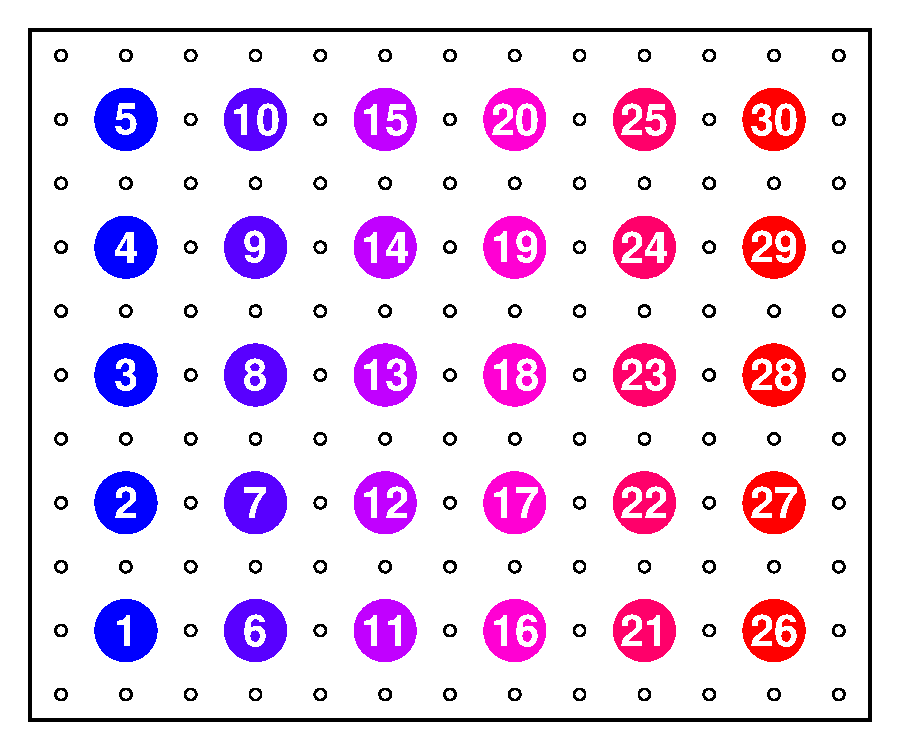
\includegraphics[width=1.8in,height=1.5in]{figs/sims/basic_lattice.pdf}}
		\subcaptionbox{barrier scenario \label{barrier_lattice}}
			{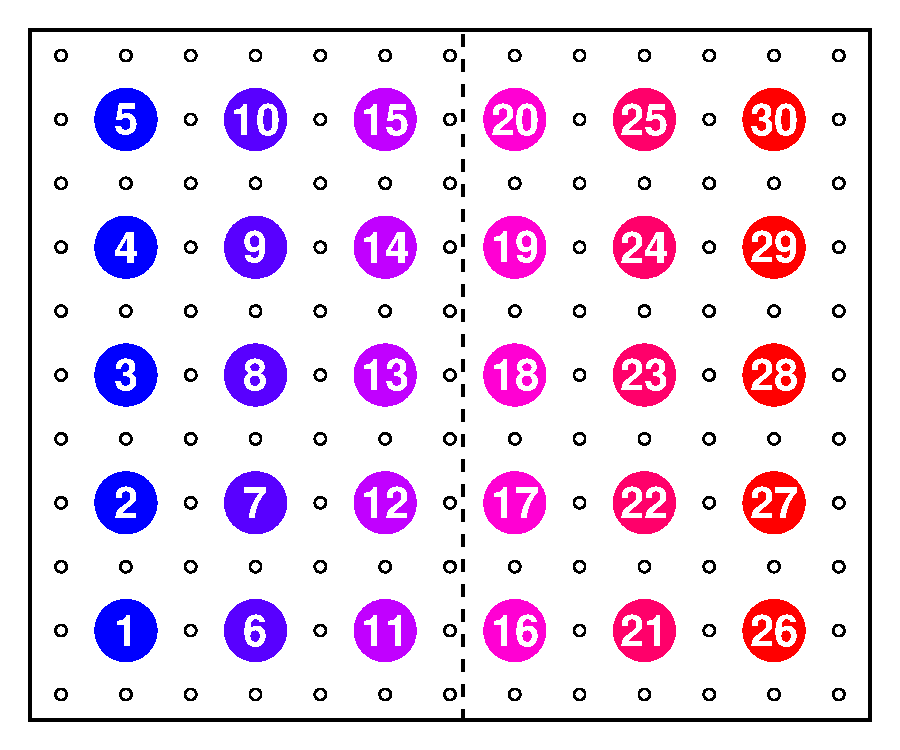
\includegraphics[width=1.8in,height=1.5in]{figs/sims/barrier_lattice.pdf}}
		\subcaptionbox{expansion scenario \label{expansion_lattice}}
			{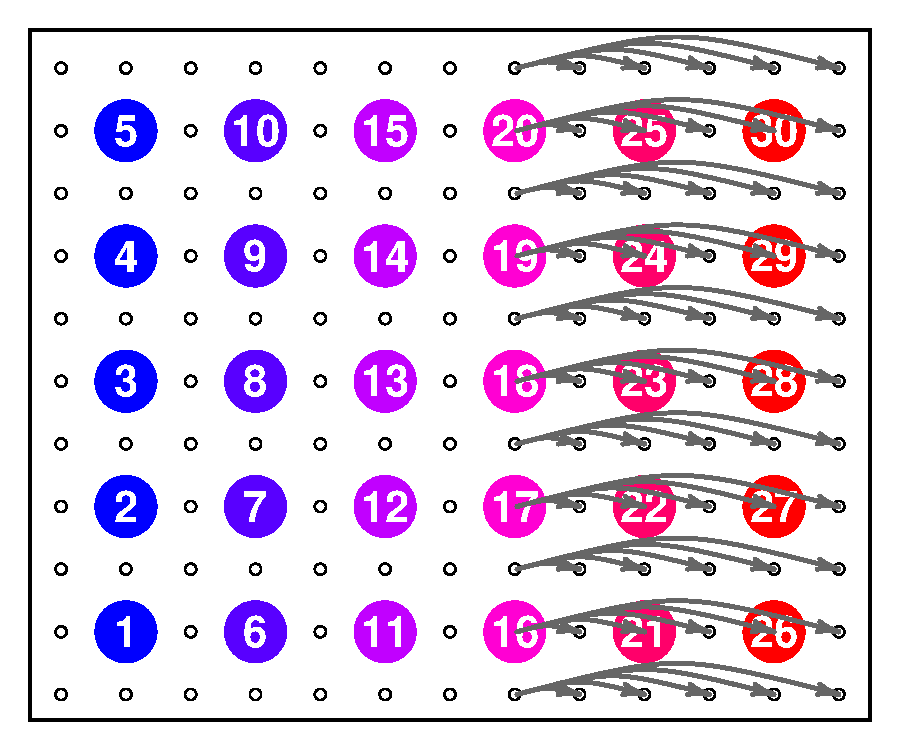
\includegraphics[width=1.8in,height=1.5in]{figs/sims/expansion_lattice.pdf}}
		\subcaptionbox{geogenetic map of \ref{sfig:lattice_scenarios}\subref{simple_lattice} \label{lattice_inference}}
			{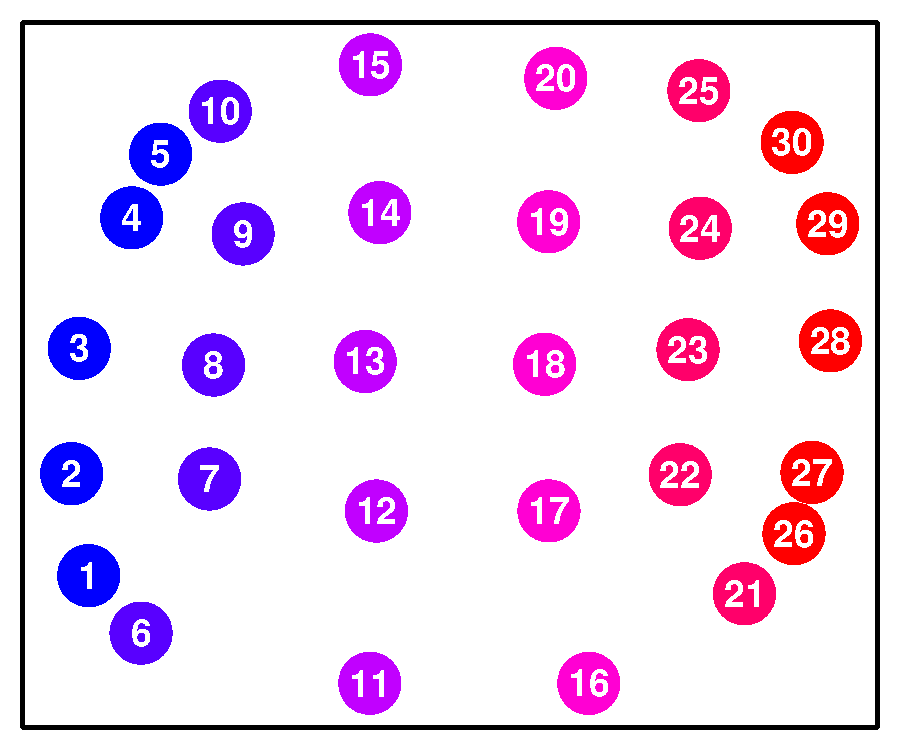
\includegraphics[width=1.8in,height=1.5in]{figs/sims/GeoGenMap_lattice.pdf}}
		\subcaptionbox{geogenetic map of \ref{sfig:lattice_scenarios}\subref{barrier_lattice}\label{barrier_inference}}
			{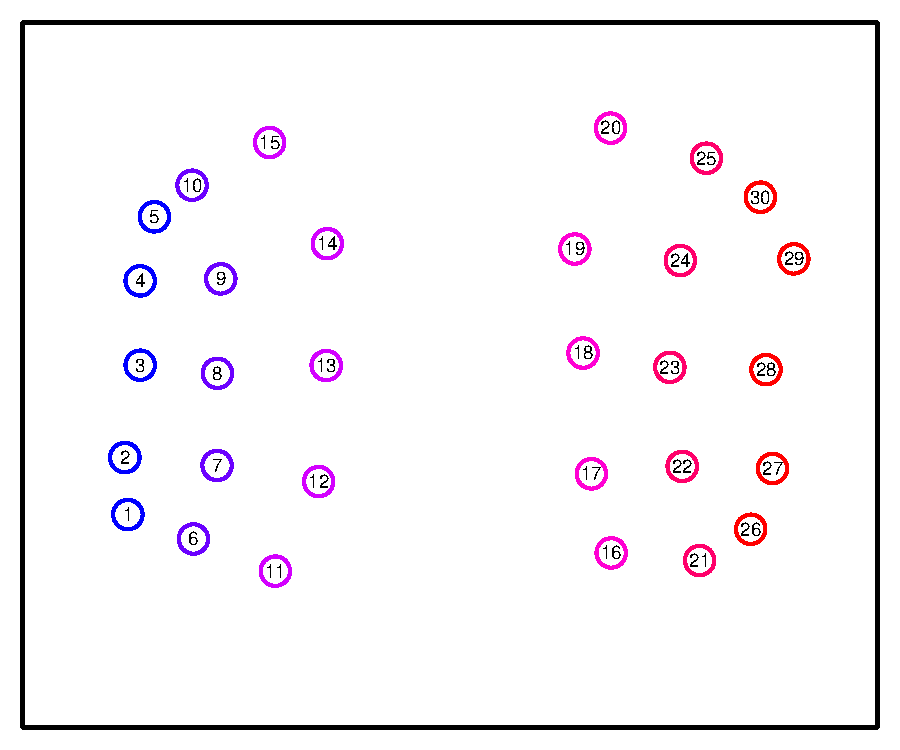
\includegraphics[width=1.8in,height=1.5in]{figs/sims/GeoGenMap_barrier.pdf}}
		\subcaptionbox{geogenetic map of \ref{sfig:lattice_scenarios}\subref{expansion_lattice} \label{expansion_inference}}
			{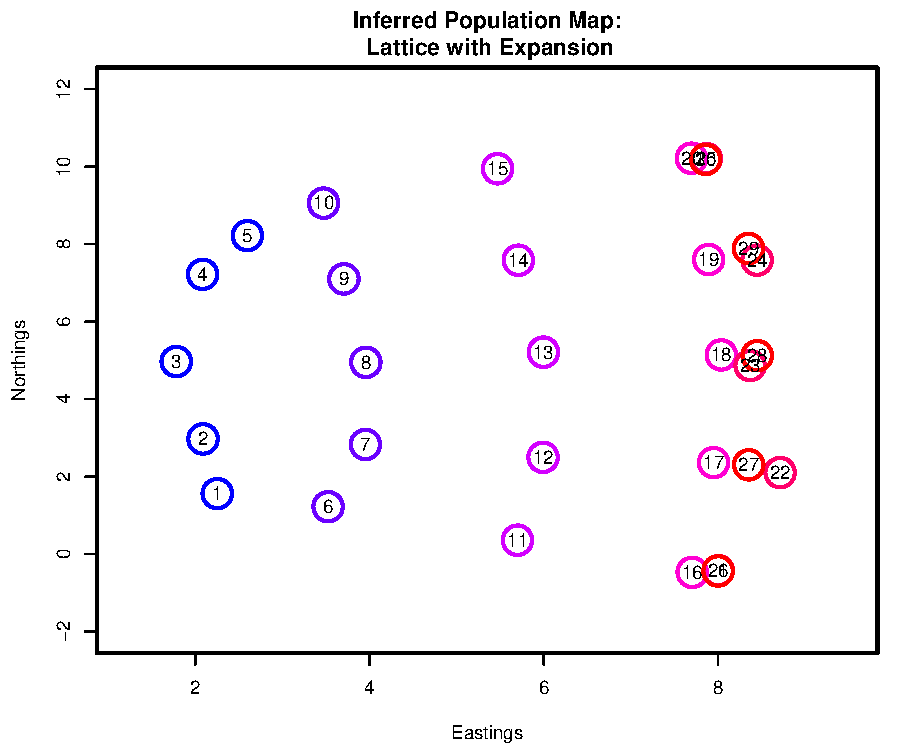
\includegraphics[width=1.8in,height=1.5in]{figs/sims/GeoGenMap_expansion.pdf}}

	\caption{
    Simulation scenarios and and their corresponding geogenetic maps estimated with SpaceMix.  
    The smaller, white dots in the simulation scenarios represent unsampled populations.  
    a) configuration of simulated populations on a simple lattice with spatially homogeneous migration rates; 
    b) a lattice with a barrier along the center line of longitude, across which migration rates are reduced by a factor of 5; 
    c) a lattice with recent expansion on the eastern margin; 
    d) the maximum \textit{a posteriori} (MAP) estimate from the posterior distribution of population locations under the scenario in \ref{sfig:lattice_scenarios}\subref{simple_lattice}, the simple lattice with homogeneous migration;  
    e) MAP estimate of population locations under the scenario in \ref{sfig:lattice_scenarios}\subref{barrier_lattice}, the lattice with a barrier; 
    f) MAP estimate of population locations under the scenario in \ref{sfig:lattice_scenarios}\subref{expansion_lattice}, the lattice with an expansion event.
    }\label{sfig:lattice_scenarios}
\end{figure}

The lattice scenarios, illustrated in Figure \ref{sfig:lattice_scenarios}, are: homogeneous migration rates across the grid; a longitudinal barrier across the center of the grid; a series of recent expansion events; and an admixture event between opposite corners of the lattice.  In the simple lattice scenario with homogeneous migration rates (Figs. \ref{sfig:lattice_scenarios}\subref{simple_lattice} and \ref{sfig:lattice_scenarios}\subref{lattice_inference}), SpaceMix recovers the lattice structure used to simulate the data (i.e., populations are correctly choosing their nearest neighbors).  
After adding a longitudinal barrier to dispersal across which migration rates are reduced by a factor of 5 (Fig.\ \ref{sfig:lattice_scenarios}\subref{barrier_lattice}), 
the two halves of the map are pushed farther away from one another, 
reflecting the increased effective distance between them.

In the expansion scenario, in which all populations in the last five columns of the grid have expanded simultaneously in the immediate past from the nearest population in their row (Fig.\ \ref{sfig:lattice_scenarios}\subref{expansion_lattice}), 
the daughter populations of the expansion event cluster with their parent populations, reflecting the higher relatedness (per unit of geographic separation) between them.  
In all scenarios, populations at the corners of the lattice are pulled in somewhat
because these have the least amount of data informing their relative placements.
In SuppMat Figs \ref{sfig:sim_covariance_decays}, we show the relationship between genetic covariance, geographic distance, and inferred geogenetic distance for these simulations.

We next simulated a long-distance admixture event on the same grid,
by sampling half of the alleles of each individual in the northeast corner population from the southwest corner population (Fig.\ \ref{sfig:corner_admix_scenarios}\subref{corner_admixture_lattice}).  We then ran a SpaceMix analysis in which the locations of these populations were estimated (Fig.\ \ref{sfig:corner_admix_scenarios}\subref{corner_admix_inference_CYOL}).
The admixture creates excess covariance over anomalously long distances, which is clearly difficult to accommodate with a two-dimensional geogenetic map.
Figure \ref{sfig:corner_admix_scenarios}\subref{corner_admix_inference_CYOL} shows the torturous lengths to which the method goes to fit a good geogenetic map: the admixed population 30 is between population 1, the source of its admixture, and populations 24, 25, and 29, the nearest neighbors to the location of its non-admixed portion.
However, this warping of space is difficult to interpret, and would be even more so in empirical data for which a researcher does not know the true demographic history.  

\begin{figure}
	\centering
		\subcaptionbox{simulated lattice with admixture \label{corner_admixture_lattice}}
			{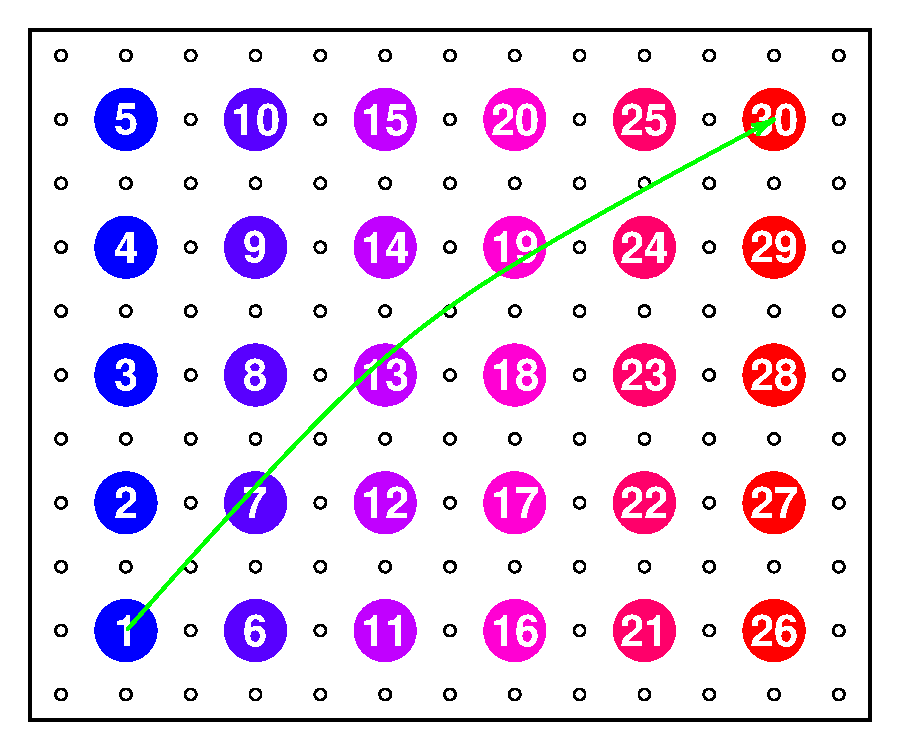
\includegraphics[width=2.8in,height=2.33in]{figs/sims/corner_admixture_lattice.pdf}}
		\subcaptionbox{geogenetic map without admixture inference \label{corner_admix_inference_CYOL}}
			{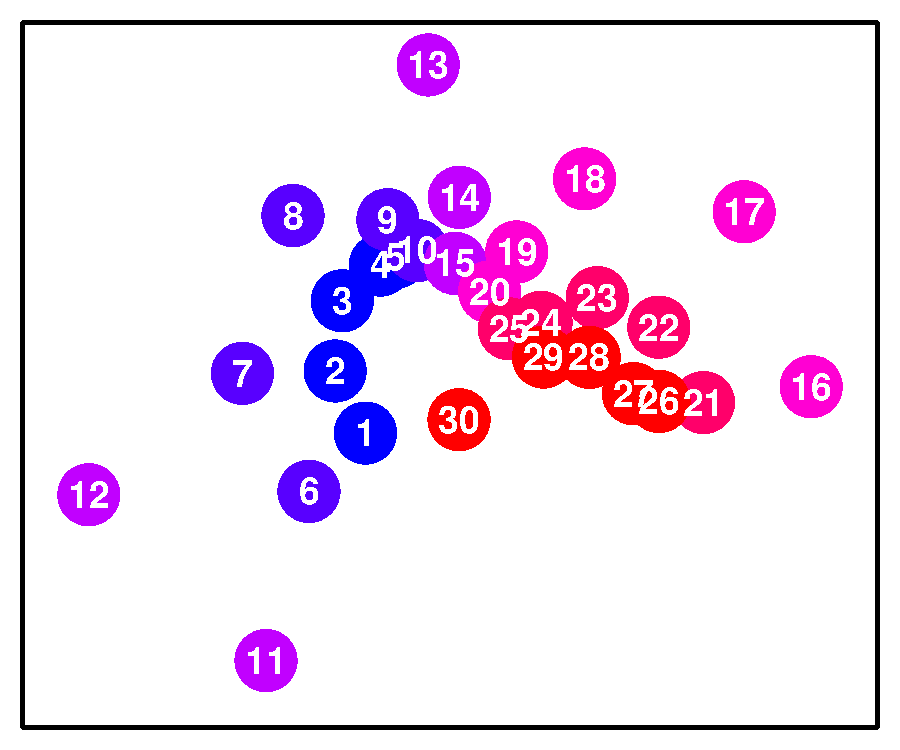
\includegraphics[width=2.8in,height=2.33in]{figs/sims/GeoGenMap_corner_admixture_CYOL.pdf}}
		\subcaptionbox{geogenetic map with admixture inference \gb{add legend} \label{corner_admix_inference}}
			{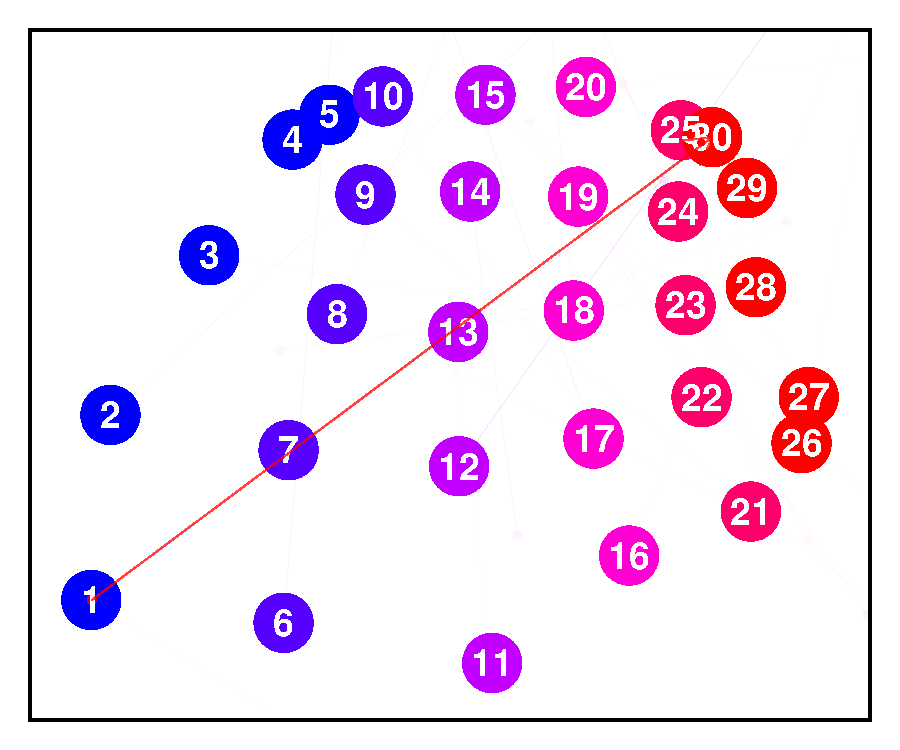
\includegraphics[width=2.8in,height=2.33in]{figs/sims/GeoGenMap_corner_admixture.pdf}}
	\caption{Simulation scenarios and SpaceMix inference.  a) a lattice with recent admixture event between population 1 in the southwest corner and population 30 in the northeast corner, so that population 30 is drawing half of its ancestry from population 1; b) the MAP estimate of population locations under this scenario; c) the MAP estimate of population locations and their sources of admixture under this scenario.  The 95\% credible interval on $w_{30}$ is 0.36 - 0.40. In panel (c), the width and opacity of the admixture arrows are drawn proportional the admixture proportions.}\label{sfig:corner_admix_scenarios}
\end{figure}



%%%%%%%%% %%%%%%%%% 
\subsection*{Inference of Spatial Admixture}

To incorporate recent admixture, we allow
each allele sampled in population $k$ to have a probability $w$ ($0 \leq w_k \leq 0.5$ ) of being sampled from location $\identifyadmixsource{G}_k$,
which we refer to as population $k$'s source of admixture,
and a probability $1-w$ of being sampled from location $G_k$.
With no nugget, each allele is sampled independently, but the nugget introduces correlations between the alleles sampled in each individual.
The population allele frequencies in population $k$ ($f^{\text{(pop)}}_k$) 
are then modeled as a weighted average of the allele frequencies at the geographic location the sampled population chooses for itself ($f_{k}$) 
and those at the coordinates of the source ($f_{\identifyadmixsource{k}}$) from which the observed population draws admixture.
\begin{equation}
f^{\text{(pop)}}_k = w_k f_{\identifyadmixsource{k}} + (1-w_k)f_{k}   \label{eqn-admixedfreq}
\end{equation}
We allow each of our populations an independent spatial source of admixture, as well as independent admixture proportions.

We can then consider the parametric covariance matrix of the standardized allele frequencies that follows from the form of the population frequencies in equation \eqref{eqn-admixedfreq}.  The admixed covariance between samples $i$ and $j$, $\identifyadmixsource{\Omega_{i,j}}$, is a function of all the pairwise spatial covariances between the locations of populations $i$ and $j$ and the points from which they draw admixture (illustrated in Figure \ref{sfig:admixed_cov_diagram}); by Equation \eqref{eqn-admixedfreq}, this form is as follows
\begin{alignat}{3}
\label{eq:admixed_covariance_1}
\identifyadmixsource{\Omega_{i,j}} = (1-w_i)(1-w_j) F(D_{i\;,\;j\;}) \; +&\\
w_i(1-w_j) F(D_{\identifyadmixsource{i},\;j\;}) \; +   \notag&\\
w_j(1-w_i) F(D_{i\;,\;\identifyadmixsource{j}}) \; +   \notag&\\
w_i w_j F(D_{\identifyadmixsource{i},\;\identifyadmixsource{j}}) \; +   \notag&\\
\delta_{i,j} (\eta_i + \frac{1}{\bar{S}_i}) \notag&
\end{alignat}

where $D$, dimension $2k \; \times \; 2k$, is a matrix of pairwise distances between all inferred locations and all sources of admixture (indexed by *), and for readability, we denote, e.g., $F(D(G_i,\identifyadmixsource{G}_j))$, as $F(D_{i\;,\;\identifyadmixsource{j}})$.
The spatial covariance, $F(D)$, is as given in Eqn.\ \eqref{eq:spatial_covariance}, and we reintroduce the nugget, $\eta_k$, and the sample size effect, $1/\bar{S_k}$, for each population as above in Eqn. \eqref{eq:spatial_covariance2}.

We proceed in our inference procedure as before, but now with the locations of the sources of admixture and the admixture proportions to infer.
The likelihood of our sample covariance matrix is Wishart:
\begin{equation}
\label{eq:wishart_dist_admixed}
P(\widehat{\Omega} \mid \identifyadmixsource{\Omega}) = 
	\mathcal{W}\left(L \widehat{\Omega} \mid \identifyadmixsource{\Omega} \left( G,\identifyadmixsource{G}, w,\vec{\alpha},\eta \right),L \right)
\end{equation}

The posterior probability of these parameters can be expressed as a function of this parametric admixed covariance, $\identifyadmixsource{\Omega}$,
\begin{equation}
\label{eq:admixed_post_prob}
P(G,\identifyadmixsource{G}, w,\vec{\alpha}, \eta \mid \widehat{\Omega}, L) 
	\propto  
		P(\widehat{\Omega}  \mid \identifyadmixsource{\Omega}) P(\vec{\alpha}) P(G) P(\identifyadmixsource{G}) P(w) P(\eta) 
\end{equation}
%
as specified by the parameters $w$, $\identifyadmixsource{G}$, $\vec{\alpha}$, and $\eta$, and the inferred locations, $G$.  
We place a weak spatial prior on the sources of admixture, $\identifyadmixsource{G}$ around the centroid of the observed locations. The admixture proportions, $w$, are capped at 0.5, to ensure identifiability,
and are heavily weighted towards small values to be conservative with respect to admixture inference.  
These priors are detailed in Table \ref{tab:param_prior_tab}.

\begin{figure}[htp!]
	\centering
	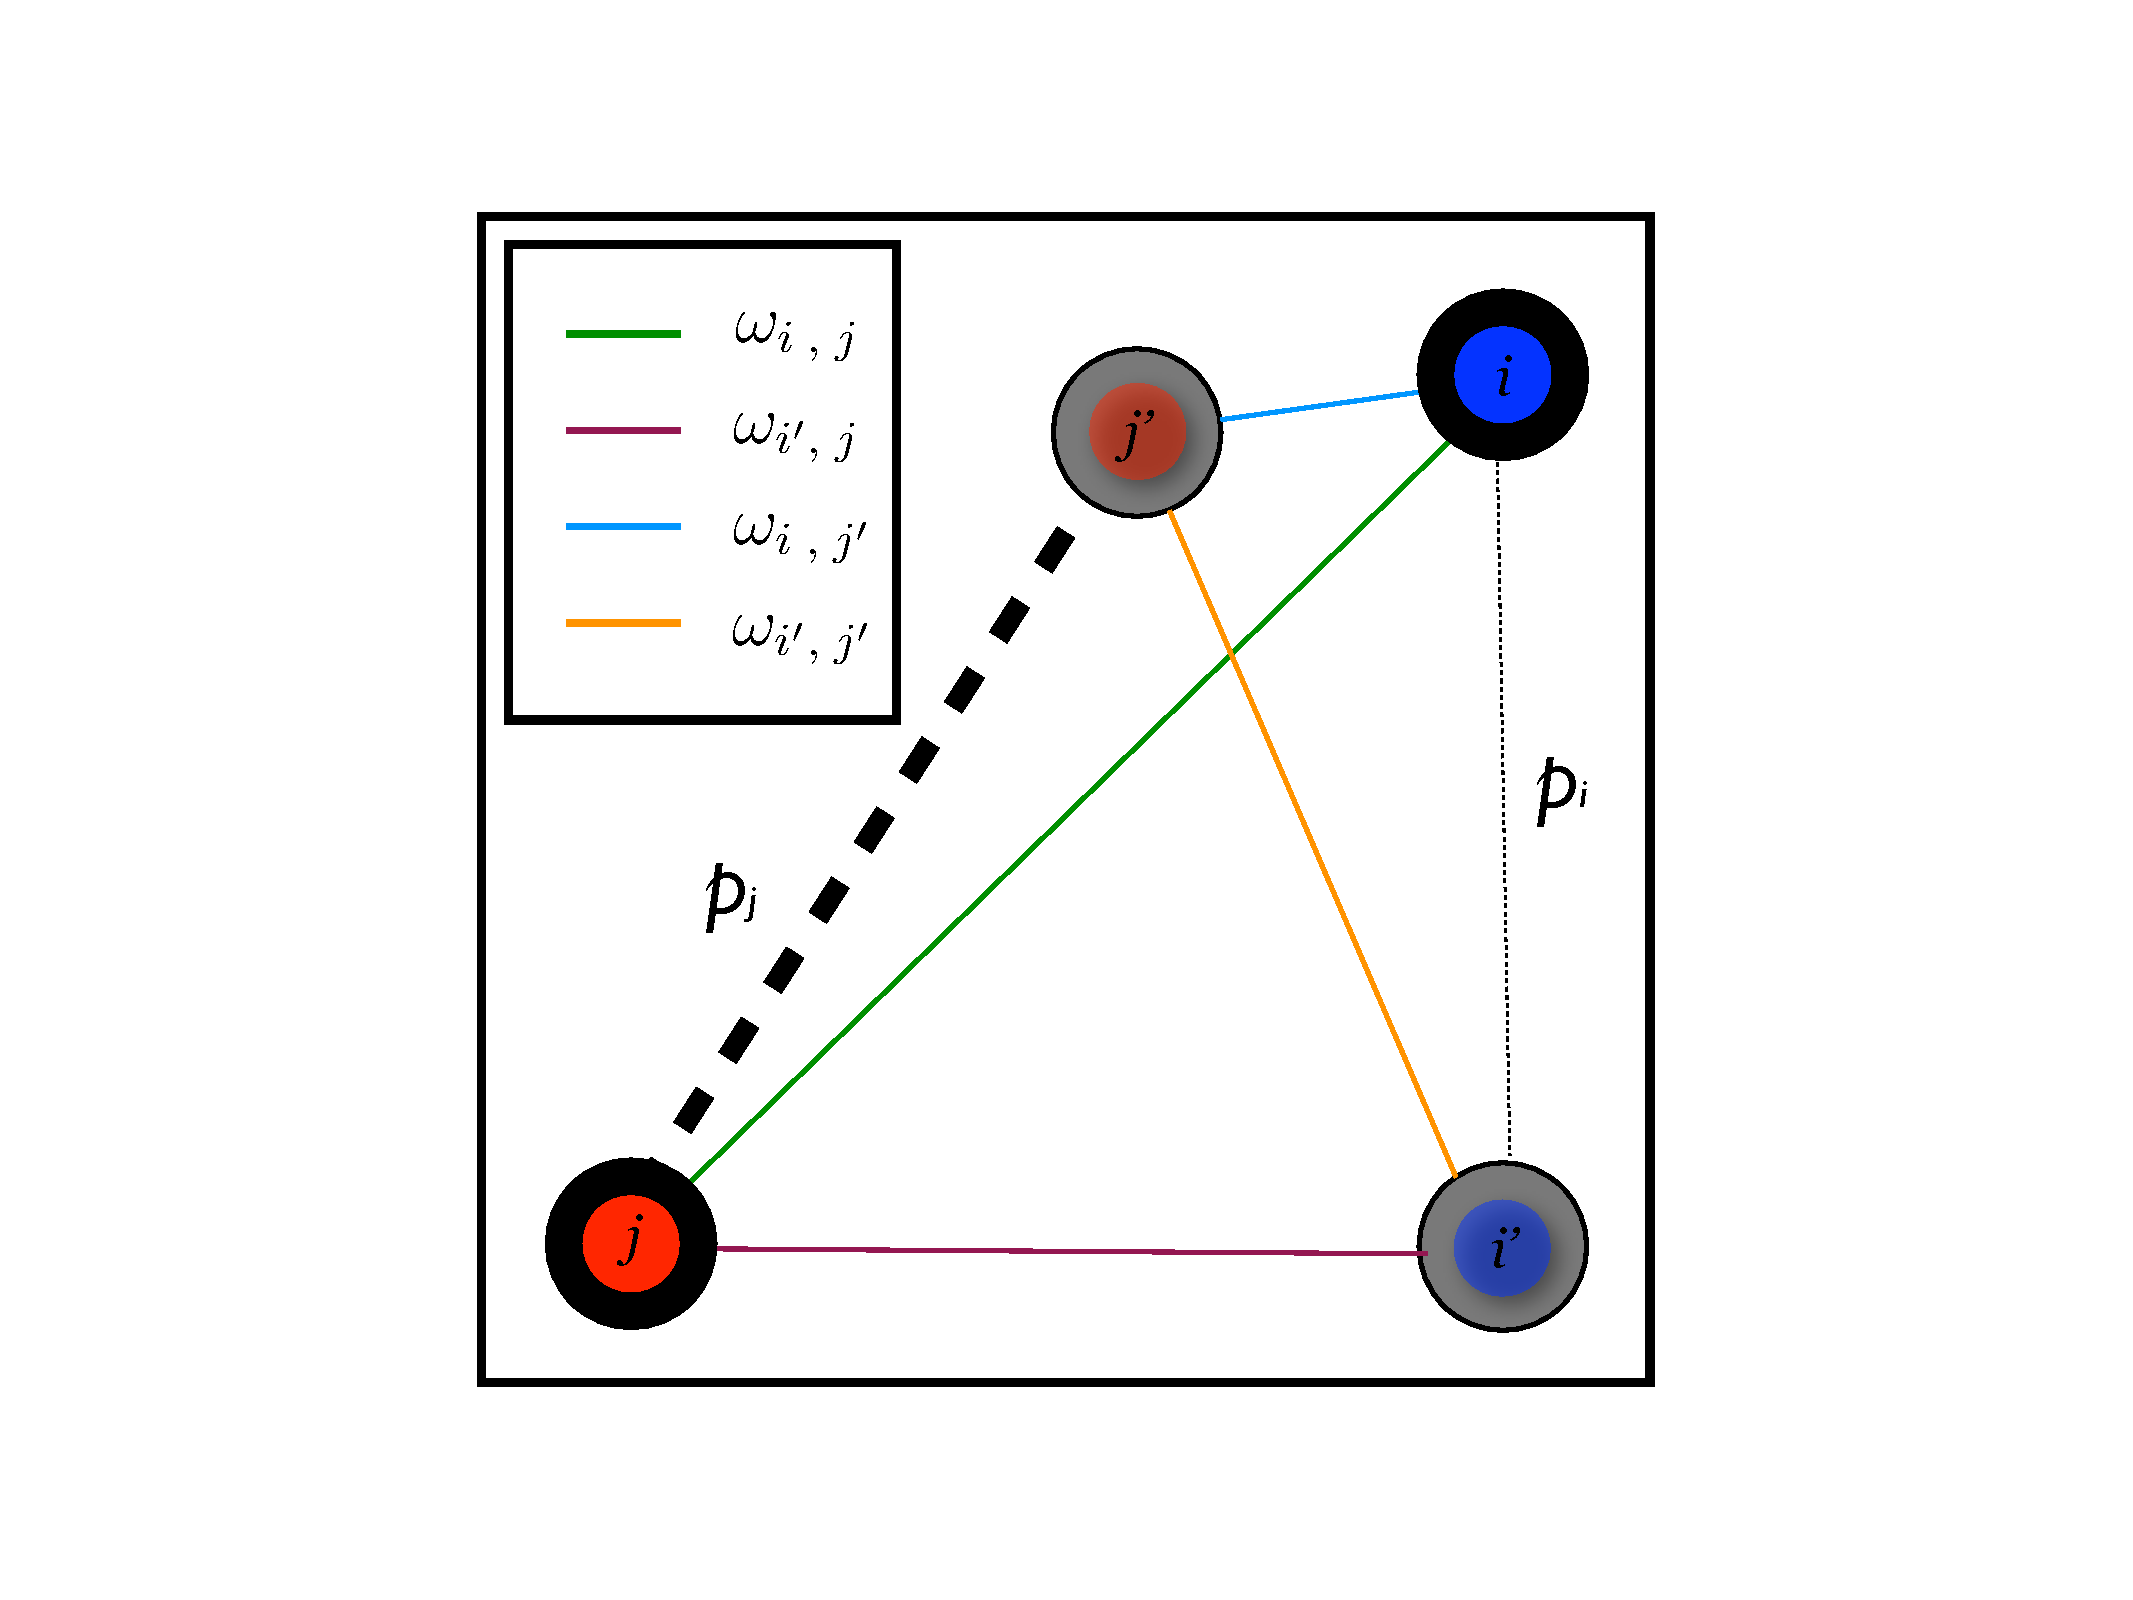
\includegraphics[width=2in,height=2in]{figs/admix_cov_fig.pdf}
	\caption{An illustration of the form of the admixed covariance given in Equation \eqref{eq:admixed_covariance_1}.  Populations $i$ and $j$ are drawing admixture in proportions $w_i$ and $w_j$ from their respective sources of admixture, $\identifyadmixsource{i}$ and $\identifyadmixsource{j}$, and all pairwise spatial covariances (the $F$'s) are shown.  In this cartoon example, population $j$ is drawing more admixture from its source $\identifyadmixsource{j}$ than $i$ is from its source $\identifyadmixsource{i}$ (i.e., $w_j > w_i$).
    }
\label{sfig:admixed_cov_diagram}
\end{figure}

%We treat the location of the source of admixture for population $k$, $\identifyadmixsource{G_k}$, and the population's admixture proportion, $p_k$, as random variables and jointly estimate them as part of our inference procedure. 

The models described above may be used in various combinations.  In the simplest model, populations do not choose their own locations, nor are they allowed to draw admixture; the only parameters to be estimated are those of the spatial covariance function given in equation \eqref{eq:spatial_covariance}, and the population-specific variance terms ($\eta_i$).  In the most complex model, population locations, the locations of their sources of admixture, and the proportions of admixture are all estimated jointly in addition to the parameters of the spatial covariance function and the population specific variances.  Users may wish to employ the more constrained models (e.g., fixing the locations or admixture proportions for some or all samples) in a model selection framework to test specific hypotheses.
% We discuss the identifiability of these models in the Methods.

Allowing admixture gives sensible results for the scenario of Figure \ref{sfig:corner_admix_scenarios}\subref{corner_admixture_lattice}:
in the resulting map,
the only population that draws substantial admixture is the one that is actually admixed, 
and it draws admixture (95\% CI: 0.36 - 0.40) from the correct location (Figure \ref{sfig:corner_admix_scenarios}\subref{corner_admix_inference}).

A more subtle simulated admixture scenario, with admixture proportion = 10\% across a geographic barrier, 
is shown Fig.\ \ref{sfig:barr_inland_ad}\subref{barr_inland_ad_scenario}).  
The resulting SpaceMix map (Fig.\ \ref{sfig:barr_inland_ad}\subref{barr_inland_ad_inference}), 
separates of the east and west sides of the grid to accommodate the effect of the barrier,
and the admixed population (population 23) chooses admixture from very close to its true source (population 13), 
and in close to the correct amount ($\bar{w}_{(23)} = 0.05; 95\% \text{CI} = 0.02-0.08$).

Another difficult scenario is shown in Figure \ref{sfig:barr_inland_ad}\subref{big_barr_ad_scenario},
where 40\% admixture has occurred between two populations immediately adjacent to each other on either side of a barrier.  
Here, the admixed population 23 is correctly identified as admixed, 
but it explains its intermediate genetic relationships by taking a location close to its true admixture source (population 13), 
and drawing admixture (95\% CI: 0.04 - 0.14) from a location on the far margin of the half of the grid on its own side of the barrier.
Because there is no sampled intervening population between admixed population 23 and its source of admixture 13, there is nothing to stop 23 from explaining its higher covariance with 13 via its chosen location $G_{(23)}$ rather than via that of its source of admixture $\identifyadmixsource{G}_{(23)}$.  
%However, 23 still has a lower variance than the other populations, and therefore must choose a proportion of admixture to accommodate that fact.  This analysis is a somewhat artificial example, as the biological interpretation of ``admixture" (defined in our spatial framework as anomalously long distance covariance) between near neighbors is unclear.
\gb{In each of these scenarios, the estimated admixture proportion is less than that used to simulate the data.  This is due to the stringent prior we place against admixture.  We discuss these examples further in the Appendix.}

\begin{figure}[htp!]
	\centering
		\subcaptionbox{`inland' admixture\label{barr_inland_ad_scenario}}
			{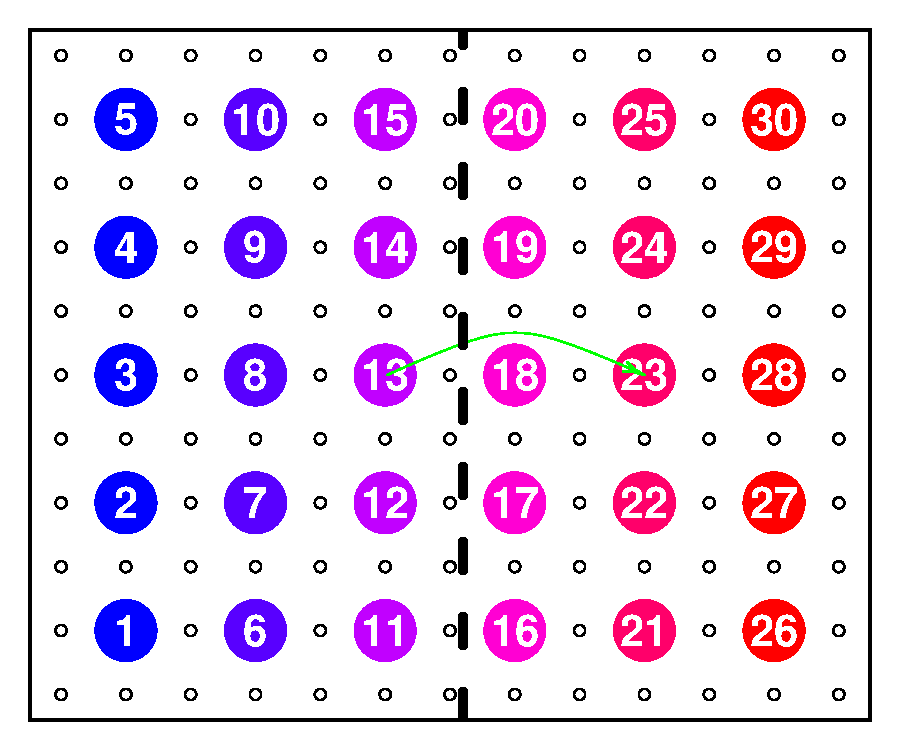
\includegraphics[width=2in,height=1.66in]{figs/sims/barr_inland_ad_lattice.pdf}}
		\subcaptionbox{`inland' geogenetic map \label{barr_inland_ad_inference}}
			{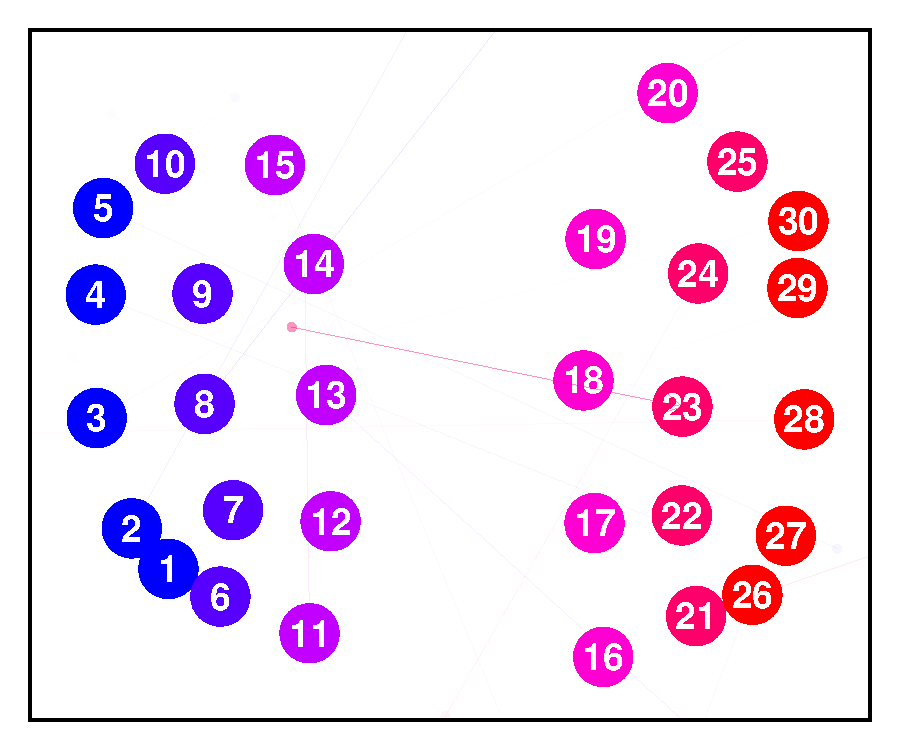
\includegraphics[width=2in,height=1.66in]{figs/sims/GeoGenMap_barr_inland_admixture_1.pdf}}
		\subcaptionbox{`neighbor' admixture \label{big_barr_ad_scenario}}
			{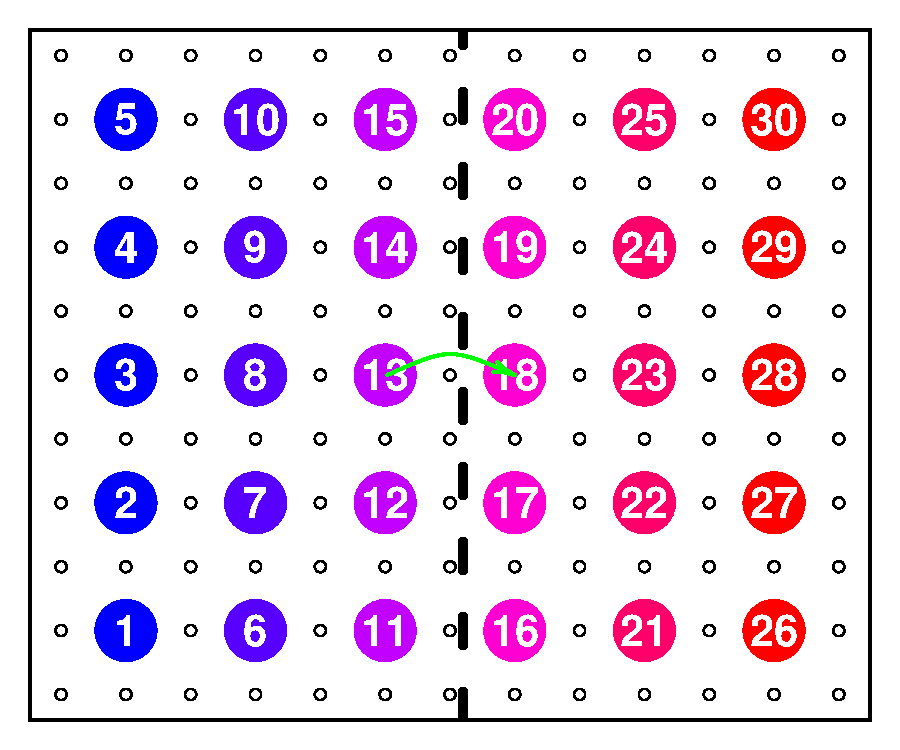
\includegraphics[width=2in,height=1.66in]{figs/sims/big_barr_ad_lattice.pdf}}
		\subcaptionbox{`neighbor' geogenetic map \label{big_barr_ad_inference}}
			{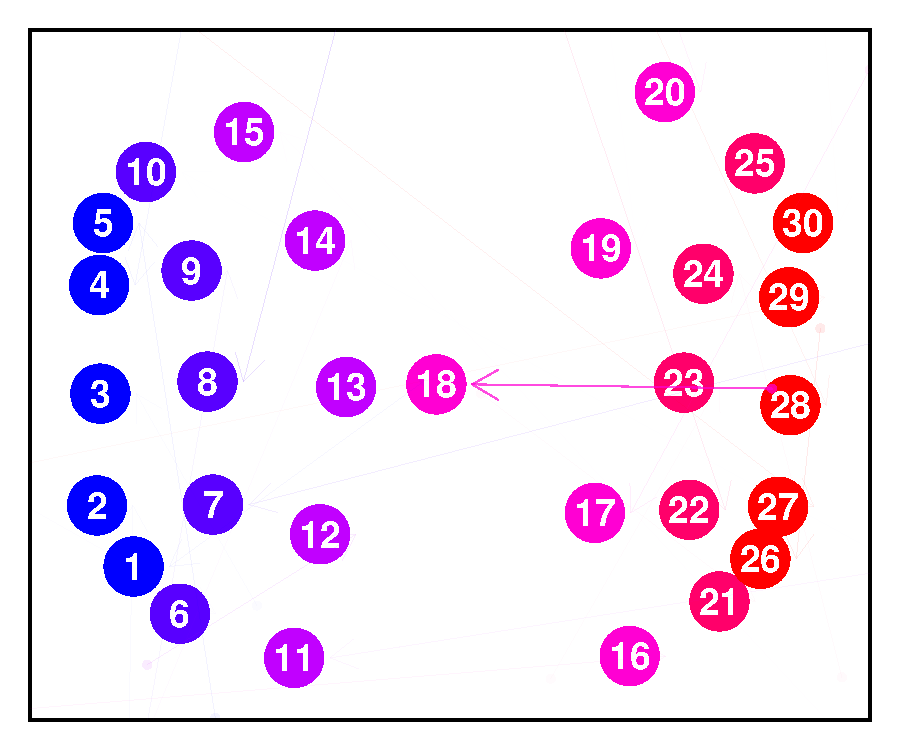
\includegraphics[width=2in,height=1.66in]{figs/sims/GeoGenMap_big_barr_ad_1.pdf}}
	\caption{
    Simulation scenarios and inferred population maps for two different admixture scenarios: a) lattice with a barrier and an admixture event (10\%) across the barrier to an `inland' population; b) the inferred population map for the scenario in (a), where the admixed population 23 is the only population drawing non-negligible admixture (95\% CI: 0.02-0.08) ; c) lattice with a barrier and an admixture event (40\%) across the barrier to a `neighbor' population on the border of the barrier; (d) the inferred population map for the scenario in (c), where the admixed population 18 is the only population drawing non-negligible admixture (95\% CI: 0.04 - 0.14).
}\label{sfig:barr_inland_ad}
\end{figure}


\section*{Empirical Applications}
To demonstrate the applications of this novel method, we analyzed population genomic data from two systems: the greenish warbler ring species complex, and a global sampling of contemporary human populations.  Maps showing our sampling in these two systems are shown in Figure \ref{sfig:empirical_maps}, and information on the specific populations included is given in the Supplementary Materials, Tables \ref{tab:warbler_data_table} and \ref{tab:globe_data_table}.  
For all analyses presented below, we used random `observed' locations as the priors on population locations.
For clarity and ease of interpretation, we then present a full Procrustes superimposition of the inferred population locations ($G$) and their sources of admixture ($\identifyadmixsource{G}$), using the observed latitude and longitude of the populations/individuals to give a reference position and orientation.

\begin{figure}
	\centering
		\subcaptionbox{Warbler subspecies distribution map \label{irwin_map}}
			{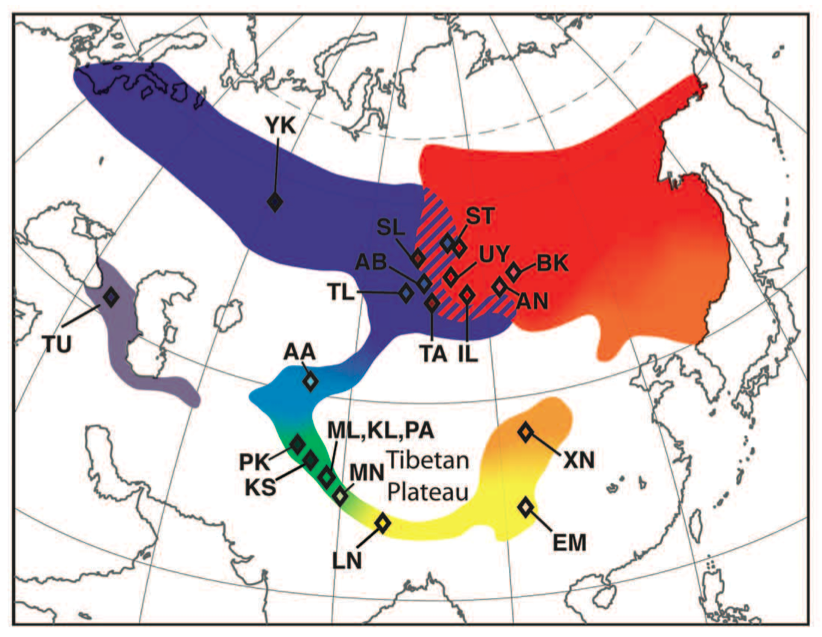
\includegraphics[width=2in,height=1.66in]{figs/warblers/Irwin_warbler_map_figure.png}}
		\subcaptionbox{Human sample distribution map \label{human_map}}
			{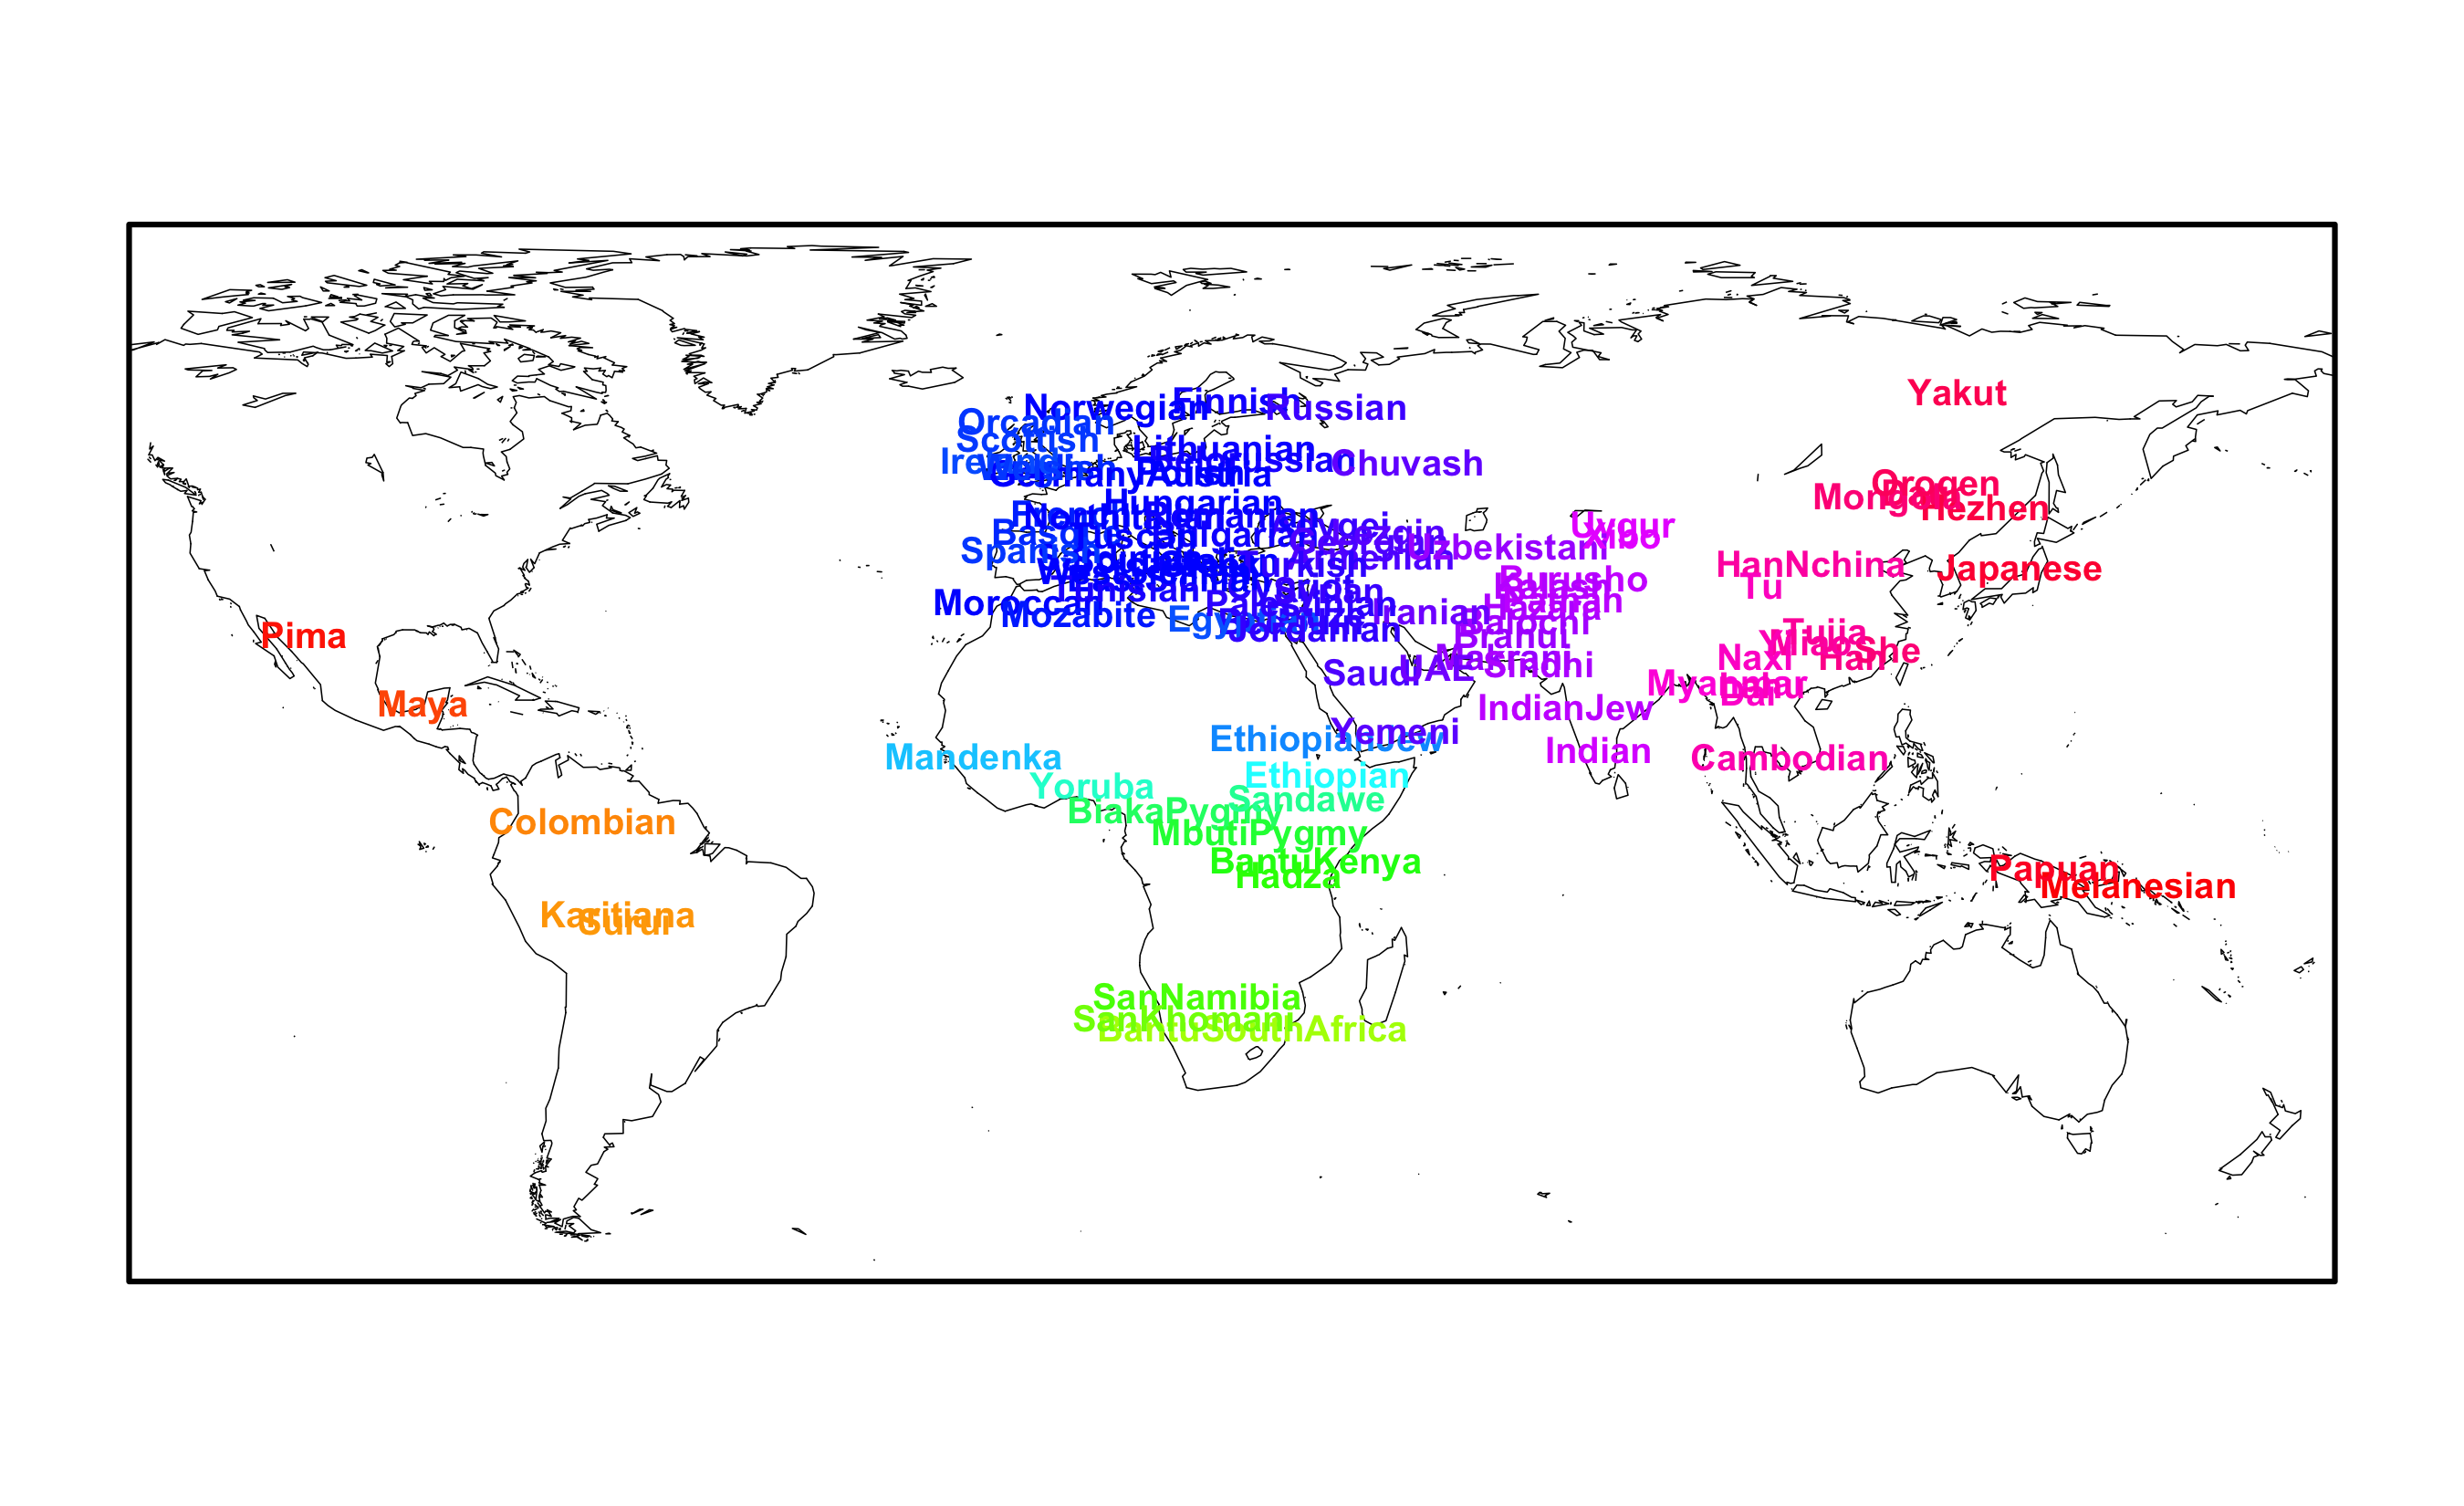
\includegraphics[width=4in,height=2.4in]{figs/globetrotter/globe_world_map_text.png}}
            \caption{Sampling maps of both empirical systems analyzed.  (a) greenish warbler subspecies distributions of all 22 sampled populations (breeding grounds), consisting of 95 individuals; (b) sampling map for human dataset, consisting of 1,490 individuals from 95 sampling locations.}
\label{sfig:empirical_maps}
\end{figure}


\subsection*{Greenish Warblers}  
%However, we note that many would still classify this as a ring species even if that condition were not met, just not as a case of speciation-by-distance (

The greenish warbler (\textit{Phylloscopus trochiloides}) species complex is broadly distributed around the Tibetan plateau, and exhibits gradients around the ring in a range of phenotypes including song, as well as in allele frequencies (Ticehurst (1938), Irwin et al 2001, Irwin et al 2005, Irwin et al 2008).  At the northern end of the ring in central Siberia, where the eastern and western arms of population expansion meet, there are discontinuities in call and morphology, as well as reproductive isolation and a genetic discontinuity (Irwin et al 2001, Irwin et al 2008). It is proposed that the species complex represents a ring species, in which selection and/or drift, acting in the populations as they spread northward on either side of the Tibetan plateau, have led to the evolution of reproductive isolation between the terminal forms (REFs).  

The question of whether it fits the most strict definition of a ring species focuses on whether gene flow along the margins of the plateau has truly been continuous throughout the history of the expansion or if, alternatively, discontinuities in migration around the species complex's range have facilitated periods of differentiation in genotype or phenotype without gene flow (Mayr 1942, Mayr 1970, Coyne and Orr 2004, see Wake and Schneider 1998 for discussion). 
\citet{alcaide2014genomic} have suggested that the greenish warbler species complex constitutes a `broken' ring species, in which historical discontinuities in gene flow have facilitated the evolution of reproductive isolation between adjacent forms.  

To investigate this question, we applied SpaceMix to the dataset from \citet{alcaide2014genomic}, 
consisting of 95 individuals sampled at 22 distinct locations and sequenced at 2,334 SNPs, of which 2,247 were bi-allelic and retained for SpaceMix runs.
The libraries were prepared using a genotype-by-sequencing protocol and were run on an Illumina HiSeq 2000 with a paired-end sequencing protocol.

\begin{figure}
	\centering
		\subcaptionbox{Warbler population map, no admixture \label{warb_pop_noad}}
			{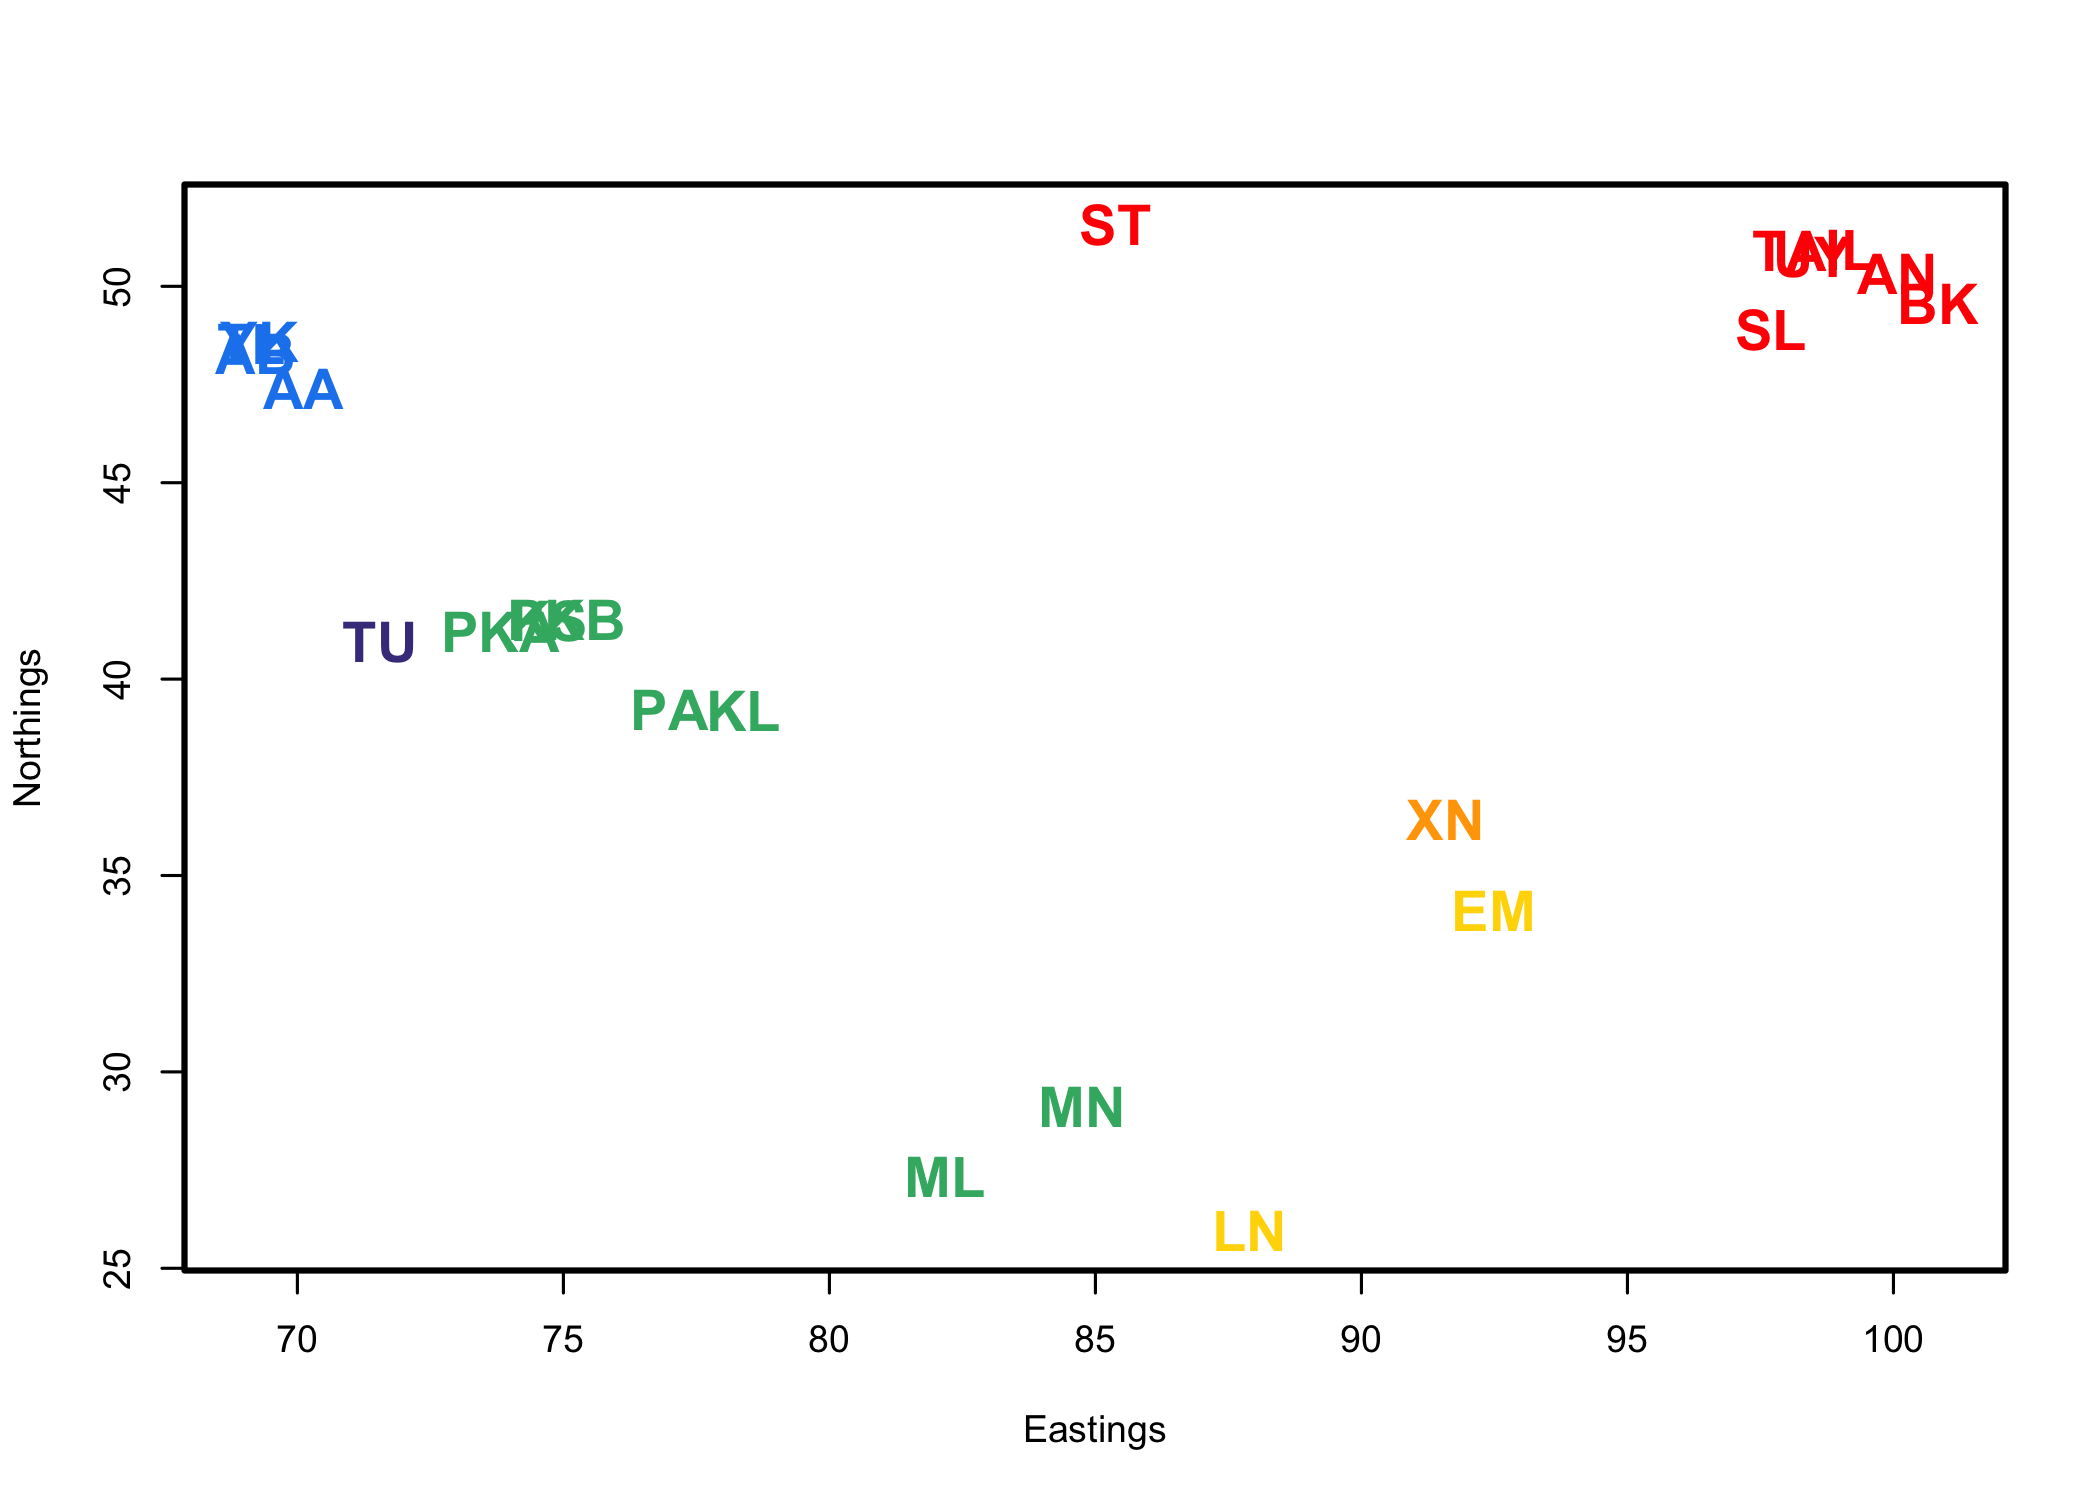
\includegraphics[width=2.4in,height=2in]{figs/warblers/warb_pop_noad.png}}
		\subcaptionbox{Warbler population map, with admixture \label{warb_pop_ad}}
			{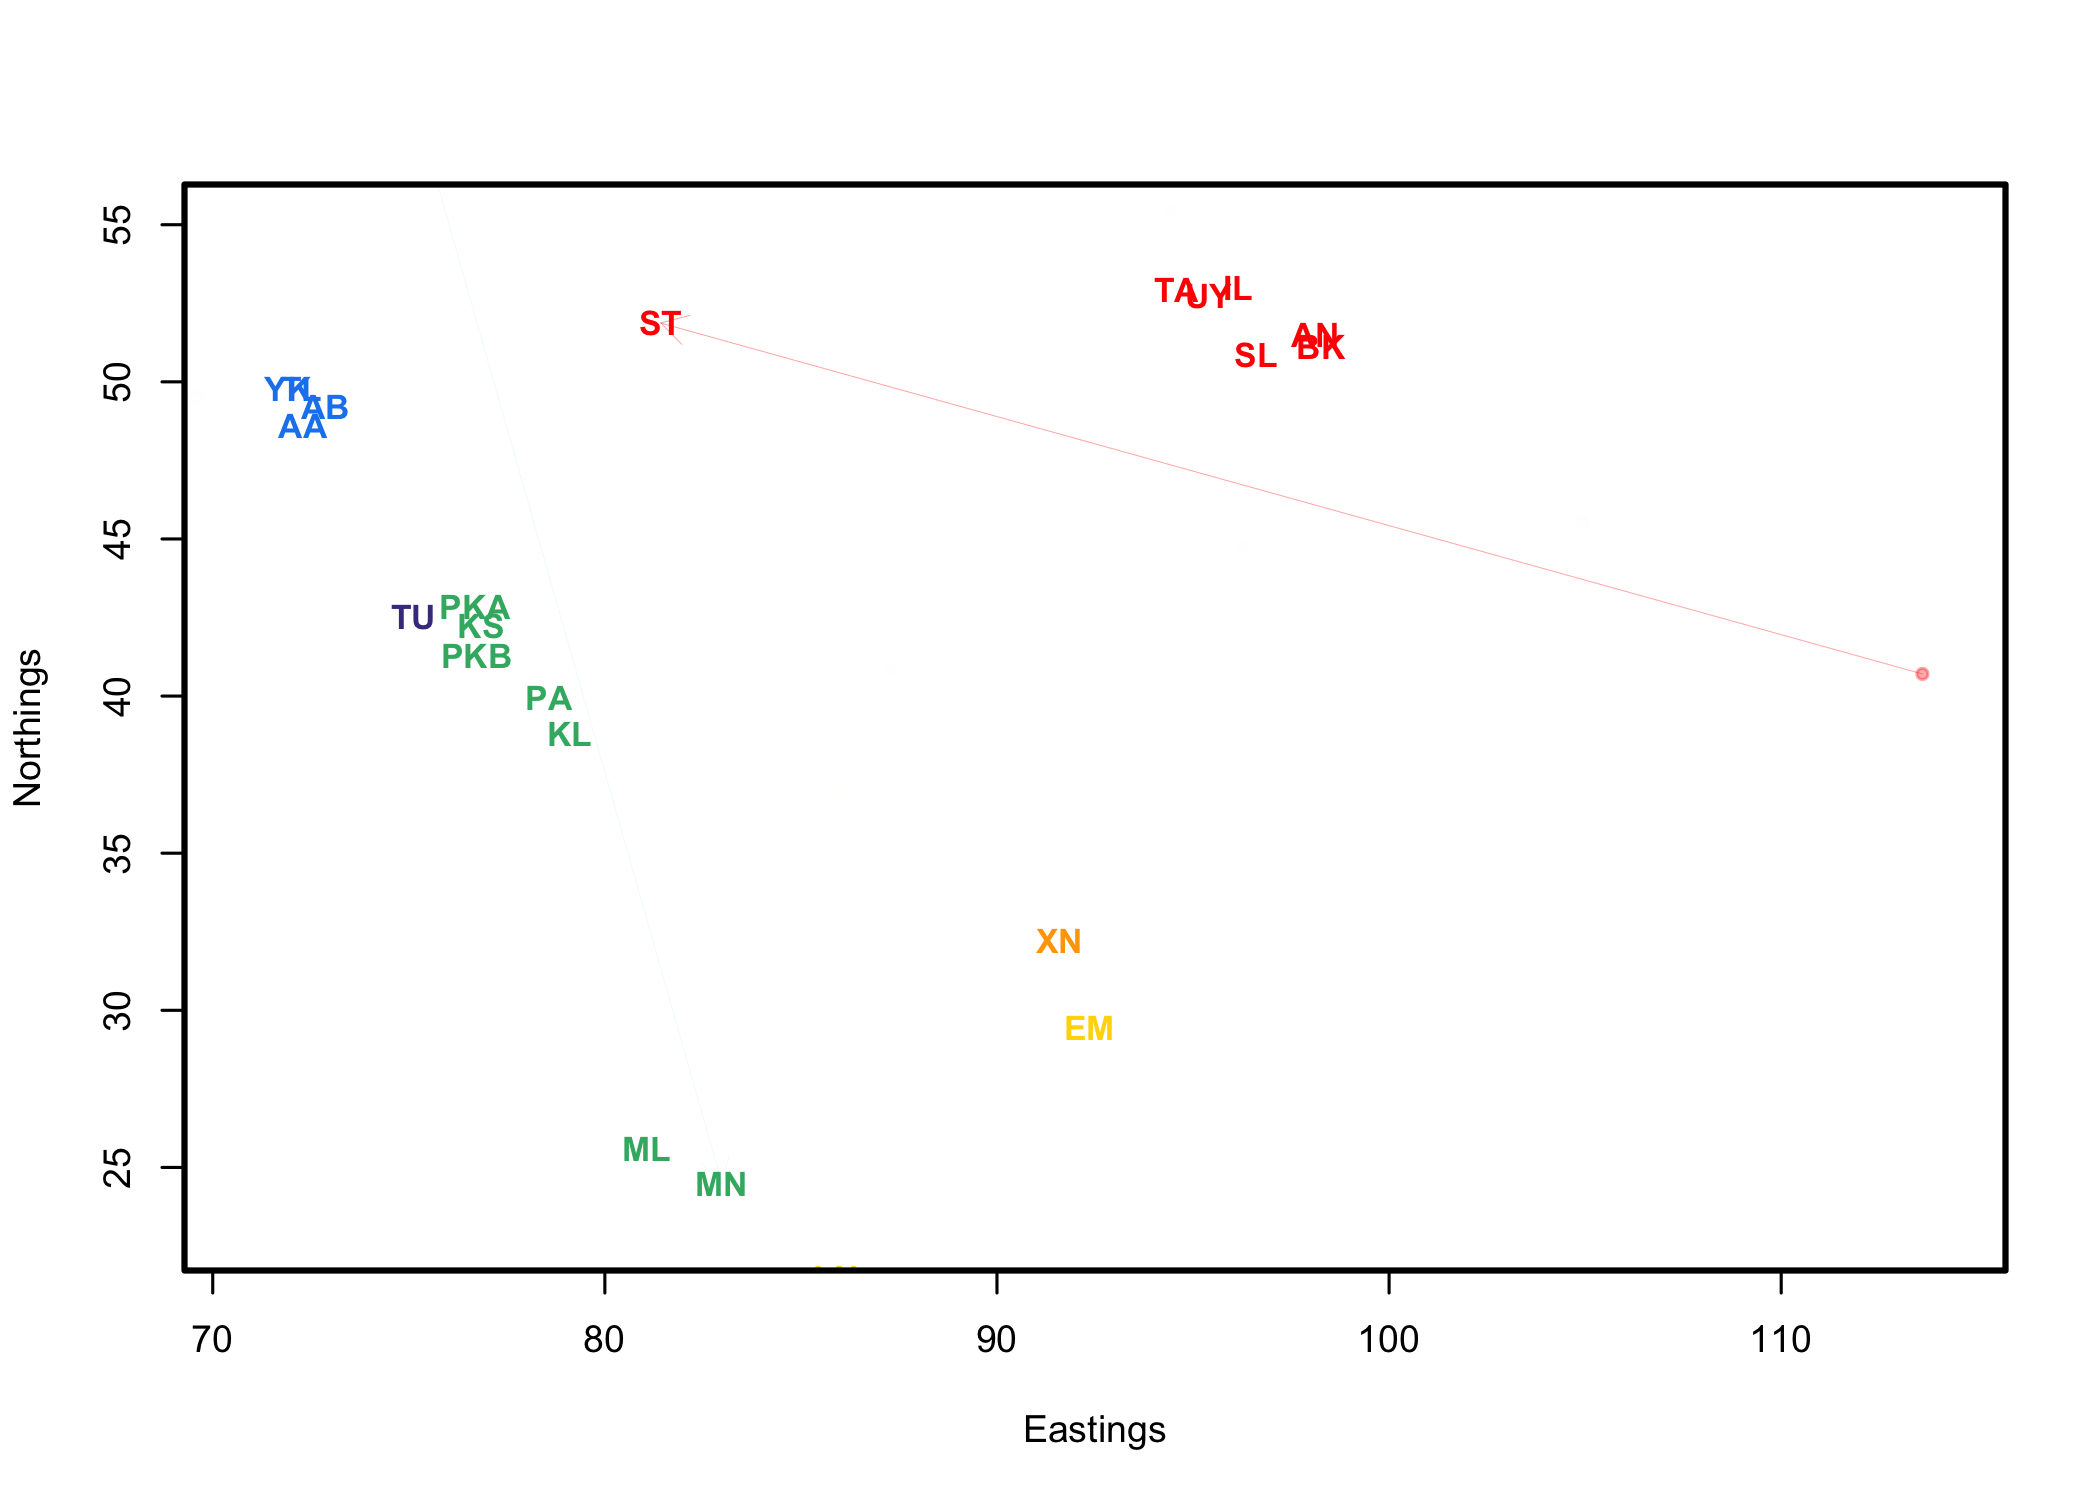
\includegraphics[width=2.4in,height=2in]{figs/warblers/population_warbler_map_randpr1.png}}
\caption{Inferred population maps with population labels colored as in Fig.\ \ref{sfig:empirical_maps}\subref{irwin_map}: a) the map inferred with no admixture inference; b) the map inferred with admixture inference.}
\label{sfig:warbler_pop}
\end{figure}

%\plr{
%I suggest a different order to the results.  Rather than populations, populations with admixture, individuals with admixture (confusing!)
%how about: Results are (individuals with admixture).
%Then, maybe in the appendix: for illustration, here's what would have happened without splitting out individuals.  
%Particularly because it's weird to call ST a ``population'' when we knew there's warblers from two different subspecies.
%I'm not clear if we need the "without admixture" at all?
%Maybe it is useful for comparing to PCA, which would put the admixed pop intermediate?
%}

%The Yekat population (\textbf{YK}) of \textit{viridanus} individuals clusters closely with the other, less far-flung \textit{viridanus} individuals, indicating that differentiation within that subspecies is incommensurate with the amount of IBD expected for samples separated by that much distance. 

We first ran SpaceMix on the population dataset, with no admixture. The resulting inferred map (Figure \ref{sfig:warbler_pop}\subref{warb_pop_noad}) largely recapitulates the geography of the sampled populations around the ring.  The Turkish population (\textbf{TU}, \textit{Phylloscopus trochiloides} ssp.\ \textit{nitidus}) clusters with the populations in the subspecies \textit{ludlowi}, due to its recent expansion, but also chooses a relatively high nugget parameter (see SuppMat Fig \ref{sfig:warb_pop_NoAd_nugg}), reflecting the population history it does not share with its \textit{ludlowi} neighbors.  In the North, where the twin waves of expansion around the Tibetan Plateau are hypothesized to meet, the inferred geogenetic distance between populations from either side of the ring was much greater than their observed geographic separation, reflecting the reproductive isolation between these adjacent forms (see Supplementary Figure \ref{sfig:warb_pop_distcomp}).  

%Interestingly, the six individuals sampled in Stolby, Russia, (\textbf{ST}) choose a location intermediate between the \textit{plumbeitarsus} and \textit{viridanus} groups. In the case where no admixture is allowed, this population is forced to adopt an intermediate position to fit its admixed nature.

%However, where the population-level analysis shows the Stolby population intermediate between the \textit{viridanus} and \textit{plumbeitarsus} clusters, the individual-level analysis reveals that the Stolby population (n=6) ,

% and again discuss the results from the analysis using random locations as priors on $G^{\prime}$

We then ran the method allowing admixture (Figure \ref{sfig:warbler_pop}\subref{warb_pop_ad}). The only population sample with appreciable admixture is the Stolby sample ($w=0.19$ (95\% credible interval: 0.146-0.238).  This sample is known to be composed of an equal mixture of eastern \textit{plumbeitarsus} and western \textit{viridanus} individuals \citep{alcaide2014genomic}. Multiple runs agreed well on the level of admixture of the Stolby sample (see Supplementary Figure \ref{sfig:warbler_pop_compare}). What does vary across runs is whether the Stolby sample chooses to locate itself by the \textit{viridanus} cluster and draw admixture from near the \textit{plumbeitarsus}  cluster or vise versa; however, this is to be expected given the 50/50 nature of the sample's makeup (Supplementary Figure \ref{sfig:warbler_pop_compare}). The somewhat intermediate position of the Stolby sample, and its non-50/50 admixture proportion, likely partially reflect the influence of the priors (Supplementary Figure \ref{sfig:warbler_pop_compare}). 

%In these analyses, the sample size in each `population' was 2 (for the two haplotypes in a diploid), and each individual chose its own location as well as the location of its source of admixture, the proportion of that admixture, and its nugget.  

%Because \textit{a priori} assigned population membership may be artificial (individuals from more than one population may be sampled at a single site), 
%\plr{and also, why not? it is clearly better, if possible?}
We repeated these analyses (with and without admixture) on an individual level (Figure \ref{sfig:warbler_ind_maps}).  
No individual drew appreciable admixture (see SuppMat Fig \ref{sfig:warb_ind_adprops} for admixture proportions), and so we discuss the results with admixture (those without admixture are nearly identical, see SuppMat Figure \ref{sfig:warbler_ind_maps_compare}).  As with the analysis on multi-sample populations, the results approximately mirror the geography of the individuals.

% (individuals in the admixture analysis choose very low levels of admixture (see SuppMat Figure \ref{sfig:warb_ind_adprops}); the population with the highest admixture proportion draws has a mean of 0.012 ($1.46 \times 10^{-4}$ to $4.73 \times 10^{-2}$)), 
%we discuss only the analysis with admixture inference

%The order of individuals' estimated locations around the Plateau is largely concordant with their true locations, and, in most cases, individuals sampled from the same population cluster closely together, as would be expected if samples collected at a single site are draws from a population that is locally panmictic.  
%\gb{could drop panels (A) and (B)}
\begin{figure}
	\centering
		\subcaptionbox{Warbler individuals map, admixture \label{warb_ind_ad}}
			{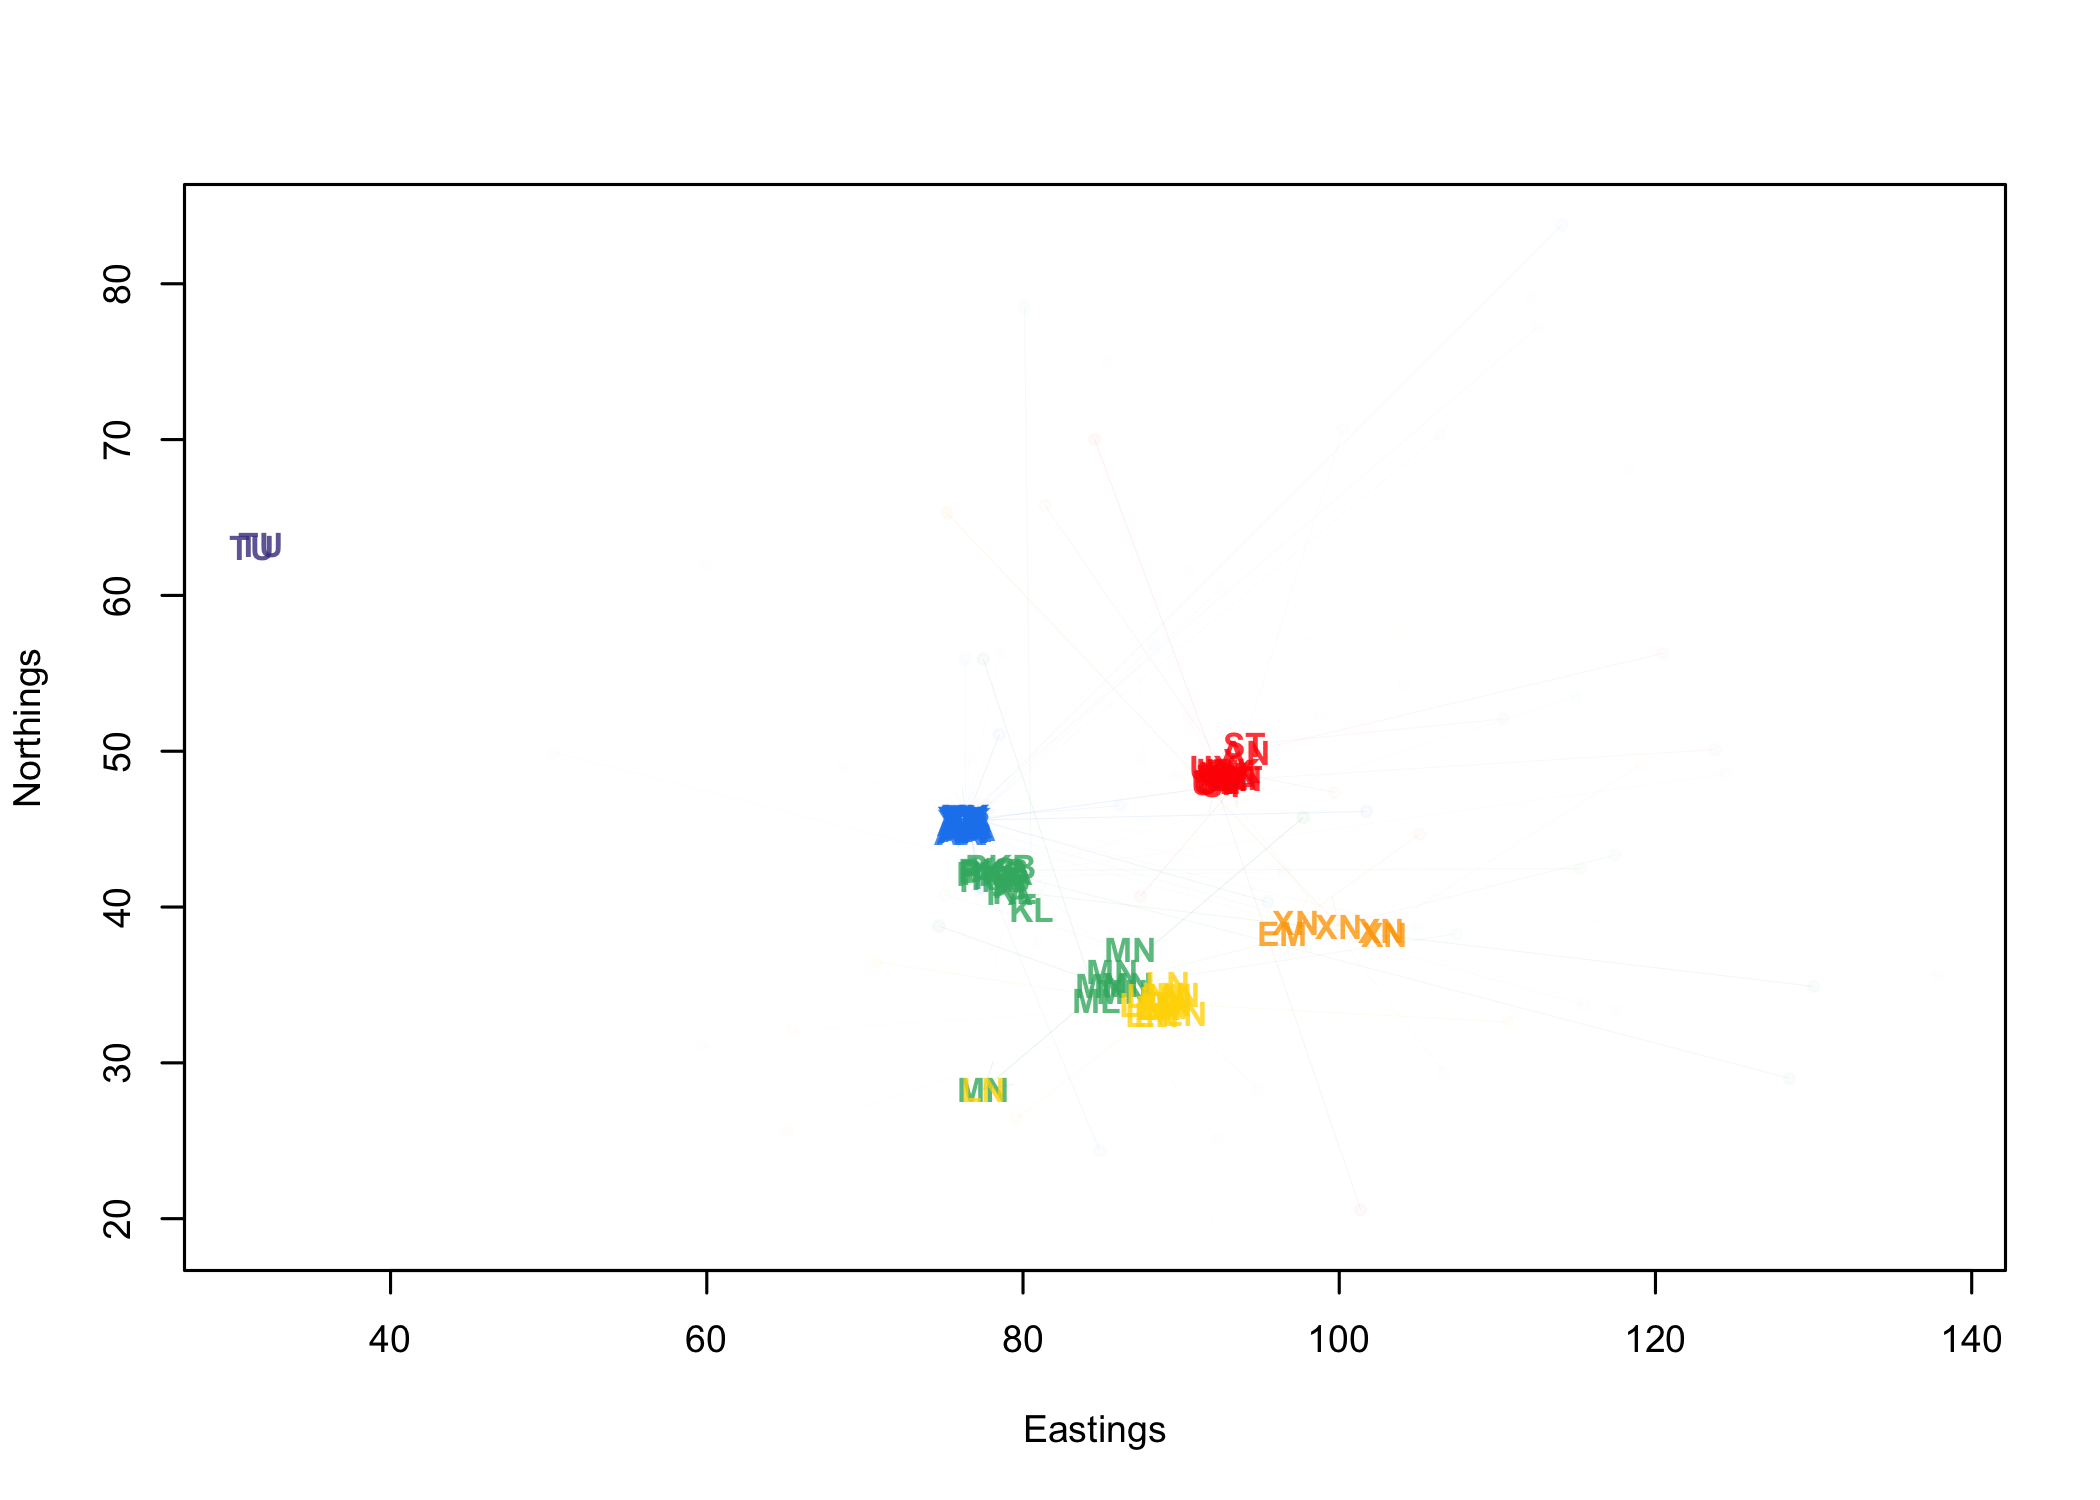
\includegraphics[width=2.8in,height=2.3in]{figs/warblers/individual_warbler_map_arrows_randpr1.png}}
		\subcaptionbox{Closeup of non-\textit{nitidus} samples \label{warb_ind_ad_closeup}}
			{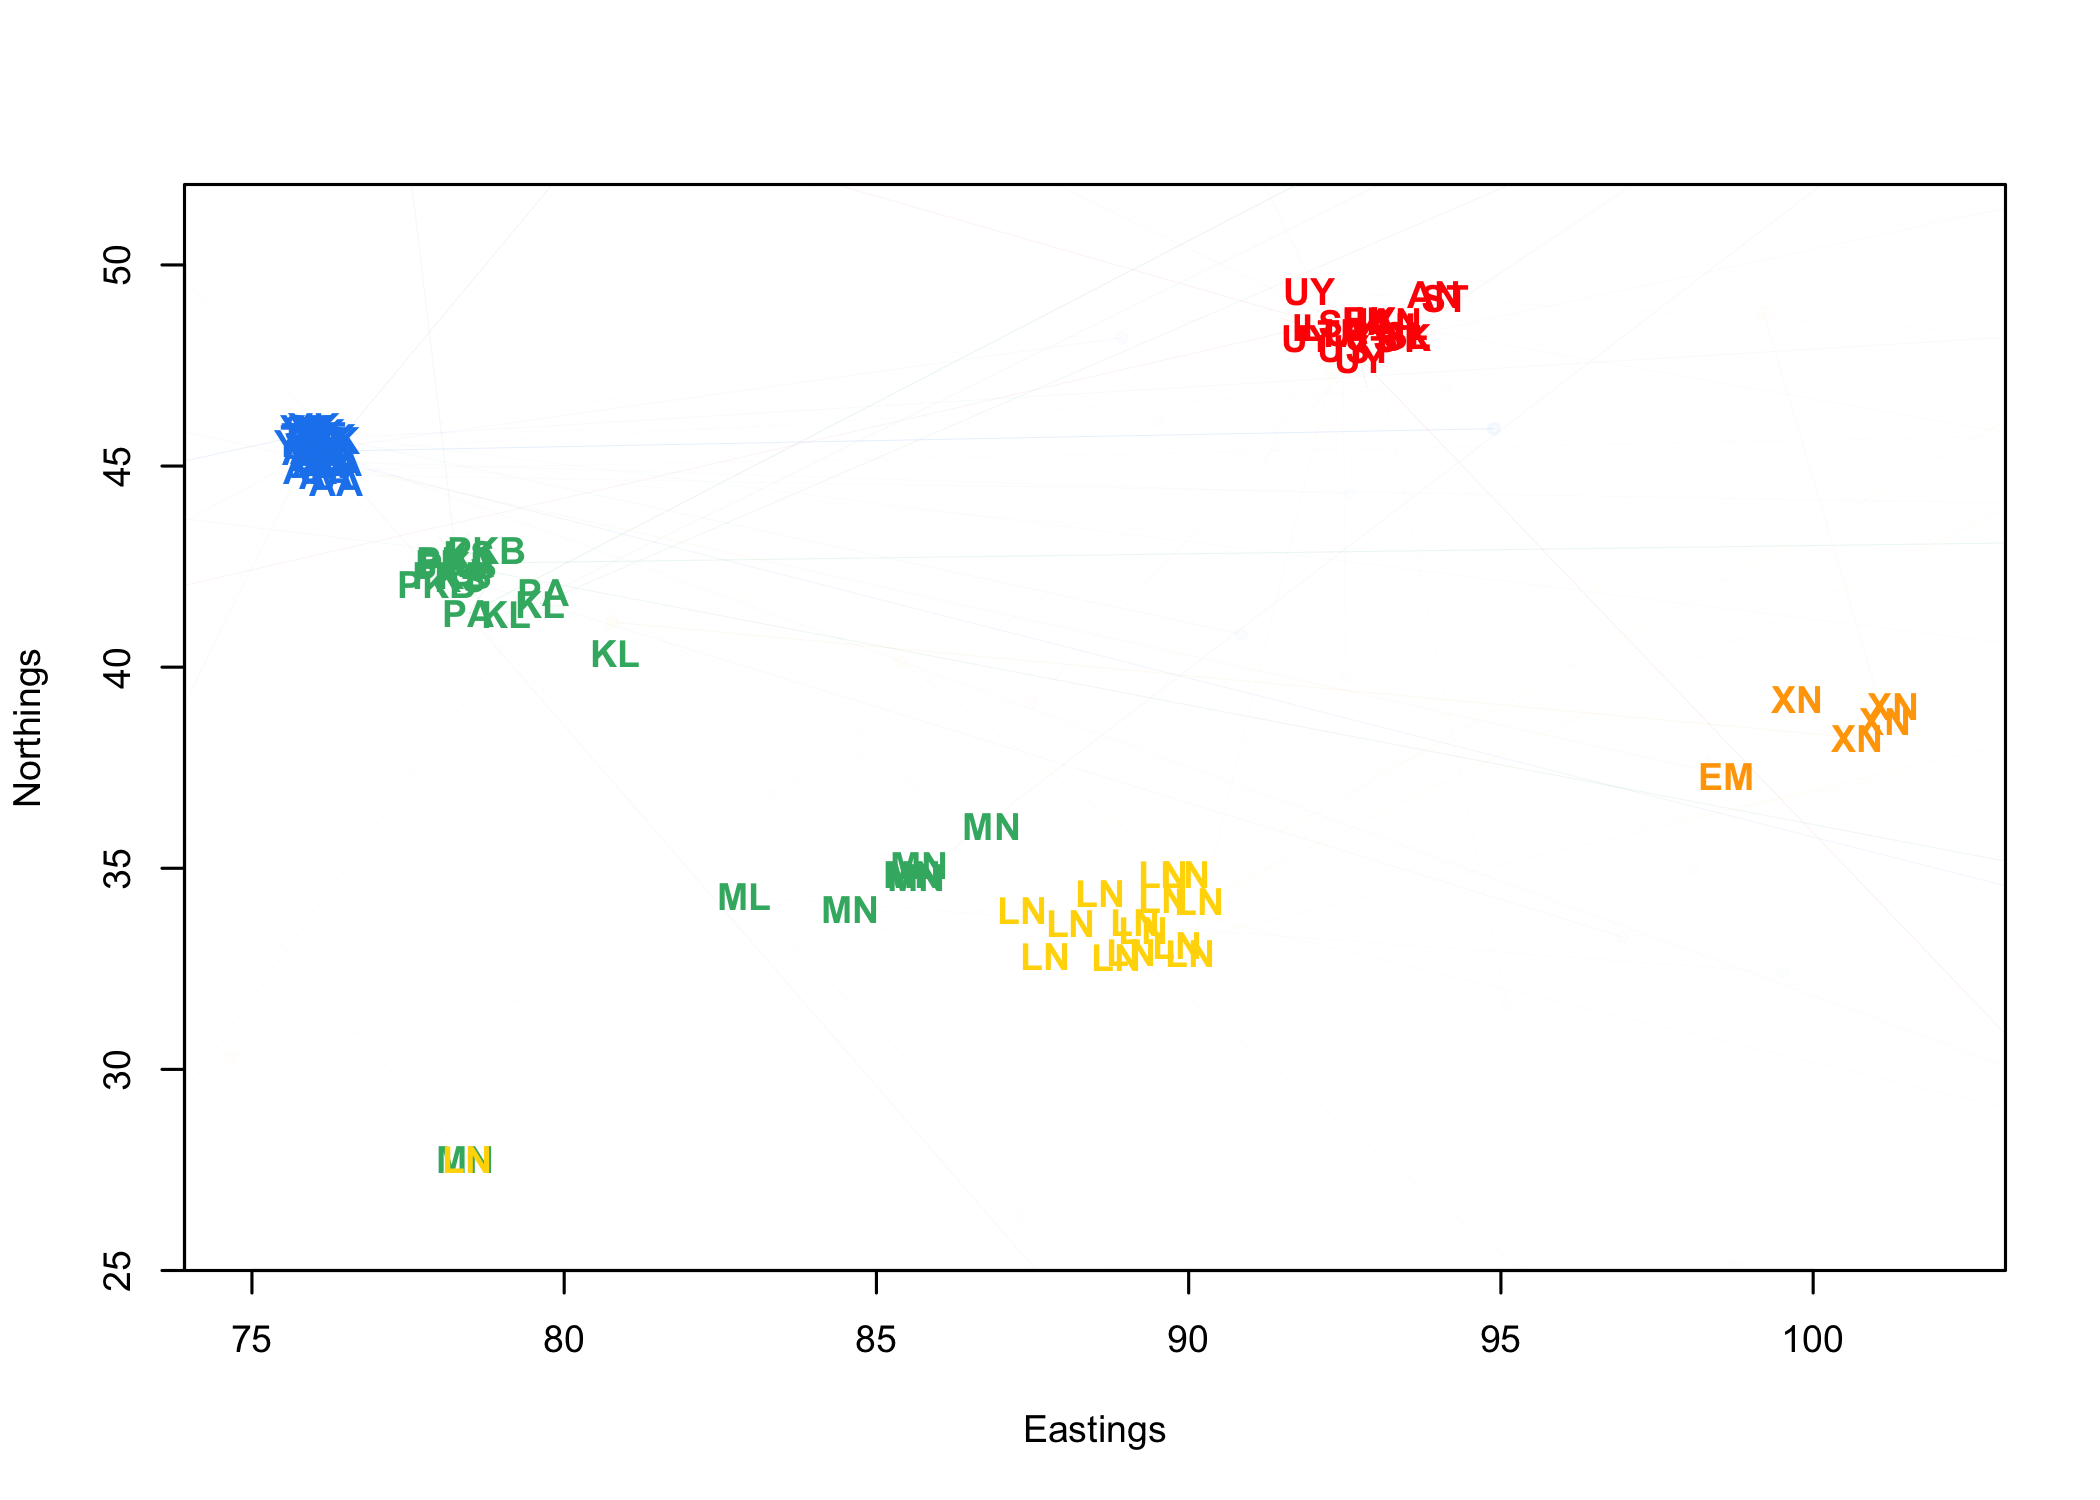
\includegraphics[width=2.8in,height=2.3in]{figs/warblers/individual_warbler_map_arrows_randpr1_closeup.png}}
	\caption{
    Inferred maps for warbler individuals, colored by subspecies in an analysis with admixture inference. 
    \plr{put legend for colors}
    a) map inferred with admixture; b) closeup of all non-\textit{nitrides} samples in the admixture map.
    \plr{labels are hard to read on the right.  This would be better put next to the sample map for comparison?}
}\label{sfig:warbler_ind_maps}
\end{figure}

There are, however, a number of obvious departures in the individual inferred geogenetic map from the population map.  The most obvious is that the location of a pair of \textit{nitidus} samples (in purple) is very far from the rest of the samples.  
These individuals appear to be fairly close relatives:
in the population-level analysis of Figure \ref{sfig:warb_pop_NoAd_nugg},
this increase in shared ancestry was accounted for by a large nugget for the \textit{nitidus} population;
but in the individual-level analysis, they cannot share a nugget parameter, 
and must therefore choose a location close to each other and far from the rest of the samples.
The same phenomenon seems to be at work in determining the locations of a pair of individuals, one identified as \textit{P. t. ludlowi} (Lud-MN3), one as \textit{P. t. trochiloides} (Tro-LN11), 
as they also show an unusually low pairwise sequence divergence see SuppMat Figure \ref{sfig:warb_ind_pwp}).

% There are, however, a number of obvious departures in the individual inferred geogenetic map from the observed map.  The most obvious is that the location of the two \textit{nitidus} samples is very far from the rest of the samples.  
% \gc{Perhaps say colour/location} These individuals appear to be fairly close relatives:
% in the population-level analysis of Figure \ref{sfig:warb_pop_NoAd_nugg},
% this increase in shared ancestry was accounted for by a large nugget for the \textit{nitidus} population;
% but in the individual-level analysis, they cannot share a nugget parameter, 
% and must therefore describe their large amount of shared history by taking locations close to each other and far from the rest of the samples.
% The same phenomenon seems to be at work in determining the locations of a pair of individuals, one identified as \textit{P. t. ludlowi} (Lud-MN3), one as \textit{P. t. trochiloides} (Tro-LN11), 
% \plr{can't tell which these are on the figure.}
% that are very close to one another and also away from the other individuals sampled at their locations. These two individuals show unusually low pairwise sequence divergence (see SuppMat Figure \ref{sfig:warb_ind_pwp}), indicating either recent common ancestry or, potentially, sample contamination.

\plr{
A nice way to check this would be to see where each one of these individuals goes, marginally, with the rest of the locations fixed.
This would be nice because it would also let us demonstrate how to place out-of-sample individuals on the map.
}

The split between \textit{viridanus} and \textit{plumbeitarsus} individuals (blue and red, respectively), in the north at the contact zone of the two waves of expansion, is clearer now than in the population-based analysis, as individuals from the Stolby population have moved to near their respective clusters. 
Despite the fact that \textit{viridanus} and \textit{plumbeitarsus} individuals have moved away from each other in our geogenetic map, 
they are still closer to each other than we would expect if all gene flow between the two was mediated by the southern populations,
in which case we would expect the populations to form a line, 
with \textit{viridanus} at one end and \textit{plumbeitarsus} at the other. 
This horseshoe, with \textit{viridanus} and \textit{plumbeitarsus} at its tips, is steady within and among runs of the MCMC and choice of position priors (see Supplementary Figures \ref{sfig:warb_ind_clouds}\subref{post_map_randpr2}-\ref{sfig:warb_ind_clouds}\subref{post_map_realpr2}).  

%\plr{That's not a horseshoe, that's a triangle, like you'd get from three distinct groups with some intermediates.}

Is this biologically meaningful?  A similar horseshoe shape appears when a principal components (PC) analysis is conducted and individuals are plotted on the first two PCs \citep[see SuppMat Figure \ref{sfig:warb_ind_PC_map} and ][]{alcaide2014genomic}.  
However, as discussed by Novembre \& Stephens (2008) such patterns in PC analysis can arise for somewhat unintuitive reasons. If populations are simulated under a one dimensional stepping stone model, then plotting individuals on the first two PCs results in a horseshoe (e.g.\ see SuppMat Figure \ref{sfig:line_scenario}\subref{line_pops_pca}) not because of gene flow connecting between the tips, but rather because of the orthogonality requirement of PCs (see Novembre \& Stephens for more discussion).  In contrast, when SpaceMix is applied to one dimensional stepping stone data, the placement of samples is consistent with a line (see SuppMat Figures \ref{sfig:line_scenario}\subref{line_pops_post}, \ref{sfig:line_scenario}\subref{line_pops_MAP}). The proximity of \textit{viridanus} and \textit{plumbeitarsus} in geogenetic space may be due to gene flow between the tips of the horseshoe north of the Tibetan Plateau. This conclusion is in agreement with that of \citet{alcaide2014genomic}, who observed evidence of hybridization between \textit{viridanus} and \textit{plumbeitarsus} using assignment methods.


%%%Coop commented this out
%In addition, when we run SpaceMix on the greenish warbler individuals, specifying their location priors to fall along a straight line with samples located at their approximate positions around the horseshoe, the posterior positions of the populations still curl up to form a rough horseshoe (SuppMat Figure \ref{sfig:warb_inds_on_a_line}). 

The SpaceMix map also diverges from the observed map in the distribution of individuals from the subspecies \textit{ludlowi} (in green).  These samples were taken from seven sampling locations along the southwest margin of the Tibetan Plateau, but, in the SpaceMix analysis, they partition into two main clusters, one near the \textit{trochiloides} cluster, and one near the \textit{viridanus} cluster.  This break between samples from the same subspecies, which is concordant with the findings of \citet{alcaide2014genomic}, makes the \textit{ludlowi} cluster unusual compared to the estimated spatial distributions of the other subspecies (see SuppMat Figure \ref{sfig:warb_ind_distcomp}).

\subsection*{Human Populations}
Human population structure is a complex product of the forces of migration and drift acting on both local and global scales, and patterned by geography (Novembre et al 2008 Ralph \& Coop 2013) time (Skoglund et al 2012, 2014), admixture (Hellenthal et al 2014),  landscape and environment (Beall et al 2010, Bigham et al 2010,  Bradburd, Ralph, Coop 2013), and shaped by culture (Reich et al 2009, Atzmon et al 2010, Moorjani et al 2011). To visualize the patterns these processes have induced, we create a geogenetic map for a worldwide sample of modern human populations. In doing so we fully acknowledge that human history at these geographic scales has many aspects that are not well captured by isolation distance or simple admixture models. To simplify the discussion of our results, we talk about samples' locations and those of their sources of admixture, but of course both reflect the compounding of drift and gene flow over many historical processes.  We therefore urge caution in the interpretation our results, and view them as a simplistic but rich visualization of patterns of population structure in humans. 

%Recent work in this area has demonstrated that the signature of these forces can be read in the genomes of modern humans (e.g.\ Novembre et al 2008, Ralph \& Coop 2013, Moorjani, Reich, ARG folks, Hellenthal et al 2014). 

% Specifically, our research questions were: 
% \begin{enumerate}
% \item What is the geography of human population structure?  Which populations cluster with which, and how does the geogenetic map contrast with the observed geography?
% \item Can the map we estimate reconstruct the many of the important expansion events in human pre-history, including the out-of-Africa expansion, the colonizations of Oceania, and the colonization of the Americas via Beringia?
% \item Which human populations are most greatly admixed, and from where?  Will the SpaceMix results confirm the admixture findings of previous studies?
% \end{enumerate}

%To answer these questions,

We used a random subset of 10,000 SNPs from the SNP dataset of \citet{Hellenthal}, which is comprised of 1,490 individuals sampled from 95 populations (see Fig.\ \ref{sfig:empirical_maps}\subref{human_map} for map of sampling), as well as the latitude and longitude attributed to each population.  We ran two sets of SpaceMix analyses: in the first, we estimated population sample locations, and in the second, we 
also allowed admixture. We note that few of the putative admixture events that we report have escaped the notice of previous investigators, which is unsurprising given the depth of recent attention on human admixture studies, particularly on the subset of HGDP samples \citep[see ][for various global analyses]{rosenberg_genetic_2002,li_worldwide_2008,Loh:13,patterson_ancient_2012,Hellenthal}. However, what is novel is the ability to vizualize these admixture events in a geographic context, and that these admixture signals stand out against a null model of isolation by distance (rather than tree-based models).

%Populations generally cluster with other populations sampled on their continent, and the relative placement of populations is similar to that of their observed geography.  Sub-Saharan African populations are distributed in a manner consistent with their sampled latitude, with the San populations in the South and the Ethiopian populations closest to the Eurasian populations in the North.  North African populations, such as the Moroccan, Tunisian, and Egyptian populations, cluster with Middle Eastern populations such as the Yemeni and the UAE, and are quite close to both the Ethiopian populations and the western European populations, such as the Sicilians, the Cypriots, the Tuscans, and the Sardinians.

When population samples choose only their own locations, the map roughly recapitulates the geography of the samples (Fig.\ \ref{sfig:globe_noad_maps}). This nicely holds also zooming in on the more heavily sampled area of Eurasia (Fig.\ \ref{sfig:globe_noad_maps}). We see that both the populations in the Americas and those in Oceania cluster close to the East Asian populations, but that the two clusters are on opposite sides.  The proximity of these groups to the East Asians represents the fact that both groups share an ancestral population in the relatively recent past with East Eurasian populations, but the two expansions occurred independently. As in our simulations (Figure \ref{sfig:expansion_scenarios}\subref{expansion_inference}) population expansions/bottlenecks have distort the relationship between geographic and geogenetic distance. In the SpaceMix analysis of the human genetic data, the scale of inferred inter-population distance within Africa is much greater than that between any other group (see SuppMat Fig.\ \ref{sfig:globe_noad_distcomp}), and the slope of the relationship between observed and estimated geographic distances between populations on each continent decays with distance from Africa.  This pattern is consistent with a history of human colonization events characterized by serial bottlenecks \citep{Harpending_Rogers_2000,prugnolle_geography_2005,Ramachandran:05} and other models \citep{pickrell_reich:14} following out-of-Africa expansion, a subsequent expansions into Western Eurasia, East Asia, the Americas, and Oceania. 

\begin{figure}
	\centering
		\subcaptionbox{Inferred map of human populations \label{globe_all_noad_map}}
			{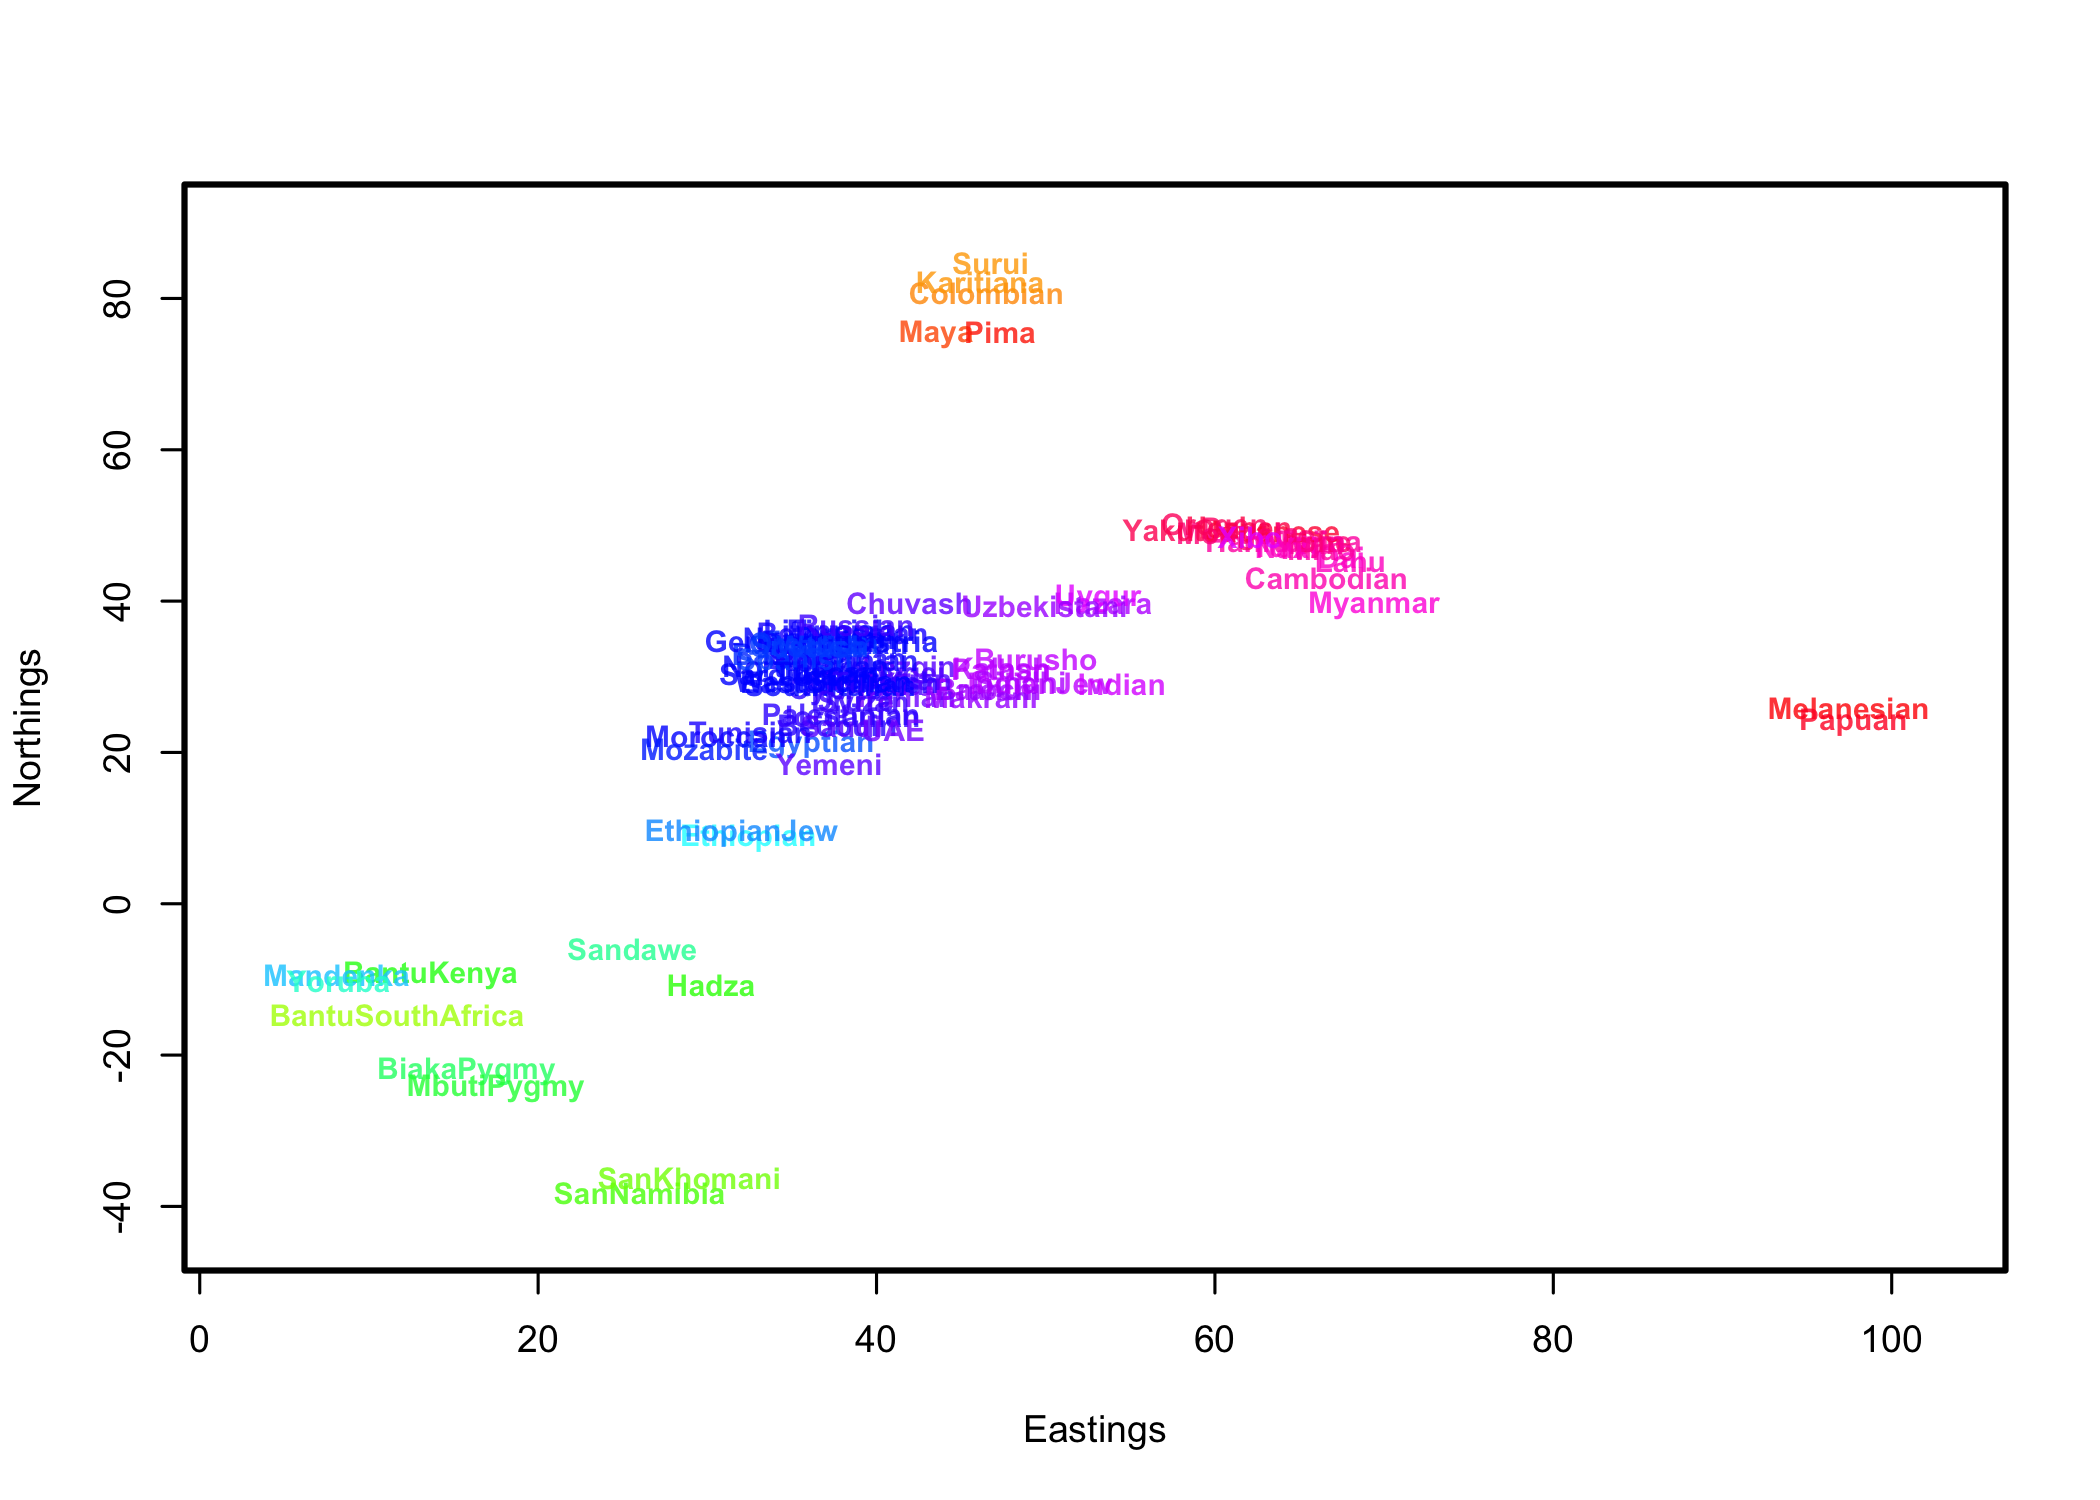
\includegraphics[width=2.8in,height=2.3in]{figs/globetrotter/globe_NoAd_map.png}}
		\subcaptionbox{Closeup of Eurasian populations \label{globe_eurasia_noad_map}}
			{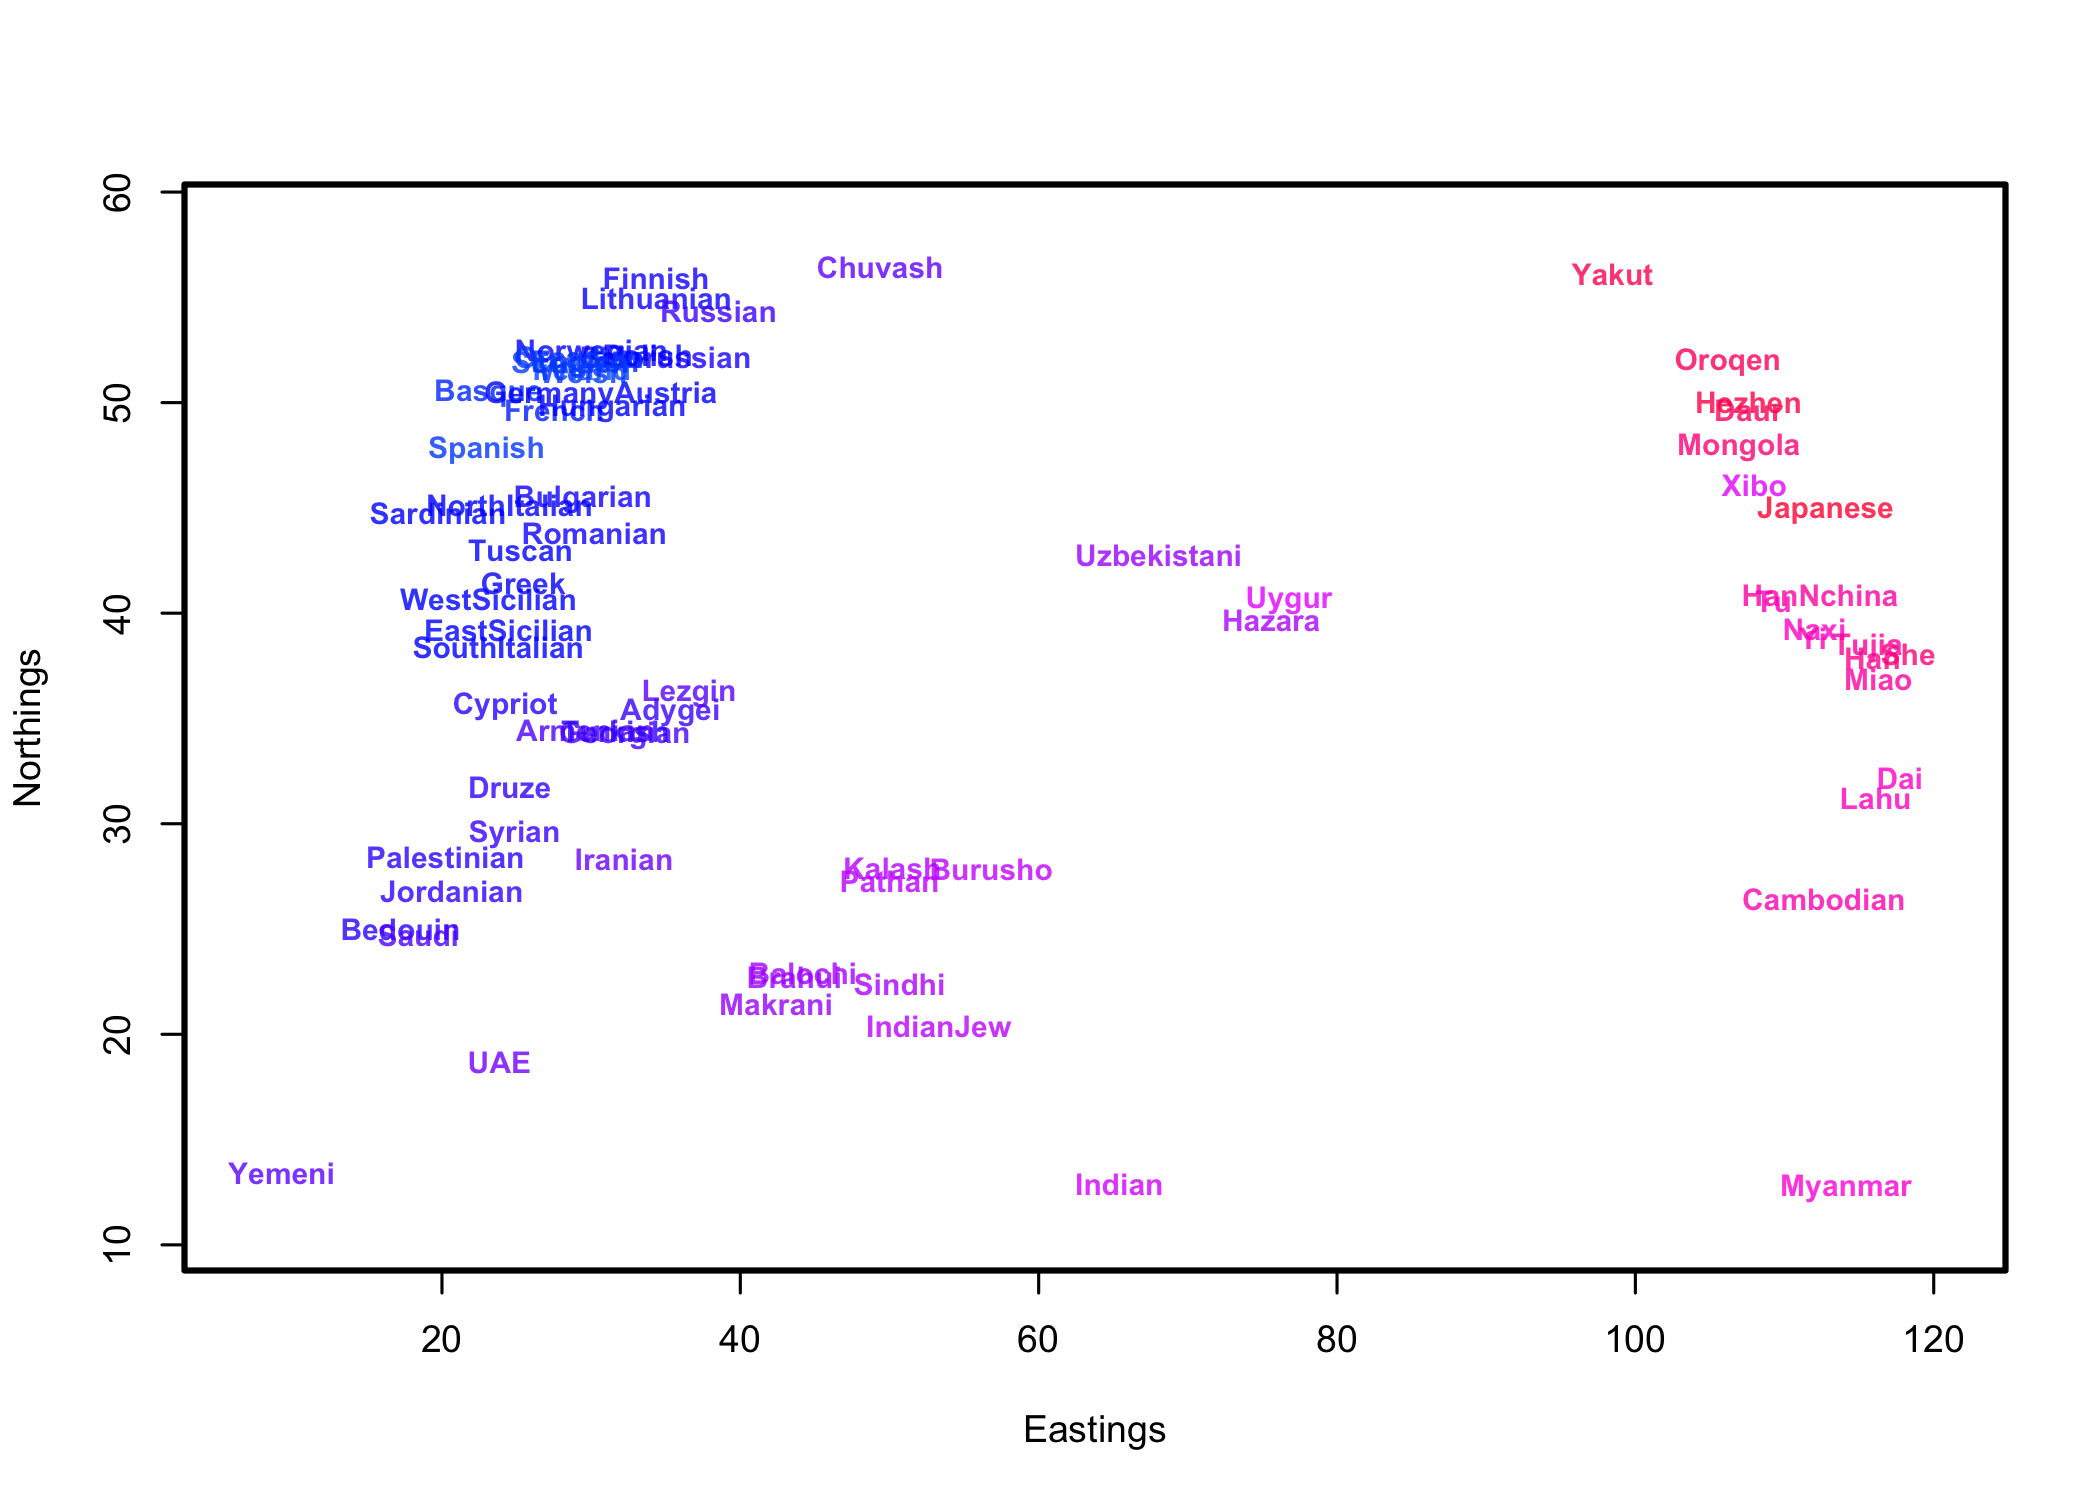
\includegraphics[width=2.8in,height=2.3in]{figs/globetrotter/globe_Eurasia_NoAd_map_indproc.png}}
	\caption{Map of human populations, inferred without admixture. (a) complete map; (b) close up of Eurasian 
populations.}\label{sfig:globe_noad_maps}
%(b) close up African populations; (c) close up of all non-African populations;
\end{figure}

%We recover evidence for several major population expansions and colonization routes in human pre-history.  
%\plrm{``observed pairwise'' should be ``geographic'', here and elsewhere?}



%We can see evidence of these expansions by examining the relationship between observed and estimated pairwise distance between the daughter populations of a putative expansion event.   As can be seen in Figure \ref{sfig:expansion_scenarios}\subref{expansion_inference}, populations that have recently expanded on the landscape are less differentiated both from each other and from their parent population than would be expected from their geographic separation, and this fact is reflected in the decreased ratio between estimated and observed pairwise distances between members of an expansion event.


%\plr{Here the discussion sounds like by default, we'd expect these very different discrete groups, so that placement between them is recent admixture.  That would be true if most modern populations came from one of a few recent expansions.  A different prior would be that populations be uniformly distrubted, making the intermediate popluations expected, and the clustering something to explain.}
%We also see intriguing evidence for potential admixture in the placement of the Chuvash, Uzbekistani, Hazara, and Uygur populations, which choose locations intermediate between Europe and East Asia.  Notably, the Xibo who are sampled from a geographic location close to the Uygur, choose a geogenetic location within the East Asian samples.  The placement of the Moroccan, Mozabite, and Ethiopian populations, which choose locations between the western Eurasian cluster and the African cluster, is also suggestive of potential admixture.  

To investigate possible patterns of admixture further, we ran a SpaceMix analysis with admixture (results shown in Figure \ref{sfig:globe_ad_maps}). The biggest change between the geogenetic map of human populations inferred with admixture and that without is the positioning of African samples with respect to the rest of the world.  The relatively large geogenetic distances between these groups reflects the fact that Eurasian, North African, Oceanian, and American populations all share relatively large amounts of drift not shared with the Sub-Saharan African samples. The inclusion of admixture allows samples that fall intermediate between Sub-Saharan Africa and North Africa and the Middle East to move closer to one or the other, which, in turn, allows each of those major clusters to move relatively farther apart.  The Ethiopian and Ethiopian Jewish samples move to be closer to the Sub-Saharan samples than the of the North African samples, but draw substantial amounts of admixture ($\sim 40\%$) from close to where the Egyptian sample has positioned itself in the the Middle East cluster, as do the Sandawe \citep{hodgson_early_2014,Pickrell:12}. The SanKhomani draw admixture from near Syria, which may reflect multiple distinct geographic sources of admixture as discussed by \citep{Hellenthal} and \citep{Pickrell:14}. 
Interestingly the Bantu South African sample, though it moves to join the other Bantu sampless, draws admixture from close to the San populations. This is consistent with previous signals of the expansion of Bantu-speaking peoples into southern Africa  \citep{Pickrell:12,Jakobsson_genomic_2012,Pickrell:14,Hellenthal}. 

The majority of North African sampless (Egyptian, Tunisian, Morocan, Mozabite) move to join the Middle Eastern samples (positioning in rough accord with their sampling location along North Africa), and draw admixture from near the Ethiopian samples. All of the Middle Eastern samples draw admixture from close to the location chosen by the Ethiopian samples and where most of North African samples draw admixture from, representing the complex history of North African--Middle Eastern gene flow \citep{henn_genomic_2012,Hellenthal}. 


%%%%%%%%%
%Now instead of occupying an intermediate position the two Ethiopian samples draw a substantial proportion of their ancestry ($\sim 40\%$) from close to where the Egyptian sample has positioned itself in the the middle East cluster. The Sandawe population also draw a substantial portion of their ancestry from the middle east cluster.  Where's the Hadza going? Reciprocally, our North African samples (Egyptian, Tunisian, Morocan, Mozabite), having moved to join the middle eastern populations draw ancestry from close to the Ethiopian samples. 

%Hellenthal et al infer 2 admixture events and 3 admixture sources for the San Khomani: 1 event from the Bantu peoples in South Africa, and 1 event from a combination of northern European and southeast Asian populations.  

A number of other populations draw admixture from Africa. The Sindhi, Makrani, and Brahui draw admixture from close to the location of the Bantu samples \citep{Hellenthal}, and the Balochi and Kalash draw admixture from some distance away from African populations.  Of the European samples, the Spanish and the East and West Sicilian samples all draw small amounts of admixture from close the Ethiopian samples presumably reflecting a North African ancestry component \citep{moorjani_history_2011,botigue_gene_2013}. 

The other dominant signal of admixture is between East and West Eurasia \citep[a signal documented by many authors][]{rosenberg_genetic_2002,li_worldwide_2008, xu_genome-wide_2008,Hellenthal}. The majority of samples maintain their relative positions within each of these groups; however, several of the populations that chose locations intermediate between eastern and western Eurasia now move towards one side, and draw admixture from the other.  The Uzbekistani and Hazara samples move to be closer to the East Asian samples, while drawing a substantial admixture proportion from close to where the Georgian and Armenian samples have located themselves, while conversely the Uygur sample moves to be close to the Burusho, Kalash, and Pathan samples. The Tu sample (who locate to East Asia) draw a small amount of ancestry from close to where the Uygur have positioned themselves. The Chuvash move close to Russian and Lithuanian samples, drawing admixture from close to the Yakut; the Turkish sample also draws a smaller amount of admixture from here. There are a number of other East-West connections: the Russian, Adygei samples have admixture from a location ``north'' of our East Asian samples, and Cambodia draws admixture from close to the Eygptian sample \citep{Treemix, Hellenthal}. 

%\plrm{could be recent, colonial-era admixture? \href{http://en.wikipedia.org/wiki/Indian_diaspora_in_Southeast_Africa} someone would have probably noticed this, though...}

There are a number of samples that draw admixture from locations that are not immediately interpretable.  For example, the Hadza and Bantu Kenyan samples draw admixture from somewhat close to India, 
and the Xibo and Yakut from close to ``northwest'' of Europe.  
The Pathan samples draw admixture from a location far from any other samples' locations, but close to where the India samples also draws admixture from. 
The Myanmar and the Burusho samples both draw admixture far from the locations estimated for other samples as well.% check Indian Jew

%\plrm{should be careful: the Pathan live in India; find a different name for ``India'' sample?} G: The Pathan samples are from Pakistan

There are a number of possible explanations for these results. As we only allow a single admixture arrow for each sample, populations with multiple, geographically distinct, sources of admixture may be choosing admixture locations that average over the sources. This may be the case for the Hadza and Bantu Keynan samples.  A second possibility is that the relatively harsh prior on admixture proportion forces samples to choose lower proportions of admixture from locations that overshoot their true sources; this may explain the Xibo and Yakut admixture locations. A final explanation is that good proxies for the sources of admixture may not be included in our sampling, either because of of the limited geographic sampling of current day populations, or because of old admixture events from populations that are no long extant. The admixture into the Indian and Pathan samples (whose admixture source also clusters with the Indian Jew samples in some MCMC runs) may be an example of this, as \citet{reich_india_2009,moorjani_india_2013} have hypothesized that many populations from the Indian subcontinent may be descended from an admixture event involving an ancestral Southern Indian population not well-represented by our samples. 

In the Supplementary Figures XXXX-ZZZZZ we show the results of other independent MCMC analyses on these data. The broad-scale patterns and results discussed above are consistent across these runs. However, as is to be expected, there is significant heterogeneity in the exact layout of sample and admixture locations. For example, there is some play, among MCMC runs, in the internal orientation of the African locations with respect to Eurasia.  Samples that draw a significant amount of admixture, such the central Asian populations (Uygur, Hazara and Uzibeckistani), switch their locations with that of their source of admixture (as was also seen across MCMC runs in the warbler data analysis). Similarly the Ethiopian and Ethiopian Jews choose locations, in some MCMC runs, close to the other North African samples, and draw admixture from near the Sub-Saharan samples (as do the other North African samples).
\plrm{right, so are figures a sample from the posterior? If so, should say was chosen how?}

\begin{figure}
	\centering
		\subcaptionbox{Inferred map of human populations \label{globe_all_ad_map}}
			{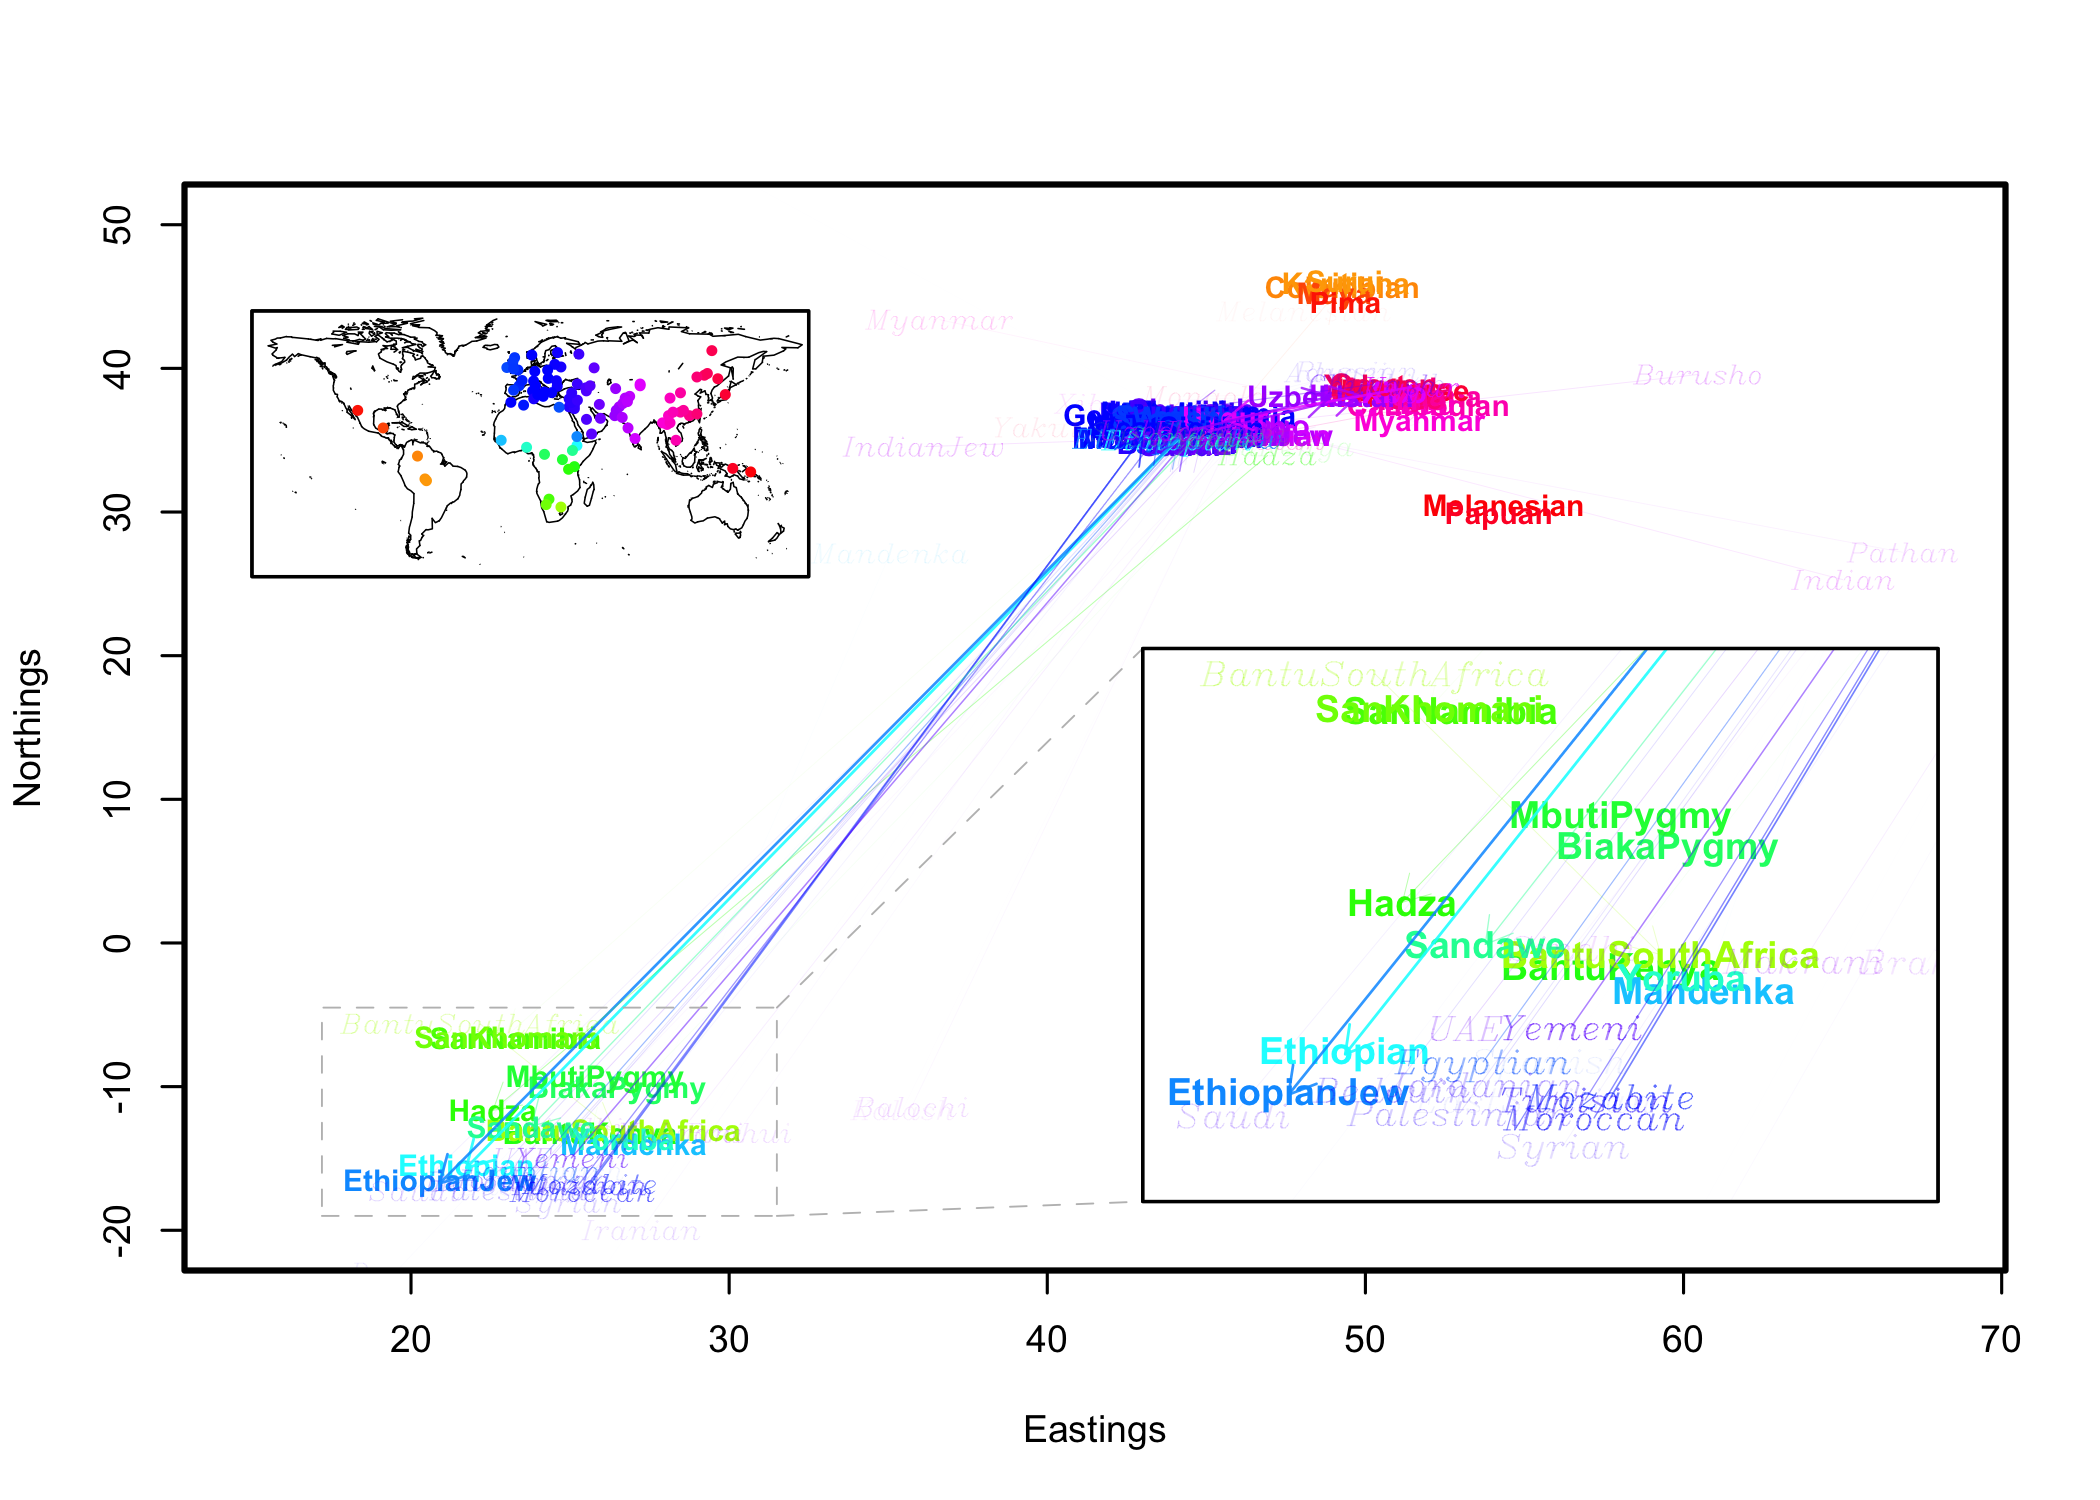
\includegraphics[width=2.8in,height=2.3in]{figs/globetrotter/globe_Ad_map_AfricaInset.png}}
		\subcaptionbox{Closeup of Eurasian populations \label{globe_eurasia_ad_map}}
			{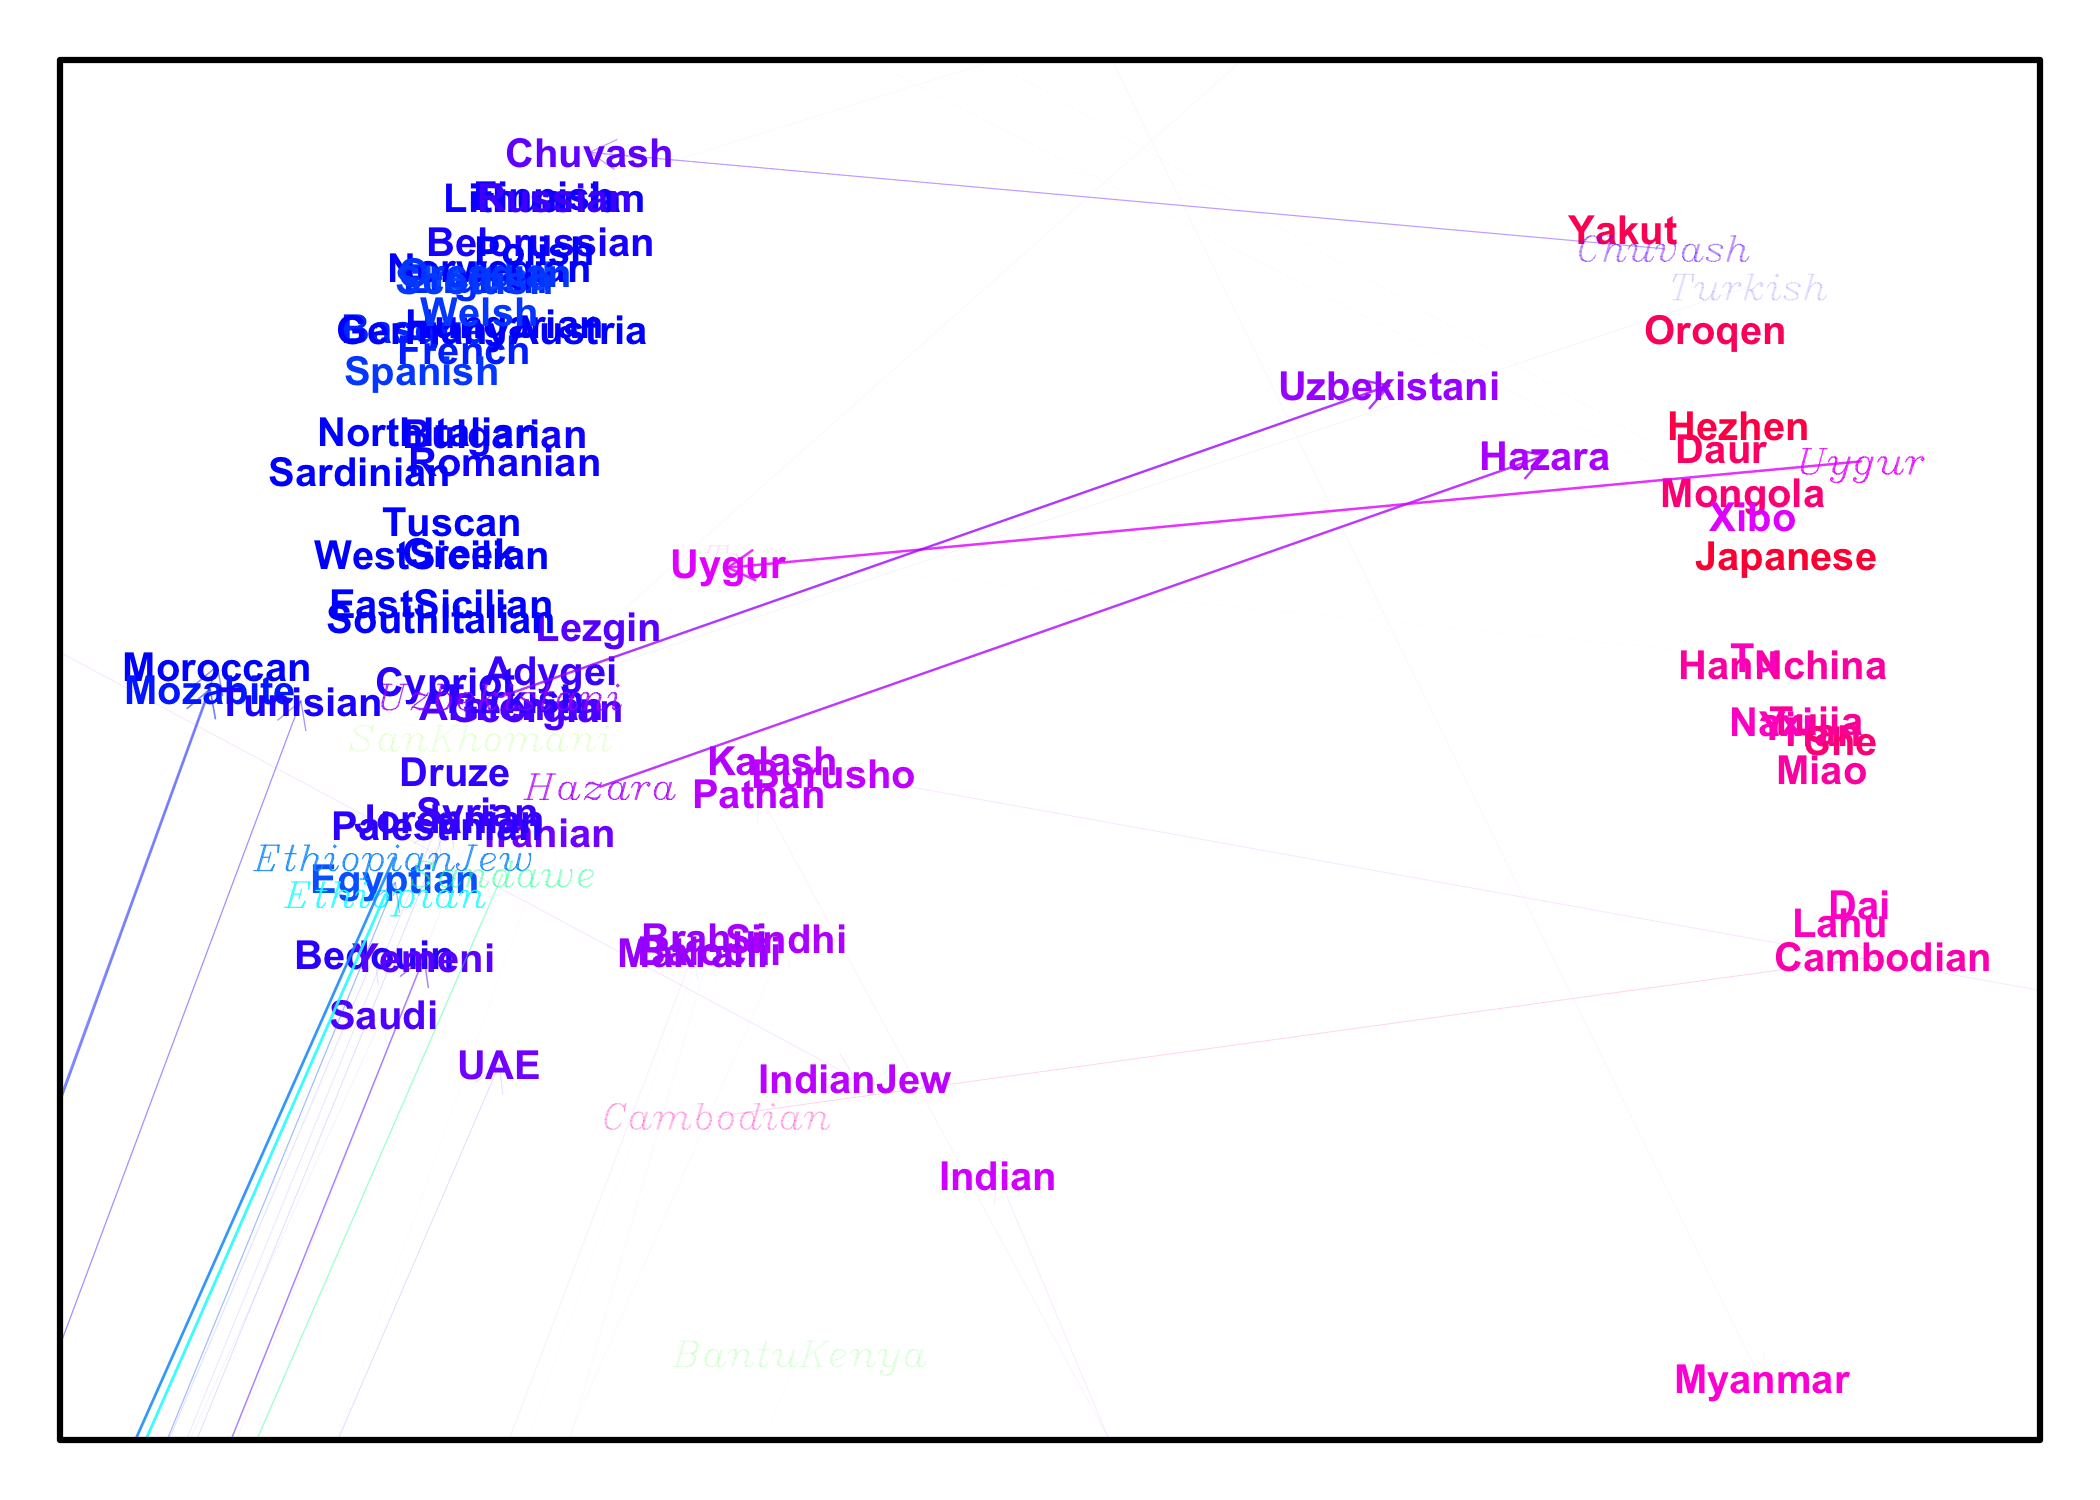
\includegraphics[width=2.8in,height=2.3in]{figs/globetrotter/eurasia_Ad_map_indproc.png}}
		\subcaptionbox{Inferred admixture proportions for human populations \label{globe_ad_props}}
			{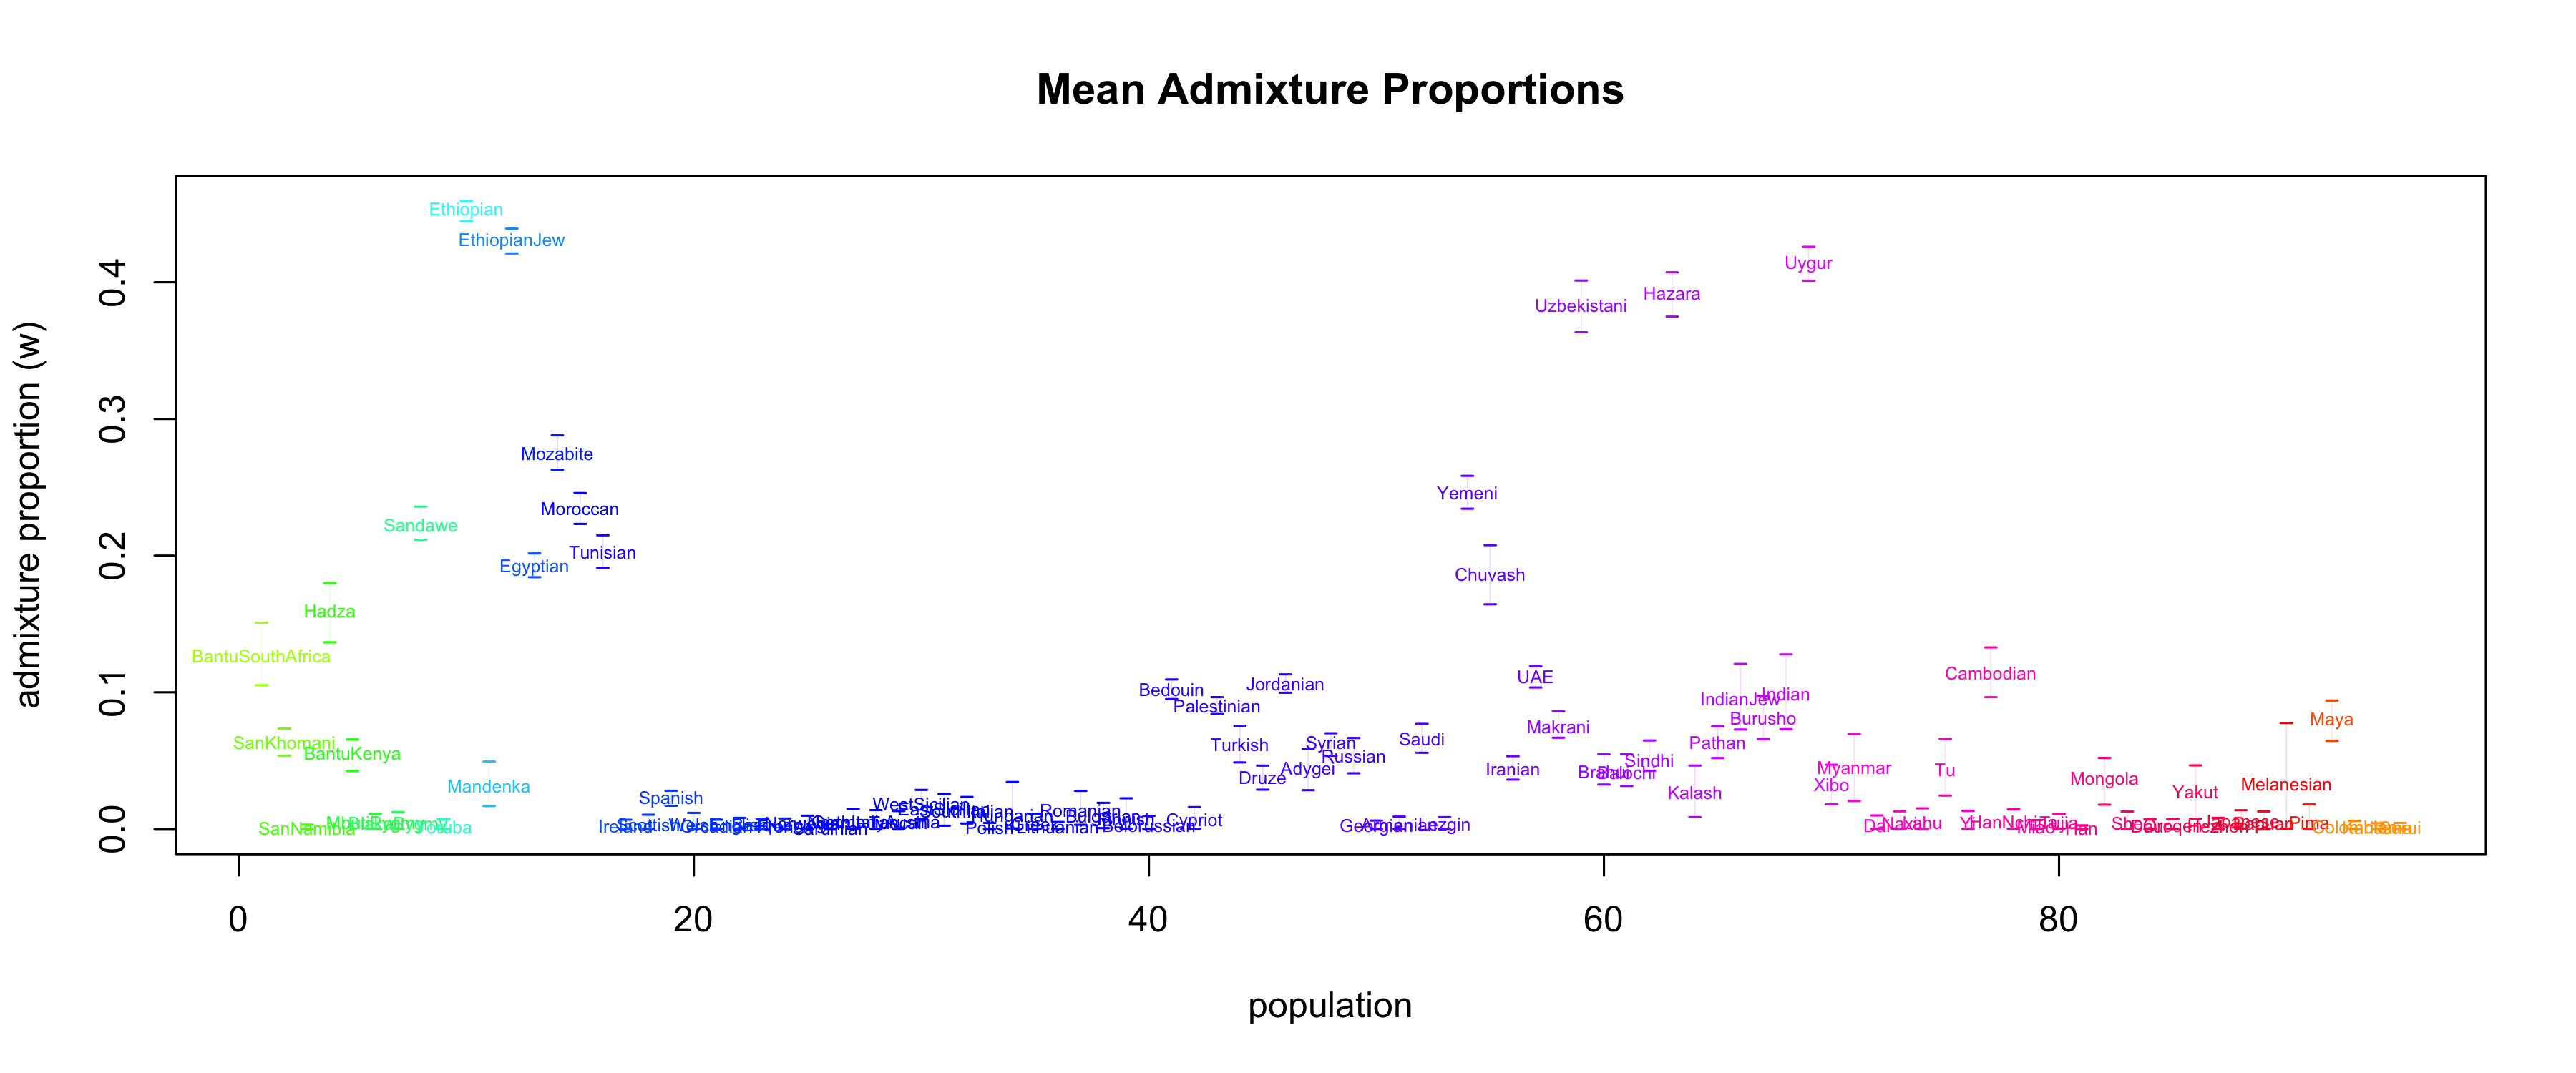
\includegraphics[width=5.6in,height=2.33in]{figs/globetrotter/globe_Ad_proportions.png}}
	\caption{Map of human populations, inferred with admixture. (a) complete map; (b) close up of Eurasian populations; c) mean admixture proportions for each population}\label{sfig:globe_ad_maps}
\end{figure}

%\plr{I might not list the f-stats here; as they aren't really ``model-based inference for population relationships''.}

%Graham wasn't sure what this meant: SpaceMix, unlike methods such as STRUCTURE or Geneland, does not infer hierarchical population structure, but it can be used as a useful guide in those analyses.
%Within the constellation of existing methods for inferring and illustrating patterns of population structure, SpaceMix falls between methods that use model-based inference to infer population trees, such as TreeMix, mixmapper, or Reich et al's \textit{f}-statistics, and methods that use dimensionality reduction to visualize patterns of structure on a map.  SpaceMix, unlike methods such as STRUCTURE or Geneland, does not assume hierarchical population structure. %, but it can be used as a useful guide in those analyses.


%%%%%%%% %%%%%%%%%%%%
\subsection*{Discussion}

The patterns of genetic variation observed in modern populations are the product of a complex history of demographic processes.  We choose to model those patterns as the outcome of a spatial process with geographically determined migration,
and we have included statistical elements to accommodate deviations from spatial expectations.
However, the true history of a sample of real individuals is vastly more complex than any low-dimensional summary,
and, as with any summary of population genetic data, 
SpaceMix results should be interpreted with this in mind.
Furthermore, our ``admixture'' events are shorthands for demographic relationships
that occurred over possibly substantial lengths of time and regions of the globe;
approximating this by a single point in space is certainly an oversimplification.
Aspects of population history that are better described as a population phylogeny may be difficult to interpret using SpaceMix,
and may be better suited to visualization with hierarchical clustering-based methods \citep{STRUCTURE} or TreeMix/Mixmapper-like methods \citep{Treemix,lipson_mixmapper_2013}.  
There is obviously no one best approach to studying and visualization population structure;
investigators should employ a range of appropriate methods to identify those that provide useful insight. 
%\gc{this prolly needs to be less preachy}

%\plr{
%How about a paragraph summarizing the advantages over PCA and structure up here?  
%Structure: we make maps.  
%PCA: we allow admixture and are not constrained to linear relationships between allele and location.
%With four populations in a line, if drift is sufficently stronger than migration,
%PCA will use three PCs to separate them, and will put them at the corners of a tetrahedron;
%SpaceMix should get the linear arrangement right.
%This is related to the triangular configuration seen in the warblers.
%}

SpaceMix offers much of the flexibility of PCA - like PCA, is well suited to describing population structure in a continuous fashion - 
but it also has a number of advantages over PCA. 
When isolation by distance holds, the first (one or) two PCs often correspond to some simple rotation of latitude and longitude; 
however, these first two PCs explain a relatively small part of the total variance of the data. 
Due to the linearity of PCs, many higher order PCs 
have to correspond to higher order functions of positional information under isolation by distance, 
and are therefore needed to explain the bulk of the variance \citep{novembre_interpreting_2008}. 
These higher order PCs can be hard to interpret in empirical data (see discussion in the warbler section).

In comparison, if isolation by distance holds then (nearly) all of the variance will be captured by SpaceMix in the inferred geogenetic positions 
(to the extent to which the parametric form of the covariance is flexible enough to capture the empirical decay of covariance with distance). 
The recently introduced SPA approach \citep{yang_model-based_2012} also has this advantage, 
but only really makes use of loci that conform to particular spatial patterns,
so it is making use of less of the data and is less flexible 
(although we note that PCA and SPA both have significant speed advantages over SpaceMix).  
The application of SpaceMix to humans nicely illustrates the utility of our approach: 
the first two PCs of this dataset resemble a boomerang (SuppMat Figure XXX), 
with its arms corresponding to the Africa/Non-Africa split and the spread of populations across Eurasia. 
In contrast, while the SpaceMix geogenetic map is dominated by the out of Africa drift, 
it also captures much more detail than is contained in the first two PCs (ref Eurasia figure).
This comparison is also nicely illustrated by the example in SuppMat Figure \ref{sfig:line_scenario}.

An advantage of PCA is that it can explain more complex patterns of population structure by allowing up to $K$ different axes.
Although SpaceMix can easily be extended to more than two dimensions, 
simply by allowing $G_i$ to describe the location of a sample in $d$ dimensions, 
the interpretation and visualization of these higher dimensions would prove difficult, 
and so for the moment we stick with two dimensions.

%(by, e.g., estimating population locations, allowing population-specific drift effects in the nugget parameters, and allowing the inference of admixture), 
%\plr{I wouldn't put ``estimating locations'' here -- we don't expect the map to look just like geography.  if it did, we wouldn't need the method, since we already have that map.}

Another strong advantage of SpaceMix over current methods is the introduction of admixture arrows. 
Although PCA can be interpreted in light of simple admixture events \citep{mcvean_genealogical_2009}, 
and \citet{yang_model-based_2012,yang_spatial_2014} can locate the recent, spatially admixed ancestry of out of sample individuals,
neither approach explicitly models admixture between multiple geographically distant locations,
as SpaceMix does.
Assignment methods are designed to deal with many admixed samples \citep{STRUCTURE}, 
but they have no null spatial model for testing admixture.
We feel that an isolation by distance null model is often a more appropriate for testing for admixture, 
especially when there is geographically dense sampling. 
SpaceMix offers a useful tool to understand and visualize spatial patterns of genetic relatedness when many samples are admixed. 

As currently implemented, SpaceMix allows each population to have only a single source of admixture, 
but some modern populations draw substantial proportions of their ancestry from more than two geographically distant regions.
In such cases the inferred source of admixture may fall between the true locations of the parental populations.  
Although it is statistically and computationally possible to allow each population to choose more than one source of admixture, 
we were concerned about both the identifiability and the interpretability of such a model, and have not implemented it.
However, there may be empirical datasets in which such a modeling scheme is required to effectively map patterns of population structure.
In addition, we have assumed that only single populations are admixed, when in fact it is likely that particular admixture events may affect multiple samples.

One concern is that the multiple admixed samples (from a single admixture event) may simply choose to cluster close to each other, 
and not need to draw admixture from elsewhere due to the fact that their frequencies are well described by their proximity to other admixed populations.  
Along these lines, it is noticeable that many of our European samples draw little admixture from elsewhere \citep[a fact also noted by][ using a different approach]{Hellenthal}, 
despite evidence of substantial admixture \citep{lazaridis_ancient_2014}.
This may reflect the fact that all of the European samples are affected by the admixture events, and are relatively over-represented in our sample. 
However, this may also simply reflect the fact that the admixture is ancient, 
and the ancient individuals used as proxy sources of these events are not well represented by our extant sampling. 
Reassuringly, we see multiple cases where similarly admixed populations (Central Asians, Middle Eastern and North African) 
populations are separately identified as admixed. 
This suggests that geogenetic clustering (in lieu of drawing admixture) of populations that share similar histories of admixture is not a huge concern 
(at least in some cases). 
The method could in theory be modified to allow geogenetically proximal populations to draw from the same admixture event;
however, this may be difficult to make fully automated.

%Three factors in particular stand out as potential sources of difficulty for the model.  %The first is that there may be empirical datasets for which the assumption of isolation by distance is inappropriate.  

%In taxa that migrate from their sampled locations and breed more or less panmictically elsewhere,
%or for some broadcast spawners, 
%a geogenetic map inferred by SpaceMix may bear no relation to the observed sample locations, and thus may be difficult to parse.  However, cases in which there is little or no concordance between the observed and inferred geography may also prove the most interesting and informative.

In this paper we have focused on the covariance among alleles at the same locus, 
but linkage disequilibrium (LD; covariance of alleles among loci) 
holds rich information about the timing and source of admixture events \citep[e.g.][]{chakraborty_admixture_1988,moorjani_india_2013, Hellenthal,gravel_population_2012} 
as well as information about isolation by distance \citep{ralph_geography_2013}.
Just as population graph approaches have been extended to incorporate information from LD \citep{Loh:13}, 
a spatial covariance approach could be informed by LD. 
A null model inspired by models of LD under isolation by distance models \citep{blah} could be fitted, 
allowing the covariance among alleles to decay with their geographic distance and the recombination distance between the loci. 
In such a framework, sources and time-scales of admixture could be identified through unusually long-distance LD between geographically separated populations. 

The landscape of allele frequencies on which the location of the samples, 
and those of the sources of admixture for the sampled populations, 
are estimated is entirely informed by the placement of other modern samples.  
This immediately leads to the caveat that, instead of ``location of the parental population,''
we should refer to the ``location of the closest descendants of the parental population.''
The increased sequencing of ancient DNA \citep[see ][for a recent review]{pickrell_reich:14} promises an interesting way forward on that front,
and it will also be exciting to learn where ancient individuals fall on modern maps, 
as well as how the inclusion of ancient individuals changes the configuration of those maps \citep{skoglund_investigating_2014}..
The inclusion of ancient DNA samples in the analyzed sample offers a way to get better representation of the ancestral populations from which the ancestors of modern samples received their admixture.  
However, it is also possible to model genetic drift as a spatiotemporal Gaussian process, 
in which covariance in allele frequencies decays with distance in both space and in time.  
We are currently exploring using ancient DNA samples as  `fossil calibrations' on allele frequency landscapes at points in the past, 
so that modern day samples may draw admixture from coordinates estimated in space-time.

\section*{Conclusion}
In this paper we have presented a statistical framework for modeling the geography of population structure from genomic sequencing data.
We have demonstrated that the method, SpaceMix, is able to accurately present patterns of population structure in a variety of simulated scenarios, which included the effects of spatially heterogeneous migration, population expansion, and population admixture.  In our empirical applications of SpaceMix, we have largely recovered previously estimated population relationships in a circum-Tibetan sample of greenish warblers and in a global sample of human populations, while also providing a novel way to depict these relationships.  The geogenetic maps SpaceMix generates serve as simple, intuitive, and powerful summaries of patterns of population structure. 
SpaceMix combines the advantages of other methods for inferring and illustrating patterns of population structure, 
using both model-based inference to infer population relationships (like TreeMix and mixmapper), 
and producing powerful visualizations of genetic structure on a map (like PCA, SPA).

%\section*{Future Directions}

%As noted in the third caveat above, the ancestral populations that have donated to the genetic makeup of modern day samples will not be among the samples in the current analysis, and therefore the inferred geography of admixture may only coarsely approximate the truth (depending on the complexity of the demographic history and the extent to which daughter populations of that ancestral admixture source both resemble their parents and have stayed put, geographically).  The inclusion of ancient DNA samples in the analyzed sample offers an intriguing way forward in getting better representation of the ancestral populations from which the ancestors of modern samples received their admixture.  However, it is also possible to model genetic drift as a spatiotemporal Gaussian process, in which covariance in allele frequencies decays with distance both in space and in time.  In this model, which we are currently developing, ancient DNA samples can `calibrate' allele frequency landscapes at points in the past, and modern day samples may draw admixture from estimated coordinates in space-time.

\newpage

\section*{Methods}
As described above, we have developed an algorithm, called SpaceMix, that uses the standardized sample allele frequency covariance and the the likelihood equation in equation \eqref{eq:admixed_post_prob} to simultaneously estimate the posterior distribution of the population locations, $G$, their sources of admixture, $\identifyadmixsource{G}$, their admixture proportions, $w$, their independent drift parameters, $\eta$, and the parameters of the model of isolation by distance, $\vec{\alpha}$.  The inference procedure has two main components: (1) the derivation of the standardized sample allele frequency covariance matrix, and (2) a Markov chain Monte Carlo algorithm that samples parameter values from the posterior distribution.  Here, we describe these procedures in detail.

\subsection*{Deriving the standardized sample covariance}

We assume that the sample allele frequencies at locus $\ell$ across populations are given by
%
\begin{equation}
\hat{f}_{\ell} \sim MVN(\epsilon_{\ell}, \epsilon_{\ell} (1-\epsilon_{\ell})\Omega)
\end{equation}
%
where $\Omega$ is the covariance matrix that describes shared population history between populations, $\epsilon_{\ell}$ is the ancestral mean frequency at that locus, and $\epsilon_{\ell}(1 - \epsilon_{\ell})  \frac{1}{\bar{S}}$ on the diagonal of the covariance matrix captures, to first approximation, the effects of sampling.

If we knew $\epsilon$, we could calculate an estimate of the covariance matrix ($\Omega$) across loci as 
%
\begin{equation}
\widehat{\Omega} = \frac{1}{L} \sum_{\ell=1}^{L} \frac{(\hat{f}_{\ell_{\ell}}  - \epsilon_{\ell}) (\hat{f}_{\ell}  - \epsilon_{\ell})^T}{\epsilon_{\ell}(1-\epsilon_{\ell})} \text{.}
\end{equation}
%
Then, if we define the standardized sample allele frequencies, $X_\ell$, as
%
\begin{equation}
X_\ell = (\hat{f}_{\ell}  - \epsilon_{\ell})/\sqrt{\epsilon_{\ell}(1-\epsilon_{\ell})}\text{,}
\end{equation}
%
the expression given in equation \eqref{eq:sample_cov} gives the sample covariance matrix of the standardized sample allele frequencies. Then $L\widehat{\Omega} = X X^T$  is Wishart distributed with degrees of freedom equal to the number of loci ($L$) across which the covariance is calculated. 

However, we do not get to observe the `ancestral' frequencies ($\epsilon$). 
Instead we mean-center and normalize the observations at a locus using the weighted mean sample frequency in place of $\epsilon_{\ell}$.
Recall that the sample allele frequency at locus $\ell$ in population $k$ is given by $\hat{f}_{\ell,k} = C_{\ell,k}/S_{\ell,k}$,  
where $C_{\ell,k}$ is the number of (arbitrarily chosen) counted alleles,
and $S_{\ell,k}$ is the total number of sampled alleles.
We wish to calculate a sample mean frequency at each locus weighted by the sample size in each population.  As sample size may vary across loci, we first calculate $\bar{S}_k$, the mean sample size in population $k$, as $\bar{S}_k = \frac{1}{L}\sum_{\ell=1}^L S_{\ell,k}$.  We then calculate the weighted sample mean frequency at locus $\ell$ 
%
\begin{equation}
\label{eq:sample_mean_freq}
\bar{f}_{\ell} = \frac{1}{\sum_K S_{\ell,k}} \sum_K \hat{f}_{\ell,k} S_{\ell,k}
\end{equation}
We refer to the mean standardized allele frequency in population $k$ as $\hat{X}_{\ell,k}$ and calculate them as follows:

\begin{equation}
\hat{X}_{\ell,k} = \frac{ \hat{f}_{\ell,k} - \bar{f}_{\ell} } {\sqrt{\bar{f}_{\ell}(1-\bar{f}_{\ell})}}
\end{equation}
%
If sample size were constant across all loci in each population, this would be equivalent to taking our variance-normalized vector of sample frequencies
\begin{equation}
\hat{Y}_{\ell} = \frac{ \hat{f}_{\ell,k} } {\sqrt{\bar{f}_{\ell}(1-\bar{f}_{\ell})}}
\end{equation}
and writing $\hat{X}_{\ell} = T Y_{\ell} $ where $T$ is the mean centering matrix, whose elements are given by
\begin{equation}
T_{ij} = \delta_{i,j}  -  \frac{\bar{S}_j}{\sum\limits_{k=1}^{K} \bar{S}_j	} \text{,}
\end{equation}
and $\delta_{i,j}$ here is 1 when $i=j$ and 0 otherwise.
Therefore, we assume that
\begin{equation}
\hat{X_{\ell}} \sim MVN(0, T^T \Omega T) \text{.}
\end{equation}
The mean centering acts to to reduce the covariance among populations in $\hat{X}_{\ell}$ compared to $\hat{f}_{\ell}$, and can induce negative covariance between more unrelated populations (as, across loci, they are often on opposite sides of the mean). In addition, the covariance matrix of the standardized frequencies has rank $K-1$ rather than $K$.

This means that $T^T \Omega T$ is not invertible, and the corresponding Wishart distribution is singular.
To circumvent this problem we compute the likelihood of a $(K-1)$-dimensional projection of the data.
Any projection would do; we choose a projection matrix $\Psi$ by dropping the last column of the orthogonal matrix in the QR decomposition of $T$,
and compute the likelihood of the projected data $\Psi^T Y$, which is
\begin{equation} \label{eq:projected_wishart_dist}
P(\widehat{\Omega} \mid \Omega) = \mathcal{W}\left( \Psi^T YY^T \Psi \mid  \Psi^{T}   \Omega   \Psi,L \right) \text{.}
\end{equation}

%%%%%%%%%%%%%%%%%%%%%%%%%%%%%%%%
\subsection*{Markov chain Monte Carlo Inference Procedure}
The inference algorithm described here may be used to estimate the parameters of any of four possible models: (1) population locations are stationary, and they do not draw any admixture; (2) populations may choose their own locations, but not admixture; (3) populations may draw admixture, but are themselves stationary; (4) populations may both choose their own locations and draw admixture.  The free parameters in each of these models are given in Table \ref{tab:model_options}.

\begin{centering}
\begin{table}
\begin{tabular}{| >{\centering\arraybackslash}m{6cm} | >{\centering\arraybackslash}m{3cm} | l |}
	\hline
	\textbf{Model} & \textbf{No. Free Parameters} & \textbf{Parameters}\\ \hline
	stationary population locations, no admixture & $K + 3$	& $\alpha_0,\alpha_1,\alpha_2,\eta$	\\ \hline
	inferred population locations, \hspace{0.5cm}no admixture & $2K + 3$	& $\alpha_0,\alpha_1,\alpha_2,\eta,G$	\\ \hline
	stationary population locations, inferred admixture & $2K + 3$	& $\alpha_0,\alpha_1,\alpha_2,\eta,\identifyadmixsource{G},w$	\\ \hline
	inferred population locations, inferred admixture & $3K + 3$	&$\alpha_0,\alpha_1,\alpha_2,\eta,G,\identifyadmixsource{G},w$	\\
	\hline
\end{tabular}
\caption{
    List of models that may be specified using SpaceMix, along with the number and identity of free parameters in each.
}\label{tab:model_options}
\end{table}
\end{centering}

Below, we outline the inference procedure for the most parameter-rich model (inference on both population locations, their sources of admixture, and the proportions in which they draw admixture, in addition to inference of the parameters of the spatial covariance function).
We use a Bayesian MCMC approach to parameter inference, and specify priors on all parameters.  A table of all parameters, their descriptions, and their priors is given in Table \ref{tab:param_prior_tab}.

\begin{centering}
\begin{table}
\begin{tabular}{| >{\centering\arraybackslash}m{2.0cm} | m{5.2cm} | >{\centering\arraybackslash}m{6.8cm} |}
	\hline
	\textbf{Parameter} & \centering{\textbf{Description}} & \textbf{Prior}\\ \hline
	$\boldsymbol{\alpha_0}$ & 
		controls the sill of the covariance matrix & 
		$\alpha_0 \sim Exp(\lambda = 1/100)$\\ \hline
	$\boldsymbol{\alpha_1}$ & 
		controls the rate of the decay of covariance with distance & 
		$\alpha_1 \sim Exp(\lambda = 1)$\\ \hline
	$\boldsymbol{\alpha_2}$ & 
		controls the shape of the decay of covariance with distance & 
		$\alpha_2 \sim U(0.1,2)$\\ \hline
	$\boldsymbol{\eta_k}$ & 
		the nugget in population $k$ (population specific drift parameter)  & 
		$\eta_k \sim Exp(\lambda = 1)$\\ \hline
	$\boldsymbol{G_k}$ & 
		the estimated location of population $k$ &
		 $G_k \sim \mathcal{N}(\mu = G^{(obs)}_k,\sigma = \frac{1}{2}\bar{D}(G^{(obs)}))$ \\ \hline
	$\boldsymbol{w_k}$ &
		the proportion of admixture in population $k$ &
		$2 w_k \sim \beta(\alpha = 1,\beta = 100)$  \\ \hline
	$\boldsymbol{\identifyadmixsource{G_k}}$ &
		the estimated location of the source of admixture in population $k$ &
		$\identifyadmixsource{G_k} \sim \mathcal{N}(\mu = \bar{G^{(obs)}},\sigma = 2 \bar{D}(G^{(obs)}))$ \\
	\hline
\end{tabular}
\caption{List of parameters used in the SpaceMix models, along with their descriptions and priors.}\label{tab:param_prior_tab}
\end{table}
\end{centering}

Our inference algorithm proceeds is described in excruciating detail below.

We assume that the user has specified the following data: 
\begin{itemize}
\item the allelic count data, $C$, from $K$ population over $L$ variant loci, where $C_{\ell,k}$ gives the number of observations of a given allele at locus $\ell$ in population $k$. 
\item the sample size data, $S$, from $K$ population over $L$ variant loci, where $S_{\ell,k}$ gives the number of haplotypes sampled at locus $\ell$ in population $k$.
\end{itemize}

It is not necessary, but a user may also specify 
\begin{itemize}
\item the geographic sampling locations, $G^{(obs)}$, from each of the $K$ populations, where $G^{(obs)}_k$ gives the longitude and latitude of the sampled individual(s).
\end{itemize}

The geographic location data may be missing, or generated randomly, for some or all of the samples; if so, the spatial priors on estimated population locations, $G$, and their sources of admixture, $\identifyadmixsource{G}$ will not be tethered to the true map. 

% standardized (mean-centered and normalized by variance) allele frequency, $X$, at each locus, and, from $X$, the 
\paragraph{Initiating the MCMC}
We then calculate the standardized sample covariance matrix $\widehat{\Omega}$ as outlined in the section ``Deriving the standardized sample covariance" above.  We calculate $\bar{S_k}$, the mean sample size across loci for population $k$, for each population as part of the standardization of the sample allele frequencies, and for use as $1/\bar{S_k}$ as part of the spatial covariance function detailed in \eqref{eq:spatial_covariance2}.

Armed with the standardized sample covariance, the geographic sampling locations, and the inverse mean sample sizes across samples ($\widehat{\Omega}$, $G^{(obs)}$, $1/\bar{S_k}$), we may embark upon our analysis.

To initiate our MCMC, we specify starting values for each parameter.  We draw initial values for $\alpha_0$, $\alpha_1$, $\alpha_2$, $\eta$, and $w$ randomly from their priors.  We initiate $G$ at user-specified geographic sampling locations and $\identifyadmixsource{G}$ at randomly drawn, uniformly distributed values of latitude and longitude in the observed range of both axes.  

\paragraph{Overview of MCMC procedure}
%and the observed $\bar{S_k}^{-1}$, can be used to specif
%This parametric covariance matrix is then projected following equation \eqref{eq:projected_covariance}, using the projection matrix $\Psi$ described in the standardization of allele frequencies above. 
We use a Metropolis-Hastings update algorithm. 
In each iteration of the MCMC, one of our current set of parameters 
$\Theta= \{\alpha_0$, $\alpha_1$, $\alpha_2$, $\eta$, $w$, $G$, $\identifyadmixsource{G}\}$ 
is randomly chosen to be updated by proposing a new value.  
In the cases of \{$\eta$, $w$, $G$, $\identifyadmixsource{G}$\}, where each population has its own parameter, a single population, $k$ 
is randomly selected and only its parameter value (e.g.\ $\eta_k$) is chosen to be updated. 
Below we outline the proposal distributions for each parameter. 
This gives us a proposed update to our set of parameters $\Theta^{\prime}$, which differs from $\Theta$ at only one entry.

The set of locations of populations and their sources of admixture specify a pairwise geographic distance matrix $D$, 
which, given the current $\vec{\alpha}$ and $\eta$ parameters, 
gives the admixed covariance matrix described in \eqref{eq:admixed_covariance_1}, $\identifyadmixsource{\Omega}$.  
We then calculate the likelihood of the standardized sample covariance $\widehat{\Omega}$ 
following equation \eqref{eq:projected_wishart_dist} for the current set of parameters 
$P(\widehat{\Omega} \mid \identifyadmixsource{\Omega}(\Theta))$ and our proposed update to our set of parameters 
$P(\widehat{\Omega} \mid \identifyadmixsource{\Omega}(\Theta^{\prime}))$. 
We then calculate the prior probabilities of both sets of parameter values, $P(\Theta^{\prime}),~P(\Theta) $, 
following the priors given in Table \ref{tab:param_prior_tab}.


%We can then take the likelihood of the standardized sample covariance $\widehat{\Omega}^{\prime}$ following equation \eqref{eq:projected_wishart_dist}, $P(\widehat{\Omega} \mid \identifyadmixsource{\Omega}())$. 


We combine these together to give the Metropolis-Hastings ratio, \emph{R}, the probability of accepting the proposed parameter values $\Theta^{\prime}$:
\begin{equation}
R = \text{min}\left(1, \frac{P(\widehat{\Omega} \mid \identifyadmixsource{\Omega}(\Theta^{\prime}))} {P(\widehat{\Omega} \mid \identifyadmixsource{\Omega}(\Theta))} 
				\frac{P(\Theta^{\prime})}{P(\Theta)} 	\right) \text{,}
			%	\frac{P(\theta^{\prime} \to \theta)}{P(\theta \to \theta^{\prime})}	
\label{eq:MH_algorithm}
\end{equation}
Note that all of our moves, described below, are symmetric, so the Hastings ratio cancels through. If we accept our proposed move, $\Theta$ is replaced by $\Theta^{\prime}$ and this is recorded, otherwise $\Theta^{\prime}$ is discarded and we remain at $\Theta$. 

%\begin{equation}
%R = \text{min}\left(1, \frac{P(D \mid \theta^{\prime})} {P(D \mid \theta)} 
%				\frac{P(\theta^{\prime})}{P(\theta)} 
%				\frac{P(\theta^{\prime} \to \theta)}{P(\theta \to \theta^{\prime})}		\right) \text{,}
%\label{eq:MH_algorithm}
%\end{equation}

%where $\frac{P(D \mid \theta^{\prime})} {P(D \mid \theta)}$ gives the ratio of the likelihood of the data under the proposed parameter value to that under the current parameter value, $\frac{P(\theta^{\prime})}{P(\theta)}$ gives the ratio of the prior probability of the proposed parameter value to that of the current parameter value, and $\frac{P(\theta^{\prime} \to \theta)}{P(\theta \to \theta^{\prime})}$ is the Hastings ratio, or the ratio of the conditional probability of proposing the current parameter value given the proposed parameter value to that of proposing the proposed parameter value given the current parameter value (Hastings 1970, Gilks 1996).


\paragraph{Updates for $\vec{\alpha}$, $\eta$, and $w$.}
We propose updates to the values of the $\vec{\alpha}$, $\eta$, and $w$ parameters via a symmetric normal density with mean zero and its own variance given by the scale of the tuning parameter for that parameter.  For example $\alpha_0^{\prime} \sim \alpha_0 + \delta$, where $\delta \sim \mathcal{N}(0,\sigma_{\alpha_0})$ and $\sigma_{\alpha_0}$ is scale of the tuning parameter for $\alpha_0$.  For $\eta$ and $w$, each of which consists of $K$ parameters, each parameter receives its own independent tuning parameter scale. If the proposed move takes the parameter outside the range of its prior, the move is rejected and we do not move in that iteration of the MCMC.

%\neq \sigma_{\alpha_1} \neq \sigma_{\alpha_2}$

%(e.g.\ - $\sigma_{\eta_{i}} \neq \sigma_{\eta_{j}}$)

\paragraph{Updates for geographic co-ordinates $G$ and $\identifyadmixsource{G}$}. Updates to the location parameters, $G$ and $\identifyadmixsource{G}$, are somewhat more complicated due to the curvature of the Earth (Eratosthenes, \textit{personal observation}).  Implementing updates via a symmetric normal density on estimated latitude and longitude directly would have the drawback of a) being naive to the continuity of the spherical manifold and b) vary the actual distance of the proposed move as a function of the current lat/long parameter values (e.g., a $1^{\circ}$ change in longitude at the equator is a larger distance than at the North Pole).  

Instead, we propose a bearing and a distance traveled, and, given these two quantities and a starting position, calculate the latitude and longitude of the proposed update to the location.  For example, in an update to the location of population $i$, $G_i$, we propose a distance traveled $\Delta_{{G}_i}$, where, e.g., $\Delta_{G_i}  \sim | \mathcal{N}(0,\sigma_{{G}_i})|$, and a bearing, $\gamma$, where $\gamma \sim U(0,2\pi)$.  Then we use the following equations to calculate the latitude and longitude of the proposed location:
\begin{align}
\text{proposed latitude} = \arcsin(\sin(\text{current latitude}) \: &\times\\  \notag
					\cos(\Delta) \times \cos(\text{current latitude}) \:&\times\\  \notag
					\sin(\Delta) \times \cos(\gamma))   \:&\phantom{\times}\\  \notag
\end{align}
and
\begin{align}
\text{proposed longitude} = & - \pi + (\text{current longitude} \; - \\ \notag
					 	&\hspace{1cm} \arctan(
							\sin(\gamma) \times
							\sin(\Delta) \times
							\cos(\text{current latitude}) , \\ \notag
						& \hspace{2cm} \cos(\Delta) - 
							\sin(\text{current latitude}) \times \\ \notag
						& \hspace{2cm} \sin(\text{proposed latitude})) + \pi) \; \bmod (2\pi) \\ \notag
\end{align}

where latitude and longitude are given in radians.  As with $\eta$ and $w$, the scales of the tuning parameters for the different populations and different location parameters ($G$ and $\identifyadmixsource{G}$) are independent.


\paragraph{Adaptive Metropolis-within-Gibbs proposal mechanism}
We use an adaptive Metropolis-within-Gibbs proposal mechanism on each parameter (Roberts and Rosenthal 2008, Rosenthal 2010).  This mechanism attempts to maintain an acceptance proportion for each parameter as close as possible to 0.44 (optimal for one-dimensional proposal mechanisms; Roberts et al 1997, Roberts and Rosenthal 2001).  We implement this mechanism by creating, for each variable $i$, an associated variable $\zeta_i$, which gives the log of the standard deviation of the normal distribution from which parameter value updates are proposed.  As outlined above, in the cases of \{$\eta$, $w$, $G$, $\identifyadmixsource{G}$\}, for which each population receives a free parameter, each population gets its own value of $\zeta$.  

When we start our MCMC, $\zeta_i$ for all parameters is initiated at a value of 0, which gives a proposal distribution variance of 1.  We then proceed to track the acceptance rate, $r_i$ for each parameter in windows of 50 MCMC iterations, and, after the $n$th set of 50 iterations, we adjust $\zeta_i$ by an ``adaption amount," which is added to $\zeta_i$ if the acceptance proportion in the $n$th set of 50 iterations (${r^{(n)}}_i$) has been above 0.44, and subtracted from $\zeta_i$ if not.  The magnitude of the adaption amount is a decreasing function of the index $n$, so that updates to $\zeta_i$ proceed as follows:

\begin{equation}
{\zeta^{n+1}}_i =
\begin{cases}
{\zeta^{n}}_i + \text{min}(\text{min}(0.01,n^{-\frac{1}{2}}),20), & \text{if} \: {r^{(n)}}_i \; > \; 0.44 \\
{\zeta^{n}}_i - \text{min}(0.01,n^{-\frac{1}{2}}), & \text{if} \: {r^{(n)}}_i \; < \; 0.44
\end{cases}
\label{eq:adpative_mcmc}
\end{equation}

We choose to cap the maximum adaption amount at 20 (which is the equivalent of capping the variance of the proposal distribution at ~$4.85 \times 10^8$) to avoid proposal distributions that offer absurdly large or small updates.  This procedure, also referred to as ``auto-tuning," results in acceptance rate plots like those shown in Figure \ref{sfig:example_acceptance_rates}, and in more efficient mixing and decreased autocorrelation time of parameter estimates in the MCMC.

% \paragraph{Speedups}
% Finally, in the interest of computational efficiency, we have implemented several important speed-ups to the calculation of the Wishart likelihood.  The full Wishart probability of the sample standardized covariance matrix, $\widehat{\Omega^{\prime}}$, given the projected parametric covariance matrix, $\identifyadmixsource{\Omega}$, is given below:
% \begin{equation}
% \mathcal{P}(\widehat{\Omega^{\prime}}(X) \; | \; \identifyadmixsource{\Omega}) = \frac{|\widehat{\Omega^{\prime}}|^{ \frac{L - K - 1}{2} } \text{exp} \left(  \frac{-\text{tr}(\frac{\identifyadmixsource{\Omega}^{-1}}{L}\widehat{\Omega^{\prime}})}{2}	\right) }	
% 									{2^{\frac{LK}{2}}  |\frac{\identifyadmixsource{\Omega}}{L}|^{\frac{L}{2}}  \Gamma_{p}\!\left(  \frac{L}{2} \right)	},
% \label{eq:full_wishart_lnl}
% \end{equation}

% where $\text{tr}$ denotes the trace function, $\Gamma_{p}$ denotes the multivariate gamma function, $L$ the number of independent loci over which the covariance is taken, and $K$ the number of samples.  However, because we are using a Markov chain Monte Carlo approach to parameter inference, we may skip the calculation of any parts of this equation that are constant across parameter values (i.e., they do not depend on $\identifyadmixsource{\Omega}$), as these quantities will cancel out during the calculation of the Metropolis-Hastings acceptance ratio (equation \eqref{eq:MH_algorithm}).  We therefore need only calculate the Wishart likelihood as follows:

% \begin{equation}
% \mathcal{P}(\widehat{\Omega^{\prime}}(X) \; | \; \identifyadmixsource{\Omega}) = \frac{ \text{exp} \left(  \frac{-\text{tr}(\frac{\identifyadmixsource{\Omega}^{-1}}{L}\widehat{\Omega^{\prime}})}{2}	\right) }	
% 									{  |\frac{\identifyadmixsource{\Omega}}{L}|^{\frac{L}{2}}  }.
% \label{eq:simple_wishart}
% \end{equation}

% We calculate the log likelihood of the standardized sample covariance given the parametric covariance matrix, so we express the log of this simplified likelihood as 

% \begin{equation}
% \text{log}\left(	\mathcal{P}(\widehat{\Omega^{\prime}}(X) \; |
% 			 \; \identifyadmixsource{\Omega}) \right) = 
% 			\frac{-1}{2} \text{tr}(\identifyadmixsource{\Omega}^{-1}\widehat{\Omega^{\prime}}) - 
% 									\frac{L}{2} \text{log}\left(  \left|\frac{\identifyadmixsource{\Omega}}{L}\right| \right)\text{.}
% \label{eq:log_simple_wishart}
% \end{equation}

% %%%%%%%%% %%%%%%%%% 
\subsection*{Simulations}
We ran our simulations using a coalescent framework in the program \textit{ms} (Hudson).  Briefly, we simulated populations on a lattice, with nearest neighbor (separated by a distance of $1$) migration rate $m_{i,j}$, as well as migration on the diagonal of the unit square at rate $m_{i,j}/\sqrt{2}$.  For each locus in the dataset, we used the \textbf{-s} option to specify a single segregating site, and then we simulated 10,000 loci independently, which were subsequently conglomerated into a single dataset for each scenario.  For all simulations, except the ``Populations on a line" scenario (Fig.\ \ref{sfig:line_scenario}), we sampled only every other population, and, from each population, we sampled 10 haplotypes (corresponding to 5 diploid individuals).  In the ``Populations on a line" scenario, we simulated no intervening populations, such that every population was sampled.

To simulate a barrier event, we divided the migration rate between neighbors separated by the longitudinal barrier by a factor of 5.  To simulate an expansion event, we used the \textbf{-ej} option to move all lineages from each daughter population to its parent population at a very recent point in the past.  For admixture events, we used the \textbf{-es} and \textbf{-ej} options to first (again, going backward in time) split the admixed population into itself and a new subpopulation of index $k + 1$, and second, to move all lineages in the $(k^{\text{th}} + 1)$ into the source of admixture.  Forward in time, this procedure corresponds to cloning the population that is the source of admixture, then merging it, in some admixture proportion, with the (now) admixed population.  The command line arguments used to call ms for a single locus for each simulation are included in the Appendix.


%%GRAHAM MOVED THIS HERE AND RENAMED. PLOS doesn't do appendices, and otherwise it'll just end up as a supplement (which seems like it'll be lost).
%\newpage
\gc{\subsection*{Intuition as to why the admixture parameters are identifiable}}
A natural concern is whether all of the parameters in the SpaceMix are separately identifiable, most notably whether population locations, admixture locations, and proportions can be estimated. That is, if a population has received some level of admixture from another population, what is to stop it from simply moving toward that population in geogenetic space to satisfy its increased resemblance to that population, rather than choosing admixture from that location?  We build and illustrate an intuition for why admixture is identifiable in our model below (Fig.\ \ref{sfig:toy_admixture}).

Admixture is identifiable in our model because there are covariance relationships among populations that cannot simply be satisfied by shifting population locations around (as demonstrated by the tortured nature of Figure \ref{sfig:corner_admix_scenarios}\subref{corner_admix_inference_CYOL}). Consider the simple spatial admixture scenario shown in Figure \ref{sfig:toy_admixture}. Our populations A-D are spatially arrayed  along a line, and their allele frequencies are specified by a simple isolation by distance model, but there is recent admixture from D into B (such that 40\% of the alleles in B are drawn from D).  The lines show the expected covariance under IBD that each population (A, C, or D, as indicated by line color) has with a putative population at a given distance.  The dots show the admixed covariance between B and the three other populations, as well as B's variance with itself (B-B) as specified by equation \eqref{eq:admixed_covariance_1}, with no nugget or sampling effect.

\begin{figure}[htp!]
	\centering
	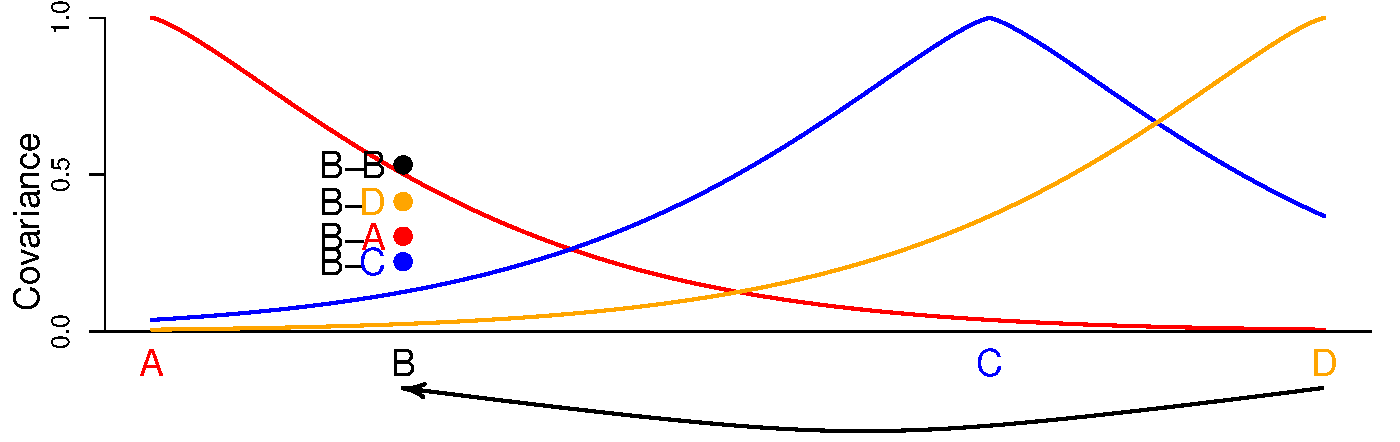
\includegraphics[width=\textwidth]{figs/sims/Admix_covar_toy_fig.pdf}
	\caption{} \label{sfig:toy_admixture}
\end{figure}

Due to its admixture from D, B has lower covariance with A than expected given its distance, somewhat higher covariance with C, and much higher covariance with D. In addition, the variance of B is lower than that of the other three populations, which each have variance $1$: the value of the covariance when the distance is zero. This lower variance results from the fact that the frequencies at $B$ represent a mixture of the frequency at $D$ and the frequency at $B$ before the admixture. 

Now, using this example scenario, let us return to the concern posed above: that admixture location and population location are not identifiable.  For the sake of simplicity, assume that we hold the locations of A, C, and D constant, as well as the decay of covariance with distance (as could be the case if A-D are part of a larger analysis).  The covariance relationships of $B$ to the other populations cannot be simply satisfied by moving $B$ towards D, as B would then have a covariance with C that is higher, and a covariance with A that is lower, than that we actually observe. 

Introducing admixture into the model allows it to satisfy all of these conditions: it can draw ancestry from D but keep part of its resemblance to A, it avoids B having to move closer to C, and it explains B's low variance.  Even in the absence of a sample from population C, B is better described as a linear mixture of a population close to A and D.  However, there are specific scenarios in which a limited sampling scheme (both in size and location), can lead to tradeoffs in the likelihood between estimated population location and that of its source of admixture.

The analyses depicted in Figures \ref{sfig:corner_admix_scenarios}\subref{corner_admix_inference}, 
\ref{barr_inland_ad}\subref{barr_inland_ad_inference}, and
\ref{barr_inland_ad}\subref{big_barr_ad_scenario}, 
give examples of these tradeoffs.
In each, the inferred admixture proportions in the admixed populations are less than those used to simulate the data,
and the admixed populations are able to explain the high covariance they have with their sources of admixture via their inferred location,
rather than just via their inferred source of admixture and admixture proportion.  
The reason they choose to do explain their anomalous covariance with their inferred location,
rather than with their admixture source,
is that we place a very harsh prior against admixture inference Table \ref{tab:param_prior_tab}.
The prior is designed to make inference conservative with respect to admixture,
but it has the side effect of skewing the posterior probability toward lower admixture proportions.


\subsection*{Empirical Applications}
Below, we describe the specifics of our analyses of the greenish warbler dataset and the global human dataset.  The analysis procedure for each dataset is given here:

For each analysis,
\begin{itemize}
\item[1.] Five independent chains were run for $5\times 10^6$ MCMC iterations each in which populations were allowed to choose their own locations (but no admixture).  Population locations were initiated at the origin (i.e.\ - at iteration 1 of the MCMC, $G_i = (0,0)$), and all other parameters were drawn randomly from their priors at the start of each chain.  
%
\item[2.]The chain with the highest posterior probability at the end of the analysis was selected and identified as the``Best Short Run".
%
\item[3.] A chain was initiated from the parameter values in the last iteration of the Best Short Run.  Because inference of admixture proportion and location was not allowed in the five initial runs, admixture proportions were initiated at 0 and admixture locations, \admixsource{G} were initiated at the origin.  This  chain (the ``Long Run") was run for $10^8$ iterations, and sampled every $10^5$ iterations for a total of $1000$ draws from the posterior.
\end{itemize}

For each dataset, we ran two analyses using the observed population locations as the prior on $G$.  
Then, to assess the potential influence of the spatial prior on population locations, 
we ran one analysis in which random, uniformly distributed locations between, 
for longitude, the minimum and maximum observed longitude, 
and, for latitude, the minimum and maximum observed latitude were used as the prior on population locations.  
For the warbler dataset, we repeated this analysis procedure, treating each sequenced individual as its own population.  
For clarity and ease of interpretation, we present a full Procrustes superimposition of the inferred population locations ($G$) 
and their sources of admixture ($\identifyadmixsource{G}$), 
using the observed latitude and longitude of the populations/individuals ($G$) to give a reference position and orientation.  
As results were generally consistent across multiple runs for each dataset regardless of the prior employed, 
we (unless stated otherwise) present only the results from the `random' prior analyses.

Finally, we compared the SpaceMix map to a map derived from a Principal Components Analysis (Patterson and Reich 2006).  For this analysis, we calculated the eigendecomposition of the mean-centered allelic covariance matrix, then plotted individuals' coordinates on the first two eigenvectors (e.g.\ Novembre et al 2008).  For consistency of presentation, we show the full Procrustes superimposition of the PC coordinate space around the geographic sampling locations.


\newpage

\bibliography{spacemix.refs}

\newpage

\appendix

\section*{Supplementary Materials}

\begin{figure}
	\centering
		{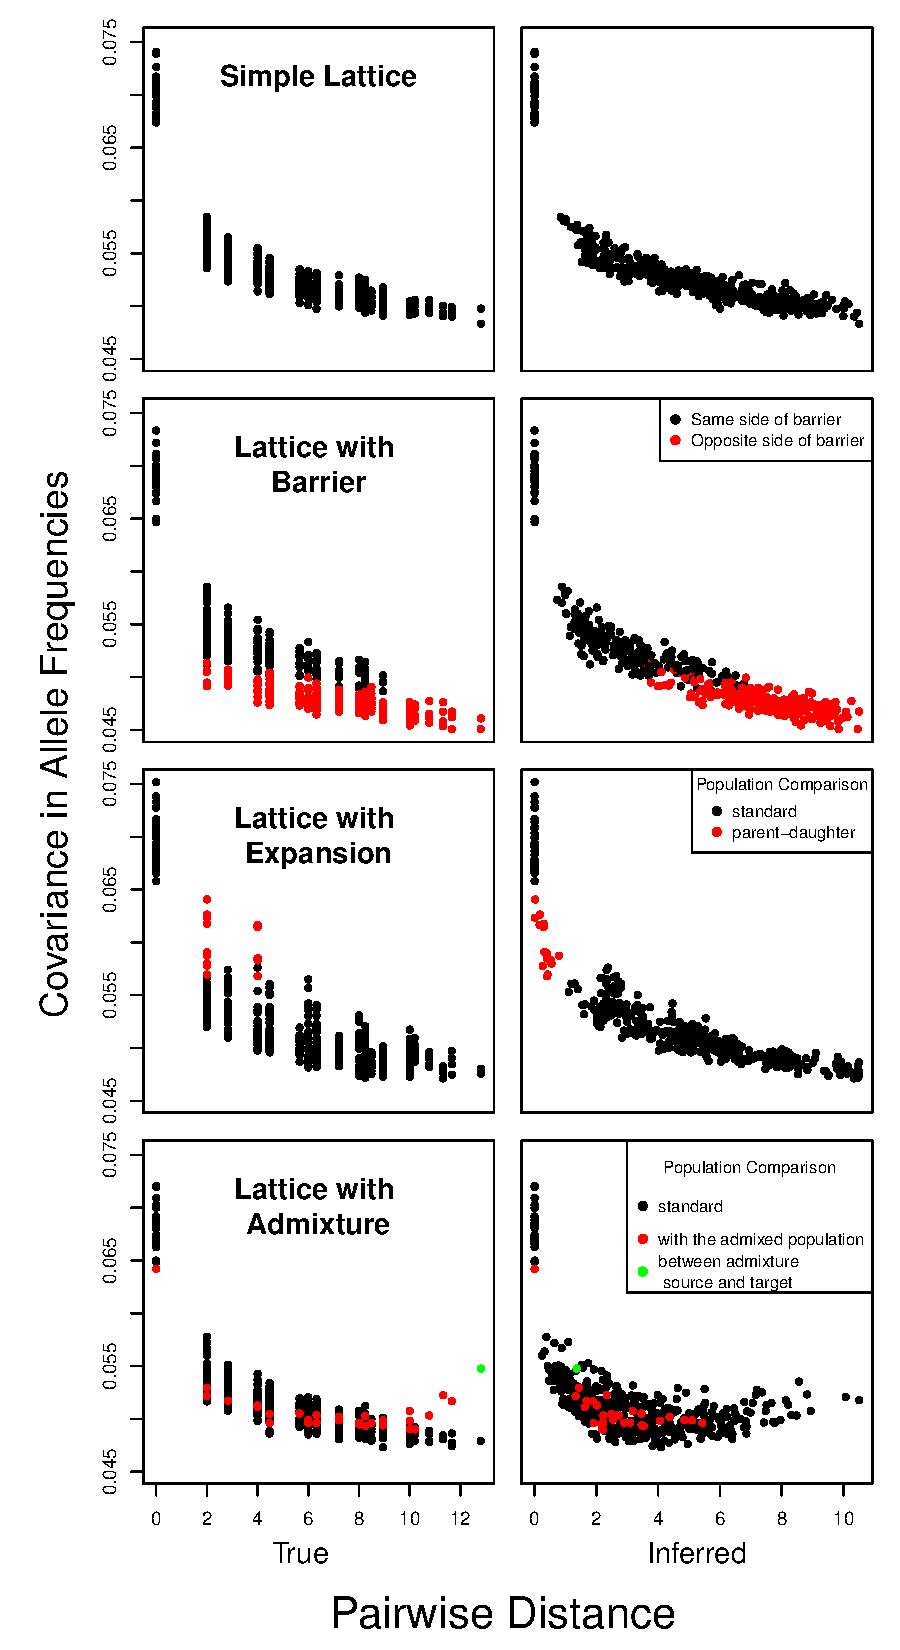
\includegraphics[width=4.8in,height=8.8in]{figs/sims/sim_covariance_decays.pdf}}
		\caption{Decays in covariance for four different simulation scenarios (from top to bottom: simple lattice; lattice with barrier; lattice with expansion; lattice with admixture).  Left column: sample covariance plotted against observed pairwise distance.  Right column: sample covariance plotted against inferred geogenetic distance.}
	\label{sfig:sim_covariance_decays}
\end{figure}


\begin{figure}
\centering
	{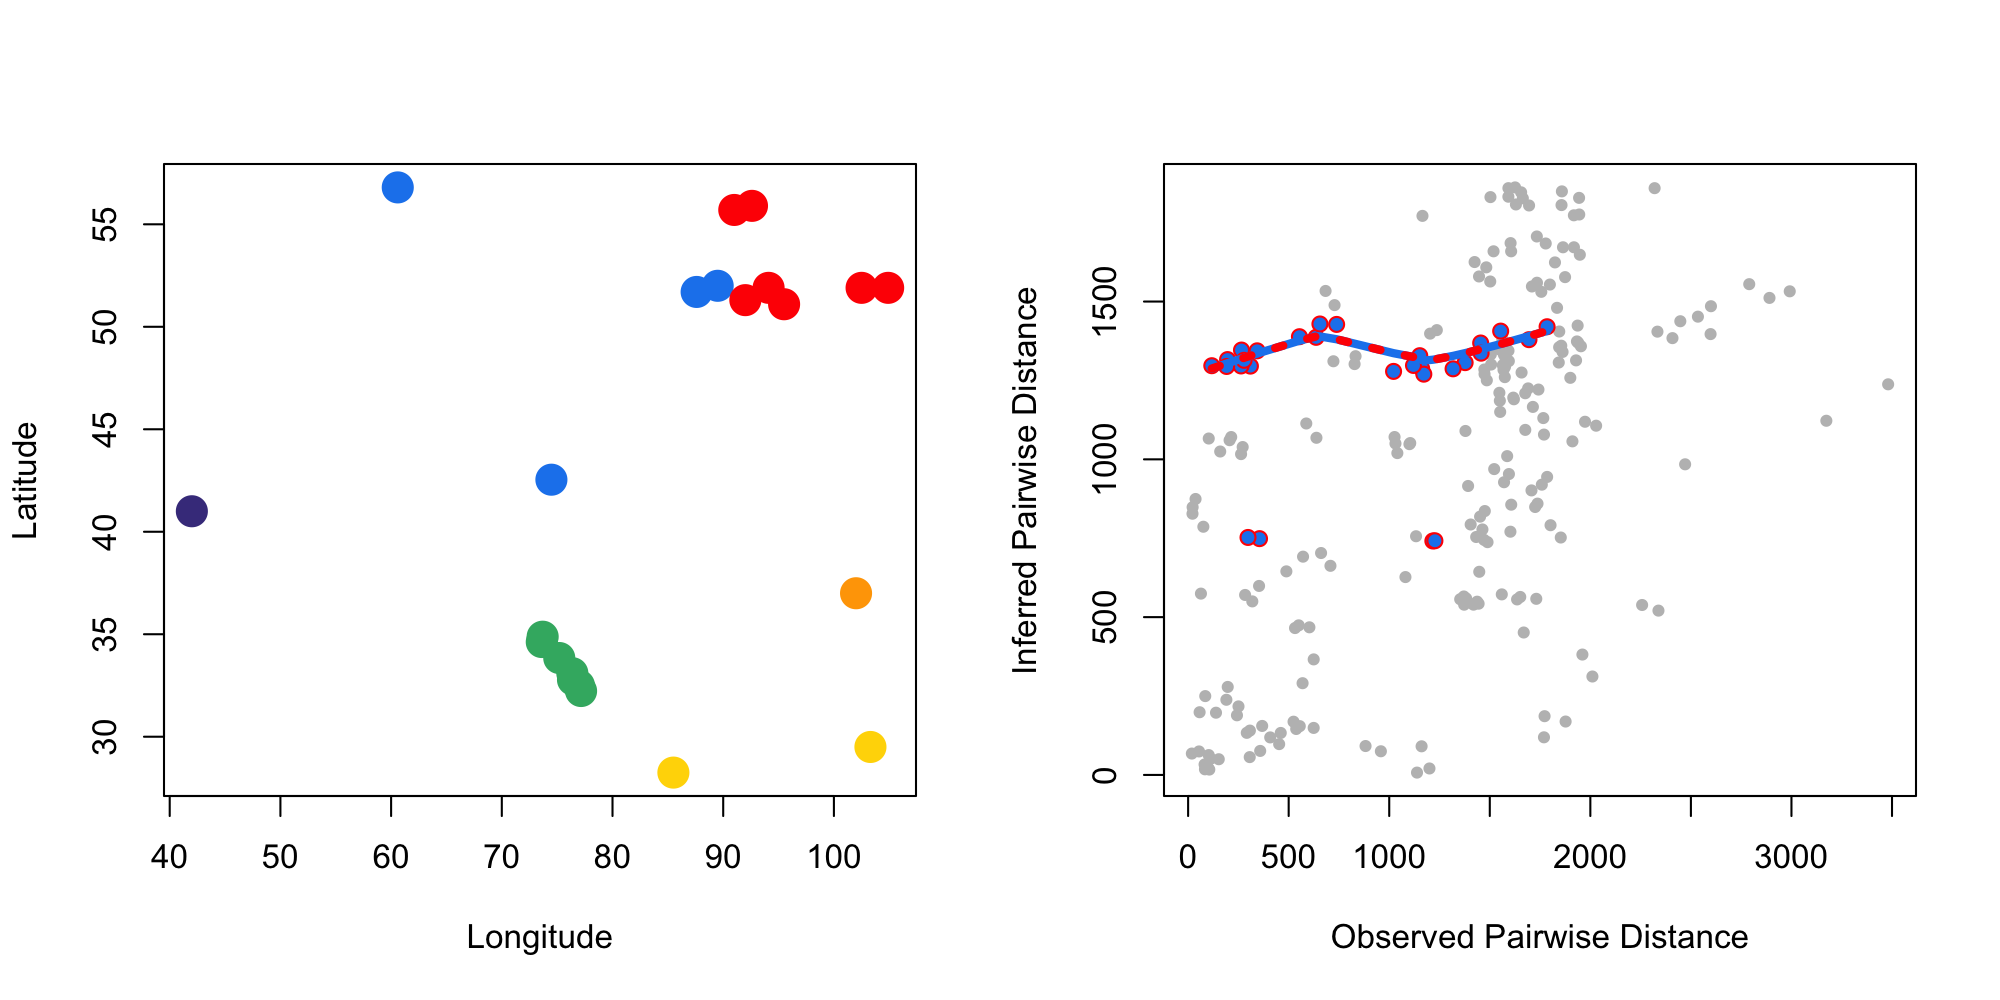
\includegraphics[width=6in,height=2.5in]{figs/warblers/warb_pop_dist_compare.png}}
	\caption{
    Comparing observed to estimated pairwise distance between warbler populations: a) observed population coordinates; b) pairwise geographic (great-circle) distance between populations compared to that between their inferred locations.  The highlighted points show distances between populations from the \textit{plumbeitarsus} and \textit{viridanus} subspecies.  Notice that, regardless of their observed distance, their inferred separations are roughly constant, and much larger than their observed distance.
    \plr{maybe instead of ``observed'' and ``inferred'', should be ``geographic'' and ``geogenetic''?}
    }
	\label{sfig:warb_pop_distcomp}
\end{figure}

\begin{figure}
	\centering
	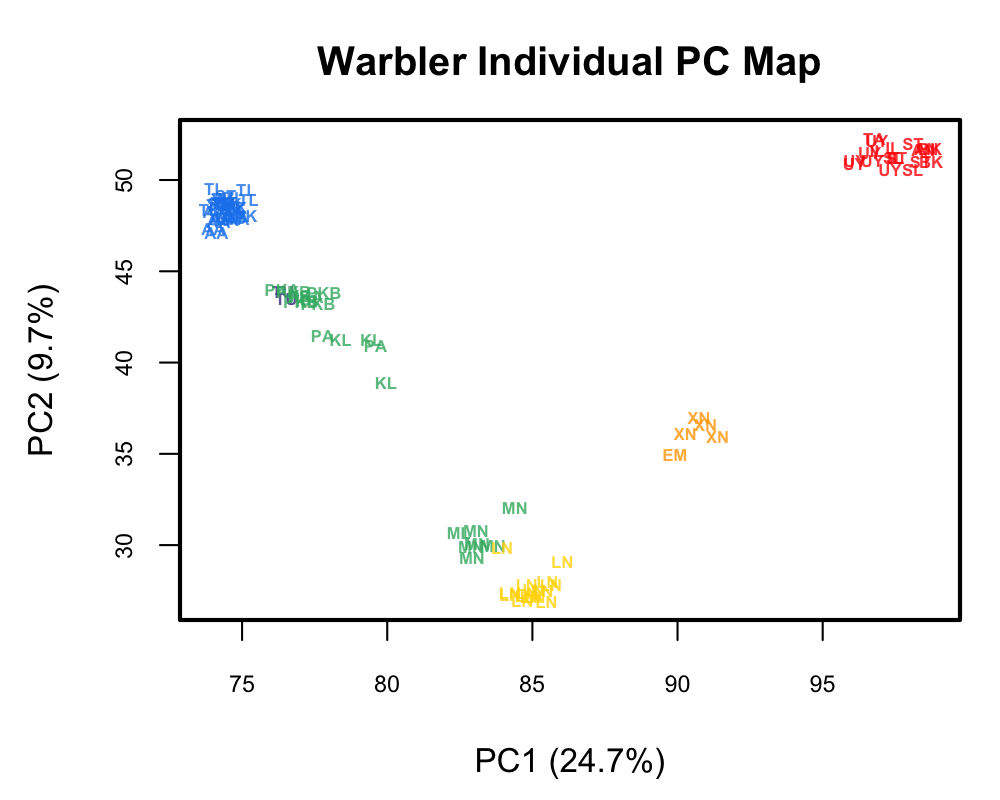
\includegraphics[width=2.4in,height=2in]{figs/warblers/warb_ind_PC_map.png}
	\caption{The map of warbler individuals derived from a Principal Components analysis.}
	\label{sfig:warb_ind_PC_map}
\end{figure}

%\gc{Graham: dont feel like we need the three analyses in main text.} Across the three independent analyses (two with the observed population locations as spatial priors on the locations, $G'$, that they choose for themselves, one with random locations as spatial priors), the inferred values of admixture proportion are consistent (95\% credible intervals:  0.146-0.233, 0.154-0.242, 0.146-0.238).  However, both the position that the Stolby population chooses for itself and the region from which it draws admixture varies between runs (Figure \ref{sfig:warbler_pop_compare}).  In two of the analyses, the Stolby population moves to a position proximate to the \textit{viridanus} cluster and chooses admixture from a point beyond the \textit{plumbeitarsus} cluster, and in one analysis, this pattern is reversed.  

\begin{figure}
	\centering
		\subcaptionbox{\label{warb_pop_realpr1}}
			{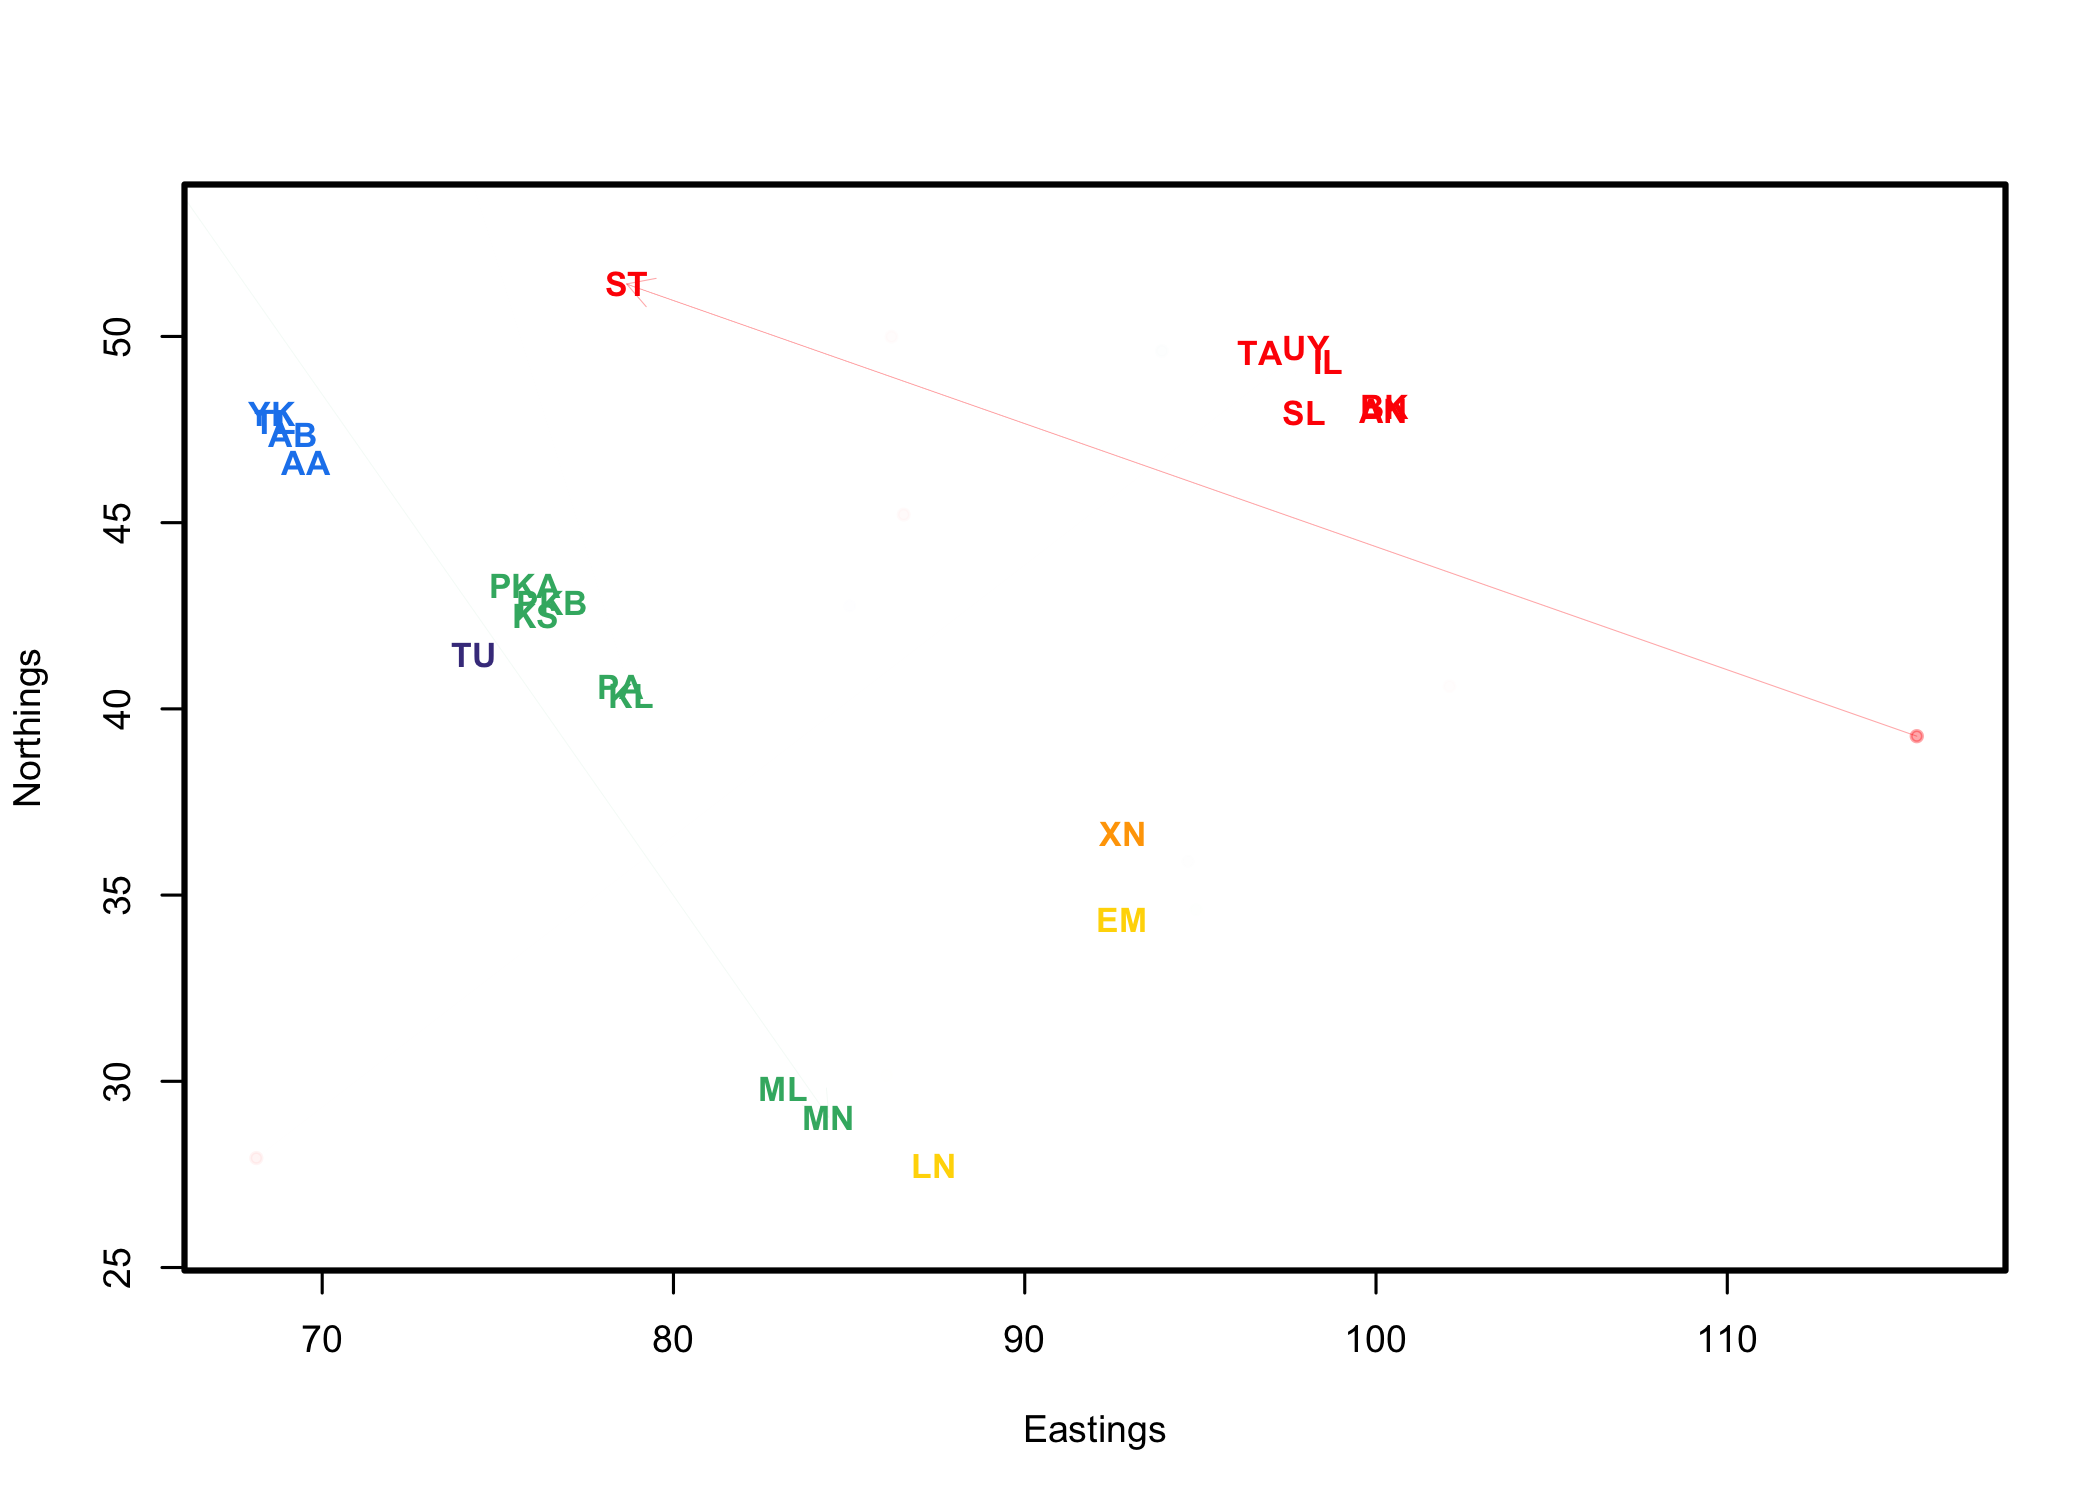
\includegraphics[width=1.85in,height=1.54in]{figs/warblers/population_warbler_map_realpr1.png}}
		\subcaptionbox{\label{warb_pop_realpr2}}			
			{\includegraphics[width=1.85in,height=1.54in]{figs/warblers/population_warbler_map_realpr2.png}}
		\subcaptionbox{\label{warb_pop_randpr1}}
			{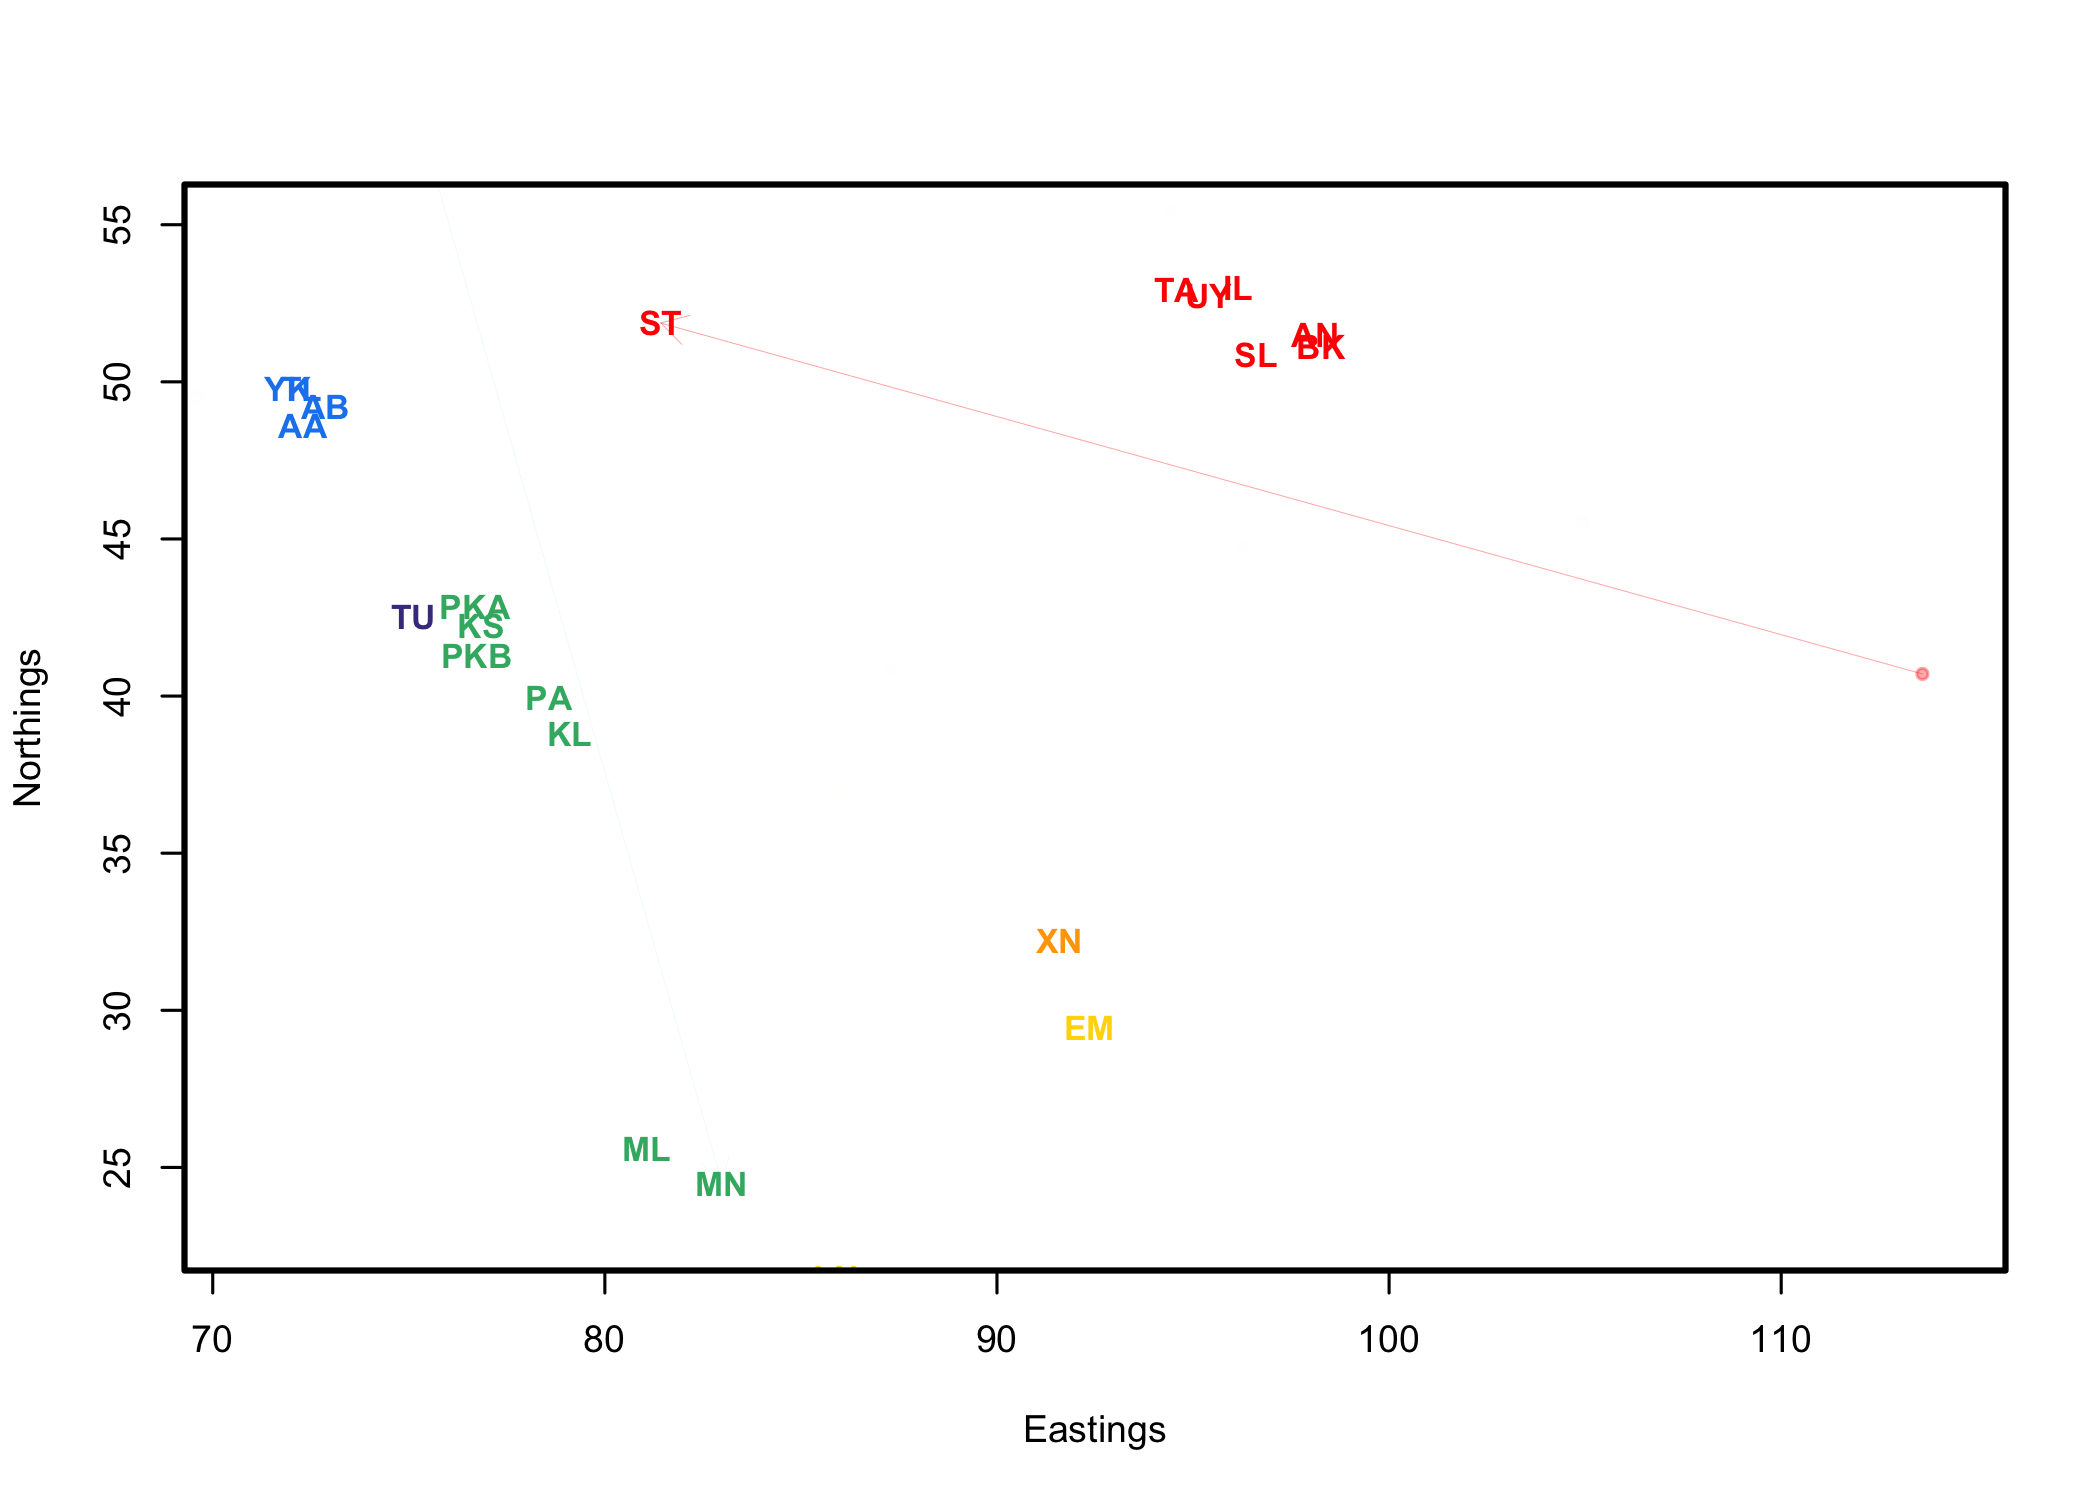
\includegraphics[width=1.85in,height=1.54in]{figs/warblers/population_warbler_map_randpr1.png}}
	\caption{Comparison of inferred maps from three independent analyses.  (a,b) Results from analysis using observed locations as priors on population locations.  (c) Results from analysis using random, uniformly distributed locations within the observed range of latitude and longitude as priors on population locations.}\label{sfig:warbler_pop_compare}
\end{figure}

\begin{figure}
	\centering
		\subcaptionbox{Likelihood \label{admix_prop_func_loc_lnl}}
			{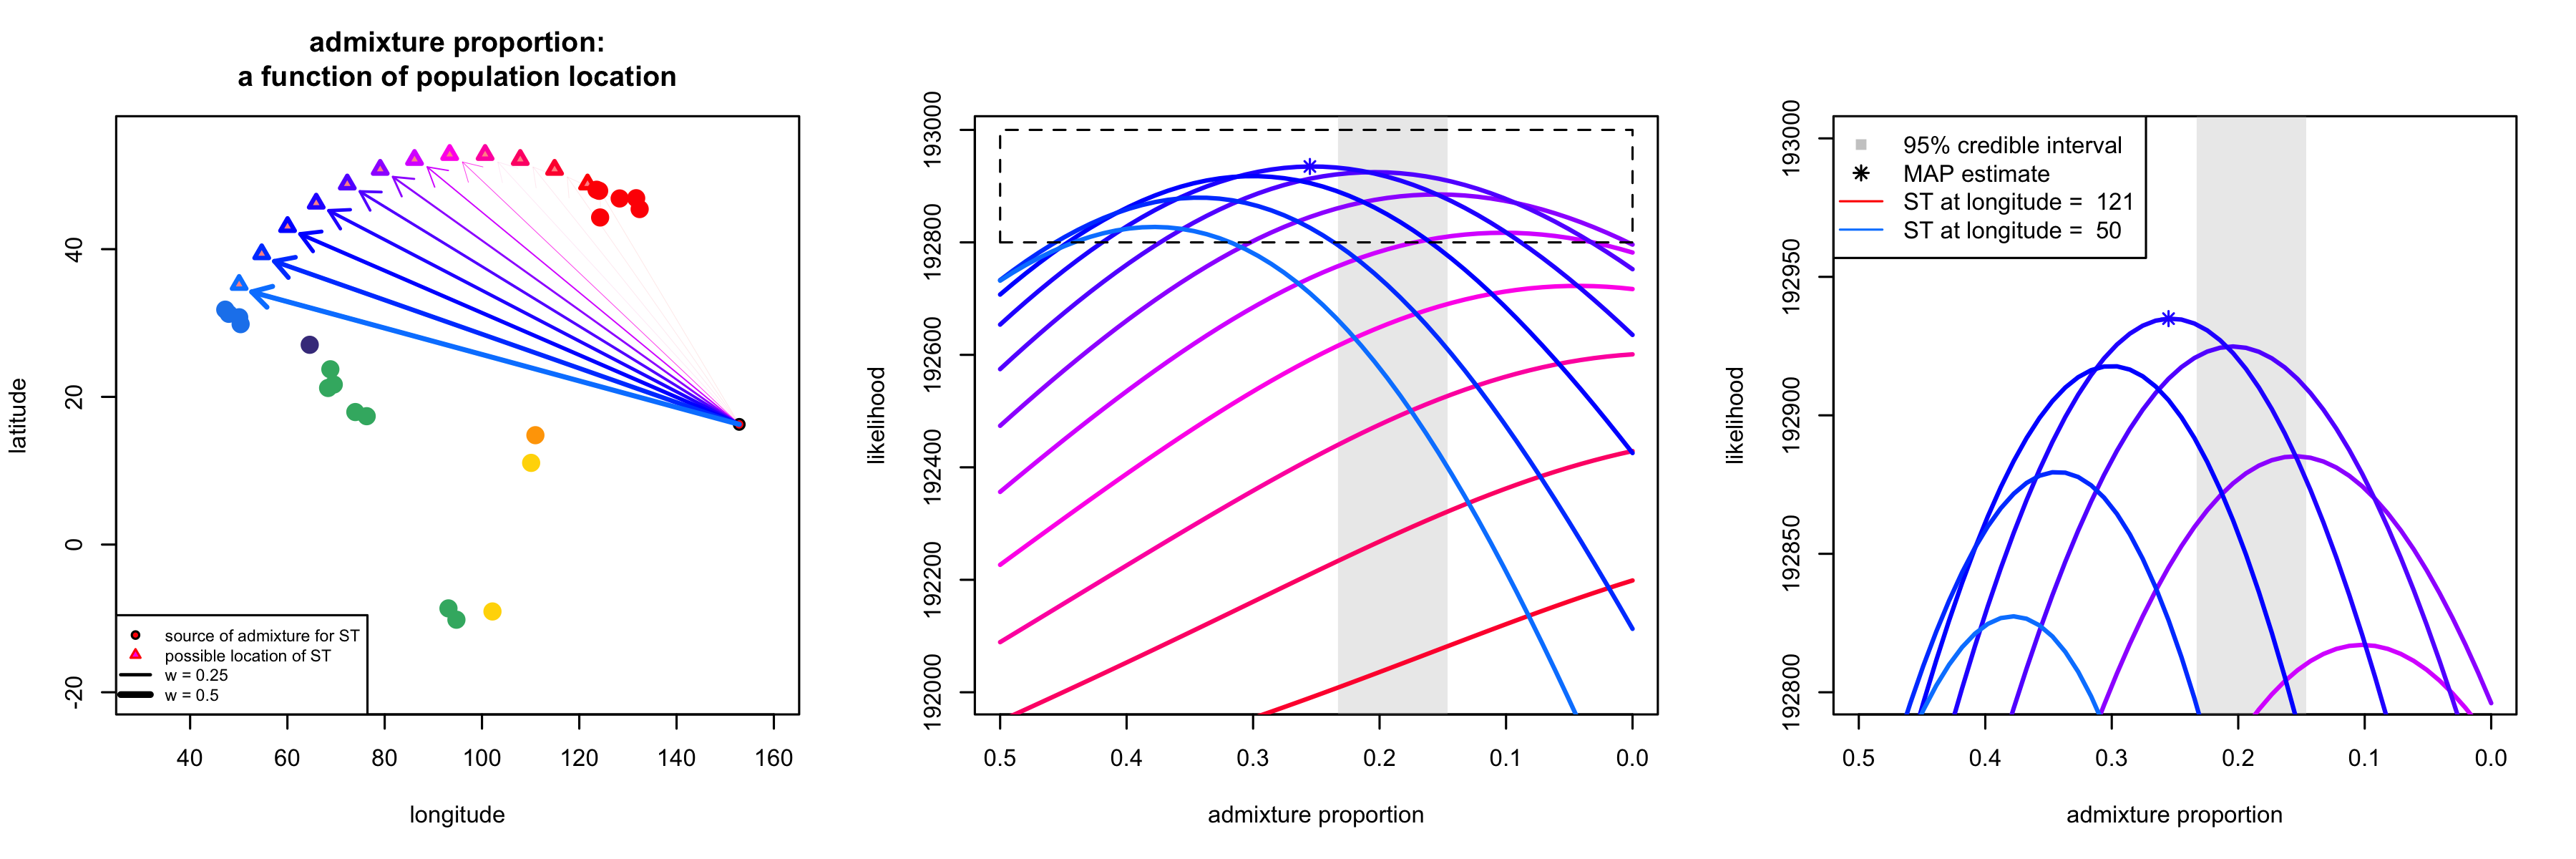
\includegraphics[width=6in,height=2in]{figs/warblers/admix_prop_func_loc_lnl.png}}
		\subcaptionbox{Posterior probability \label{admix_prop_func_loc_prob}}
			{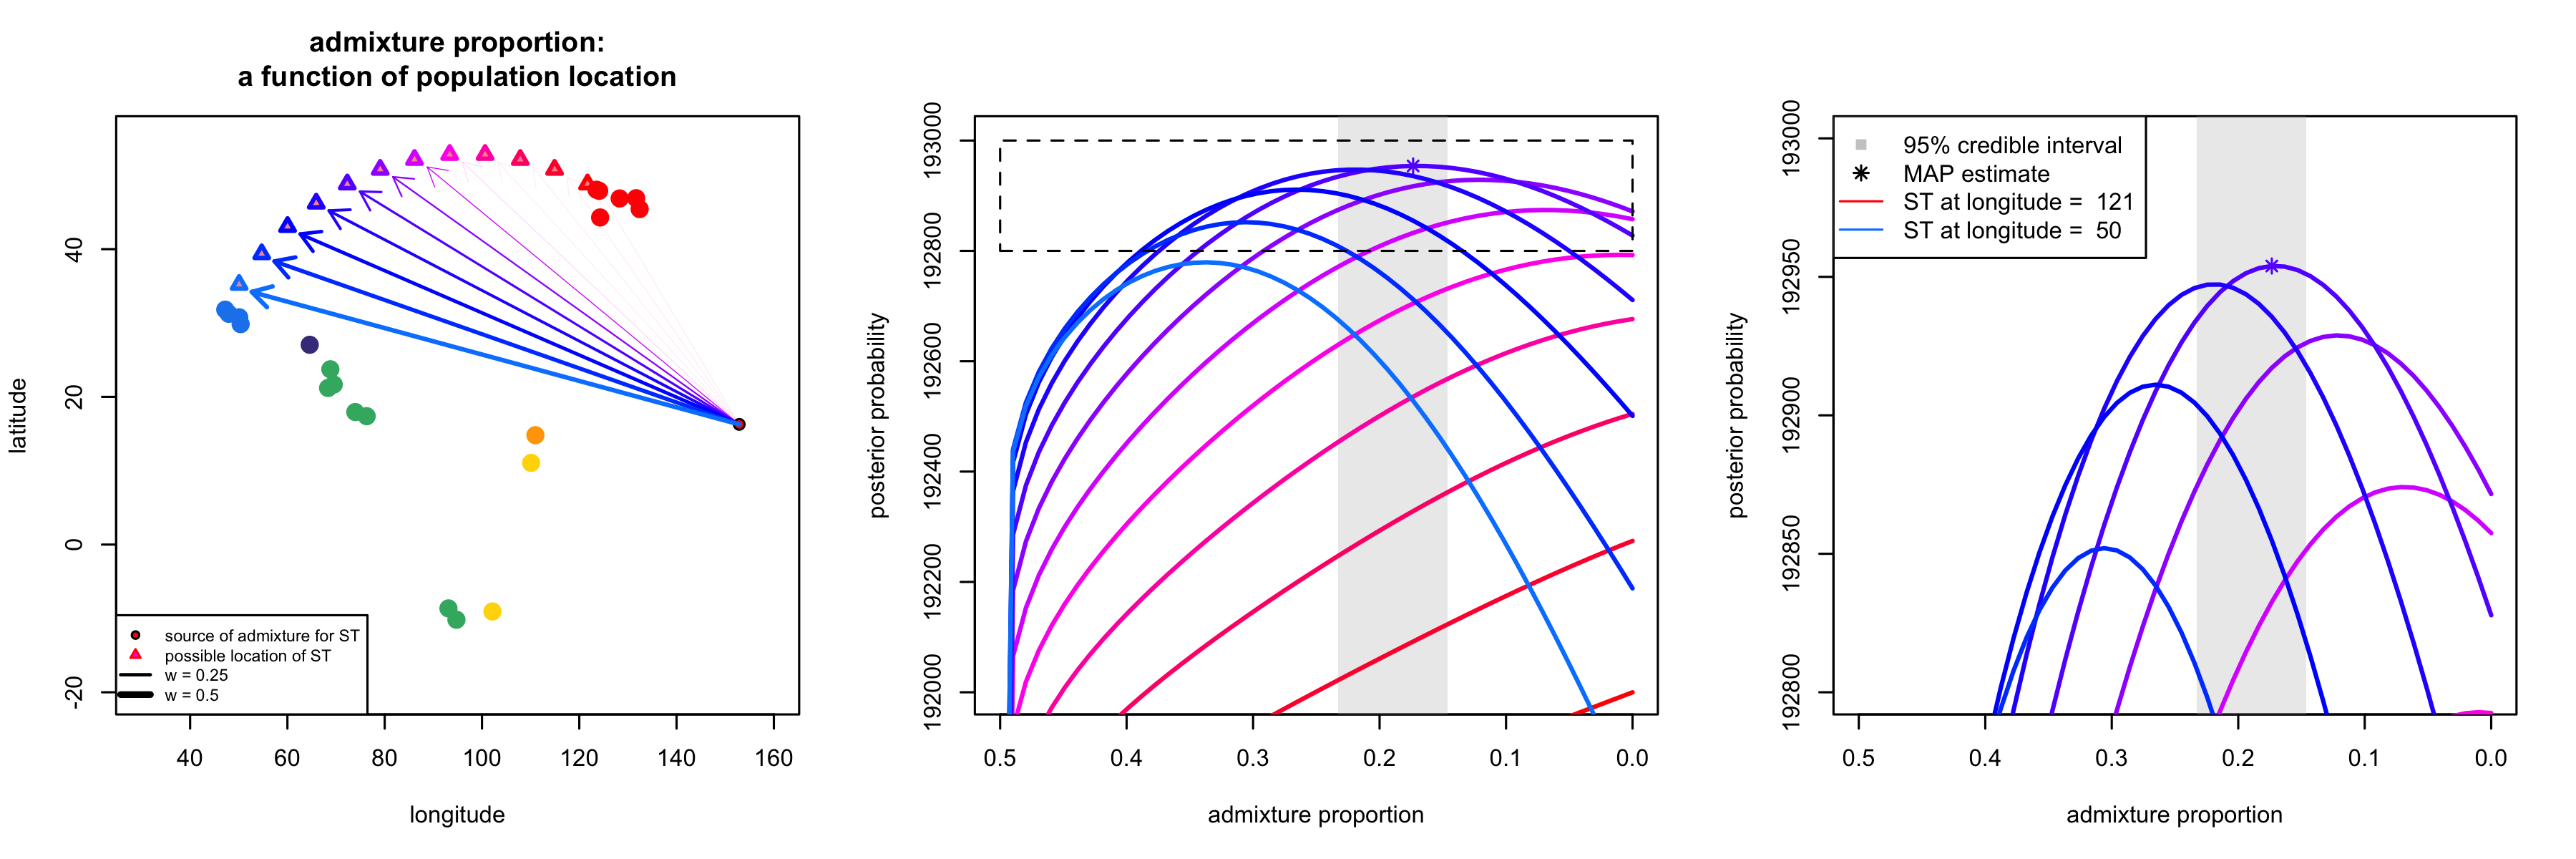
\includegraphics[width=6in,height=2in]{figs/warblers/admix_prop_func_loc_prob.png}}
	\caption{Likelihood surfaces for different placements of population ST between \textit{plumbeitarsus} and \textit{viridanus} clusters: (a) log likelihood surface; (b) posterior probability surface, incorporating the priors.}\label{sfig:admix_prop_func_loc}
\end{figure}

\begin{figure}
\centering
	{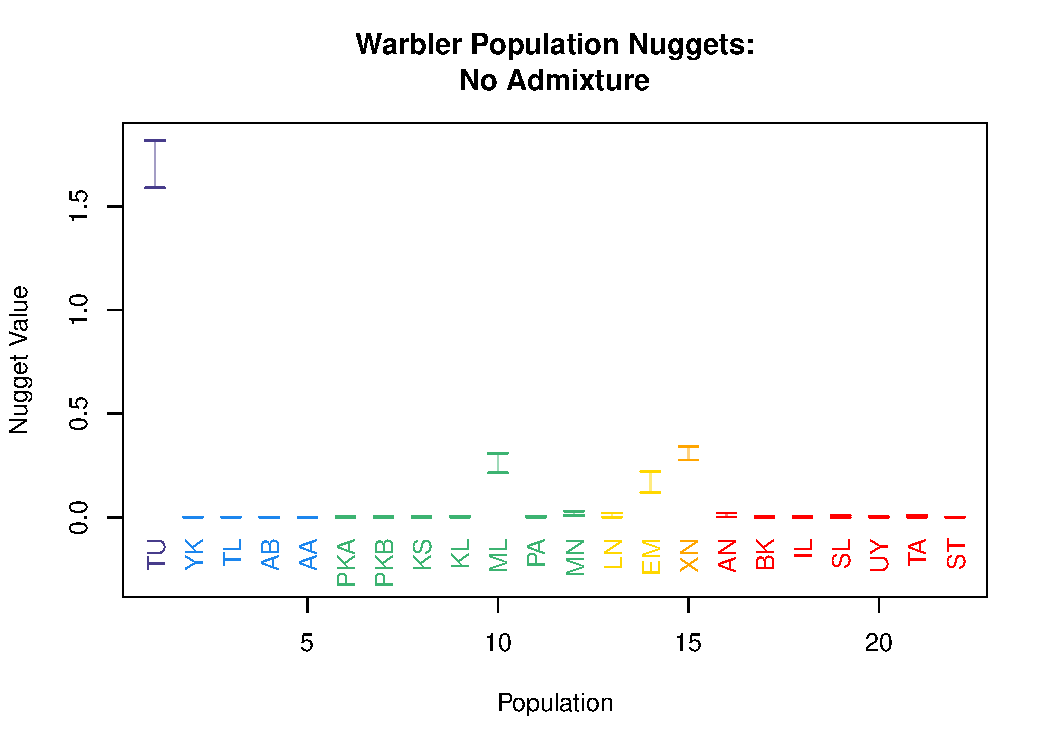
\includegraphics[width=5in,height=3.6in]{figs/warblers/warb_pop_NoAd_nugget.pdf}}
	\caption{Credible intervals on estimated warbler population nugget parameters in an analysis without admixture.}\label{sfig:warb_pop_noad_nugg}
\end{figure}

\begin{figure}
\centering
	{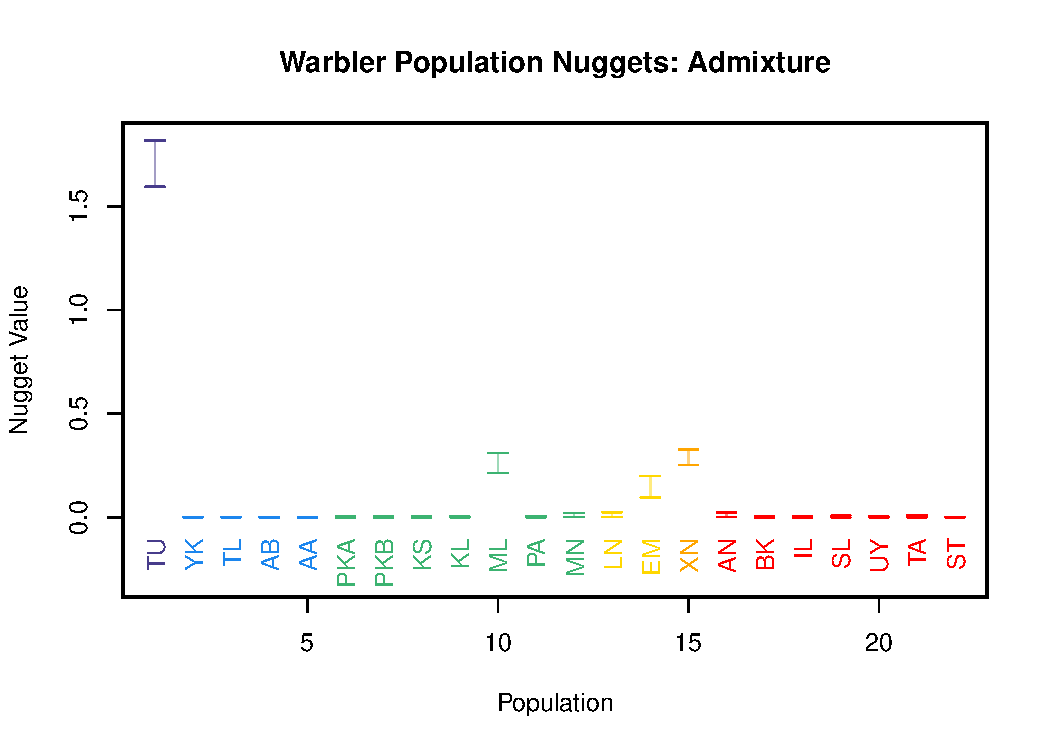
\includegraphics[width=5in,height=3.6in]{figs/warblers/warb_pop_Ad_nugget.pdf}}
	\caption{Credible intervals on estimated warbler population nugget parameters in an analysis with admixture.}\label{sfig:warb_pop_ad_nugg}
\end{figure}

\begin{figure}
\centering
	{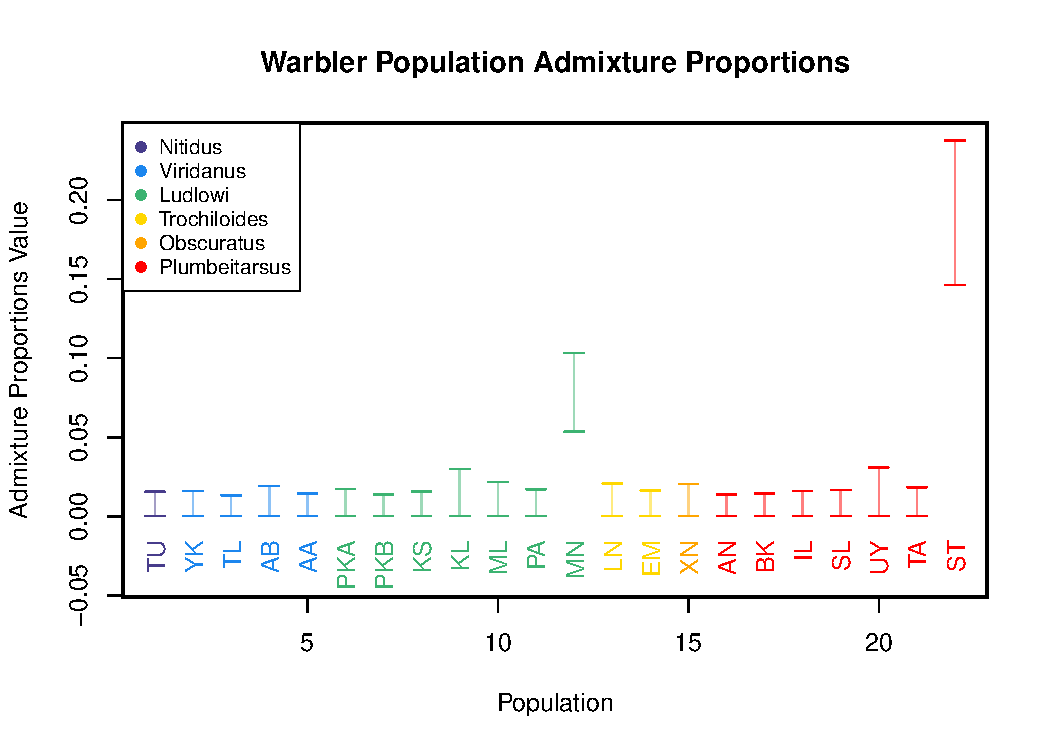
\includegraphics[width=5in,height=3.6in]{figs/warblers/warb_pop_adprop.pdf}}
	\caption{Credible intervals on estimated warbler population admixture proportion parameters.}\label{sfig:warb_pop_adprop}
\end{figure}

\begin{figure}
	\centering
		\subcaptionbox{Warbler individuals map, no admixture \label{warb_ind_noad}}
			{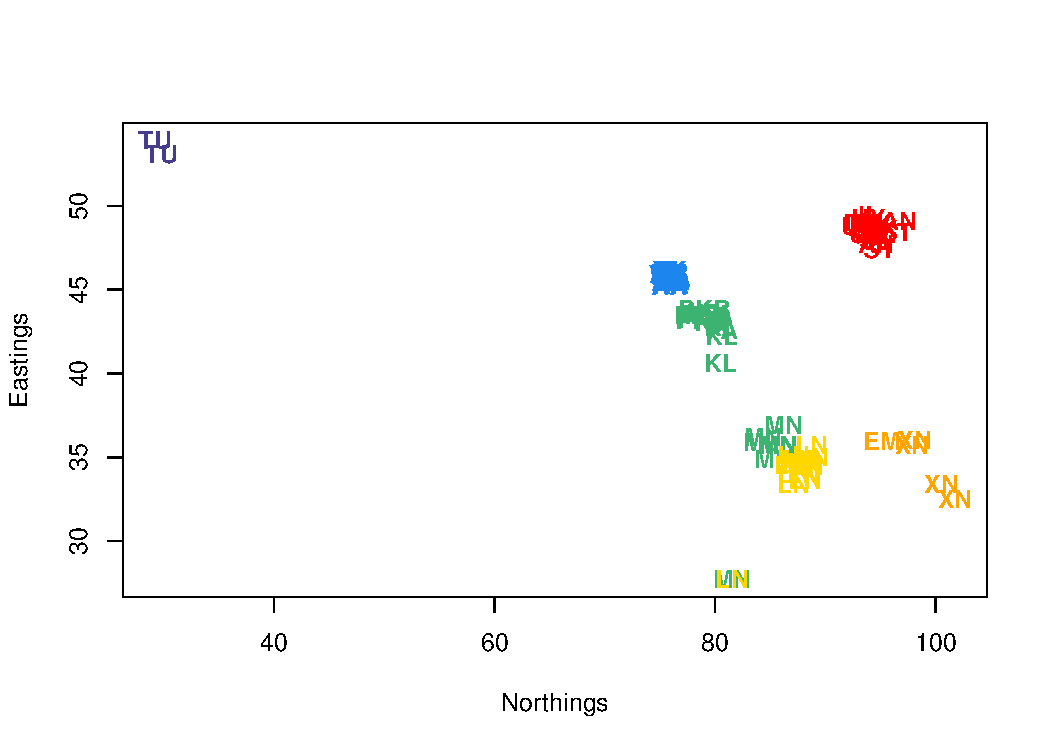
\includegraphics[width=2.8in,height=2.3in]{figs/warblers/warb_ind_noad.pdf}}
		\subcaptionbox{Closeup of non-\textit{nitidus} samples \label{warb_ind_noad_closeup}}
			{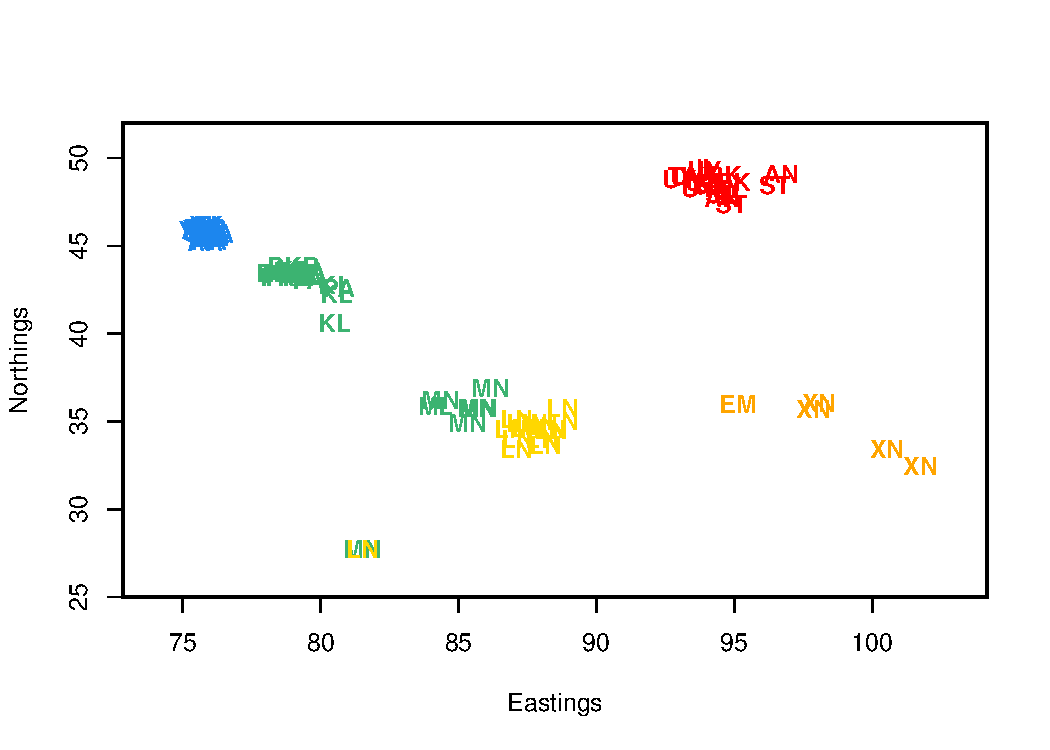
\includegraphics[width=2.8in,height=2.3in]{figs/warblers/warb_ind_noad_closeup.pdf}}
		\subcaptionbox{Warbler individuals map, admixture \label{warb_ind_ad}}
			{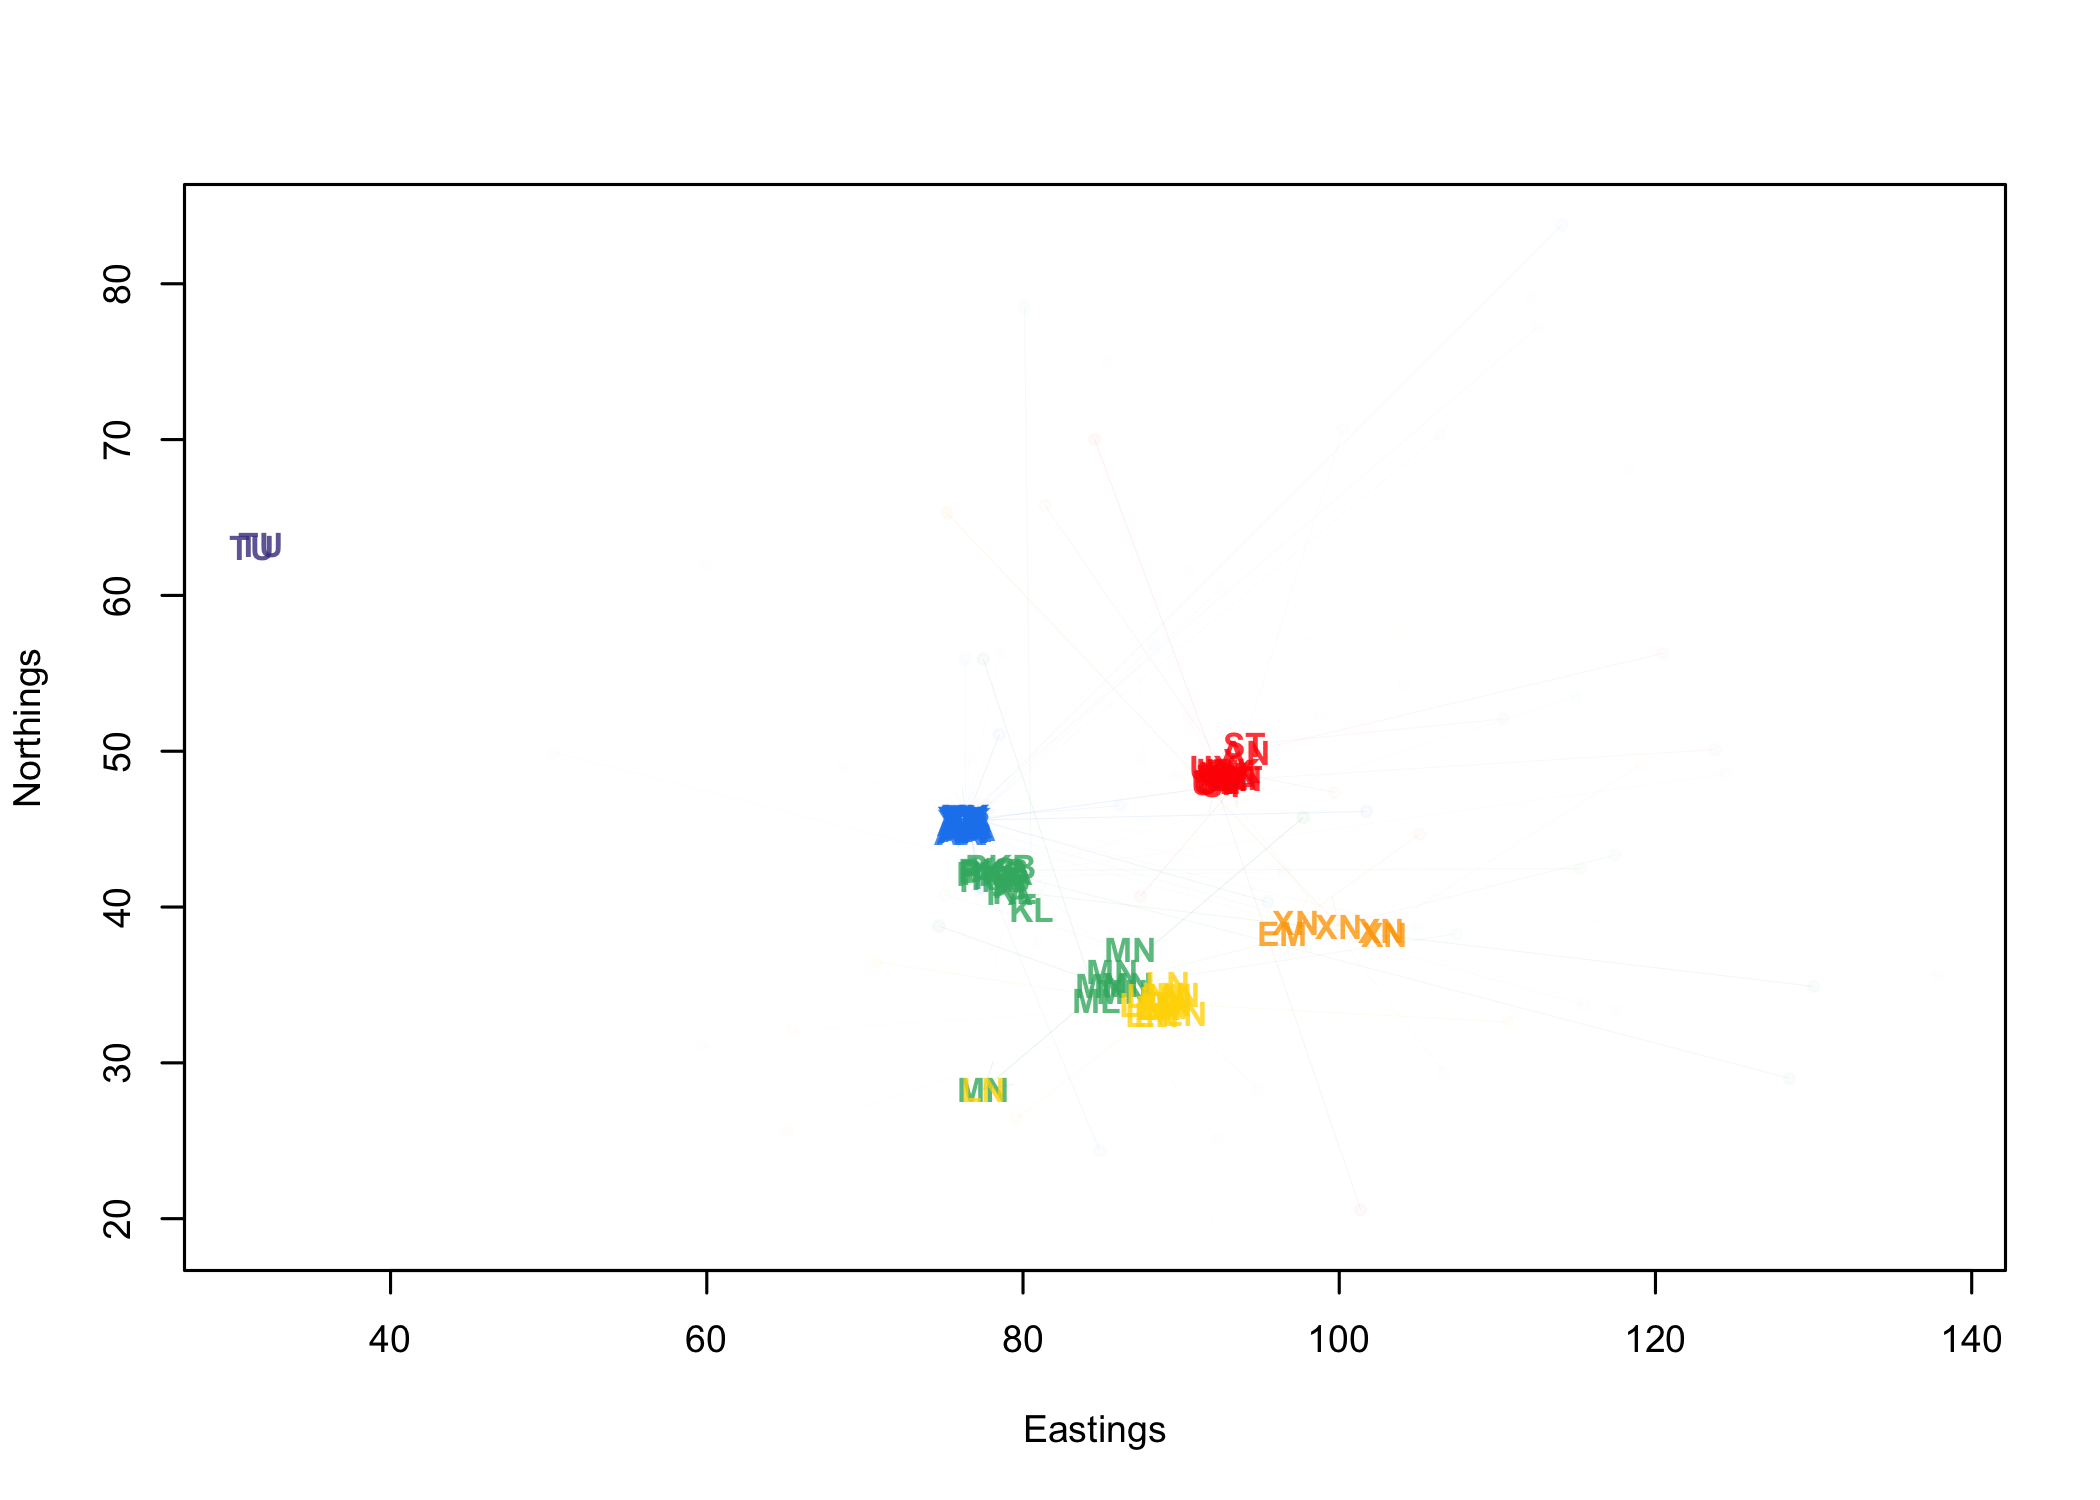
\includegraphics[width=2.8in,height=2.3in]{figs/warblers/individual_warbler_map_arrows_randpr1.png}}
		\subcaptionbox{Closeup of non-\textit{nitidus} samples \label{warb_ind_ad_closeup}}
			{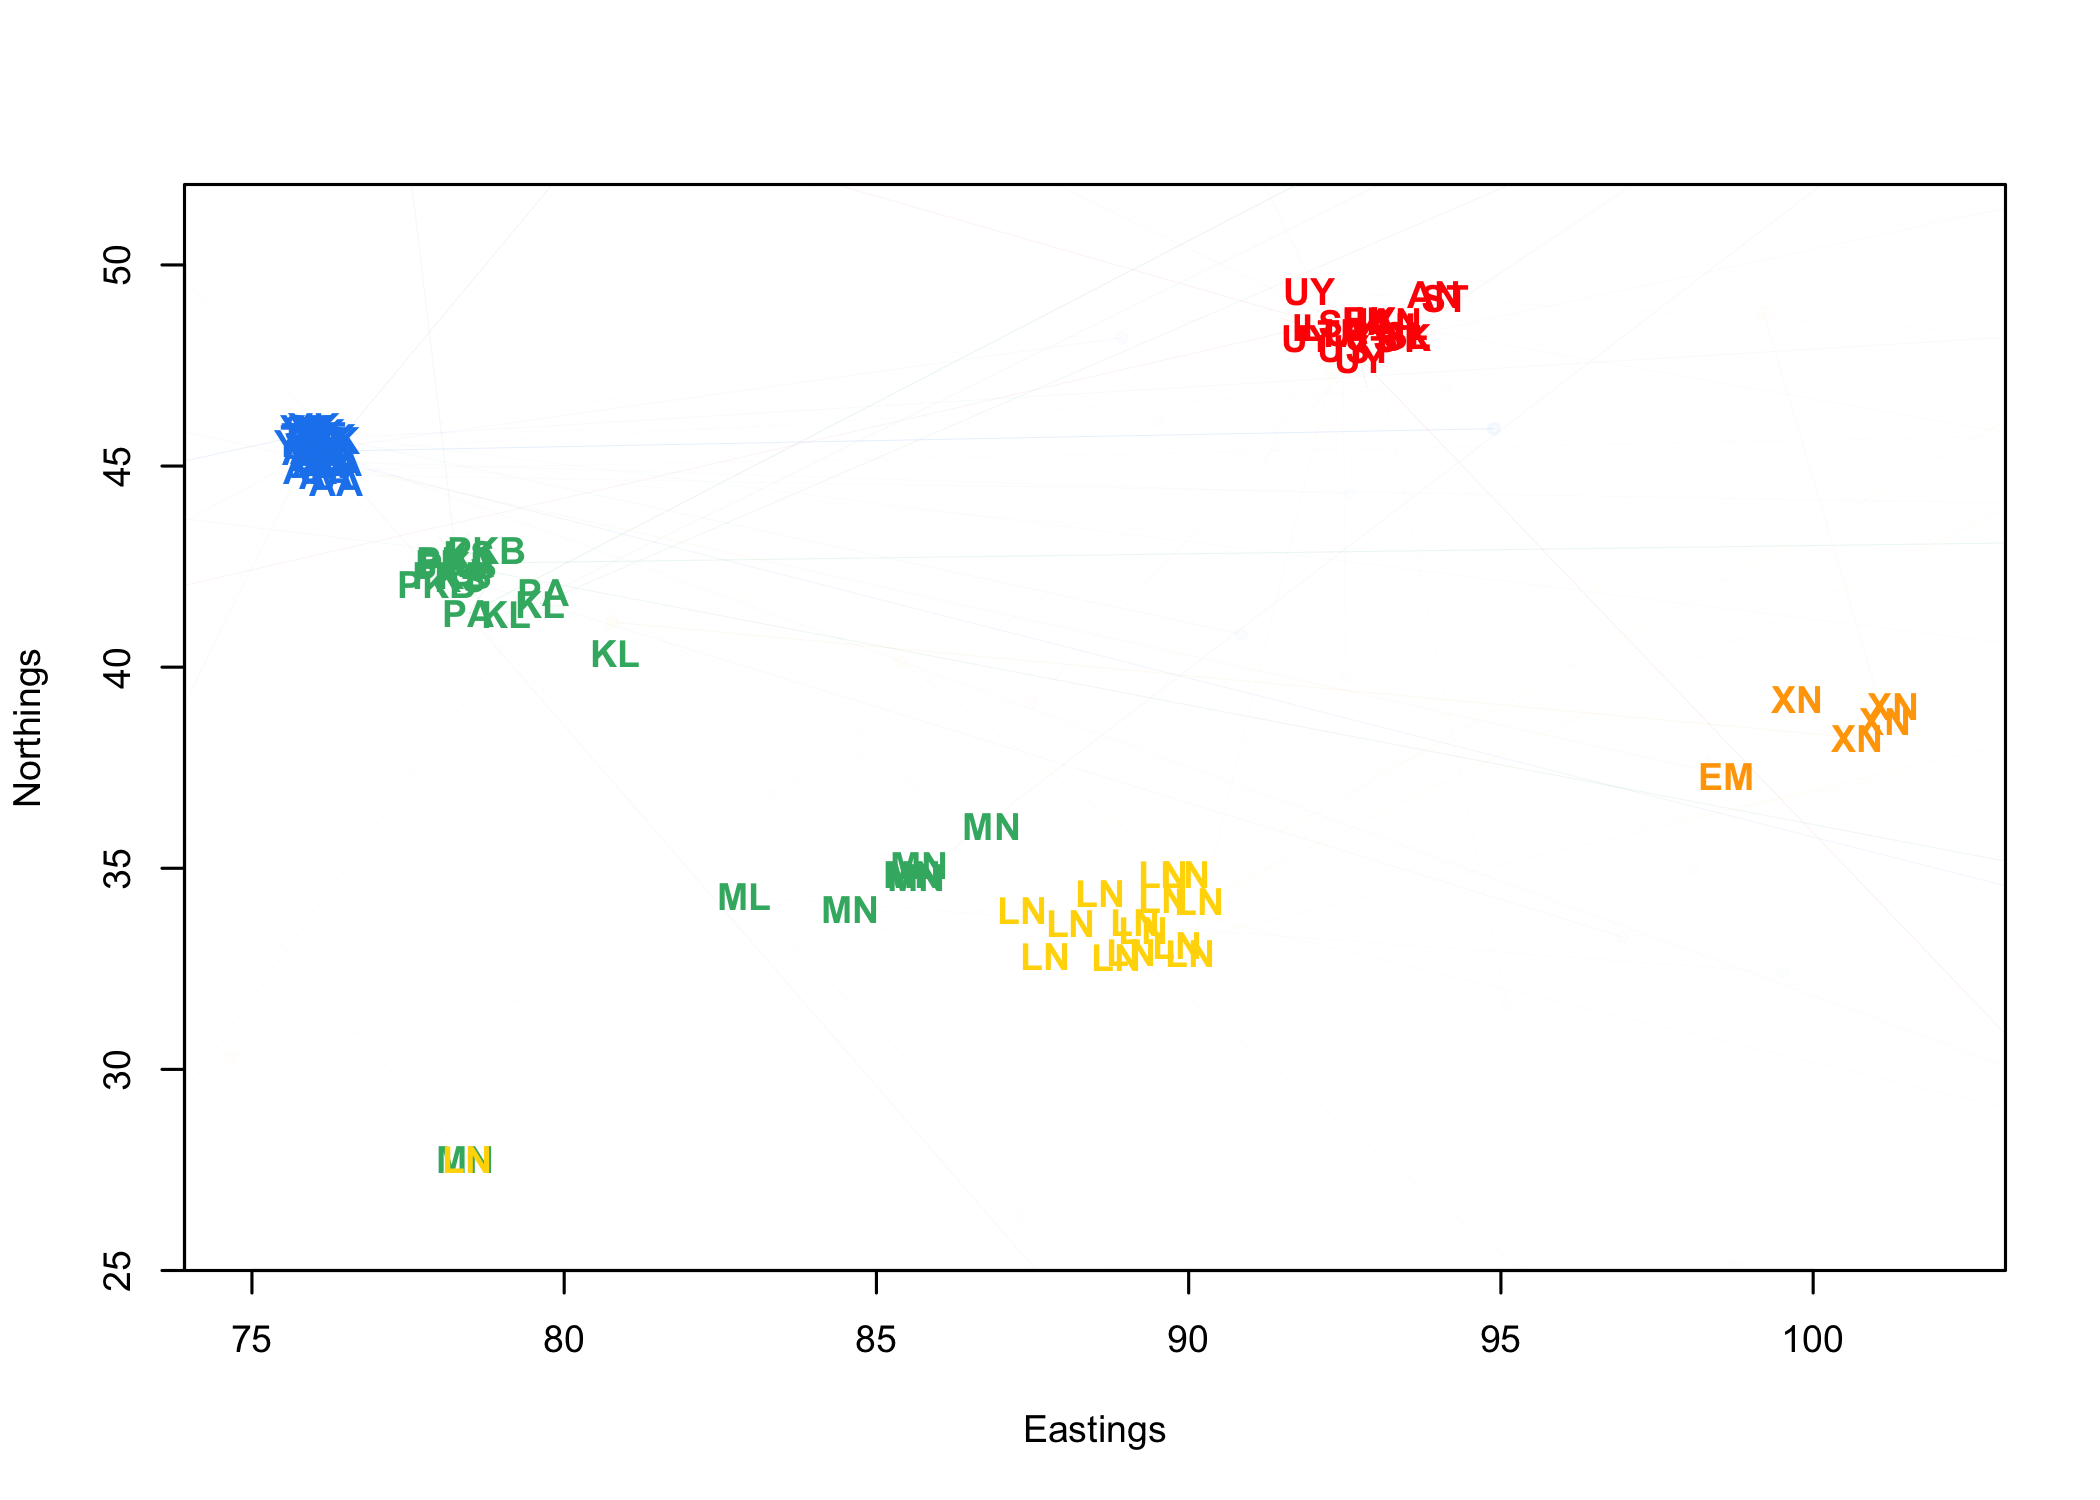
\includegraphics[width=2.8in,height=2.3in]{figs/warblers/individual_warbler_map_arrows_randpr1_closeup.png}}
	\caption{
    Inferred maps for warbler individuals, colored by subspecies under analyses with and without admixture inference. a) map inferred without admixture; (b) close up of all non-\textit{nitidus} samples in non-admixture map; c) map inferred with admixture; d) closeup of all non-\textit{nitrides} samples in the admixture map.}\label{sfig:warbler_ind_maps_compare}
\end{figure}

\begin{figure}
	\centering
		\subcaptionbox{random location prior \label{post_map_randpr2}}
			{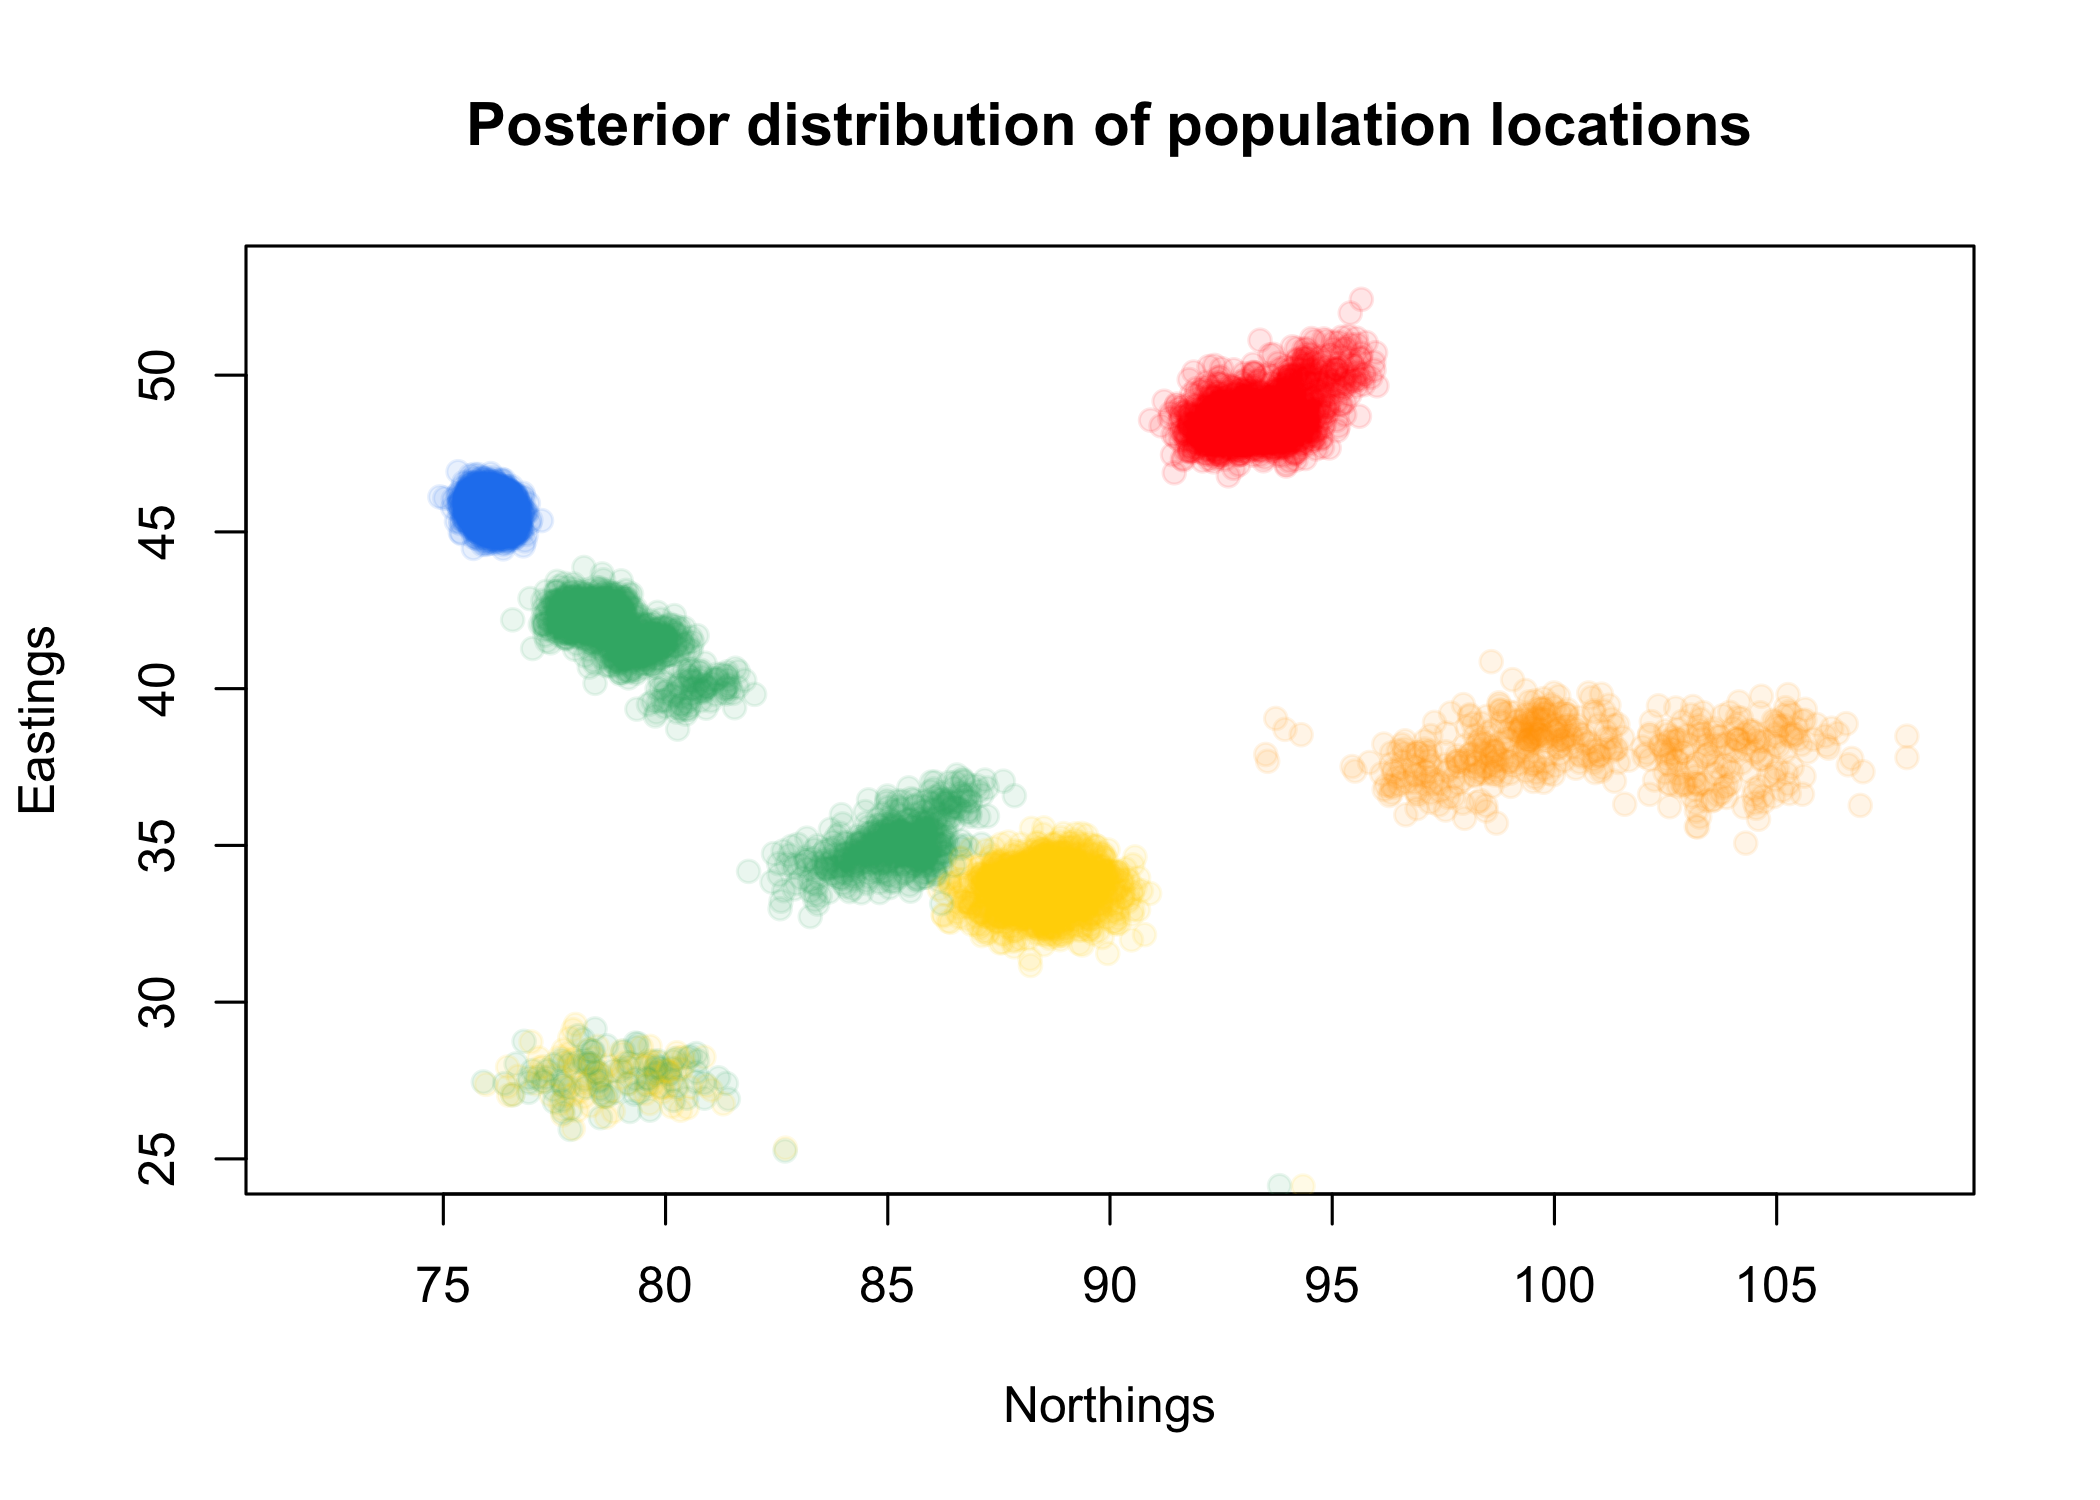
\includegraphics[width=5in,height=3.6in]{figs/warblers/warb_inds_ad_post_map_randpr2.png}}
		\subcaptionbox{random location prior \label{post_map_realpr1}}
			{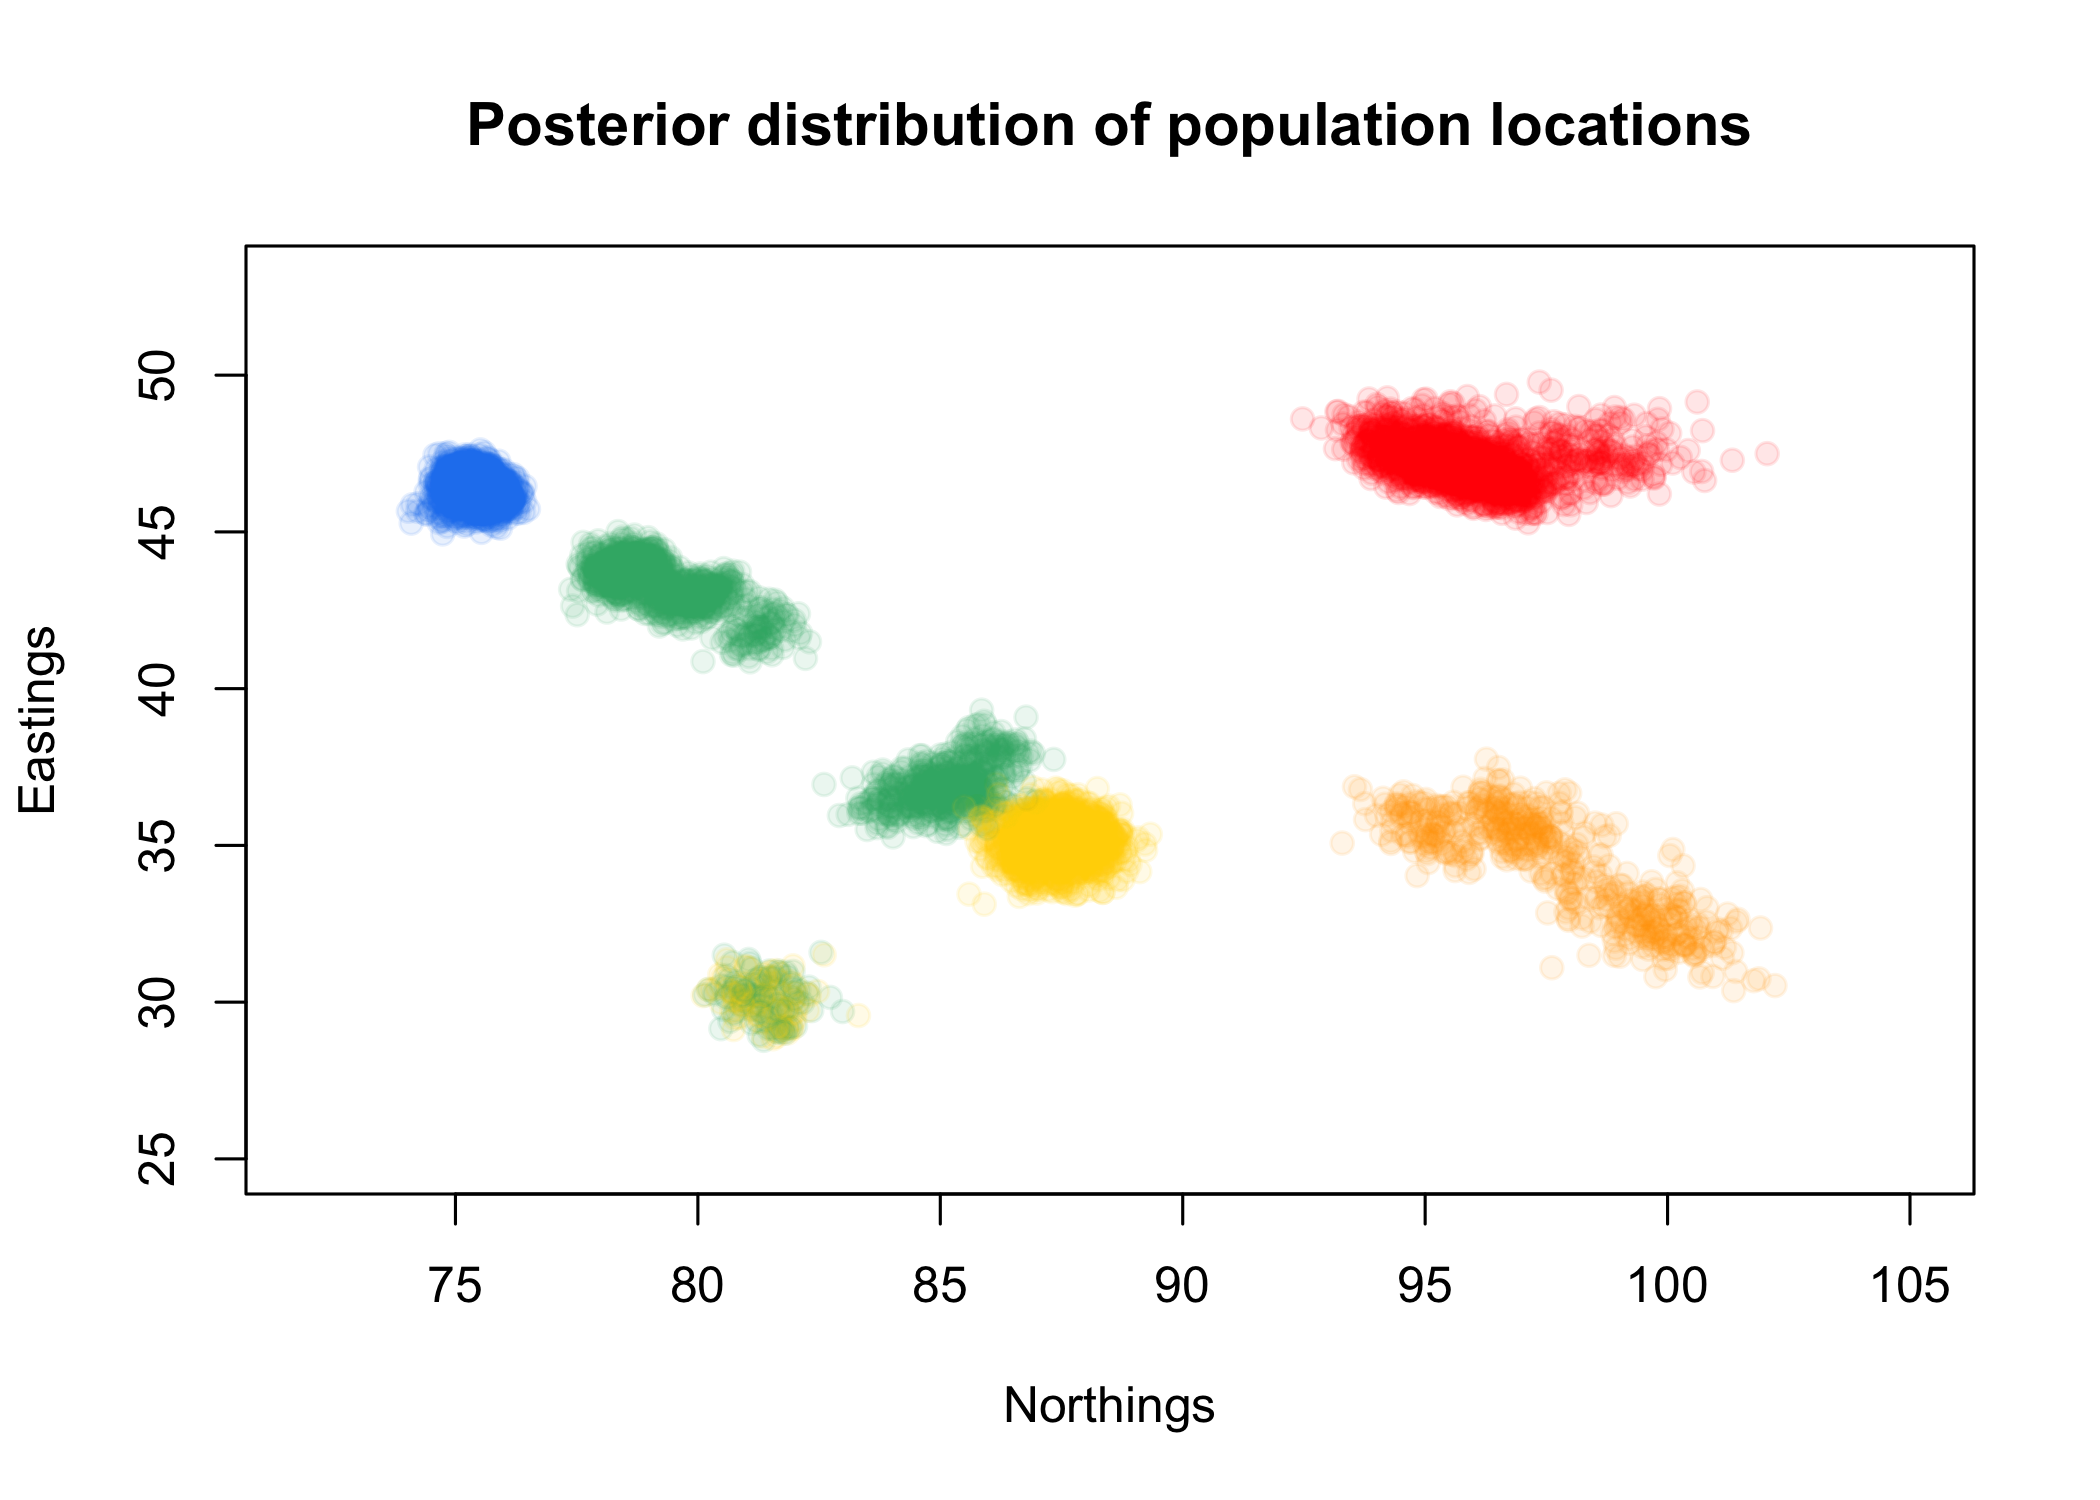
\includegraphics[width=5in,height=3.6in]{figs/warblers/warb_inds_ad_post_map_realpr1.png}}
		\subcaptionbox{random location prior \label{post_map_realpr2}}
			{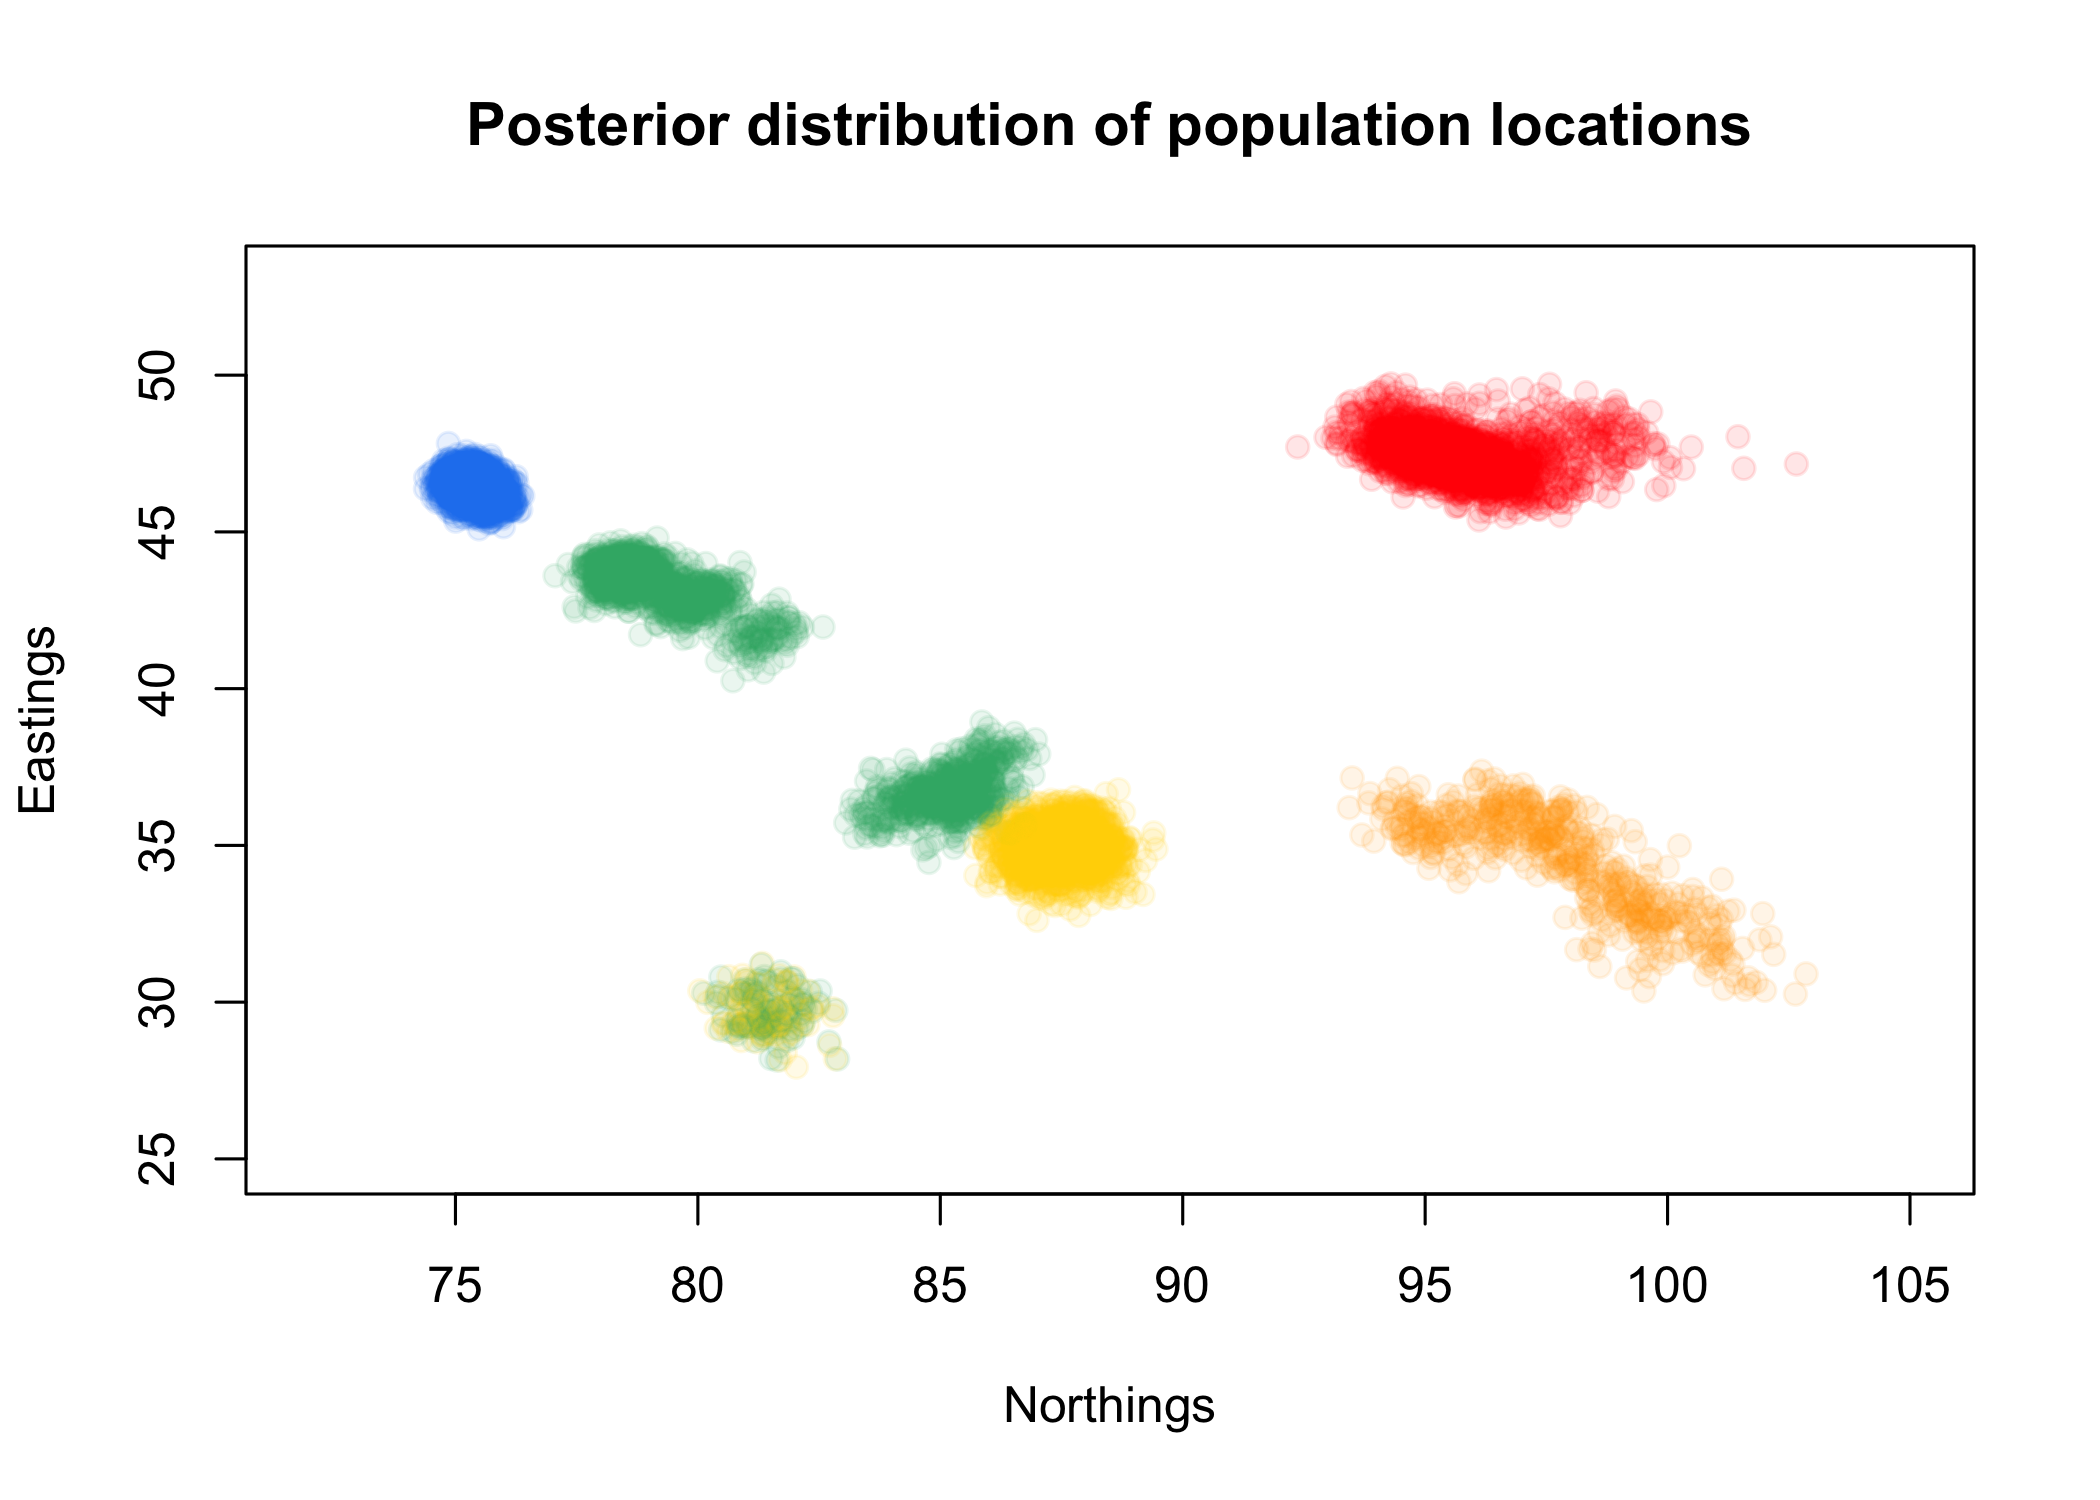
\includegraphics[width=5in,height=3.6in]{figs/warblers/warb_inds_ad_post_map_realpr2.png}}
	\caption{Maps of the posterior distributions on population locations in three separate SpaceMix analyses on the warbler individual dataset.}\label{sfig:warb_ind_clouds}
\end{figure}

\begin{figure}
\centering
	{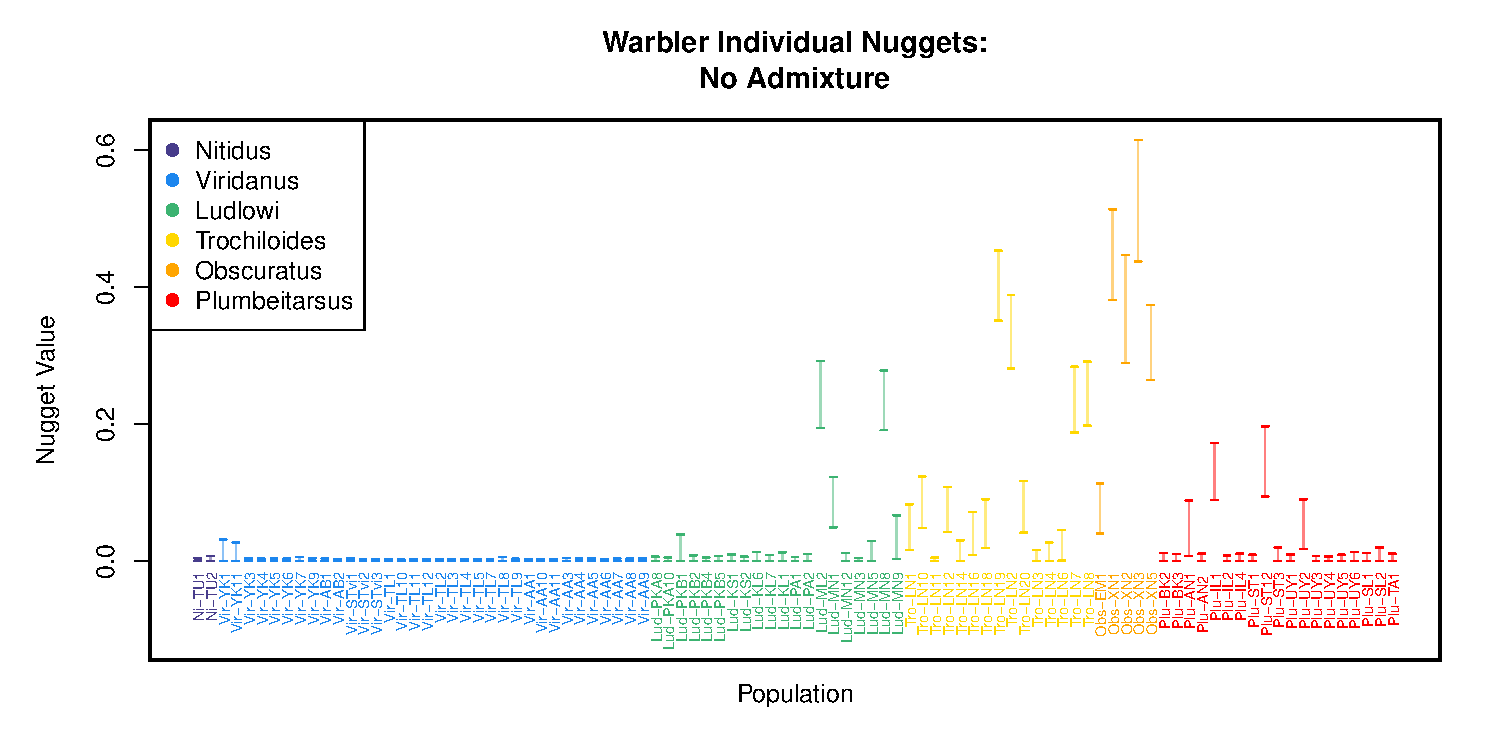
\includegraphics[width=5in,height=2.5in]{figs/warblers/warb_ind_NoAd_nugget.pdf}}
	\caption{Credible intervals on estimated warbler individual nugget parameters in an analysis without admixture.}\label{sfig:warb_ind_noad_nugg}
\end{figure}


\begin{figure}
\centering
	{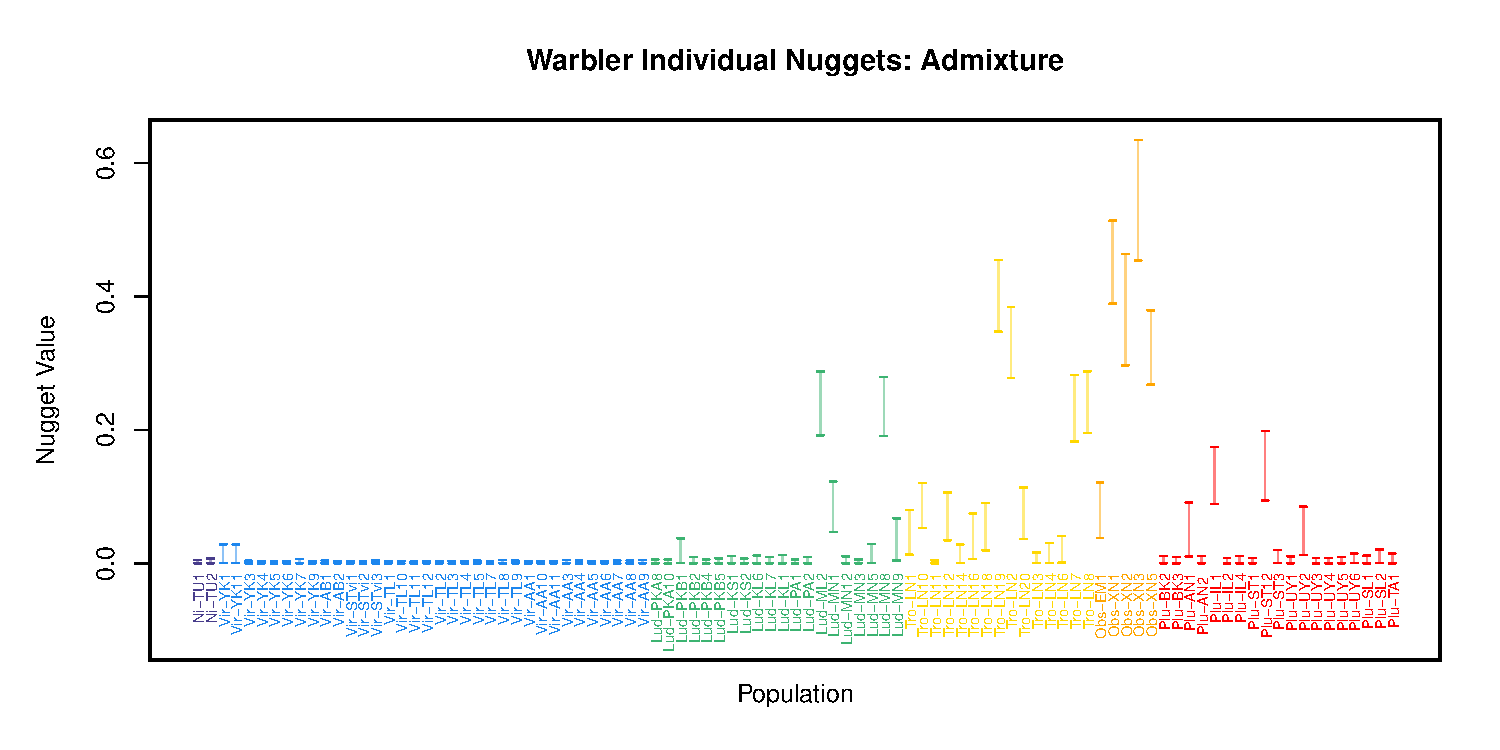
\includegraphics[width=5in,height=2.5in]{figs/warblers/warb_ind_Ad_nugget.pdf}}
	\caption{Credible intervals on estimated warbler individual nugget parameters in an analysis with admixture.}\label{sfig:warb_ind_ad_nugg}
\end{figure}

\begin{figure}
\centering
	{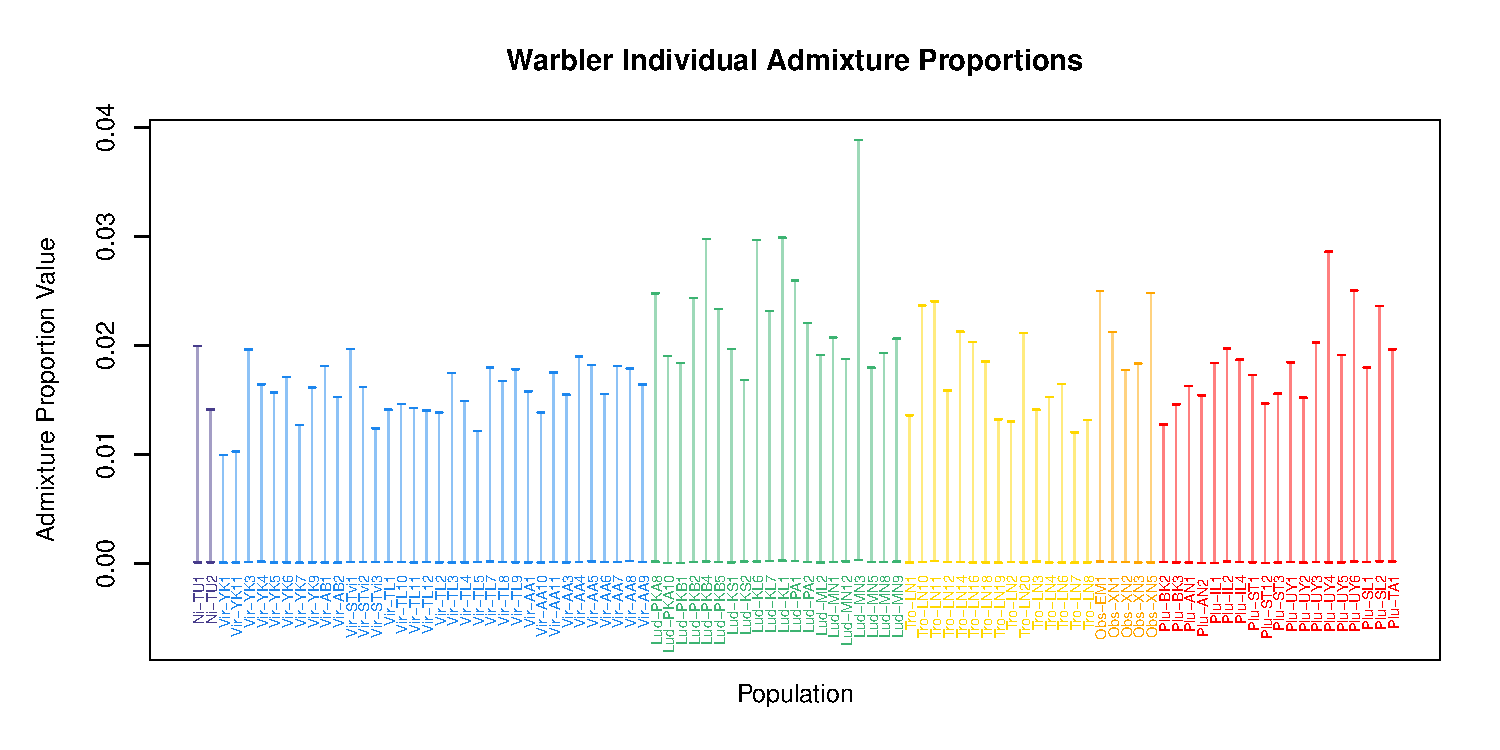
\includegraphics[width=5in,height=2.5in]{figs/warblers/warb_ind_adprop.pdf}}
	\caption{Credible intervals on estimated warbler individual admixture proportion parameters.}\label{sfig:warb_ind_adprops}
\end{figure}

\begin{figure}
	\centering
		\subcaptionbox{All population pairs \label{warb_ind_dist_compare_allpairs}}
			{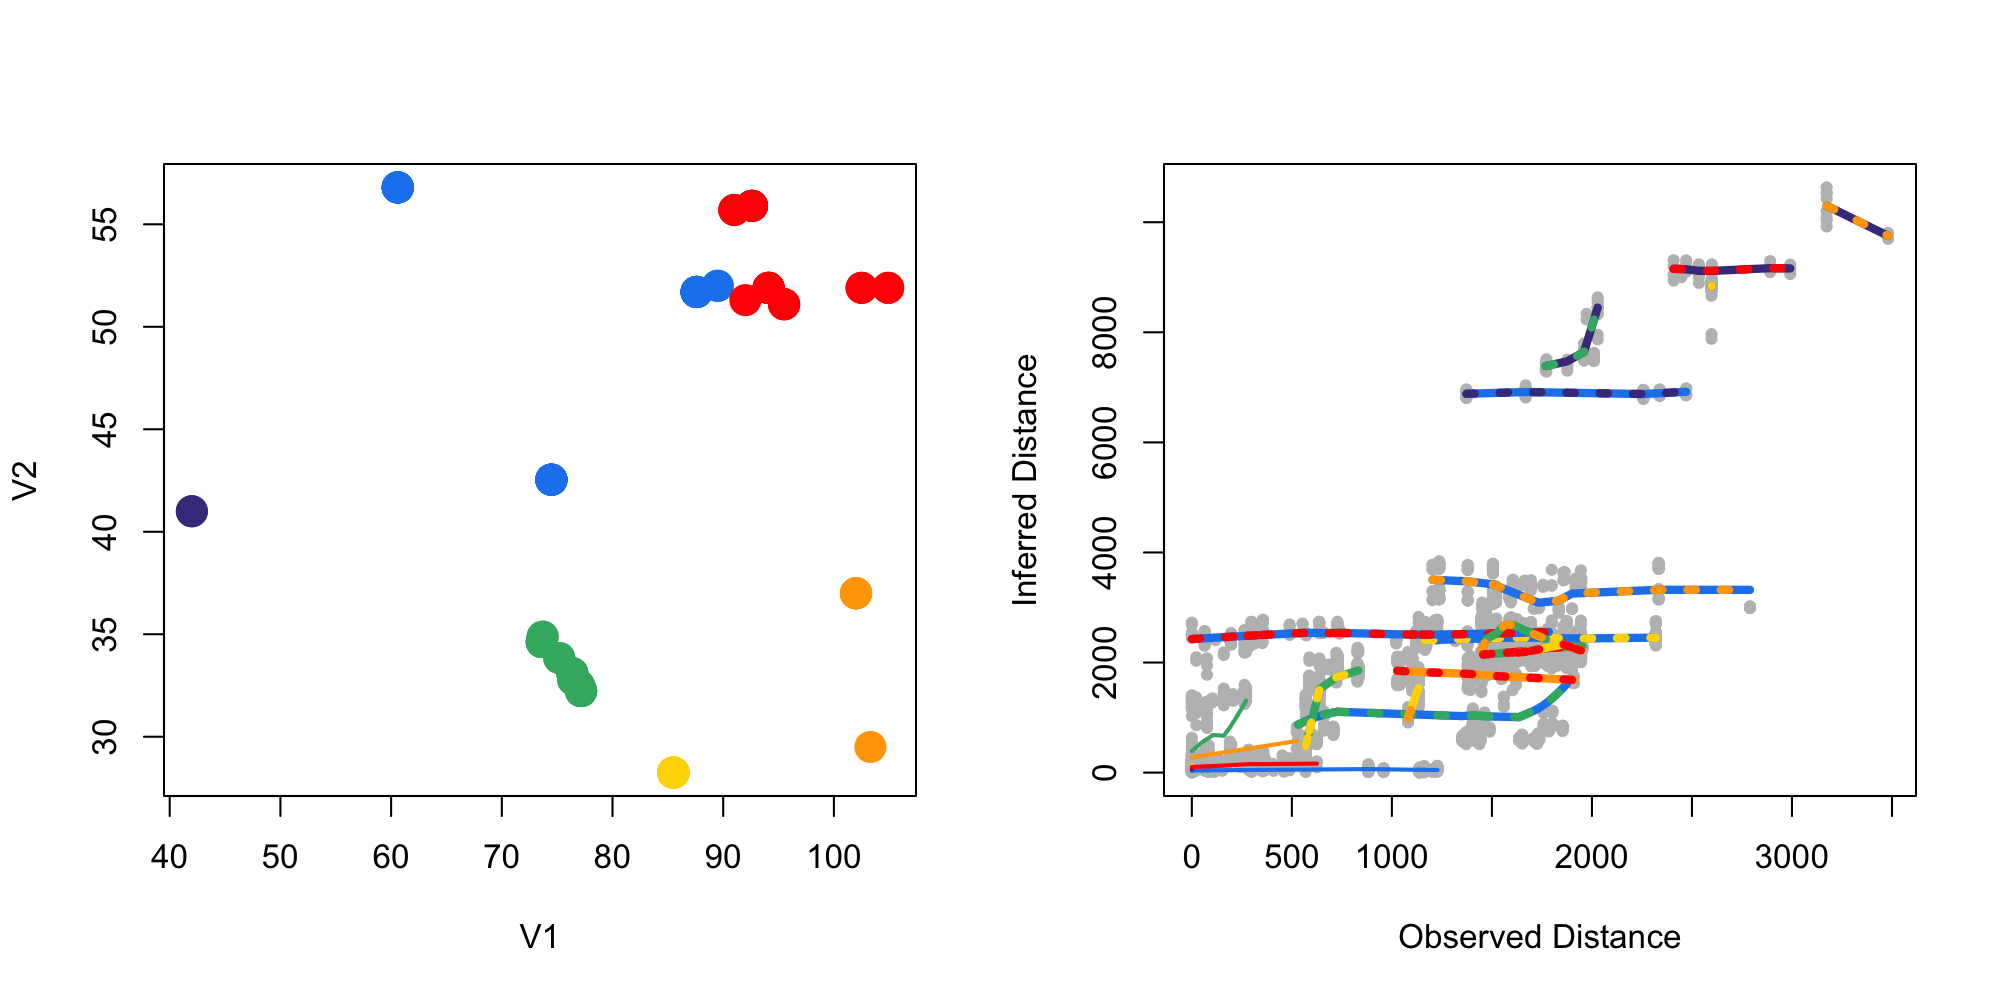
\includegraphics[width=6in,height=3in]{figs/warblers/warb_ind_dist_compare_allpairs.png}}
		\subcaptionbox{Just within population comparisons \label{warb_ind_dist_compare}}
			{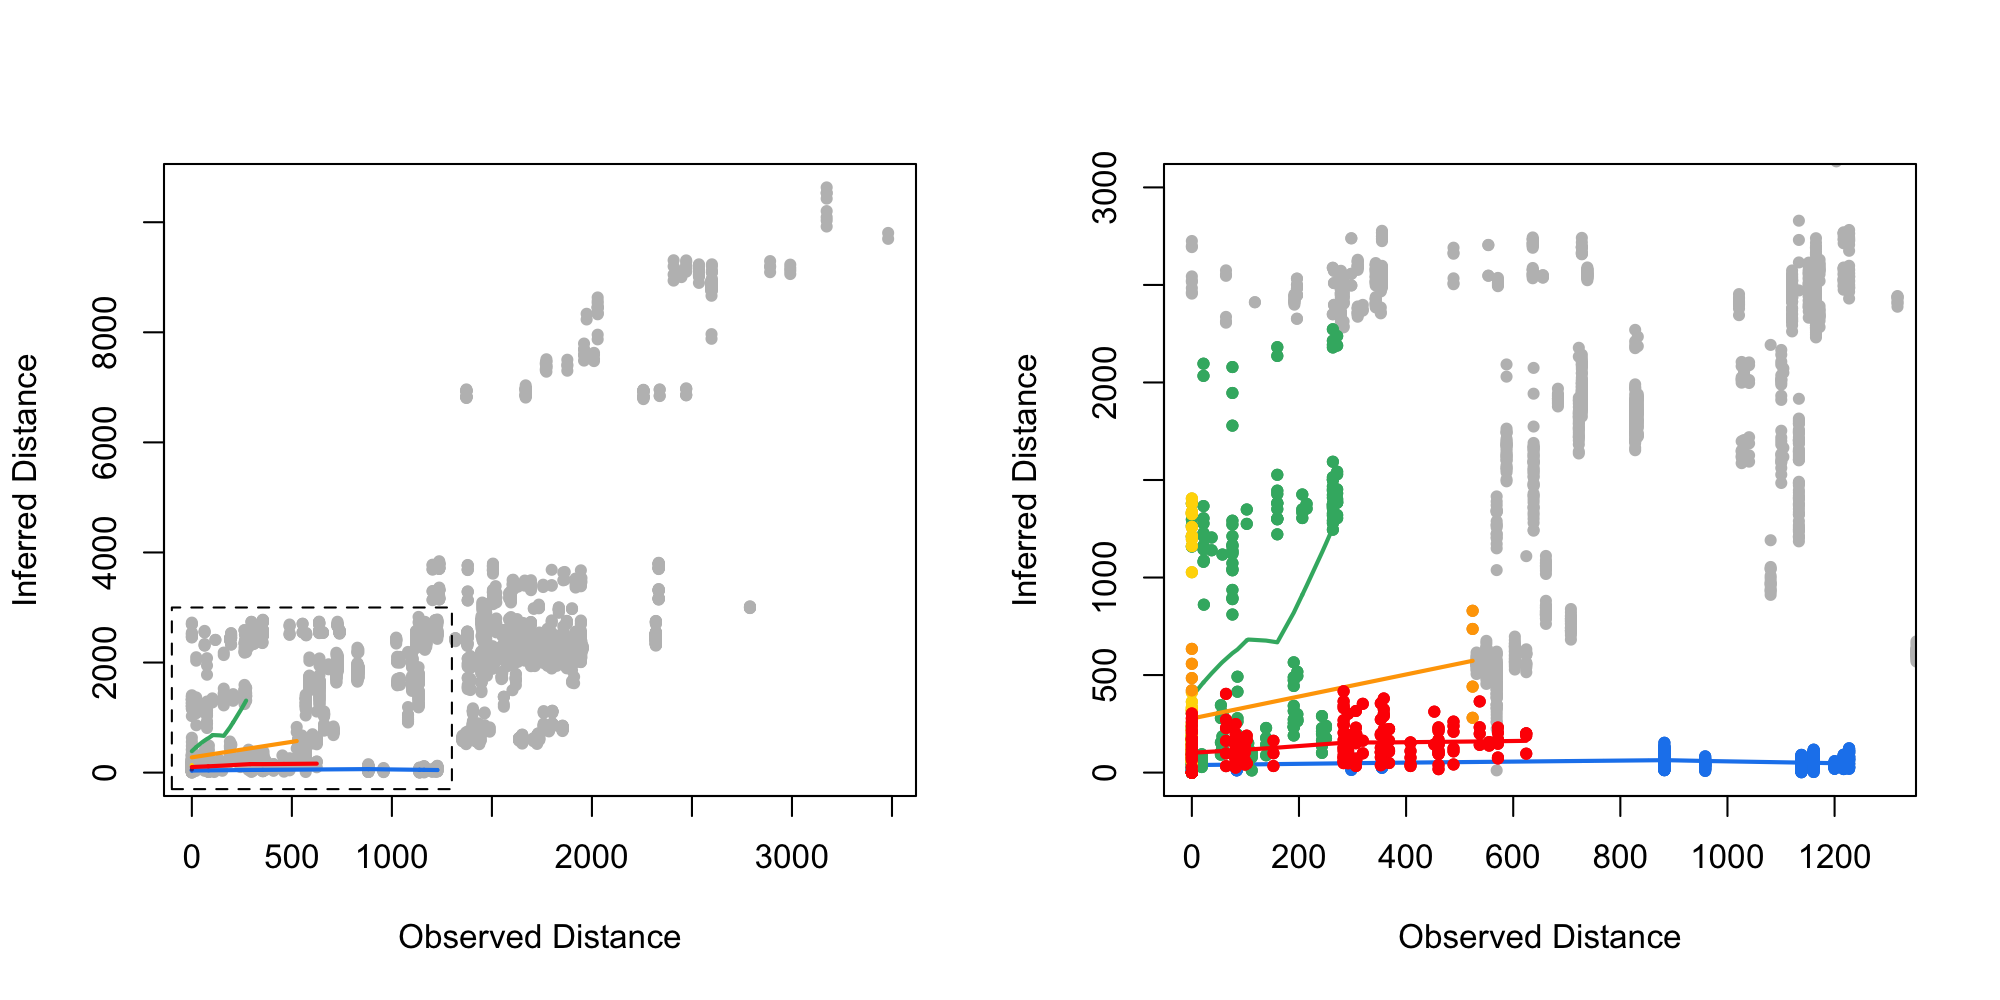
\includegraphics[width=6in,height=3in]{figs/warblers/warb_ind_dist_compare.png}}
	\caption{Comparing observed to estimated pairwise distance between warbler individuals, (a) between and (b) within subspecies populations.}\label{sfig:warb_ind_distcomp}
\end{figure}

\begin{figure}
\centering
	{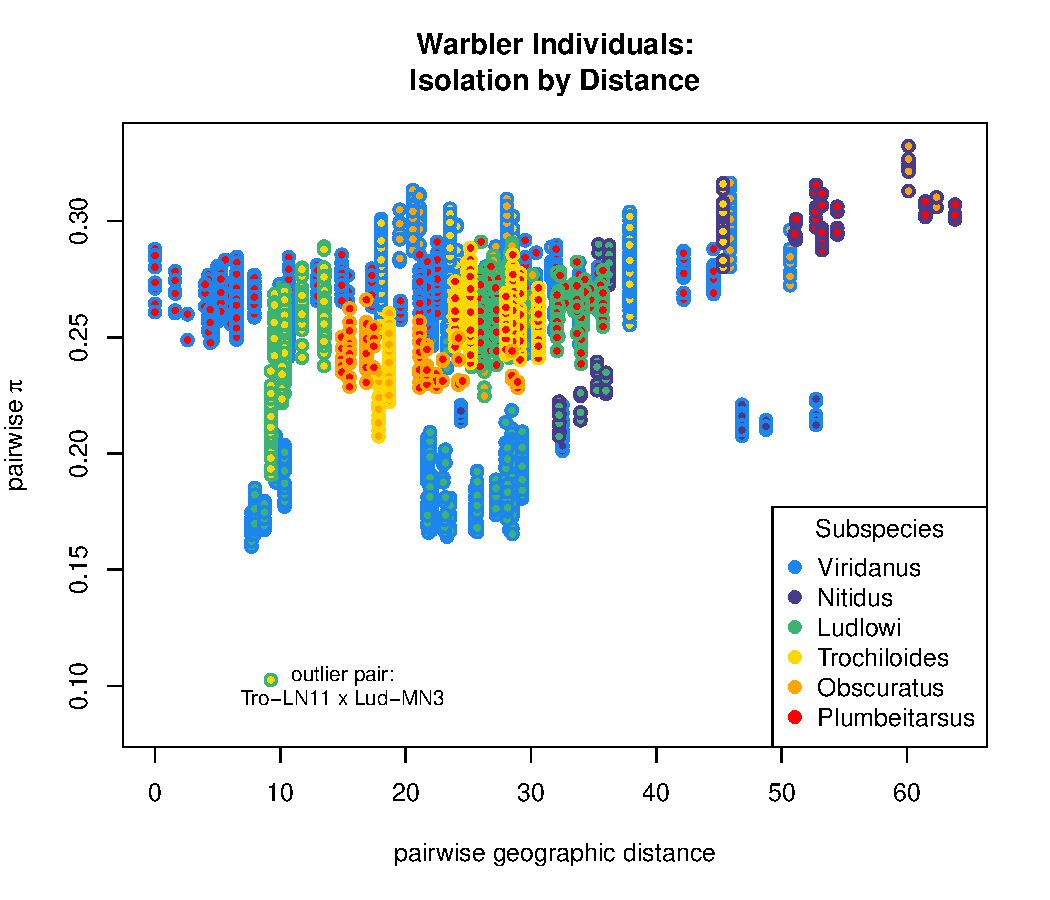
\includegraphics[width=5in,height=4.3in]{figs/warblers/warb_ind_pairwise_pi.pdf}}
	\caption{Pairwise $\pi$ at polymorphic sites calculated between all pairs of individuals from different subspecies, and colored by the subspecies to which each individual in the comparison is drawn.  Note that individuals Tro-LN11 and Lud-MN3 have sequence divergence that is unusually low relative to that of other comparisons between individuals from the same two subspecies.}\label{sfig:warb_ind_pwp}
\end{figure}

\begin{figure}
	\centering
		\subcaptionbox{warbler individuals projected onto a line \label{warb_ind_line_setup}}
			{\includegraphics[width=2.8in,height=2.33in]{figs/warblers/warb_inds_on_a_line_setup.pdf}}
		\subcaptionbox{MAP estimate from SpaceMix \label{warb_inds_line_MAP}}
			{\includegraphics[width=2.8in,height=2.33in]{figs/warblers/warb_inds_on_a_line_MAP1.pdf}}
		\subcaptionbox{Posterior distribution of locations from SpaceMix \label{warb_inds_line_post}}
			{\includegraphics[width=2.8in,height=2.33in]{figs/warblers/warb_inds_on_a_line_post1.pdf}}
	\caption{SpaceMix analyses performed on a warbler individuals for which prior locations are projected onto a flat line in an order that approximately corresponds to their order around the ring: a) the setup of the analysis, in which warbler individuals are projected from their estimated locations in a previous SpaceMix run onto a flat line; b) the MAP estimate of individual locations from a SpaceMix analysis with no admixture, using the flat line locations from (a) as priors on $G^{\prime}$; c) posterior distribution of individual locations from the same analysis.  As with the other inferred maps, here, for clarity, the inferred locations have been rotated via a Procrustes superimposition around their true sampling coordinates.}
	\label{sfig:warb_inds_on_a_line}
\end{figure}

\begin{figure}
\centering
	{\includegraphics[width=5in,height=2.5in]{figs/globetrotter/globe_NoAd_nugget.pdf}}
	\caption{Credible intervals on estimated human sample nugget parameters in an analysis without admixture.}\label{sfig:globe_noad_nugg}
\end{figure}

\begin{figure}
\centering
	{\includegraphics[width=5in,height=2.5in]{figs/globetrotter/globe_Ad_nugget.pdf}}
	\caption{Credible intervals on estimated human sample nugget parameters in an analysis with admixture.}\label{sfig:globe_ad_nugg}
\end{figure}

\clearpage

\begin{figure}
\centering
	{\includegraphics[width=5in,height=2.5in]{figs/globetrotter/globe_adprop.pdf}}
	\caption{Credible intervals on estimated human sample admixture proportion parameters.}\label{sfig:globe_adprops}
\end{figure}

\clearpage

\begin{figure}
	\centering
		{\includegraphics[width=6in,height=2.5in]{figs/globetrotter/globe_NoAd_dist_decay.png}} %globe_NoAd_dist_compare.png
	\caption{Comparison of observed distance to estimated distance between human populations, colored by continent from which populations were sampled (i.e.\ - two populations sampled from Africa are green).  Eurasia is divided into Western Eurasia and East Asia.}
\label{sfig:globe_noad_distcomp}
\end{figure}

\clearpage

\begin{figure}
	\centering
		\subcaptionbox{populations on a line \label{line_scenario}}
			{\includegraphics[width=3in,height=1.5in]{figs/sims/line_pops_scenario.pdf}}
		\subcaptionbox{PCA map of line scenario \label{line_pops_pca}}
			{\includegraphics[width=2.33in,height=2.33in]{figs/sims/line_pops_PCA.pdf}}
		\subcaptionbox{posterior from SpaceMix map of line scenario \label{line_pops_post}}
			{\includegraphics[width=3in,height=1.5in]{figs/sims/line_pops_inference_post.pdf}}
		\subcaptionbox{MAP estimate from SpaceMix map of line scenario \label{line_pops_MAP}}
			{\includegraphics[width=3in,height=1.5in]{figs/sims/line_pops_inference_MAP.pdf}}
	\caption{Simulation scenario of populations on a line, contrasting PCA-based inference and SpaceMix inference. a) Scenario used to simulate data in a spatial coalescent framework with nearest-neighbor migration; b) PCA map of allele frequencies, plotting PC axis 1 against PC axis 2, forming a `U' shape; c) Posterior distribution of SpaceMix location inference, forming a rough line; d) snapshot of the MAP draw from the posterior, again showing a rough line.}
	\label{sfig:line_scenario}
\end{figure}

\begin{figure}
	\centering
		{\includegraphics[width=6in,height=2.5in]{figs/sims/example_acceptance_rates.png}}
	\caption{Example parameter acceptance proportions for the $\alpha_2$ parameter and the nugget parameter, $\eta$, using the adaptive Metropolis-within-Gibbs proposal mechanism.}\label{sfig:example_acceptance_rates}
\end{figure}

\clearpage

\begin{table}
\centering
\tiny
\begin{tabular}{rlrr}
  \hline
Sample & Subspecies & Longitude & Latitude \\ 
  \hline
 Vir-YK1 & \textcolor{blue}{Viridanus} & 60.60 & 60.60 \\ 
   Vir-YK11 & \textcolor{blue}{Viridanus} & 60.60 & 60.60 \\ 
   Vir-YK3 & \textcolor{blue}{Viridanus} & 60.60 & 60.60 \\ 
   Vir-YK4 & \textcolor{blue}{Viridanus} & 60.60 & 60.60 \\ 
   Vir-YK5 & \textcolor{blue}{Viridanus} & 60.60 & 60.60 \\ 
   Vir-YK6 & \textcolor{blue}{Viridanus} & 60.60 & 60.60 \\ 
   Vir-YK7 & \textcolor{blue}{Viridanus} & 60.60 & 60.60 \\ 
   Vir-YK9 & \textcolor{blue}{Viridanus} & 60.60 & 60.60 \\ 
   Vir-AB1 & \textcolor{blue}{Viridanus} & 89.50 & 89.50 \\ 
   Vir-AB2 & \textcolor{blue}{Viridanus} & 89.50 & 89.50 \\ 
  Vir-STvi1 & \textcolor{blue}{Viridanus} & 92.60 & 92.60 \\ 
  Vir-STvi2 & \textcolor{blue}{Viridanus} & 92.60 & 92.60 \\ 
  Vir-STvi3 & \textcolor{blue}{Viridanus} & 92.60 & 92.60 \\ 
   Vir-TL1 & \textcolor{blue}{Viridanus} & 87.60 & 87.60 \\ 
   Vir-TL10 & \textcolor{blue}{Viridanus} & 87.60 & 87.60 \\ 
   Vir-TL11 & \textcolor{blue}{Viridanus} & 87.60 & 87.60 \\ 
   Vir-TL12 & \textcolor{blue}{Viridanus} & 87.60 & 87.60 \\ 
   Vir-TL2 & \textcolor{blue}{Viridanus} & 87.60 & 87.60 \\ 
   Vir-TL3 & \textcolor{blue}{Viridanus} & 87.60 & 87.60 \\ 
   Vir-TL4 & \textcolor{blue}{Viridanus} & 87.60 & 87.60 \\ 
   Vir-TL5 & \textcolor{blue}{Viridanus} & 87.60 & 87.60 \\ 
   Vir-TL7 & \textcolor{blue}{Viridanus} & 87.60 & 87.60 \\ 
   Vir-TL8 & \textcolor{blue}{Viridanus} & 87.60 & 87.60 \\ 
   Vir-TL9 & \textcolor{blue}{Viridanus} & 87.60 & 87.60 \\ 
   Vir-AA1 & \textcolor{blue}{Viridanus} & 74.48 & 74.48 \\ 
   Vir-AA10 & \textcolor{blue}{Viridanus} & 74.48 & 74.48 \\ 
   Vir-AA11 & \textcolor{blue}{Viridanus} & 74.48 & 74.48 \\ 
   Vir-AA3 & \textcolor{blue}{Viridanus} & 74.48 & 74.48 \\ 
   Vir-AA4 & \textcolor{blue}{Viridanus} & 74.48 & 74.48 \\ 
   Vir-AA5 & \textcolor{blue}{Viridanus} & 74.48 & 74.48 \\ 
   Vir-AA6 & \textcolor{blue}{Viridanus} & 74.48 & 74.48 \\ 
   Vir-AA7 & \textcolor{blue}{Viridanus} & 74.48 & 74.48 \\ 
   Vir-AA8 & \textcolor{blue}{Viridanus} & 74.48 & 74.48 \\ 
   Vir-AA9 & \textcolor{blue}{Viridanus} & 74.48 & 74.48 \\ 
   \hline
   Ni-TU1 & \textcolor{BlueViolet}{Nitidus} & 42.00 & 42.00 \\ 
   Ni-TU2 & \textcolor{BlueViolet}{Nitidus} & 42.00 & 42.00 \\ 
      \hline
   Lud-PKA8 & \textcolor{ForestGreen}{Ludlowi} & 73.69 & 73.69 \\ 
   Lud-PKA10 & \textcolor{ForestGreen}{Ludlowi} & 73.69 & 73.69 \\ 
   Lud-PKB1 & \textcolor{ForestGreen}{Ludlowi} & 73.61 & 73.61 \\ 
   Lud-PKB2 & \textcolor{ForestGreen}{Ludlowi} & 73.61 & 73.61 \\ 
   Lud-PKB4 & \textcolor{ForestGreen}{Ludlowi} & 73.61 & 73.61 \\ 
   Lud-PKB5 & \textcolor{ForestGreen}{Ludlowi} & 73.61 & 73.61 \\ 
   Lud-KS1 & \textcolor{ForestGreen}{Ludlowi} & 75.19 & 75.19 \\ 
   Lud-KS2 & \textcolor{ForestGreen}{Ludlowi} & 75.19 & 75.19 \\ 
   Lud-KL6 & \textcolor{ForestGreen}{Ludlowi} & 76.37 & 76.37 \\ 
   Lud-KL7 & \textcolor{ForestGreen}{Ludlowi} & 76.37 & 76.37 \\ 
   Lud-KL1 & \textcolor{ForestGreen}{Ludlowi} & 76.37 & 76.37 \\ 
   Lud-PA1 & \textcolor{ForestGreen}{Ludlowi} & 76.97 & 76.97 \\ 
   Lud-PA2 & \textcolor{ForestGreen}{Ludlowi} & 76.97 & 76.97 \\ 
   Lud-ML2 & \textcolor{ForestGreen}{Ludlowi} & 76.43 & 76.43 \\ 
   Lud-MN1 & \textcolor{ForestGreen}{Ludlowi} & 77.16 & 77.16 \\ 
   Lud-MN12 & \textcolor{ForestGreen}{Ludlowi} & 77.16 & 77.16 \\ 
   Lud-MN3 & \textcolor{ForestGreen}{Ludlowi} & 77.16 & 77.16 \\ 
   Lud-MN5 & \textcolor{ForestGreen}{Ludlowi} & 77.16 & 77.16 \\ 
   Lud-MN8 & \textcolor{ForestGreen}{Ludlowi} & 77.16 & 77.16 \\ 
   Lud-MN9 & \textcolor{ForestGreen}{Ludlowi} & 77.16 & 77.16 \\ 
      \hline
   Tro-LN1 & \textcolor{Goldenrod}{Trochiloides} & 85.50 & 85.50 \\ 
   Tro-LN10 & \textcolor{Goldenrod}{Trochiloides} & 85.50 & 85.50 \\ 
   Tro-LN11 & \textcolor{Goldenrod}{Trochiloides} & 85.50 & 85.50 \\ 
   Tro-LN12 & \textcolor{Goldenrod}{Trochiloides} & 85.50 & 85.50 \\ 
   Tro-LN14 & \textcolor{Goldenrod}{Trochiloides} & 85.50 & 85.50 \\ 
   Tro-LN16 & \textcolor{Goldenrod}{Trochiloides} & 85.50 & 85.50 \\ 
   Tro-LN18 & \textcolor{Goldenrod}{Trochiloides} & 85.50 & 85.50 \\ 
   Tro-LN19 & \textcolor{Goldenrod}{Trochiloides} & 85.50 & 85.50 \\ 
   Tro-LN2 & \textcolor{Goldenrod}{Trochiloides} & 85.50 & 85.50 \\ 
   Tro-LN20 & \textcolor{Goldenrod}{Trochiloides} & 85.50 & 85.50 \\ 
   Tro-LN3 & \textcolor{Goldenrod}{Trochiloides} & 85.50 & 85.50 \\ 
   Tro-LN4 & \textcolor{Goldenrod}{Trochiloides} & 85.50 & 85.50 \\ 
   Tro-LN6 & \textcolor{Goldenrod}{Trochiloides} & 85.50 & 85.50 \\ 
   Tro-LN7 & \textcolor{Goldenrod}{Trochiloides} & 85.50 & 85.50 \\ 
   Tro-LN8 & \textcolor{Goldenrod}{Trochiloides} & 85.50 & 85.50 \\ 
      \hline
   Obs-EM1 & \textcolor{BurntOrange}{Obscuratus} & 103.30 & 103.30 \\ 
   Obs-XN1 & \textcolor{BurntOrange}{Obscuratus} & 102.00 & 102.00 \\ 
   Obs-XN2 & \textcolor{BurntOrange}{Obscuratus} & 102.00 & 102.00 \\ 
   Obs-XN3 & \textcolor{BurntOrange}{Obscuratus} & 102.00 & 102.00 \\ 
   Obs-XN5 & \textcolor{BurntOrange}{Obscuratus} & 102.00 & 102.00 \\ 
      \hline
   Plu-BK2 & \textcolor{red}{Plumbeitarsus} & 104.90 & 104.90 \\ 
   Plu-BK3 & \textcolor{red}{Plumbeitarsus} & 104.90 & 104.90 \\ 
   Plu-AN1 & \textcolor{red}{Plumbeitarsus} & 102.50 & 102.50 \\ 
   Plu-AN2  & \textcolor{red}{Plumbeitarsus} & 102.50 & 102.50 \\ 
   Plu-IL1 & \textcolor{red}{Plumbeitarsus} & 95.50 & 95.50 \\ 
   Plu-IL2 & \textcolor{red}{Plumbeitarsus} & 95.50 & 95.50 \\ 
   Plu-IL4 & \textcolor{red}{Plumbeitarsus} & 95.50 & 95.50 \\ 
   Plu-ST1 & \textcolor{red}{Plumbeitarsus} & 92.60 & 92.60 \\ 
   Plu-ST12 & \textcolor{red}{Plumbeitarsus} & 92.60 & 92.60 \\ 
   Plu-ST3 & \textcolor{red}{Plumbeitarsus} & 92.60 & 92.60 \\ 
   Plu-UY1 & \textcolor{red}{Plumbeitarsus} & 94.10 & 94.10 \\ 
   Plu-UY2 & \textcolor{red}{Plumbeitarsus} & 94.10 & 94.10 \\ 
   Plu-UY3 & \textcolor{red}{Plumbeitarsus} & 94.10 & 94.10 \\ 
   Plu-UY4 & \textcolor{red}{Plumbeitarsus} & 94.10 & 94.10 \\ 
   Plu-UY5 & \textcolor{red}{Plumbeitarsus} & 94.10 & 94.10 \\ 
   Plu-UY6 & \textcolor{red}{Plumbeitarsus} & 94.10 & 94.10 \\ 
   Plu-SL1 & \textcolor{red}{Plumbeitarsus} & 91.00 & 91.00 \\ 
   Plu-SL2 & \textcolor{red}{Plumbeitarsus} & 91.00 & 91.00 \\ 
   Plu-TA1 & \textcolor{red}{Plumbeitarsus} & 92.00 & 92.00 \\ 
   \hline
   \end{tabular}
   \caption{Subspecies and geographic meta-data for greenish warbler individuals included in analysis}
   \label{tab:warbler_data_table}
\end{table}


 \definecolor{Adygei}{HTML}{4B00FF} 
 \definecolor{Armenian}{HTML}{6200FF} 
 \definecolor{Balochi}{HTML}{B400FF} 
 \definecolor{BantuKenya}{HTML}{00FF12} 
 \definecolor{BantuSouthAfrica}{HTML}{ADFF00} 
 \definecolor{Basque}{HTML}{0047FF} 
 \definecolor{Bedouin}{HTML}{3600FF} 
 \definecolor{Belorussian}{HTML}{2200FF} 
 \definecolor{BiakaPygmy}{HTML}{00FF72} 
 \definecolor{Brahui}{HTML}{AD00FF} 
 \definecolor{Bulgarian}{HTML}{1800FF} 
 \definecolor{Burusho}{HTML}{CE00FF} 
 \definecolor{Cambodian}{HTML}{FF00BC} 
 \definecolor{Chuvash}{HTML}{7500FF} 
 \definecolor{Colombian}{HTML}{FF9800} 
 \definecolor{Cypriot}{HTML}{3600FF} 
 \definecolor{Dai}{HTML}{FF00D2} 
 \definecolor{Daur}{HTML}{FF0074} 
 \definecolor{Druze}{HTML}{4300FF} 
 \definecolor{EastSicilian}{HTML}{000BFF} 
 \definecolor{Egyptian}{HTML}{006CFF} 
 \definecolor{English}{HTML}{004AFF} 
 \definecolor{Ethiopian}{HTML}{00FCFF} 
 \definecolor{EthiopianJew}{HTML}{009CFF} 
 \definecolor{Finnish}{HTML}{1900FF} 
 \definecolor{French}{HTML}{0040FF} 
 \definecolor{Georgian}{HTML}{6000FF} 
 \definecolor{GermanyAustria}{HTML}{0020FF} 
 \definecolor{Greek}{HTML}{0A00FF} 
 \definecolor{Hadza}{HTML}{1EFF00} 
 \definecolor{Han}{HTML}{FF009A} 
 \definecolor{HanNchina}{HTML}{FF00B0} 
 \definecolor{Hazara}{HTML}{BD00FF} 
 \definecolor{Hezhen}{HTML}{FF0053} 
 \definecolor{Hungarian}{HTML}{0200FF} 
 \definecolor{IndianJew}{HTML}{CA00FF} 
 \definecolor{Indian}{HTML}{DC00FF} 
 \definecolor{Myanmar}{HTML}{FF00DD} 
 \definecolor{Iranian}{HTML}{8200FF} 
 \definecolor{Ireland}{HTML}{0066FF} 
 \definecolor{Japanese}{HTML}{FF0040} 
 \definecolor{Jordanian}{HTML}{4300FF} 
 \definecolor{Kalash}{HTML}{C300FF} 
 \definecolor{Karitiana}{HTML}{FFA600} 
 \definecolor{Lahu}{HTML}{FF00CA} 
 \definecolor{Lezgin}{HTML}{6B00FF} 
 \definecolor{Lithuanian}{HTML}{1200FF} 
 \definecolor{Makrani}{HTML}{A900FF} 
 \definecolor{Mandenka}{HTML}{00CCFF} 
 \definecolor{Maya}{HTML}{FF5B00} 
 \definecolor{MbutiPygmy}{HTML}{00FF42} 
 \definecolor{Melanesian}{HTML}{FF0000} 
 \definecolor{Miao}{HTML}{FF00B0} 
 \definecolor{Mongola}{HTML}{FF0087} 
 \definecolor{Moroccan}{HTML}{000CFF} 
 \definecolor{Mozabite}{HTML}{003CFF} 
 \definecolor{Naxi}{HTML}{FF00CE} 
 \definecolor{NorthItalian}{HTML}{0023FF} 
 \definecolor{Norwegian}{HTML}{0027FF} 
 \definecolor{Orcadian}{HTML}{0053FF} 
 \definecolor{Oroqen}{HTML}{FF006D} 
 \definecolor{Palestinian}{HTML}{3C00FF} 
 \definecolor{Papuan}{HTML}{FF002D} 
 \definecolor{Pathan}{HTML}{C900FF} 
 \definecolor{Pima}{HTML}{FF2E00} 
 \definecolor{Polish}{HTML}{0000FF} 
 \definecolor{Romanian}{HTML}{1600FF} 
 \definecolor{Russian}{HTML}{4F00FF} 
 \definecolor{Sandawe}{HTML}{00FFA2} 
 \definecolor{SanNamibia}{HTML}{4EFF00} 
 \definecolor{SanKhomani}{HTML}{7DFF00} 
 \definecolor{Sardinian}{HTML}{0026FF} 
 \definecolor{Saudi}{HTML}{6200FF} 
 \definecolor{Scottish}{HTML}{0057FF} 
 \definecolor{She}{HTML}{FF0087} 
 \definecolor{Sindhi}{HTML}{BC00FF} 
 \definecolor{SouthItalian}{HTML}{0008FF} 
 \definecolor{Spanish}{HTML}{0055FF} 
 \definecolor{Surui}{HTML}{FFA800} 
 \definecolor{Syrian}{HTML}{4B00FF} 
 \definecolor{Tu}{HTML}{FF00CA} 
 \definecolor{Tujia}{HTML}{FF00A9} 
 \definecolor{Tunisian}{HTML}{2400FF} 
 \definecolor{Turkish}{HTML}{3D00FF} 
 \definecolor{Tuscan}{HTML}{001EFF} 
 \definecolor{UAE}{HTML}{8500FF} 
 \definecolor{Uygur}{HTML}{E900FF} 
 \definecolor{Uzbekistani}{HTML}{AB00FF} 
 \definecolor{Welsh}{HTML}{0055FF} 
 \definecolor{WestSicilian}{HTML}{0018FF} 
 \definecolor{Xibo}{HTML}{E900FF} 
 \definecolor{Yakut}{HTML}{FF0062} 
 \definecolor{Yemeni}{HTML}{6F00FF} 
 \definecolor{Yi}{HTML}{FF00C3} 
 \definecolor{Yoruba}{HTML}{00FFD2}
 
 
 \begin{table}[ht]
 \tiny
\centering
\begin{tabular}{rlrrr}
  \hline
 & Population & Longitude & Latitude & Mean Sample Size \\ 
  \hline
1 & \textcolor{BantuSouthAfrica}{BantuSouthAfrica} & 28.00 & -26.00 & 15.99 \\ 
  2 & \textcolor{SanKhomani}{SanKhomani} & 18.10 & -24.60 & 59.96 \\ 
  3 & \textcolor{SanNamibia}{SanNamibia} & 20.00 & -21.50 & 9.99 \\ 
  4 & \textcolor{Hadza}{Hadza} & 33.10 & -4.50 & 5.93 \\ 
  5 & \textcolor{BantuKenya}{BantuKenya} & 37.00 & -3.00 & 21.99 \\ 
  6 & \textcolor{MbutiPygmy}{MbutiPygmy} & 29.00 & 1.00 & 25.98 \\ 
  7 & \textcolor{BiakaPygmy}{BiakaPygmy} & 17.00 & 4.00 & 41.97 \\ 
  8 & \textcolor{Sandawe}{Sandawe} & 35.70 & 6.20 & 55.94 \\ 
  9 & \textcolor{Yoruba}{Yoruba} & 5.00 & 8.00 & 41.98 \\ 
  10 & \textcolor{Ethiopian}{Ethiopian} & 38.70 & 9.00 & 37.70 \\ 
  11 & \textcolor{Mandenka}{Mandenka} & -12.00 & 12.00 & 43.98 \\ 
  12 & \textcolor{EthiopianJew}{EthiopianJew} & 38.70 & 14.10 & 22.00 \\ 
  13 & \textcolor{Egyptian}{Egyptian} & 26.80 & 30.80 & 24.00 \\ 
  14 & \textcolor{Mozabite}{Mozabite} & 3.00 & 32.00 & 57.98 \\ 
  15 & \textcolor{Moroccan}{Moroccan} & -5.50 & 33.60 & 49.97 \\ 
  16 & \textcolor{Tunisian}{Tunisian} & 9.80 & 35.60 & 24.00 \\ 
  17 & \textcolor{Ireland}{Ireland} & -8.20 & 53.40 & 14.00 \\ 
  18 & \textcolor{Scottish}{Scottish} & -4.20 & 56.50 & 12.00 \\ 
  19 & \textcolor{Spanish}{Spanish} & -3.70 & 40.50 & 67.95 \\ 
  20 & \textcolor{Welsh}{Welsh} & -3.70 & 52.60 & 8.00 \\ 
  21 & \textcolor{Orcadian}{Orcadian} & -3.00 & 59.00 & 29.99 \\ 
  22 & \textcolor{English}{English} & -0.80 & 52.00 & 12.00 \\ 
  23 & \textcolor{Basque}{Basque} & 0.00 & 43.00 & 47.99 \\ 
  24 & \textcolor{French}{French} & 2.00 & 46.00 & 55.97 \\ 
  25 & \textcolor{Norwegian}{Norwegian} & 8.50 & 60.50 & 35.99 \\ 
  26 & \textcolor{Sardinian}{Sardinian} & 9.00 & 40.00 & 55.98 \\ 
  27 & \textcolor{NorthItalian}{NorthItalian} & 9.70 & 45.70 & 23.99 \\ 
  28 & \textcolor{GermanyAustria}{GermanyAustria} & 10.50 & 51.20 & 8.00 \\ 
  29 & \textcolor{Tuscan}{Tuscan} & 11.00 & 43.00 & 16.00 \\ 
  30 & \textcolor{WestSicilian}{WestSicilian} & 12.50 & 38.00 & 20.00 \\ 
  31 & \textcolor{EastSicilian}{EastSicilian} & 16.10 & 37.00 & 20.00 \\ 
  32 & \textcolor{SouthItalian}{SouthItalian} & 16.90 & 39.50 & 35.96 \\ 
  33 & \textcolor{Polish}{Polish} & 19.10 & 51.90 & 31.99 \\ 
  34 & \textcolor{Hungarian}{Hungarian} & 19.50 & 47.20 & 40.00 \\ 
  35 & \textcolor{Greek}{Greek} & 21.80 & 39.10 & 39.99 \\ 
  36 & \textcolor{Lithuanian}{Lithuanian} & 23.90 & 55.20 & 20.00 \\ 
  37 & \textcolor{Romanian}{Romanian} & 25.00 & 45.90 & 28.00 \\ 
  38 & \textcolor{Bulgarian}{Bulgarian} & 25.50 & 42.70 & 35.99 \\ 
  39 & \textcolor{Finnish}{Finnish} & 25.70 & 61.90 & 4.00 \\ 
  40 & \textcolor{Belorussian}{Belorussian} & 28.00 & 53.70 & 16.00 \\ 
  41 & \textcolor{Bedouin}{Bedouin} & 33.50 & 31.00 & 89.98 \\ 
  42 & \textcolor{Cypriot}{Cypriot} & 33.50 & 35.50 & 24.00 \\ 
  43 & \textcolor{Palestinian}{Palestinian} & 35.00 & 33.50 & 91.95 \\ 
  44 & \textcolor{Turkish}{Turkish} & 35.20 & 39.00 & 34.00 \\ 
  45 & \textcolor{Druze}{Druze} & 37.00 & 32.00 & 83.96 \\ 
  46 & \textcolor{Jordanian}{Jordanian} & 37.00 & 30.00 & 40.00 \\ 
  47 & \textcolor{Adygei}{Adygei} & 39.00 & 44.00 & 33.99 \\ 
  48 & \textcolor{Syrian}{Syrian} & 39.00 & 34.80 & 32.00 \\ 
  49 & \textcolor{Russian}{Russian} & 40.00 & 61.00 & 49.98 \\ 
  50 & \textcolor{Georgian}{Georgian} & 44.60 & 41.80 & 39.99 \\ 
  51 & \textcolor{Armenian}{Armenian} & 45.00 & 40.10 & 31.99 \\ 
  52 & \textcolor{Saudi}{Saudi} & 45.10 & 23.90 & 20.00 \\ 
  53 & \textcolor{Lezgin}{Lezgin} & 47.50 & 43.00 & 35.96 \\ 
  54 & \textcolor{Yemeni}{Yemeni} & 48.50 & 15.60 & 13.99 \\ 
  55 & \textcolor{Chuvash}{Chuvash} & 50.20 & 53.20 & 34.00 \\ 
  56 & \textcolor{Iranian}{Iranian} & 53.70 & 32.40 & 39.99 \\ 
  57 & \textcolor{UAE}{UAE} & 54.40 & 24.50 & 27.98 \\ 
  58 & \textcolor{Makrani}{Makrani} & 64.00 & 26.00 & 49.99 \\ 
  59 & \textcolor{Uzbekistani}{Uzbekistani} & 64.60 & 41.40 & 29.99 \\ 
  60 & \textcolor{Brahui}{Brahui} & 65.00 & 29.00 & 49.98 \\ 
  61 & \textcolor{Balochi}{Balochi} & 67.00 & 31.00 & 47.99 \\ 
  62 & \textcolor{Sindhi}{Sindhi} & 69.00 & 25.00 & 47.99 \\ 
  63 & \textcolor{Hazara}{Hazara} & 69.50 & 33.00 & 43.98 \\ 
  64 & \textcolor{Kalash}{Kalash} & 71.00 & 36.00 & 45.99 \\ 
  65 & \textcolor{Pathan}{Pathan} & 72.50 & 34.00 & 43.99 \\ 
  66 & \textcolor{IndianJew}{IndianJew} & 72.90 & 19.00 & 16.00 \\ 
  67 & \textcolor{Burusho}{Burusho} & 74.00 & 37.00 & 49.98 \\ 
  68 & \textcolor{Indian}{Indian} & 77.60 & 13.00 & 25.97 \\ 
  69 & \textcolor{Uygur}{Uygur} & 81.00 & 44.00 & 20.00 \\ 
  70 & \textcolor{Xibo}{Xibo} & 81.00 & 43.00 & 17.99 \\ 
  71 & \textcolor{Myanmar}{Myanmar} & 96.00 & 21.90 & 5.99 \\ 
  72 & \textcolor{Dai}{Dai} & 99.00 & 21.00 & 19.98 \\ 
  73 & \textcolor{Naxi}{Naxi} & 100.00 & 26.00 & 15.99 \\ 
  74 & \textcolor{Lahu}{Lahu} & 101.00 & 22.00 & 16.00 \\ 
  75 & \textcolor{Tu}{Tu} & 101.00 & 36.00 & 20.00 \\ 
  76 & \textcolor{Yi}{Yi} & 103.00 & 28.00 & 20.00 \\ 
  77 & \textcolor{Cambodian}{Cambodian} & 105.00 & 12.00 & 19.98 \\ 
  78 & \textcolor{HanNchina}{HanNchina} & 108.00 & 39.00 & 20.00 \\ 
  79 & \textcolor{Miao}{Miao} & 108.00 & 28.00 & 19.99 \\ 
  80 & \textcolor{Tujia}{Tujia} & 110.00 & 29.00 & 20.00 \\ 
  81 & \textcolor{Han}{Han} & 114.00 & 26.00 & 67.96 \\ 
  82 & \textcolor{Mongola}{Mongola} & 119.00 & 48.00 & 20.00 \\ 
  83 & \textcolor{She}{She} & 119.00 & 27.00 & 19.99 \\ 
  84 & \textcolor{Daur}{Daur} & 124.00 & 49.00 & 17.99 \\ 
  85 & \textcolor{Oroqen}{Oroqen} & 126.00 & 50.00 & 18.00 \\ 
  86 & \textcolor{Yakut}{Yakut} & 129.00 & 63.00 & 49.98 \\ 
  87 & \textcolor{Hezhen}{Hezhen} & 133.00 & 47.00 & 16.00 \\ 
  88 & \textcolor{Japanese}{Japanese} & 138.00 & 38.00 & 55.97 \\ 
  89 & \textcolor{Papuan}{Papuan} & 143.00 & -4.00 & 33.97 \\ 
  90 & \textcolor{Melanesian}{Melanesian} & 155.00 & -6.00 & 19.99 \\ 
  91 & \textcolor{Pima}{Pima} & -108.00 & 29.00 & 27.99 \\ 
  92 & \textcolor{Maya}{Maya} & -91.00 & 19.00 & 41.97 \\ 
  93 & \textcolor{Colombian}{Colombian} & -68.00 & 3.00 & 13.99 \\ 
  94 & \textcolor{Karitiana}{Karitiana} & -63.00 & -10.00 & 27.99 \\ 
  95 & \textcolor{Surui}{Surui} & -62.00 & -11.00 & 16.00 \\ 
   \hline
\end{tabular}
   \caption{sample size and geographic meta-data for human samples included in analysis}
   \label{tab:globe_data_table}
\end{table}


\end{document}


%%%%%%%%%%%%%%%%%%%%%%%%%%%%%%%%
%	TEXT GRAVEYARD
%%%%%%%%%%%%%%%%%%%%%%%%%%%%%%%%

%Isolation by distance is, in many ways, a more reasonable null hypothesis of population relatedness than a population phylogeny;  \gb{too compare-y?  should I ditch this?} population structure will only rarely be truly tree-like, and a strictly bifurcating graph is unable to accommodate many geographic scenarios, such as multiple equidistant populations in migration-drift equilibrium.

%, and we demonstrate the utility of this approach with two empirical applications.

%text for pairwise Pi plots!
To investigate the potential reason for this behavior, we calculated average pairwise sequence divergence at the 2,247 polymorphic loci in the dataset between all 95 individuals and plotted it against the pairwise geographic distance between the individuals (see SuppMat Figure NNN).  The pairwise sequence divergence (0.103) at polymorphic loci between Lud-MN3 and Tro-LN11 is significantly lower than that between any other pair of individuals separated by a comparable distance - lower, in fact, than any comparison between individuals that were not co-located, and lower than any pairwise divergence between any pair of individuals save that between the two Turkish \textit{nitidus} samples. 



 in which we estimate the 2-dimensional configuration of populations that, along with a model of the decay of covariance in allele frequencies with distance, best describes their empirical patterns of genetic differentiation
 
\subsection*{Spatial Admixture Statistic}

\subsection*{Modeling Admixture}
where $f_{\ell,i}$ is the allele frequency in population $i$, $f_{\ell,j}$ is the allele frequency in population $j$, and $p$ is the admixture proportion, which varies between 0 and 1 and describes the extent to which populations $i$ and $j$ are contributing to the genetic make-up of population $k$.

 To infer the spatial context of this admixture, we allow each population a point in space, which we refer to as its source of admixture, from which it draws its admixture, and we model both the location of that source and the extent (proportion) of that admixture.  The observed allele frequencies in sampled populations are therefore a weighted average of the model-estimated allele frequencies at the geographic location of the sampled population and those at the coordinates of the source from which the observed population draws admixture.  That is, the observed allele frequencies in population $k$ are modeled as follows:
 \begin{equation}
 f_{k} = pf_{k'} + (1-p)f_{j},
 \end{equation}
 where $f_{k'}$ are the model-estimated allele frequencies across loci at the spatial location of population $k$ and $f_{j}$ are the model-estimated allele frequencies at the spatial location of the source of admixture $j$, from which population $k$ is drawing admixture in proportion $p$.  The admixture proportion $p$ is constrained to vary between 0 and 0.5, such that at least half of a population's genetic make-up must be determined by its geographic location.

 We re-introduce the population-specific variance terms on each diagonal element of this admixed covariance matrix.  The full expression for our admixed covariance function is below.
 \begin{alignat}{3}
 \label{eq:admixed_covariance_2}
 \Omega^{(*)}_{i,j} = (1-p_i)(1-p_j) \Omega_{i\;,\;j\;} \; \times&\\
 (p_i)(1-p_j) \Omega_{i^{(*)},\;j\;} \; \times   \notag&\\
 (p_j)(1-p_i) \Omega_{i\;,\;j^{(*)}} \; \times   \notag&\\
 (p_i)(p_j) \Omega_{i^{(*)},\;j^{(*)}} \; +   \notag&\\
 \delta_{i,j} \bar{S_k}^{-1} + \delta_{i,j} \eta_k \phantom{+} \notag&
 \end{alignat}

 where $I$ is the identity matrix, $\bar{S_k}$ is the mean sample size in population $k$ across all loci, and $\eta_k$ is the nugget estimated in population $k$.

\section*{Inference}
For details on our Bayesian inference framework and Markov chain Monte Carlo inference procedure, please see the Section: How I spent the past year!

\begin{figure}
	\centering
		\subcaptionbox{Basic Lattice \label{basic_lattice}}
			{\includegraphics[width=3in,height=2.5in]{figs/sims/basic_lattice.png}}
		\subcaptionbox{Lattice with Barrier \label{barrier_lattice}}
			{\includegraphics[width=3in,height=2.5in]{figs/sims/barrier_lattice.png}}
		\subcaptionbox{Lattice with Expansion Event \label{barrier_lattice}}
			{\includegraphics[width=3in,height=2.5in]{figs/sims/expansion_lattice.png}}
	\caption{Different simulation scenarios: (a) basic lattice; (b) lattice with a longitudinal barrier; (c) lattice with expansion event.}\label{sfig:sim_scenarios}
\end{figure}

\begin{figure}[htp!]
	\centering
		{\includegraphics[width=2.4in,height=2in]{figs/sims/GeoGenMap_barr_inland_admixture_2.png}}
	\caption{credible interval of where population 23 draws admixture from.}
\label{sfig:barr_inland_ad_credset}
\end{figure}

\begin{figure}
	\centering
		\subcaptionbox{Lattice \label{lattice_inference}}
			{\includegraphics[width=2.8in,height=2.33in]{figs/sims/GeoGenMap_lattice.pdf}}
		\subcaptionbox{Barrier \label{barrier_inference}}
			{\includegraphics[width=2.8in,height=2.33in]{figs/sims/GeoGenMap_barrier.pdf}}
		\subcaptionbox{Expansion  \label{expansion_inference}}
			{\includegraphics[width=2.8in,height=2.33in]{figs/sims/GeoGenMap_expansion.pdf}}
		\subcaptionbox{Admixture \label{sfig:admixture_inference_CYOL}}
			{\includegraphics[width=2.8in,height=2.33in]{figs/sims/GeoGenMap_corner_admixture_CYOL.pdf}}
	\caption{Population maps inferred using SpaceMix under three different scenarios: a) simple lattice at equilibrium; b) a lattice with a barrier across the center line of longitude; c) a lattice with recent expansion on the eastern margin; d) a lattice with an admixture event between populations 1 and 30.}\label{sfig:lattice_scenarios}
\end{figure}


\begin{figure}
	\centering
		\subcaptionbox{Location Inference \label{sfig:admixture_inference_CYOL}}
			{\includegraphics[width=2.4in,height=2in]{figs/sims/GeoGenMap_corner_admixture_CYOL.pdf}}
		\subcaptionbox{Location and Admixture Inference \label{sfig:admixture_inference_CYOL}}
			{\includegraphics[width=2.4in,height=2in]{figs/sims/GeoGenMap_corner_admixture.png}}
	\caption{Inference of population locations in the scenario depicted in Figure \ref{sfig:admixture_scenario}.  Population 30 has received half of its lineages from population 1, to simulate a long distance admixture event in the very recent past. a) Inference of population locations; b) inference of both population locations and their sources of admixture}\label{sfig:corner_admixture_inference}
\end{figure}

\begin{figure}
	\centering
		\subcaptionbox{Lattice \label{lattice_inference}}
			{\includegraphics[width=2.8in,height=2.33in]{figs/sims/GeoGenMap_lattice.pdf}}
		\subcaptionbox{Barrier \label{barrier_inference}}
			{\includegraphics[width=2.8in,height=2.33in]{figs/sims/GeoGenMap_barrier.pdf}}
		\subcaptionbox{Expansion  \label{expansion_inference}}
			{\includegraphics[width=2.8in,height=2.33in]{figs/sims/GeoGenMap_expansion.pdf}}
		\subcaptionbox{Admixture \label{sfig:admixture_inference_CYOL}}
			{\includegraphics[width=2.8in,height=2.33in]{figs/sims/GeoGenMap_corner_admixture_CYOL.pdf}}
	\caption{Population maps inferred using SpaceMix under three different scenarios: a) simple lattice at equilibrium; b) a lattice with a barrier across the center line of longitude; c) a lattice with recent expansion on the eastern margin; d) a lattice with an admixture event between populations 1 and 30.}\label{sfig:lattice_scenarios}
\end{figure}


\begin{figure}
	\centering
		\subcaptionbox{Location Inference \label{sfig:admixture_inference_CYOL}}
			{\includegraphics[width=2.4in,height=2in]{figs/sims/GeoGenMap_corner_admixture_CYOL.pdf}}
		\subcaptionbox{Location and Admixture Inference \label{sfig:admixture_inference_CYOL}}
			{\includegraphics[width=2.4in,height=2in]{figs/sims/GeoGenMap_corner_admixture.png}}
	\caption{Inference of population locations in the scenario depicted in Figure \ref{sfig:admixture_scenario}.  Population 30 has received half of its lineages from population 1, to simulate a long distance admixture event in the very recent past. a) Inference of population locations; b) inference of both population locations and their sources of admixture}\label{sfig:corner_admixture_inference}
\end{figure}

\begin{figure}[htp!]
	\centering
	\includegraphics[width=2.4in,height=2in]{figs/sims/GeoGenMap_corner_admixture.png}
	\caption{Posterior distribution of inference of the sources and strengths of admixture for the sampled populations.  The admixed population (Population 30) is drawing admixture from the location of its source of admixture that was used to simulate the data (the location of Population 1).}\label{sfigGeoGenMap_corner_admixture}
\end{figure}


\begin{figure}
	\centering
		\subcaptionbox{Simulated Lattice \label{simple_lattice}}
			{\includegraphics[width=2.8in,height=2.33in]{figs/sims/basic_lattice.png}}
		\subcaptionbox{Lattice \label{lattice_inference}}
			{\includegraphics[width=2.8in,height=2.33in]{figs/sims/GeoGenMap_lattice.pdf}}
		\subcaptionbox{Barrier \label{barrier_inference}}
			{\includegraphics[width=2.8in,height=2.33in]{figs/sims/GeoGenMap_barrier.pdf}}
		\subcaptionbox{Expansion  \label{expansion_inference}}
			{\includegraphics[width=2.8in,height=2.33in]{figs/sims/GeoGenMap_expansion.pdf}}
	\caption{Population maps inferred using SpaceMix under three different scenarios: a) configuration of simulated populations; (c) simple lattice at equilibrium; c) a lattice with a barrier across the center line of longitude; d) a lattice with recent expansion on the eastern margin.}\label{sfig:lattice_scenarios}
\end{figure}
%%%Graham's attempts at arrows in equations
%\begin{equation}
%\source{A}~~~~B~~~~ \target{C}~~~~D
%\drawarrows
%\end{equation}
%blah blah

% \begin{equation}
%   A~~~~B\tikzmark{b} ~~~~ C~~~~\tikzmark{a}D
%   \tikz[overlay,remember picture]
%    {\draw[->,square arrow] (a.south) to (b.south);}
% \end{equation}
% blah blah
% \begin{equation}
%   A~~~~B\tikzmark{b} ~~~~ C~~~~\tikzmark{a}D
%   \tikz[overlay,remember picture]
%    {\draw[->,square arrow] (a.south) to (b.south);}
% \end{equation}
 
 
%\newcommand{\tikzmark}[1]{\tikz[overlay,remember picture] \node (#1) {};}
%\tikzset{square arrow/.style={to path={-- ++(0,-.25) -| (\tikztotarget)}}}

%\begin{equation}
 % a\tikzmark{a}x^2 + bx + c = 5\tikzmark{b}x^2 + bx + c.
 % \tikz[overlay,remember picture]
 %  {\draw[->,square arrow] (a.south) to (b.south);}
%\end{equation}


%%Graham's attempts at arrows in equations 
% \newcommand{\tikzmark}[1]{\tikz[overlay,remember picture] \node (#1) {};}
% \tikzset{square arrow/.style={to path={-- ++(0,-.25) -| (\tikztotarget)}}}


% \newcommand\source[1]{%
%     \tikz[remember picture,baseline,inner sep=0pt] {%
%         \node [name=source,anchor=base]{$#1$};
%     }%
%     \setcounter{target}{0}
% }

% \newcounter{target}
% \newcommand\target[1]{%
%     \tikz[remember picture,baseline,inner sep=0pt] {%
%         \node [name=target-\thetarget,anchor=base]{$#1$};
%     }%
%     \stepcounter{target}%
% }

% \newcommand\drawarrows{
%     \tikz[remember picture, overlay, bend left=20, -latex] {
%         \foreach \i [evaluate=\i as \n using int(\i-1)] in {1,...,\thetarget} {
%             \draw (source.north) to (target-\n.north);
%         }
%     }
% }


% \newcommand\newdrawarrows{
%     \tikz[remember picture, overlay, bend left=20, -latex] {
%         \foreach \i [evaluate=\i as \n using int(\i-1)] in {1,...,\thetarget} {
%             \draw (target-\n.north) to (source.north);
%         }
%     }
% }

% \gc{BLAH}
% Note, by using the sample mean frequency to mean-center our observations, we lose a degree of freedom, and reduce the covariance across loci between populations (sometimes inducing negative covariance between distant populations). We accommodate the extra sampling noise distortion and the reduced rank of the covariance matrix by assuming that our
% %
% \begin{equation}
% X_{\ell} \sim MVN(0, \Omega^{\prime} )
% \end{equation}
% %
% where $\Omega^{\prime}$ is a simple transform of $\Omega$.  Specifically, 
% %
% \begin{equation}
% \Omega^{\prime} = \Psi^{T}   \Omega   \Psi \text{,}
% \label{eq:projected_covariance}
% \end{equation}
% %
% where
%  %
% $\Psi$ is a projection matrix that is used to project our degenerate covariance matrix back into full rank.  This projection matrix is given by
% \begin{equation}
% \Psi = \text{qr.Q}(\text{qr}(\Upsilon))[,1:(k-1)] \text{,}
% \end{equation}
% %
% where $\text{qr}$ is the QR decomposition, $\text{qr.Q}$ returns the original matrix on which the QR decomposition was performed, and
%  $\Upsilon$, a matrix to mean-center the sample allele frequencies, weighting by the mean sample size in each population, is given by 
% \begin{equation}
% T_{ij} = \delta_{ij}  -  \frac{\bar{S}_j}{\sum\limits_{i=1}^{K} \bar{S}_j	} 
% \end{equation}
% %
% \[ \Upsilon = \left( 
% \begin{array}{cccc}
% 1 - \frac{\bar{S}_1}{\sum\limits_{i=1}^{K} \bar{S}_k	} & -\frac{\bar{S}_2}{\sum\limits_{i=1}^{K} \bar{S}_k	} & \ldots & -\frac{\bar{S}_k}{\sum\limits_{i=1}^{K} \bar{S}_k	} \\
% -\frac{\bar{S}_1}{\sum\limits_{i=1}^{K} \bar{S}_k	} & 1 - \frac{\bar{S}_2}{\sum\limits_{i=1}^{K} \bar{S}_k	} & \ldots & -\frac{\bar{S}_k}{\sum\limits_{i=1}^{K} \bar{S}_k	} \\
% \vdots & \vdots & \ddots  & \vdots	\\
% -\frac{\bar{S}_1}{\sum\limits_{i=1}^{K} \bar{S}_k	} & -\frac{\bar{S}_2}{\sum\limits_{i=1}^{K} \bar{S}_k	} & \ldots  & 1 - \frac{\bar{S}_k}{\sum\limits_{i=1}^{K} \bar{S}_k	} 
% \end{array} \right).\]\\
% %



%  $\Upsilon$, a matrix to mean-center the sample allele frequencies, weighting by the mean sample size in each population, is given by 
% %
% \[ \Upsilon = \left( 
% \begin{array}{cccc}
% 1 - \frac{\bar{S}_1}{\sum\limits_{i=1}^{K} \bar{S}_k	} & -\frac{\bar{S}_2}{\sum\limits_{i=1}^{K} \bar{S}_k	} & \ldots & -\frac{\bar{S}_k}{\sum\limits_{i=1}^{K} \bar{S}_k	} \\
% -\frac{\bar{S}_1}{\sum\limits_{i=1}^{K} \bar{S}_k	} & 1 - \frac{\bar{S}_2}{\sum\limits_{i=1}^{K} \bar{S}_k	} & \ldots & -\frac{\bar{S}_k}{\sum\limits_{i=1}^{K} \bar{S}_k	} \\
% \vdots & \vdots & \ddots  & \vdots	\\
% -\frac{\bar{S}_1}{\sum\limits_{i=1}^{K} \bar{S}_k	} & -\frac{\bar{S}_2}{\sum\limits_{i=1}^{K} \bar{S}_k	} & \ldots  & 1 - \frac{\bar{S}_k}{\sum\limits_{i=1}^{K} \bar{S}_k	} 
% \end{array} \right).\]\\
% %
% The standardized sample allele frequency covariance $\Omega^{\prime}$ is then simply given by $XX^{T}$, and the Wishart likelihood of the standardized sample covariance is taken as a function of the projected parametric covariance matrix as follows:
% %
% \begin{equation}
% \label{eq:projected_wishart_dist}
% P(\widehat{\Omega} \mid \Omega) = \mathcal{W}\left(L \widehat{\Omega^{\prime}} \mid  \Psi^{T}   \Omega   \Psi,L \right) \text{.}
% \end{equation}
%
